\documentclass[titlepage,twoside,openright,final,11pt]{report}

%%%%%%%%%%%%      PACKAGES        %%%%%%%%%%%%
\usepackage[colorlinks=true,linkcolor=blue,urlcolor=blue,citecolor=blue]{hyperref}
\usepackage{setspace}
\onehalfspacing
%\doublespacing
\usepackage{fancyhdr,afterpage}
\usepackage{lscape}
\usepackage{multirow}
\usepackage{longtable}
\usepackage{textcomp,latexsym}
\usepackage{parskip}
\usepackage[round]{natbib}
\usepackage{adjustbox,lipsum}
\usepackage[titletoc]{appendix}
    
\usepackage[round]{natbib}
\usepackage{amsmath}
\usepackage{graphicx}
\usepackage{gensymb}
\usepackage{tikz}
\usepackage{float}
\usepackage{slashbox}
\usepackage{caption}
\usepackage{subcaption}
\usepackage{amsfonts}
\usepackage{enumerate}
\usepackage{amssymb}
\usepackage{multirow}
\usepackage{bm}
\setcounter{tocdepth}{3}
\setcounter{secnumdepth}{3}

\DeclareMathOperator*{\argmax}{arg\,max}
\DeclareMathOperator*{\argmin}{arg\,min}

\usepackage[a4paper,inner=4.2cm,outer=2.3cm,top=2.5cm,bottom=2.5cm,pdftex]{geometry} % MARGINS

\newcommand\blankpage{%
    \null
    \thispagestyle{empty}%
    \addtocounter{page}{-1}%
    \newpage}

\begin{document}

%%% Title page
\begin{titlepage}

\begin{center}

% Title
\huge \bfseries  UNIVERSITY OF SOUTHAMPTON\\

\vspace{0.8cm}
\Large FACULTY OF SOCIAL, HUMAN AND MATHEMATICAL SCIENCES\\
\Large  Mathematical Sciences

\vspace{6cm}

\Large Optimal Design of Experiments for Multiple Objectives \\

\vspace{1cm}
\large by \\

\vspace{1cm}
\Large Olga Egorova \\

\vspace{8cm}
 \Large Thesis submitted for the degree of Doctor of Philosophy \\
\Large March 2017
\end{center}
\afterpage{\blankpage}
\end{titlepage}

\renewcommand{\abstractname}{\vspace{-\baselineskip}}
 \begin{abstract}
\begin{center}
 UNIVERSITY OF SOUTHAMPTON \\
 \vspace{0.3cm}

 \underline{ABSTRACT} \\
 \vspace{0.3cm}

 FACULTY OF SOCIAL, HUMAN AND MATHEMATICAL SCIENCES\\
 \vspace{0.2cm}
 Mathematical Sciences \\
  \vspace{0.3cm}

 \underline{Doctor of Philosophy}\\
 OPTIMAL DESIGN OF EXPERIMENTS FOR MULTIPLE OBJECTIVES\\
 by Olga Egorova
 \end{center}
%The main purpose of carrying out an experiment is gaining reliable conclusions from the data collected, and it is usually expressed in more than one design objective. 
The focus of this work is on developing optimality criteria corresponding to multiple inference objectives and combining them in compound criteria allowing for finding compromises between different components, especially in the cases of relatively small experiments.

In the framework of response surface factorial experiments we take into account the assumption of a potential model misspecification that is expressed in the form of extra polynomial terms that cannot be estimated. Along with obtaining quality estimates of the fitted model parameters, the contamination arising from the model disturbance is desired to be minimised. In addition, in the case of model uncertainty, the model-independent approach of making inference based on `pure error' is to be incorporated.

We first present Generalised $DP$ and $LP$ criteria, the components of which correspond to maximising the precision of the fitted model estimates, minimising the joint effect of potentially missed terms and minimising the prediction bias; we also adapt the criteria for use in blocked experiments. 

In Chapter \ref{ch::mse} we develop the Mean Square Error based criteria which, instead of the prediction bias component, include the component minimising the bias of the fitted model parameters that might occur due to the model misspecification. We also provide an alternative way of estimating its value for cases where the originally suggested simulations would be too computationally expensive. 
 
An example of a real-life blocked experiment is studied, and we present a set of optimal designs that satisfied the aims of the experimenters and the restrictions of the experimental setup. Finally, we explore the framework of multistratum experiments; together with adaptation of the MSE-based criteria we provide a flexible design construction and analysis scheme.

All of the criteria and experimental settings are accompanied by illustrative examples in order to explore the possible relationship patterns between the criterion components and optimal designs' characteristics, and produce some general practical recommendations. 

 \afterpage{\blankpage}
 \end{abstract}

\pagenumbering{roman}

%%% TOC
\tableofcontents

%% Lists of figures and tables
\cleardoublepage
\phantomsection
\addcontentsline{toc}{chapter}{List of Figures}
\listoffigures

\cleardoublepage
\phantomsection
\addcontentsline{toc}{chapter}{List of Tables}
\listoftables

\chapter*{Declaration of Authorship}

I, Olga Egorova, declare that the thesis entitled ``Optimal Design of Experiments for Multiple Objectives" and the work presented in the thesis are both my own, and have been generated by me as the result of my own original research. I confirm that:
\begin{itemize}
\item this work was done wholly or mainly while in candidature for a research degree at this University;
\item where any part of this thesis has previously been submitted for a degree or any other qualification at this University or any other institution, this has been clearly stated;
\item where I have consulted the published work of others, this is always clearly attributed;
\item where I have quoted from the work of others, the source is always given. With the
exception of such quotations, this thesis is entirely my own work;
\item  I have acknowledged all main sources of help;
\item where the thesis is based on work done by myself jointly with others, I have made clear exactly what was done by others and what I have contributed myself;
\item none of this work has been published before submission.
\end{itemize}
\vspace{1cm}
Signed: \\

Date:
\addcontentsline{toc}{chapter}{Declaration of Authorship}

\chapter*{Acknowledgements}

%\afterpage{\blankpage}
\addcontentsline{toc}{chapter}{Acknowledgements}

This work was supported by studentship funding from Mathematical Sciences at the University of Southampton.

First of all I would like to thank my supervisor, Prof. Steven Gilmour, for his invaluable guidance, advice and inspiration throughout all these years. It has been a great pleasure and privilege to work with Steve, and I am very grateful for this experience.

My special thank-you goes to my secondary supervisors, Kalliopi Mylona and Ben Parker, and to the whole `design' academic family in Southampton Statistical Sciences Research Institute, for their continuous support and encouragement. 

I would also like to thank all my friends and loved ones for being by my side, every step of the way, no matter how far we were from each other.

Last but not least, I would like to thank my incredible parents, Tatiana and Sergey, for all their unconditional love, motivation, encouragement, and for always having faith in me.

%%%%%%%%%%%%%%%%%%%%%%%%%%%%%%%%%%%%%%

\setcounter{chapter}{0}
\chapter{Introduction}
\pagenumbering{arabic}
The aim of most experiments is to investigate the relationship between a set of various characteristics influencing the process under study and the final outcome value  measuring the result of the experiment. The type of experiment is defined by the questions of interest. Comparative studies are carried out to make conclusions regarding the differences between the effects of various interventions on the population/units of interest, and experimental investigations are planned to describe the causal relationship between the process's parameters and the measured outputs while other conditions are controlled for. In both cases natural variation among the population units affects the observed outcomes, and therefore, the statistical approach appears to be the most sensible foundation of the data collection and analysis planning tailored to the particular experiment's purposes. The theory of optimal design of experiments allows the most to be made out of the available resources by providing methods and techniques for obtaining designs which are best in terms of satisfying the aims of the experimenter and at the same time meet the existing constraints. 

The process of interest can be presented as a series of interventions applied to the experimental units. In order to describe the true (and unknown) form of the relationship between the parameters of the interventions and the final response value a certain model is chosen that is believed to give a sensible and interpretable reflection of the properties and influences of interest. With this model in mind, the experimenter might have different objectives regarding the statistical analysis following the data collection; many of these aims can be reflected in optimality criterion functions. 

Starting with the suggestions that were presented in the discussion of the paper by \cite{GilmourTrinca2012}, we investigate the approach of combining several desirable properties in a compound criterion. Our main focus is on the objective functions that arise when experimenters allow for the possibility of model misspecification, which is a common case in many experiments especially when the available number of runs or other restrictions do not allow for estimating all the parameters that might be substantial. We examine how the components of the criteria corresponding to various objectives overlap with or, on the contrary, contradict each other so that a certain compromise has to be achieved. We also consider the case when experimental units are formed in a hierarchical structure and by adapting existing search algorithms, construct the designs optimal with respect to the criteria developed. 

\section{Motivation and Preliminaries}
%\subsection{Response Surface Methodology}
%\subsection{Experimental Unit Structures}

Generally speaking, most experiments are conducted in order to gain understanding of the impact that different parameters of interest make on the outcome; the quantitative measure of this impact allows comparisons as well as making interpretable conclusions regarding the scale and the pattern of the relationships between process parameters and measured output. 

While the exact true nature of that relationship remains unknown, we need to have some form of approximation. Polynomial functions are well known to be able to provide an approximation of any required precision for functions from a certain class of differentiability \citep{Rudin1987real}: obviously, higher desirable precision would require a polynomial of a higher order and, therefore, more experimental effort. Response Surface Methodology (RSM) that was first introduced by \cite{Box1951Roy} is aimed at optimising the response by fitting a second order polynomial to the data obtained after an experiment on the points within the experimental region of interest has been performed. The response measured at each of $n$ experimental runs would then be presented as a linear combination of experimental factors' values, their interactions and corresponding quadratic terms; of course, some of the terms might be excluded, but, unless stated otherwise, we will consider a full second-order polynomial model with $1+2k+\frac{k(k-1)}{2}$ parameters (including the intercept), where $k$ is the number of factors. Together with the fixed polynomial part, the error term here would stand for all the variation in data that has not been captured by the model. 

In matrix notation, where all responses are put in an $n$-dimensional vector $\bm{Y}$, and the corresponding vectors of model terms in the $n\times p$ model matrix $\bm{X}$, the model is

\begin{equation}
\label{eq::intro_model}
\bm{Y}=\bm{X}\bm{\beta}+\bm{\varepsilon}.
\end{equation} 	

Here $\bm{\beta}$ is the vector of $p$ model parameters, and $\bm{\varepsilon}$ contains the errors; one of the most common assumptions is the independence, normality and constant variance of error terms ($\bm{\varepsilon}  \sim \mathcal{N}(\bm{0},\sigma^{2}\bm{I}_{n})$), the latter, however, is not always essential.

We will also deal with the cases of restricted randomisation, often occurring due to technical restrictions in the course of the experiment, e.g.~the units are being treated in groups and the response would be affected by that grouping, or some of the treatment factors are hard to change for each run, so their values are kept constant for a series of runs. When experimental units are arranged in blocks of equal size or in a hierarchical structure such that units of smaller sizes are nested within larger ones (also in equal numbers), then each level of such unit/factor grouping introduces an extra source of variation that needs to be taken into account, and therefore we get the following model with a general hierarchical error-structure (more details are given in Chapters \ref{ch::background} and \ref{ch::mse_ms}):
\begin{equation}
\label{eq::intro_ms}
\bm{Y}=\bm{X}\bm{\beta}+\sum_{i=1}^{s}\bm{Z}_{i}\bm{\varepsilon}_{i},
\end{equation}
where $s$ is the total number of strata or, in other words, levels of randomisation. Each matrix $\bm{Z}_{i}$ consists of indicators of the allocation of runs to the units of stratum $i$: its $(j,k)^{th}$ element is equal to $1$ if the $j^{th}$ run lies within the unit $k$ of stratum $i$. As the lowest stratum $s$ corresponds to the between-run randomisation level, $\bm{Z}_{s}$ is essentially the identity matrix. The case of blocked experiments is further introduced and considered in detail in Section \ref{sec::gen_blocked} of this thesis.	

For the purposes of drawing reliable conclusions from the data by fitting the model, there are two essential requirements that might be facilitated by the optimal experimental planning: the quality of the model parameters' estimates and the overall appropriateness of the model, i.e. how well it fits the data. The first one can be expressed as maximising the precision which depends on the model matrix and error parameter estimates; we advocate the use of an error estimation approach based purely on the replicates (which is described in Chapter \ref{ch::background}, Section \ref{seq::primary_criteria}), as, due to being model-independent, it is evidently the most appropriate in the situation of any uncertainty regarding the quality of model fit. 

As for the goodness of the model fit, we will consider the framework in which the ``true'' model giving the best data representation is the expansion of the fitted model ((\ref{eq::intro_model}) or (\ref{eq::intro_ms})), containing extra, so-called potential (polynomial) terms which the experimenter is not able or not willing to estimate due to restrictions of various nature, e.g.~unavailability of a sufficient amount of runs. With the possibility of these terms affecting the inference, it is desirable to develop design methodology allowing for detecting the significance of their presence and minimising their impact on the estimates of the fitted model's parameters and, perhaps, the prediction based on them. 

\section{Optimal Experimental Design}
%\subsection{Model-Dependent Optimality Criteria}
%\subsection{Model Misspecification. Compound Criteria}

At the stage of experimental planning, when there is little, if any, prior knowledge and no data available, there is still a lot that can and should be done to make sure the results of the experimentation and the following analysis are credible.

The design construction usually depends on the model in several ways. Firstly, the interest in the properties of the model parameters' estimation leads to the development of various optimality criteria (e.g.~so-called `alphabetic criteria'). Secondly, the fact of the model-dependence of the majority of the criteria implies the necessity of taking into account the possible lack-of-fit as well as the desirability of obtaining error variance estimates from replicated observations (model-independent, `pure' error). The latter two are also in the list of the properties of what would be considered as a `good design' (summarised by \cite{Box1987empirical}, Chapter $14$): it should ``make it possible to detect lack of fit'' and ``provide an internal estimate of error from replication''.

It is obvious that all the individual criteria are not interchangeable and can possibly be contradictory, however, they all are desired to be accounted for. There are a few ways of combining them, and here we will be working with the notion of a compound optimality criterion which is basically a weighted combination of the elementary criteria, where weights are generally arbitrary, and are expected to be chosen in accordance with the experimenter's beliefs and intentions. 

We will focus in this work on factorial experiments with a relatively small number of runs and the fitted model being a polynomial regression. We work here with exact designs: for each run we are to provide a point as a combination of the treatment factors' levels; therefore, finding the corresponding optimal design is essentially a matrix optimisation problem, i.e. searching for a design maximising (minimising) the criterion function. When considering examples of different compound criteria with various weight allocations, we will examine the resulting optimal designs in terms of their performances with respect to individual components. This would allow evaluating how much is ``lost'' when achieving a compromise, what component criteria contradict each others' performances, and how they are affected by changes of weight allocations.

\section{Aims and Objectives}

The first and main objective of the research presented in this thesis is to develop a methodology for combining several desirable data inference properties in compound optimality criteria for factorial experiments. The properties are to correspond to the precision of inference based on the primary model and to the possibility of the specified model contamination presence; the components are aimed to comply with the `pure error' strategy, where it is feasible.

The obvious following objective is to investigate the relationships between the individual components of the introduced criteria and, by considering some examples, provide some empirical recommendations for complex experimentation research that would benefit from applying these methods.

The criteria will also be adapted to be applied within experimental frameworks with restricted randomisation: blocked and multistratum experiments.

\section{Thesis Outline}

We start by providing some background and describing in detail the general experimental framework we will be working with in Chapter \ref{ch::background}. 

Chapter \ref{ch::compound} contains the expansion of the criteria developed by \cite{GilmourTrinca2012}, that was suggested in the Discussion of the paper and is implemented by including a component that might contribute to preventing the impossibility of testing for the model lack of fit. We also explore the usage of desirability functions in the compound criteria.

In Chapter \ref{ch::generalised} we amend and extend the composite criteria suggested by \cite{Goos2005model} by treating the components from a `pure error' perspective and derive Generalised $DP$- and $LP$- criteria. They comprise components corresponding to the variance of the primary coefficients' estimators as well as the posterior variance of the potentially missed terms; the prediction bias component from the original criteria was also taken into account. Their adaptation to blocked experiments is presented in the second half of the chapter.  

In order to measure the deviation of the parameters' estimates in case of potential model misspecification in a pre-assumed direction, we consider mean squared error (MSE) as the expected squared norm of the discrepancy between the `true' and estimated values of the primary model coefficients. We obtained criteria allowing for minimisation of such bias together with variance and lack-of-fit minimisation components. Chapter \ref{ch::mse} provides the main theoretical layout of the approach together with some examples and discussion on computational matters.

Chapter \ref{ch::mse_blocked} comprises the adaptation of the MSE-based criteria for the blocked experiments followed by a real-life experiment with some additional restrictions. We apply the criteria, explore the resulting optimal designs and their properties and provide some recommendations. 

In Chapter \ref{ch::mse_ms} we move to more complicated hierarchical structures of the experimental units; we investigate the possible approaches to applying the criteria and constructing the corresponding optimal designs so that it agrees with the appropriate analysis strategies. As before, some examples are also considered in order to study the characteristics of the resulting designs and any patterns of the relationships between the criteria components.

Chapter \ref{ch::conclusions} summarises the main outcomes and results of the research presented in this thesis and describes possible directions for future work.

Supplementary material provided online contains the R code files and the resulting optimal designs that have been obtained and discussed in this work.

\vspace*{\fill}
\textit{The author acknowledges the use of the IRIDIS High Performance Computing Facility, and associated support services at the University of Southampton, in the completion of this work. }














      

\chapter{Background and Related Work}
\label{ch::background}
\section{Basic Concepts of Optimal Experimental Design}
The initial setup of any experiment involves careful specifications of fundamental design concepts. The parameters of the process under study are considered as explanatory variables; each of them takes one value out of the set of possible values within the design region, i.e. the experiment is factorial. A combination of factors' levels defines a ``treatment'', or a ``design point'',  which might be used in a run of the experiment, and the set of all possible treatments will be referred to as the ``candidate set of treatments''. Theoretically this set can be infinite, however, in practice each factor has a finite number of levels, usually from $2$ to $5$, hence, the capacity of the candidate set is less than a few thousand points. For example, if a chemical reaction process is being investigated, possible variables may include temperature, pressure, presence or absence of catalysts, etc. Each of these parameters would be put to one out of a set of values, e.g. temperature may be equal to $20\degree$, $30\degree$, $50\degree$ or $60\degree$. Quite often (and throughout this thesis as well) the quantitative factors are scaled to $[-1,1]$ in order to ease the implementation of the design search and the interpretation of the results; the designs then are also presented using the scaled variables' values.

Each treatment that is used in the experiment is applied to at least one experimental unit -- an object or a collection of objects, indivisible in terms of treatment application and thus being considered as an elementary (primary) unit. One and only one treatment can be applied to each experimental unit and the structure of the population from which the sample of units has been taken should be explicitly comprehended. For example, in clinical trials when several drugs are compared, an individual person is often an experimental unit (so that each patient receives one drug). In industrial experiments a batch of material might be defined as a unit with treatments being different chemical applications; in agricultural experiments a single plant may be an experimental unit where, for example, plants are cultivated differently and then their productivity or growth performance is measured to compare the treatments \citep{MeadGilmour2012}. Units may be organised in a more complicated structure in order that a large portion of variability between them is eliminated: they can be gathered in blocks (then we have blocked designs), or nested within each other (multistratum experiments).

The allocation of treatments to units is arranged according to the concept of randomisation \citep{MeadGilmour2012}, that in a certain way allows minimising the impact of various uncontrolled (and often unknown) factors on the outcome of the experiment and provides the best chance of the statistically fair inferences being valid for the whole population of the experimental units.  

The main assumption underlying the experimentation is that there is a relationship of some form between the factors $(X_1,\ldots, X_k)$ $\in$ $\Theta \subset R^{k}$ and the response variable $Y=\eta(X_1,\ldots, X_k).$ 

Recall the polynomial regression model (\ref{eq::intro_model}) for the unblocked experiment, containing initial factors, their powers and interactions is used as a good approximation to the relation between the variables:  

\begin{equation}
\label{eq::back_model}
\bm{Y}=\bm{X\beta}+\bm{\varepsilon}.
\end{equation} 

Here $\bm{X}$ is the $n\times p$ model matrix, each row corresponds to a run of the experiment (experimental point), and each column to a term of the model (intercept, power of a factor or an interaction of powers of factors); $\bm{Y}$ is the $n\times 1$ vector of responses; $\bm{\beta}$ is the $p\times 1$ vector of parameters corresponding to the model terms and $\bm{\varepsilon}$ is the $n\times 1$ vector of independent normally distributed random error terms with constant variance, i.e. $\bm{\varepsilon}\sim \mathcal{N}(\bm{0},\sigma^{2}\bm{I}_{n})$. We do not take into consideration here possible systematic errors (e.g. an incorrectly configured measuring instrument or a device being incorrectly used by the experimenter) as they are outside the scope of statistics and cannot be discovered using statistical methods.   

The error variance estimation can be obtained in two ways. The first one is the mean square error: $\hat{\sigma}^2_{mse}=\mbox{Residual SS}/(n-p)$, i.e. the residual sum of squares divided by the corresponding number of degrees of freedom (obtained from the ANOVA decomposition, the details can be found in \cite{Draper1998}). This estimator obviously depends on the model and on the number of its parameters. The other one is model-independent `pure' error, derived from the further decomposition of the residual sum of squares into the `pure' error and `lack-of-fit' components: $\hat{\sigma}^2_{PE}=\mbox{Pure error SS}/(n-t)$, where $t$ is the number of unique treatments applied and $d=n-t$ is the pure error degrees of freedom, i.e. the number of replicated points. In other words, the error is estimated by fitting the full treatment model:

\begin{equation}
\label{eq::back_trnt}
\bm{Y}=\bm{X_{t}\mu_{t}}+\bm{\varepsilon},
\end{equation} 

where $\bm{X_{t}}$ is the $n\times t$ full treatment model matrix, in which the $(i,j)^{th}$ element is equal to $1$ if treatment $j$ is applied to the $i^{th}$ unit, otherwise it is set to $0$. Then the elements of the $t$-dimensional vector $\bm{\mu_{t}}$ are the mean effects of each treatment. The vector of errors $\bm{\varepsilon}$ comprises the between-unit variation, such that $\mbox{E}(\bm{\varepsilon})=\bm{0}$, $\mbox{Var}(\bm{\varepsilon})=\sigma^2\bm{I}_{n}$.

Many authors advocate the use of the `pure' error estimate of $\sigma^2$ instead of the one pooled with the lack-of-fit part from the model (\ref{eq::back_model}): \cite{Cox1958planning} recommends using it for the estimation unless there are no replicate treatments, while \cite{Draper1998} argue for the reliability of `pure' error and recommend aiming for the presence of replicates at the stage of planning. \cite{Atkinson2007} also state that ``If lack-of-fit of the model is of potential interest, $\sigma^{2}$ is better estimated from replicate observations'' (page 22). For response surface experiments in blocks \cite{Gilmour2000PErsm} explicated the definition of pure error and its estimate which are compatible with the unblocked case: from replicates but also taking into account  block effects additive to treatment effects. Finally, the work by \cite{GilmourTrinca2012} that inspired this research, comprises a thorough analysis in favour of estimating the error from the full treatment model which is true regardless of what function is used to approximate the relationship of interest.

\subsection{Primary criteria}
\label{seq::primary_criteria}
The objective underlying the model-fitting is obtaining quality estimates of the parameter vector $\bm{\beta}$. Their least squares estimators $\hat{\bm\beta}=(\bm{X}'\bm{X})^{-1}\bm{X}'\bm{Y}$ are unbiased and the variance-covariance matrix of the parameter estimations is $\mbox{Var}(\hat{\bm\beta})=\sigma^2(\bm{X}'\bm{X})^{-1}$, i.e. the error variance multiplied by the inverse of the Fisher information matrix. 
The volume of the joint $100(1-\alpha)\%$ confidence region for $\bm{\beta}$ is inversely proportional to $\vert\bm{X}'\bm{X}\vert^{1/2} / (F_{p,\nu;1-\alpha})^{p/2}$, where $F_{p,\nu;1-\alpha}$ is the $(1-\alpha)-$quantile of F-distribution with $p$ and $\nu$ degrees of freedom and $\nu$ is the number of degrees of freedom used for $\sigma^{2}$ estimation \citep{Draper1998}. If we use the residual mean square estimate of $\sigma^{2}$, the F-quantile does not depend on the design and we have standard $D$-criterion which is minimising $\vert(\bm{X}'\bm{X})^{-1}\vert$ \citep{Atkinson2007}. 

\citet{GilmourTrinca2012} considered the pure error estimation instead and derived the $DP$-criterion: minimising $(F_{p,d;1-\alpha_{DP}})^{p}\vert(\bm{X'}\bm{X})^{-1}\vert$. If only some of the parameters are of interest, it is possible to minimise the volume of a confidence region for a subset of parameters; corresponding $D_S$ and $DP_S$ criteria then will look as follows:
\begin{align*}
D_S: \mbox{minimise } &\vert [(\bm{X}'\bm{X})^{-1}]_{22}\vert, \\
DP_S: \mbox{minimise } &(F_{p_2,d;1-\alpha_{DP}})^{p_2}\vert [(\bm{X}'\bm{X})^{-1}]_{22}\vert,
\end{align*}
where $p_2$ is the number of parameters of interest and $[(\bm{X}'\bm{X})^{-1}]_{22}$ is the submatrix of the inverse of the information matrix that corresponds to the subset of interest.

Another widely used criterion considered here, the $L$-criterion, represents the mean of linear functions of the parameter estimates' variances. If we are interested in the functions of parameters given by $\bm{L}'\bm{\beta}$, then the variance-covariance matrix of $\bm{L}'\bm{\hat{\beta}}$ is $\bm{L}'(\bm{X}'\bm{X})^{-1}\bm{L}$. Due to the invariability of the trace under cyclic permutations, minimisation of the trace of $\bm{W}(\bm{X}'\bm{X})^{-1}$, where $\bm{W}=\bm{LL}'$, is equivalent to minimising the mean of the variances of these functions. If $\bm{W}$ is a multiple of the identity matrix, $L$-optimality is reduced to $A$-optimality (and to weighted $A$-optimality if all off-diagonal elements are zero). The $LP$-optimality criterion was defined by \citet{GilmourTrinca2012} as minimising  $F_{1,d;1-\alpha_{LP}}\mbox{tr}\{\bm{W}(\bm{X}'\bm{X})^{-1}\}$, that is minimising the mean of the squared lengths of confidence intervals for the linear functions defined by the columns of $\bm{L}$. In a similar way as before, $L_S$- and $LP_S$-optimality criteria are defined:
\begin{align}
\label{eq::LS}
L_S: \mbox{minimise } &\mbox{tr}\{[\bm{W}(\bm{X}'\bm{X})^{-1}]_{22}\}, \\
\label{eq::LPS}
LP_S: \mbox{minimise } &F_{1,d;1-\alpha_{LP}}\mbox{tr}\{[\bm{W}(\bm{X}'\bm{X})^{-1}]_{22}\}.
\end{align}

It might also be desirable to adjust the $\alpha_{LP}$  significance level in the $LP_S$-criteria to account for multiple comparisons. Here we shall use \v{S}id{\'a}k's correction \citep{vsidak1967rectangular}, which is a powerful and simple method to control for the probability of making at least one type I error in the set of statistical tests. The significance level for each test is obtained from the probability of at least one of the tests being significant calculated through the probability of all of them being non-significant, under the assumption of tests being independent. For $p$ parameters of interest the corrected confidence levels are evaluated as 
\begin{equation}
\label{eq::Sidak}
\alpha_{corr}=1-(1-\alpha)^{\frac{1}{p}}_{.}
\end{equation}

In addition, in this work, for the cubic experimental region, the $\bm{W}$ matrix in the equations above is constructed in such a way that the only non-zero weights are the weight put on each squared term ($0.25$) and the weight put on each of the other terms ($1$), so that this parametrisation brings all the main effects to the same scale \citep{atkinson1993optimum}. \label{W_matrix}

Other primary criteria might be of interest in particular applications, for example, $I$-optimality, that is minimising average prediction variance, or $E$-optimality, minimising the maximum of the ranges of confidence intervals for model parameters' estimates. In this work the focus is on determinant- and trace-based criteria; further on, in practical examples, we will focus on all the model parameters in (\ref{eq::back_model}) except for the intercept, and therefore, unless stated otherwise, we will work with $D_S$-, $DP_S$-, $L_S$- and $LP_S$-criteria. For the simplicity of notation they will be referred to as $D$-, $DP$-, $L$- and $LP$-components unless stated otherwise. 

\subsection{Combining design objectives}

Frequently it is required that the experiment is designed to satisfy more than one objective. There is a large variety of optimality criteria that fulfil different needs of the experimenter, but the designs which are optimal according to one criterion might perform really badly in terms of another. The idea of compound criteria which is given in \citet{Atkinson2007} allows finding a compromise between two or more desirable properties while searching for the design, and explore how the changes in the allocation of weights between the individual criteria affect the optimal designs' performances. At the same time the relationships between the components of combined criteria can be investigated, i.e. how well designs which perform well or badly in terms of one individual criterion perform in terms of the others. 

The concept of the compound criteria is based on the notion of design efficiency, which can be defined for any design matrix and any criterion. For example, the $D$-efficiency of design $\bm{X}$ is
\begin{equation}
\label{eq::D_eff}
\mbox{Eff}_{D}(X)=\left[\frac{\vert \bm{X}'\bm{X}\vert}{\vert \bm{X}'_{*}\bm{X}_{*}\vert}\right]^{1/p},
\end{equation}   
where $\bm{X}_{*}$ is the $D$-optimum design. In this definition the power $1/p$ brings the efficiency to the scale of variances of model coefficients $\bm{\beta}_{i}, i=1\ldots p.$ It is obvious that the efficiency value may vary from $0$ to $1$ and is equal to $1$ if and only if the design is optimal according to the criterion of interest.
  
A special case considered in Chapter \ref{ch::compound} is the degree-of-freedom efficiency \citep{Daniel1976}:
\begin{equation}
\label{eq::DF_eff}
\mbox{Eff}_{DF}(\bm{X})=\frac{n-d}{n},
\end{equation}
which is, simply put, the proportion of unique points $t=n-d$ in the current design among all points $n$. The maximum value of the efficiency is reached once the number of replicates $d$ is equal to $0$ and, therefore, from the analysis of variance decomposition, all available residual degrees of freedom are allocated to the testing for the model lack-of-fit.

The final criterion function to be maximised among all the possible designs is obtained by combining the efficiencies for the component criteria $\mbox{Eff}_{1},\ldots, \mbox{Eff}_{m}$ with the corresponding weights $\kappa_{1},\ldots ,\kappa_{m}$ such that each $\kappa_{k}>0$ and $\sum_{k=1}^{m}\kappa_{k}=1:$

\begin{equation}
\label{eq::compound}
\mbox{Eff}^{\kappa_{1}}_{1}(\bm{X})\times\mbox{Eff}^{\kappa_{2}}_{2}(\bm{X})\times\ldots\times\mbox{Eff}^{\kappa_{m}}_{m}(\bm{X})\rightarrow \underset{\bm{X}}\max.
\end{equation}

The choice of weights is an arbitrary decision, made relying on both prior knowledge of the experimenter, the objectives of a specific experiment and the interpretation of the criterion components. The most general and intuitively sensible recommendation would be to obtain optimal designs with respect to several weight allocations, and then, after examining them, choose the one to be applied. Throughout the course of this research, when considering the examples of experiments layouts, we chose a set of weight allocations. Most of these sets were essentially classical design schemes for experiments with mixtures \citep{Cornell2011Mixtures}. For example, if the criterion consists of three elements, we would first obtain designs with all the weight on each component, then all combinations of distributing it equally between two components, and finally put equal weights on all of the components. Some additional schemes are included when examining particular cases.  

Some of the alternative approaches of considering several objectives would include the Pareto frontier approach, thoroughly described, for example, by \cite{Lu2011optimization}. When there are $l$ individual criterion functions $\phi_1(\bm{X}),\ldots\phi_{l}(\bm{X})$ to be maximised, the Pareto optimal set is generated so that for each of the designs from this set there is no other possible design that provides better criterion values for all the criteria (or, as it was defined, the Pareto optimal set is formed of designs that are not ``dominated'' by any other design).

Another approach was presented by \cite{Stallings2015general}: the authors developed methodology for generalising eigenvalue-based criteria (e.g. $A$- and $E$-optimality) in a way that allows differing interest (expressed through the weights) among any set of estimable functions of the fitted model parameters. The introduced strategy reflects the aims of experimentation that are not traditionally accounted for but definitely are of interest.

\subsection{Blocked experiments}
\label{sec::back_blocked}
When the number of runs is relatively large, and/or the variability between units is quite high, it is sometimes necessary to allocate units in blocks such that within each block the units are similar in some way. This would contribute to reducing variability or, to be more specific, to control for it, separating variation coming from the difference between blocks and the variability arising from within the blocks. 

Under the assumption of additivity of $b$ fixed block effects the model can be presented as:
\begin{equation}
\label{eq::blocked_model}
\bm{Y}=\bm{Z\beta}_B+\bm{X\beta}+\bm{\varepsilon},
\end{equation}
which is essentially a simplification of the hierarchical model in (\ref{eq::intro_ms}). Here $\bm{Y}$and $\bm{\varepsilon}$ are defined as previously in (\ref{eq::back_model}), $\bm{Z}$ is the $n\times b$ matrix, such that its $(i,j)^{th}$ element is equal to $1$ if unit $i$ is in block $j$ and to $0$ otherwise, and $\bm{\beta}_B$ is the vector of block effects. $\bm{X}$ is the model matrix as before excluding the intercept column, and $\bm{\beta}$ is the vector of corresponding coefficients. 

The full information matrix has the form
\begin{equation*}
\bm{M_B}=
\begin{pmatrix}
\bm{Z}'\bm{Z} & \bm{Z}'\bm{X}\\
\bm{X}'\bm{Z} & \bm{X}'\bm{X}
\end{pmatrix}.     
\end{equation*} 

The quality of the estimators of the block effects $\bm{\beta_B}$ is not of the particular interest, so we focus on the elements corresponding to the factors' effects. Then, according to the rules of inverting blocked matrices (e.g. \citealp{Harville2006matrix}):
\begin{align*}
\mbox{Var}(\hat{\bm{\beta}})&=\sigma^2(\bm{M_B}^{-1})_{22}=\sigma^2(\bm{X}'\bm{QX})^{-1},\\
\mbox{where }&\bm{Q}=\bm{I}-\bm{Z}(\bm{Z}'\bm{Z})^{-1}\bm{Z}'.
\end{align*}
The $D$- and $L$-criteria for blocked designs are reformulated so that the inverse of the information matrix, $(\bm{X}'\bm{X})^{-1}$ is substituted by the submatrix of the inverse of the full information matrix $\bm{M_B}$, i.e. $(\bm{X}'\bm{QX})^{-1}.$ Therefore, the $DP$- and $LP$-criteria become $DP_S$ and $LP_S$ in the context of a blocked experiment, and they can be straightforwardly defined as

\begin{align}
\label{eq::DPs_blocked}
DP_S: \mbox{minimise } &(F_{p,d_B;1-\alpha_{DP}})^{p}\vert (\bm{X}'\bm{Q}\bm{X})^{-1}\vert,\\
\label{eq::LPs_blocked}
LP_S: \mbox{minimise } &F_{1,d_B;1-\alpha_{LP}}\mbox{tr}\{\bm{W}(\bm{X}'\bm{Q}\bm{X})^{-1}\}.
\end{align}

In the formula for the $DP_S$-criterion we consider the $p$-dimensional confidence region: due to the redundancy of the intercept in the presence of fixed block effects it is not included in the set of parameters (unlike in the unblocked case). The number of pure error degrees of freedom is now calculated as $d_B=n-\mbox{rank}(\bm{Z}:\bm{T})$, where $\bm{T}$ is the $n\times t$ matrix whose elements indicate the treatments (\citealp{GilmourTrinca2012}), so that it essentially provides the number of replications after subtracting the number of replicates taken for the estimation of block contrasts.  
%the deduction of replications taken for the estimation of block contrasts.


\section{Multistratum Experiments}
\label{sec::back_ms}
In a large number of industrial, engineering and laboratory-based experiments, either the nature of the process under study or certain technical restrictions result in the necessity of considering a multi-level unit structure. For example, a chemical process consisting of applying treatments to the material batches of different sizes at each stage;  or one or several experimental factors' values can be changed only once per a certain amount of runs whereas values of other factors are varied between runs. Therefore, different factors are applied at different levels, and randomisation is performed at each level, thus the design and analysis  should be amended accordingly \citep{MeadGilmour2012}.

Experiments comprising a hierarchical structure of experimental units and treatments are referred to as multistratum experiments, and each stratum is defined as a level in the unit structure. Units are grouped into whole-plots, each of them divided into sub-plots, which contain a certain number of sub-sub-plots, and so on up to the smallest units --- runs of the experiment. The corresponding factors are often called ``very-hard-to-change'', ``hard-to-change'', ``easy-to-change'', ``very-easy-to-change'' factors; these labels are quite arbitrary and certainly determined by a particular experimental framework. In the case of two strata, we deal with what is called a ``split-plot'' experiment, in case of three strata a ``split-split-plot'' experiment. The names come from the terminology of agricultural experiments where such setups were originally implemented. \cite{Nelder1965analysis} introduced the notion of simple orthogonal block structures, comprising `chains' of nested and/or crossed experimental units together with the corresponding factors. Sometimes the ``split'' notation is used exceptionally for orthogonal block design structures, however, we employ it for general nested unit structures where the orthogonality property does not necessarily hold.
%\cite{Speed1982class}

Some visualisation tools allowing a comprehensive presentation of the outline of such experiments can be found in \cite{Goos2012Hasse}: Hasse diagrams, that were described extensively and in great detail by \cite{Bailey2008design}. Hasse diagrams are graphs containing the information about the experimental units, factors applied at every stratum, together with a scheme of the available degrees of freedom allocation, so that they appear to be a much useful tool providing a full and clear picture of a complicated structured experiment. 

A generalised example of a multistratum experiment with a simple nested unit structure is presented in Figure \ref{Fig::Hasse}. Each node of the graph corresponds to a blocking factor and edges are drawn from one factor to another that is nested within it. The ``universe'' node U stands for the whole experiment.

From here onwards we will be considering experiments with $s$ strata in total, stratum $i$ being nested within units of the stratum $i-1$, and stratum $0$ will be seen as the whole experiment (following the notation set by \citet{Trinca2015improved}). The number of units in stratum $i$ within every unit in stratum $i-1$ is denoted by $n_i$, such that $m_{j}=\prod_{i=1}^{j}n_{i}$ is the number of units in stratum $j$ and, therefore,  $n=m_{s}=\prod_{i=1}^{s}n_{i}$ is the total number of runs.

\begin{figure}[h]
\begin{center}
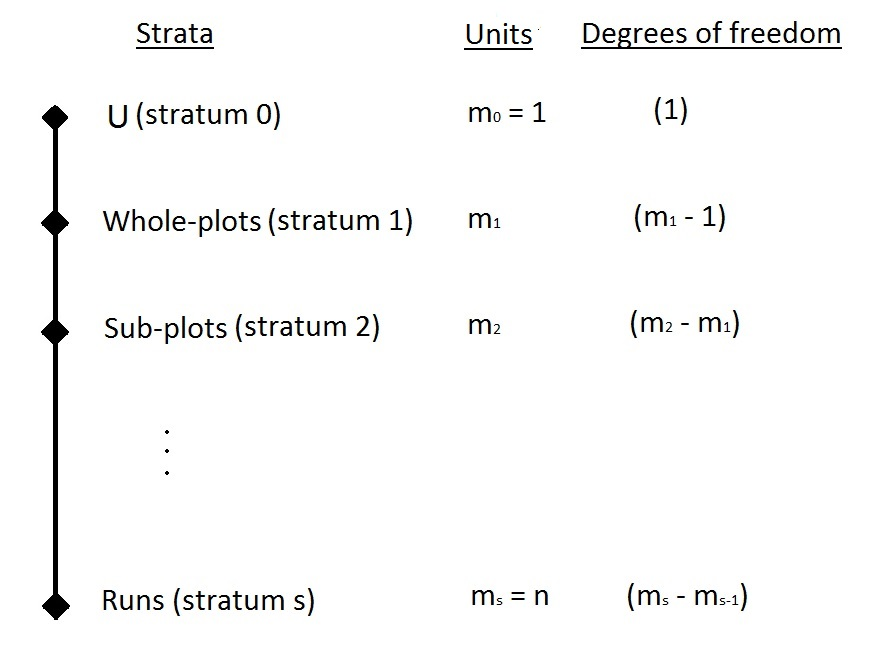
\includegraphics[scale=0.85]{Hasse.jpg}      %width=\textwidth
\caption{Hasse diagram for factors}
\label{Fig::Hasse}
\end{center}
\end{figure} 
 
Recall the expression for the linear polynomial hierarchical model from (\ref{eq::intro_ms}):
\begin{equation}
\label{eq::back_ms}
\bm{Y}=\bm{X}\bm{\beta}+\sum_{i=1}^{s}\bm{Z}_{i}\bm{\varepsilon}_{i},
\end{equation} 
where the first part $\bm{X\beta}$ contains the fixed effects, and $\sum_{i=1}^{s}\bm{Z}_{i}\bm{\varepsilon}_{i}$ stands for the random part, i.e.~it comprises information on variation occurring at each level of randomisation. All of the errors are assumed to be independent, having zero means and constant variances $\sigma^2_{i}$ and, as seen from the model formulation, additive.

In this case the fixed effects coefficients, $\bm{\beta}$ are usually estimated using the Generalised Least Square (GLS) formula:
\begin{equation}
\label{eq::back_gls}
\bm{\hat{\beta}}=(\bm{X}'\bm{VX})^{-1}\bm{X}'\bm{V}^{-1}Y,
\end{equation}
so that the variance of the estimators is
\begin{equation}
\label{eq::back_glsvar}
Var(\bm{\hat{\beta}})=(\bm{X}'\bm{VX})^{-1},
\end{equation}
where $\bm{V}$ is the variance-covariance matrix of the (normally distributed) responses, has a block-diagonal structure, and can be presented as:
\begin{equation}
\label{eq::back_glsV}
\bm{V}=\sum_{i=1}^{s}\sigma^2_{i}\bm{Z}_{i}\bm{Z}'_{i}=\sigma^{2}_{s}\left(\bm{I}_{n}+\sum_{i=1}^{s-1}\eta_{i}\bm{Z}_{i}\bm{Z}'_{i}\right).
\end{equation}
Here $\eta_{i}=\sigma^{2}_{i}/\sigma^{2}_{s}$ is defined as a variance ratio, denoting the magnitude of variability occurring at higher strata scaled with respect to the between-run variance.

At the analysis stage, as the variance components are unknown, their estimates are obtained and substituted in (\ref{eq::back_glsvar}) to obtain an estimated variance-covariance matrix of the parameters' estimators, $\bm{\hat{V}(\hat{\beta})}$; the estimation methods are discussed in more detail in Chapter \ref{ch::mse_ms}.

However, when an experiment is being planned, and none of the $\eta_{i}$ or $\sigma^2_{s}$ are known, there are two main approaches to deal with it. The first one is to search for designs assuming some point prior values of the $\eta$ parameter and, for these, evaluate the variance-based criteria, considering all strata simultaneously.

The case of split-plot experiments, with two strata, $\sigma^2_{s}=\sigma^2$ and $\eta=\sigma^2_{1}/\sigma^2$, has been extensively considered in the literature. \cite{Goos2001Doptimal} considered the three cases when D-optimal designs for split-plot experiments do not depend on the value of $\eta$; in other practical cases an estimate of the variance ratio is to be provided. \cite{Goos2003Doptimal} and \cite{Jones2007candidate} developed algorithms for finding $D$-optimal split-plot designs and for some examples demonstrated the robustness to the different values of $\eta$. An algorithm for constructing $D$-optimal split-split-plot designs can be found in the paper by \cite{Jones2009Doptimal}. 
%\cite{Goos2007tailor} -- split-plot for mixture experiments  

The Bayesian alternative to the `exhaustive search' approach across the unknown parameter space allows specifying a prior distribution on the unknown parameters, and then evaluating the criteria by integrating over that prior. \cite{Arnouts2012staggered} presented a coordinate-exchange algorithm for constructing D-optimal designs for a staggered experimental structure (i.e. values of hard-to-change factors' are changed at different time points), with log-normal prior distributions being put on the variance ratios. Later \cite{Arnouts2015staggered} studied the staggered structured designs in the context of response surface modelling, and considered a few examples of D- and I-optimal designs.
 
\cite{Mylona2014optimal} introduced a composite criterion, combining $D$-optimality for the fixed and variance components; in such an approach both the criterion formula and the form of the prior distributions define the way of evaluation the criterion function, which often leads to the necessity of choosing a computationally efficient numerical methodology. \cite{Gilmour2009analysis} proposed an appropriate Bayesian analysis strategy of data from multistratum experiments, that is robust to designs non-orthogonality and is shown to be more reliable than REML approach.  

However, in the general case a lot of computational effort might be required in order to be confident in the goodness of the design obtained by choosing from a set of assumed possible values of $\eta_i$, either using point priors or adapting general Bayesian strategy, especially when there are more than two strata and, therefore, the range of unknown parameters becomes multi-dimensional. The stratum-by-stratum approach (as first suggested by \cite{Trinca2001multistratum} and more recently improved by \cite{Trinca2015improved}) implies going from the highest stratum to the lowest, at each level choosing the set of treatments, and the units of higher level being treated as fixed block effects. Such methodology allows `protecting' against the case of large higher level variances, and eliminates the need for any prior information on unknown parameters. The authors later adapted the stratum-by-stratum  strategy for the inference criteria \citep{Trinca2016SPinference}, providing tools for constructing efficient designs for relatively small experiments in the presence of restricted randomisation.

\section{Accounting for Model Misspecification}
\label{sec::back_misspecification}
Standard optimality criteria usually rely on the assumption that the fitted model provides a (significantly) good fit for the data. However, as in many experiments this might be a concern, the possibility of model misspecification should be accounted for at the stage of planning. 

Lots of research has been conducted in this direction. In the cases when the form of model contamination is unknown, some authors adapt the approach of incorporating some prior knowledge regarding the possible functions representing the model departure from the data, for example, \cite{Notz1989Optimal} presented the methodology of optimal planning (with respect to the fitted model coefficients' estimates) while accounting for a presence of a bias function (that has $0$ expectation over the prior and finite second moment). In a similar view \cite{Wiens1993Designs} studied the construction of designs that minimise the effect of the unknown disturbance on the coverage probability of the confidence ellipsoid of the fitted model's parameters. \cite{Allen2003Experimental} proposed the expected integrated mean-squared error optimality criterion for maximising the prediction precision in the presence of potential model misspecification; \cite{Woods2005designing} accounted for (involving) a random additive model contamination in their optimality criteria for polynomial spline regression models.

When the form of the model deviation is assumed to be known, one of the most particular cases is when the fitted model is nested within the full one, and both of them are estimable; essentially the initial problem is reduced to model discrimination. One of the basic approaches for choosing between two polynomial models is $T$ -- optimality, the criterion first introduced by \cite{Atkinson1975Design} for discriminating between any two polynomials; a lot of research has been conducted based on this, e.g. \cite{Dette2012T} focused on constructing $T$-optimal designs when polynomials differ in degree by two. \cite{Dette1995Optimal} introduced a more general strategy of constructing designs optimal with respect to identifying the best suitable degree of the polynomial model to be fitted.

A series of works has been devoted to constructing designs such that their desirable properties would be robust to possible faults in model choice. For example, \cite{Wiens1992Minimax} introduced the minimax approach to the class of loss function that the author defined as monotonic functions of the mean squared error matrix ocurring from the model misspecification function coming from a bounded in $\mathcal{L}_2$ set. Later \cite{Wiens2009Robust} developed a general methodology of finding optimal sequential designs allowing for model discrimination and then, after the best model has been chosen, for efficient parameter estimation and/or prediction. \cite{Wiens2000Bias} aimed at minimising the maximum integrated mean squared error of the fitted values, where the maximum is found over the functional family of model deviations. 

The $\mathcal{Q}_{B}$ criterion, first introduced by \cite{Tsai2007Three}, aimed at taking advantage of experimenter's prior knowledge and providing efficient estimations of all models nested within the ``maximal model of interest'', was later generalised by \cite{Tsai2010General} and shown to be interpretable and statistically meaningful. \cite{Smucker2012Model} were the first ones to consider split-plot structures in this context; they introduced a `weighted' adaptation of $D$-optimality in order to obtain designs accounting not for one, but for a set of models.

In this thesis, due to the primary interest being the quality of inference, the view of model uncertainty will be strongly based on the approach developed by \cite{Goos2005model}, combining model-robust and model-sensitive approaches to design construction; it is examined in more detail in Chapter \ref{ch::generalised}. 

\section{Search Implementation: Point-Exchange Algorithm}

As mentioned above, in practice we work with exact designs, and there are quite a few options of how this search should be implemented.  

The design search methodology for a factorial experiment used here was first introduced in \citet{fedorov1972theory}. The candidate set of points is composed as the set of all possible combinations of the factors' levels. The algorithm starts with generating a random design from this set and, starting with the very first point in it, it goes through the candidate set, exchanges the current point in the current design with the `new' point from the candidate set and if the exchange improves the value of the criterion function, keeps the exchange. A number of random starts is usually set up, and the best design is kept in the end.

The coordinate-exchange algorithm, as a possible alternative, was first introduced by \cite{Meyer1995Coordinate} and since then has been widely used by various authors when searching for exact designs. It starts with generating a random initial design, and, as going through rows and columns of design matrix, the values of each element of the design matrix are being swapped among all the candidate values for the corresponding factor, and the criterion is evaluated; this is done till no improvement is achieved, and again, the whole procedure is repeated for some number of random starts. 

The obvious advantage is that there is no candidate set of design points required. It is more popular in experiments with hierarchical unit structures: \cite{Jones2007candidate} adapted the approach for constructing split-plot D-optimal designs, whilst \cite{Sambo2014Coordinate} proposed the coordinate-exchange two-phase local search (CE-TPLS), allowing simultaneous optimisation with respect to $D$- and $I$-optimality. Later \cite{Borrotti2016Multi} introduced the coordinate-exchange algorithm, now for multistratum design search and for several objectives (up to six optimality criteria), such that the whole Pareto front can be considered and the best design chosen.  

When working with multistratum designs, we essentially adopt the stratum-by-stratum approach presented by \cite{Trinca2016SPinference}, as further described in Chapter \ref{ch::mse_ms}. 

%%%%%%  






\chapter{Compound Criteria. Some Amendments}
\label{ch::compound}
In the discussion of the paper by \citet{GilmourTrinca2012}, among many comments and suggestions, two of them are of our particular interest if we research the ways of constructing optimality criteria reflecting various desirable inference properties:
\begin{itemize}
\item Designs which were obtained by optimising according to the $DP$- and/or $LP$-criterion tend to have most of the residual degrees of freedom allocated to the pure error component in the error variance decomposition thus creating an imbalance and even making the test for lack of fit impossible in the extreme case, when all available degrees of freedom are assigned to pure error. In Section \ref{sec::extraF} we consider an amendment of the criteria that could potentially result in some improvements.
\item In the construction of a compound criterion each component is essentially the identity function of an elementary efficiency; in other words, the impact of each individual component is proportional to the corresponding efficiency value. However, in some situations it might be sensible to alter the nature of this impact, for example, `cut off' the designs that perform below a certain threshold with respect to a particular component or, on the contrary, assume that all designs with efficiencies large enough are equally `good'. In Section \ref{sec::desfun} we will employ some desirability functions as the compound criterion components and will examine how this would affect the results. 
\end{itemize} 

\section{Extra F-quantile}
\label{sec::extraF}
If we are in the framework of an unblocked experiment and the fitted model is polynomial regression with $p$ parameters (\ref{eq::back_model}):
\begin{equation*}
\bm{Y}=\bm{\beta}_{0}+\bm{X\beta}+\bm{\varepsilon},
\end{equation*}
i.e. $p-1$ parameters of interest and the intercept being the nuisance parameter, we can decompose the full information matrix:
\begin{equation*}
%\label{eq::infmatrix}
\bm{M}=\left[ \begin{array}{c}\bm{1'}\\\bm{X'}\end{array} \right]\left[\begin{array}{cc}\bm{1} & \bm{X}\end{array}\right]=\left[\begin{array}{cc}
\bm{n} & \bm{1'X}\\ \bm{X'1} & \bm{X'X} 
\end{array}  \right].
\end{equation*}
Then the information matrix corresponding to all parameters except for the intercept, will look as follows:
\begin{equation}
\label{eq::s_infmatrix}
(\bm{M}^{-1}_{22})^{-1}=\bm{X'}\bm{Q}_{0}\bm{X}, \mbox{ where }\bm{Q}_{0}=\bm{I_n}-\frac{1}{n}\bm{11'}.  
\end{equation}
This representation is essentially a special case of the blocked experiment framework, described in Section \ref{sec::back_blocked}, with matrix of block indicators $\bm{Z}$ being an $(n\times 1)$ intercept column. 

Therefore the corresponding `pure error' optimality criteria  become (see also (\ref{eq::DPs_blocked}) and (\ref{eq::LPs_blocked})): 
\begin{align}
\label{eq::DPs_inter}
DP_S: \mbox{minimise } &(F_{p-1,d;1-\alpha_{DP}})^{p-1}\vert (\bm{X'}\bm{Q}_{0}\bm{X})^{-1}\vert,\\
\label{eq::LPs_inter}
LP_S: \mbox{minimise } &F_{1,d;1-\alpha_{LP}}\mbox{tr}\{\bm{W}(\bm{X'}\bm{Q}_{0}\bm{X})^{-1}\}.
\end{align}

Martina Vandebroek in the discussion of the paper by \cite{GilmourTrinca2012} (p.~$373$) suggested including an extra $F$-quantile as a compound criterion component which would guarantee some degrees of freedom for both pure error and lack-of-fit parts. 

To test the model for the lack of fit, the following test statistic might be used:
\begin{equation*}
\frac{LoF\mbox{ }SS/(n-p-d)}{Pure\mbox{ }Error\mbox{ }SS/d} \sim F_{n-p-d,d}.
\end{equation*}
In a similar way as before, the `lack-of-fit', $LoF$-efficiency can be defined:
\begin{equation}
\label{eq::LoF_eff}
\mbox{Eff}_{LoF}(\bm{X})=\frac{F_{n-p-d_{*},d_{*};1-\alpha_{LoF}}}{F_{n-p-d,d;1-\alpha_{LoF}}},
\end{equation}
where $d_{*}$ is the number of pure error degrees of freedom of the optimal design $\bm{X}_{*}$ in terms of maximising $1/F_{n-p-d,d;1-\alpha_{LoF}}$ or, equivalently, minimising $F_{n-p-d,d;1-\alpha_{LoF}}$. The scale of such representation is in accordance with the previously defined $D$-efficiency in (\ref{eq::D_eff}), and with the accordingly defined $DP_S$-efficiency:
\begin{equation}
\mbox{Eff}_{DP_S}(\bm{X})=\frac{F_{p-1,d_{*};1-\alpha_{DP}}\vert(\bm{X_{*}}'\bm{Q}_{0}\bm{X_{*}})^{-1}\vert ^{1/p-1}}{F_{p-1,d;1-\alpha_{DP}}\vert(\bm{X}'\bm{Q}_{0}\bm{X})^{-1}\vert ^{1/p-1}}.
\end{equation}

In Figure \ref{Fig::extraF} the values of the inverse $F$-quantile are presented depending on the pure error degrees of freedom for three different scenarios of available residual degrees of freedom: $19$, $25$ and $30$. In all cases the curvatures are clearly convex, so that maximum values exist and they are unique in every given case. Larger numbers of available residual degrees of freedom correspond to the larger `optimal' pure error degrees of freedom, i.e. where the maximum of the inverse F-quantile is achieved. For example, when $n-p$ is equal to $19$, the optimal $d$ is $12$, and for $n-p=30$ the maximum of $F_{n-p-d,d;1-\alpha_{LoF}}$ is at $d=19$.

% F-percentile
\begin{figure}[ht]
\begin{center}
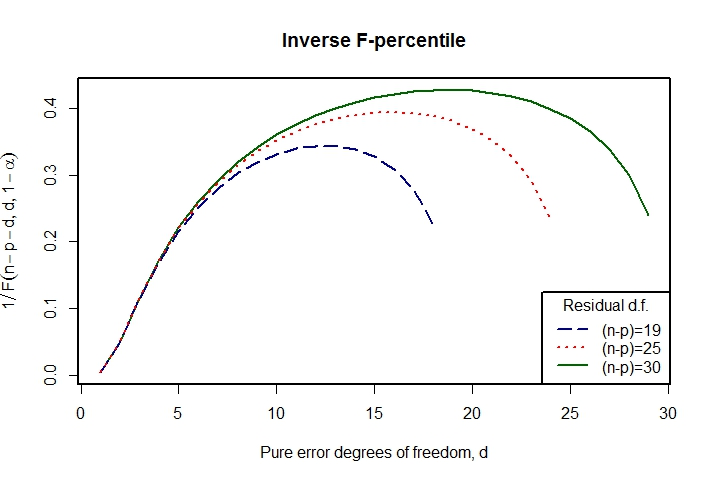
\includegraphics[scale=0.7]{Fquantile.jpeg}
\caption{Inverse F-quantile vs Pure Error degrees of freedom, $d$}
\label{Fig::extraF}
\end{center}
\end{figure}

Adding this element (\ref{eq::LoF_eff}) to the components responsible for the point and interval precision of the parameters' estimates: $D_S$ and $DP_S$ (or $L_S$ and $LP_S$) and the $DF$ criterion defined in (\ref{eq::DF_eff}), we get the following determinant and trace-based functions to be minimised:
\begin{align}
\label{eq::ExtraFD_crit}
\vert\bm{X}'\bm{Q_{0}}\bm{X}\vert^{-\frac{\kappa_D}{(p-1)}}\times \left[F_{p-1,d;1-\alpha_{DP}}\vert\bm{X'}\bm{Q_{0}}\bm{X}\vert^{-\frac{1}{(p-1)}}\right]^{\kappa_{DP}}\times(n-d)^{\kappa_{DF}}\times \notag \\ \left[F_{n-p-d,d;1-\alpha_{LoF}}\right]^{\kappa_{LoF}}
\end{align}
and
\begin{align}
\label{eq::ExtraFL_crit}
\left[\mbox{trace}\{\bm{W}(\bm{X'}\bm{Q_{0}}\bm{X})^{-1}\}\right]^{\kappa_L+\kappa_{LP}}\times\left[F_{1,d;1-\alpha_{LP}}\right]^{\kappa_{LP}}\times (n-d)^{\kappa_{DF}}\times\left[F_{n-p-d,d;1-\alpha_{LoF}}\right],^{\kappa_{LoF}}
\end{align}
where, as before, $d$ stands for the number of pure error degrees of freedom or, equivalently, the number of replicated points in the model matrix $\bm{X}$. The significance levels $\alpha_{DP}$ and $\alpha_{LoF}$ are usually set to $0.05$; correction for multiple comparisons is applied to the $LP_s$-component, as given in (\ref{eq::Sidak}), and $\alpha_{LP}$ is amended accordingly. The third component in both criteria corresponds to the DF-efficiency defined in (\ref{eq::DF_eff}).
 
\subsection{Optimal designs accounting for the model lack-of-fit}
\label{sec::optimal_extraF}
The following example was considered in order to compare optimal designs obtained for various compound criteria consisting of weighted combinations of $D_S$-, $DP_S$-, $DF$- and $LoF$-efficiencies. 
Designs were derived for a factorial experiment with five explanatory factors, each of three levels, and with only $40$ runs. The full second-order polynomial model is to be fitted, i.e. the number of parameters $p=21.$ The intercept is a nuisance parameter, and so further on we will be dealing with optimality criteria only for the parameters of interest. However, in the notation the subscript $S$ shall be omitted.

The resulting design is to be chosen (in other words, sampled with replacement) from the candidate set of points containing $3^{5}=243$ possible combinations of factors' values. A standard point exchange algorithm with $500$ random starts was used to find the optimal combination (as described before and the same as was used in \citealp{GilmourTrinca2012}).

In Table \ref{Table_extraFD} each row corresponds to the optimal design obtained with respect to the criterion function (\ref{eq::ExtraFD_crit}) with the weights given in the first columns; then the degrees of freedom (DoF) for pure error (PE) and lack of fit (LoF) are presented together with the individual efficiencies of the designs. Zero values there indicate the cases when a certain component ($DP$, $LP$ or $LoF$) cannot be estimated due to the absence of replicates in the design. 

Some expected features might be noticed here: designs which perform well in terms of the $D$-criterion generally have quite large $L$-efficiency values (and a similar tendency holds for $DP$- and $LP$-efficiencies). When all the components are equally weighted (design \#$12$), the resulting design performs well in terms of all the criteria, all efficiencies are above $90\%$.  

\begin{table}[h]
\centering
\caption{Example 1. Properties of optimal designs with respect to determinant-based compound criteria with an extra F-quantile}
\label{Table_extraFD}
\scalebox{0.8}{
%\resizebox{\textwidth}{!}} \\
\multicolumn{1}{l}{} & \textbf{D} & \textbf{DP} & \textbf{DF} & \textbf{LoF} & \textbf{PE} & \textbf{LoF} & \textbf{D} & \textbf{DP} & \textbf{L} & \textbf{LP} & \textbf{LoF} & \textbf{DF}\\
1 & 1 & 0 & 0 & 0 & 0 & 19 & 100.00 & 0.00 & 99.67 & 0.00 & 0.00 & 100.00 \\
2 & 0 & 1 & 0 & 0 & 18 & 1 & 93.00 & 100.00 & 79.32 & 93.01 & 66.00 & 55.00\\
3 & 0.5 & 0.5 & 0 & 0 & 16 & 3 & 95.29 & 98.64 & 79.96 & 92.09 & 89.95 & 60.00 \\
4 & 0.5 & 0 & 0.5 & 0 & 0 & 19 & 100.00 & 0.00 & 99.67 & 0.00 & 0.00 & 100.00\\
5 & 0.5 & 0 & 0 & 0.5 & 12 & 7 & 97.59 & 90.38 & 90.24 & 98.39 & 100.00 & 70.00\\
6 & 0 & 0.5 & 0.5 & 0 & 12 & 7 & 97.62 & 90.40 & 90.63 & 98.81 & 100.00& 70.00\\
7 & 0 & 0.5 & 0 & 0.5 & 14 & 5 & 96.93 & 95.61 & 88.12 & 98.19 & 98.48 & 65.00\\
8 & 0 & 0 & 0.5 & 0.5 & 10 & 9 & 49.77 & 42.27 & 25.19 & 26.26 & 96.46 & 75.00\\
9 & 1/3 & 1/3 & 1/3 & 0 & 12 & 7 & 97.60 & 90.38 & 90.19 & 98.33 & 100.00& 70.00\\
10 & 1/3 & 1/3 & 0 & 1/3 & 14 & 5 & 96.93 & 95.61 & 87.27 & 98.19 & 98.48 & 65.00\\
11 & 0 & 1/3 & 1/3 & 1/3 & 12 & 7 & 97.60 & 90.38 & 90.19 & 98.33 & 100.00 & 70.00\\
12 & 0.25 & 0.25 & 0.25 & 0.25 & 12 & 7 & 97.62 & 90.40 & 90.63 & 98.81 & 100.00 & 70.00\\
\end{tabular}
}
\end{table} 
It is also noticeable that the $D$-optimal design (\#$1$) retains its optimality when half of the weight is allocated to the $DF$-component, i.e. with $\kappa_{D}=\kappa_{DF}=0.5$ (\#$4$), and it contains no replicates. The design itself is presented in Table \ref{tab::design1} (with the points ordered for the sake of perception): it can be seen that the design points are more or less evenly distributed over the design space, with one centre point and with half of the points being `corner' ones, i.e. when all factors take the values $\pm1$. 

All other designs have more degrees of freedom allocated to the pure error component than to the lack-of-fit one and, therefore, their $DF$-efficiency values $\frac{n-d}{n}$ are below $75\%$ (i.e. when $d>10$). The maximum of the lack-of-fit efficiency is achieved when $d=12$, and the balance in the allocation of degrees of freedom was obtained when the total weight was equally distributed between the $DF$- and $LoF$-components, so that design \#$8$ given in the table is quite arbitrary and can be replaced with any other having $10$ pure error degrees of freedom. Further improvements of the performance in terms of other components can be achieved, for example, by setting a constraint on the degrees of freedom.
\begin{table}[h]
\centering
\caption{Example 1. D-optimal design (\#$1$ and \#$4$)}
\label{tab::design1}
\scalebox{0.8}{
\begin{tabular}{rrrrrr|r|rrrrrr}
1  & -1 & -1 & -1 & -1 & 1  &  & 21 & 0 & 1  & -1 & -1 & -1 \\
2  & -1 & -1 & -1 & 1  & -1 &  & 22 & 0 & 1  & 0  & -1 & 1  \\
3  & -1 & -1 & -1 & 1  & 1  &  & 23 & 0 & 1  & 1  & 1  & -1 \\
4  & -1 & -1 & 0  & -1 & -1 &  & 24 & 1 & -1 & -1 & -1 & -1 \\
5  & -1 & -1 & 1  & -1 & 1  &  & 25 & 1 & -1 & -1 & -1 & 1  \\
6  & -1 & -1 & 1  & 1  & -1 &  & 26 & 1 & -1 & -1 & 1  & 0  \\
7  & -1 & -1 & 1  & 1  & 1  &  & 27 & 1 & -1 & 0  & 0  & 1  \\
8  & -1 & 0  & -1 & -1 & -1 &  & 28 & 1 & -1 & 1  & -1 & -1 \\
9  & -1 & 0  & 1  & 0  & -1 &  & 29 & 1 & -1 & 1  & 1  & -1 \\
10 & -1 & 1  & -1 & -1 & 0  &  & 30 & 1 & -1 & 1  & 1  & 1  \\
11 & -1 & 1  & -1 & 0  & 1  &  & 31 & 1 & 0  & -1 & -1 & 0  \\
12 & -1 & 1  & -1 & 1  & -1 &  & 32 & 1 & 0  & 0  & 1  & -1 \\
13 & -1 & 1  & 0  & 1  & 0  &  & 33 & 1 & 0  & 1  & -1 & 1  \\
14 & -1 & 1  & 1  & -1 & -1 &  & 34 & 1 & 1  & -1 & -1 & 1  \\
15 & -1 & 1  & 1  & -1 & 1  &  & 35 & 1 & 1  & -1 & 0  & -1 \\
16 & -1 & 1  & 1  & 1  & 1  &  & 36 & 1 & 1  & -1 & 1  & -1 \\
17 & 0  & -1 & -1 & 0  & -1 &  & 37 & 1 & 1  & -1 & 1  & 1  \\
18 & 0  & -1 & 1  & -1 & 0  &  & 38 & 1 & 1  & 1  & -1 & -1 \\
19 & 0  & 0  & -1 & 1  & 1  &  & 39 & 1 & 1  & 1  & 0  & 0  \\
20 & 0  & 0  & 0  & 0  & 0  &  & 40 & 1 & 1  & 1  & 1  & 1 
\end{tabular}
}
\end{table} 
Whether equal weights are distributed between $DP$ and $LoF$ components of the compound criterion or between $D$, $DP$ and $LoF$, the resulting designs are the same (\#$7$ and \#$10$), providing quite large $DP$-, $LP$- and $LoF$-efficiency values and fairly high $D$-efficiency. The design can be found in Table \ref{tab::design7}: all of its pure error degrees of freedom occur from the single replicates of the corner points, there is no centre point and in general fewer points contain any factors at the zero level in comparison to the $D$-optimal design observed before.

\begin{table}[h]
\centering
\caption{Example 1. Optimal design with respect to the determinant based-criteria \#$7$ and \#$10$}
\label{tab::design7}
\scalebox{0.8}{
\begin{tabular}{rrrrrr|r|rrrrrr}
1  & -1 & -1 & -1 & -1 & 1  &  & 21 & 0 & 0  & -1 & -1 & 0  \\
2  & -1 & -1 & -1 & -1 & 1  &  & 22 & 0 & 0  & 0  & 1  & 1  \\
3  & -1 & -1 & -1 & 1  & -1 &  & 23 & 0 & 1  & 1  & 0  & 1  \\
4  & -1 & -1 & -1 & 1  & -1 &  & 24 & 1 & -1 & -1 & -1 & -1 \\
5  & -1 & -1 & 1  & -1 & -1 &  & 25 & 1 & -1 & -1 & -1 & -1 \\
6  & -1 & -1 & 1  & 1  & 1  &  & 26 & 1 & -1 & -1 & 1  & 1  \\
7  & -1 & -1 & 1  & 1  & 1  &  & 27 & 1 & -1 & -1 & 1  & 1  \\
8  & -1 & 0  & -1 & 0  & 0  &  & 28 & 1 & -1 & 1  & -1 & 1  \\
9  & -1 & 0  & 0  & 0  & -1 &  & 29 & 1 & -1 & 1  & -1 & 1  \\
10 & -1 & 0  & 1  & -1 & 1  &  & 30 & 1 & -1 & 1  & 1  & -1 \\
11 & -1 & 1  & -1 & -1 & -1 &  & 31 & 1 & -1 & 1  & 1  & -1 \\
12 & -1 & 1  & -1 & -1 & -1 &  & 32 & 1 & 1  & -1 & -1 & 1  \\
13 & -1 & 1  & -1 & 1  & 1  &  & 33 & 1 & 1  & -1 & -1 & 1  \\
14 & -1 & 1  & -1 & 1  & 1  &  & 34 & 1 & 1  & -1 & 1  & -1 \\
15 & -1 & 1  & 0  & -1 & 1  &  & 35 & 1 & 1  & -1 & 1  & -1 \\
16 & -1 & 1  & 1  & -1 & 0  &  & 36 & 1 & 1  & 0  & 0  & 0  \\
17 & -1 & 1  & 1  & 1  & -1 &  & 37 & 1 & 1  & 1  & -1 & -1 \\
18 & -1 & 1  & 1  & 1  & -1 &  & 38 & 1 & 1  & 1  & -1 & -1 \\
19 & 0  & -1 & 0  & -1 & 0  &  & 39 & 1 & 1  & 1  & 1  & 1  \\
20 & 0  & -1 & 1  & 0  & -1 &  & 40 & 1 & 1  & 1  & 1  & 1 
\end{tabular}
}
\end{table}
Also the same design is optimal according to the criteria \#$9$ and \#$11$ (and it is quite similar to the optimal design with respect to the equal-weighted criterion \#$12$), such that a little weight reallocation in this case does not substantially affect the performance.

Optimal designs with respect to similar trace-based criteria are presented in Table \ref{Table_extraFL}. On the whole, the relationships between the weights of the criteria and resulting designs' efficiencies are similar to the ones seen above. However, here one can observe more variability in the distribution of the degrees of freedom between the pure error and lack-of-fit components: designs \#$6$ and \#$9$ have $8$ pure error degrees of freedom, although, their $DP$-efficiencies are lower than  usual (approximately $72\%$ instead of up to $90\%$). In addition, the design optimal according to the equal-weighted criterion (\#$12$) is also optimal with respect to the criterion with equal weights put on the $DF$- and $LoF$-components as it has the balanced allocation of degrees of freedom; it is presented in Table \ref{tab::Ldesign9} below as an illustration of a compromise between the different components of the trace-based criterion.     

\begin{table}[h]
\centering
\caption{Example 1. Properties of optimal designs with respect to trace-based compound criteria with an extra F-quantile}
\label{Table_extraFL}
\scalebox{0.8}{
%\resizebox{\textwidth}{!}} \\
\textbf{} & \textbf{L} & \textbf{LP} & \textbf{DF} & \textbf{LoF} & \textbf{PE} & \textbf{LoF} & \textbf{D} & \textbf{DP} & \textbf{L} & \textbf{LP} & \textbf{LoF} & \textbf{DF} \\
1 & 1 & 0 & 0 & 0 & 0 & 19 & 99.95 & 0.00 & 100.00 & 0.00 & 0.00 & 100.00\\
2 & 0 & 1 & 0 & 0 & 14 & 5 & 95.01 & 93.72 & 88.88 & 100.00 & 98.48 & 65.00 \\
3 & 0.5 & 0.5 & 0 & 0 & 11 & 8 & 97.18 & 86.50 & 92.83 & 99.18 & 98.83 & 72.50 \\
4 & 0.5 & 0 & 0.5 & 0 & 0 & 19 & 99.95 & 0.00 & 100.00 & 0.00 & 0.00 & 100.00\\
5 & 0.5 & 0 & 0 & 0.5 & 12 & 7 & 96.69 & 89.54 & 91.71 & 99.99 & 100.00 & 70.00\\
6 & 0 & 0.5 & 0.5 & 0 & 8 & 11 & 97.10 & 72.60 & 95.61 & 93.06 & 87.94 & 80.00 \\
7 & 0 & 0.5 & 0 & 0.5 & 13 & 6 & 95.55 & 91.54 & 90.11 & 99.93 & 99.93 & 67.50 \\
8 & 0 & 0 & 0.5 & 0.5 & 10 & 9 & 49.77 & 42.27 & 25.19 & 26.26 & 96.46 & 75.00\\
9 & 1/3 & 1/3 & 1/3 & 0 & 8 & 11 & 96.75 & 72.34 & 95.35 & 92.80 & 87.94 & 80.00\\
10 & 1/3 & 1/3 & 0 & 1/3 & 12 & 7 & 96.69 & 89.54 & 91.71 & 99.99 & 100.00 & 70.00\\
11 & 0 & 1/3 & 1/3 & 1/3 & 11 & 8 & 96.65 & 86.02 & 92.74 & 99.09 & 98.83 & 72.50\\
12 & 0.25 & 0.25 & 0.25 & 0.25 & 10 & 9 & 96.91 & 82.29 & 93.99 & 97.98 & 96.46 & 75.00
\end{tabular}
}
\end{table} 

\begin{table}[h]
\centering
\caption{Example 1. Optimal design with respect to the trace based-criterion \#$12$}
\label{tab::Ldesign9}
\scalebox{0.8}{
\begin{tabular}{rrrrrr|r|rrrrrr}
1  & -1 & -1 & -1 & -1 & -1 &  & 21 & 0 & 0  & 1  & 1  & 0  \\
2  & -1 & -1 & -1 & -1 & 0  &  & 22 & 0 & 1  & -1 & -1 & -1 \\
3  & -1 & -1 & -1 & 1  & 1  &  & 23 & 0 & 1  & -1 & 1  & 0  \\
4  & -1 & -1 & -1 & 1  & 1  &  & 24 & 0 & 1  & 1  & -1 & 1  \\
5  & -1 & -1 & 1  & -1 & 1  &  & 25 & 1 & -1 & -1 & -1 & 1  \\
6  & -1 & -1 & 1  & 1  & -1 &  & 26 & 1 & -1 & -1 & -1 & 1  \\
7  & -1 & -1 & 1  & 1  & -1 &  & 27 & 1 & -1 & -1 & 1  & -1 \\
8  & -1 & 0  & -1 & 1  & -1 &  & 28 & 1 & -1 & -1 & 1  & -1 \\
9  & -1 & 0  & 0  & -1 & 1  &  & 29 & 1 & -1 & 1  & -1 & -1 \\
10 & -1 & 0  & 1  & 0  & 0  &  & 30 & 1 & -1 & 1  & -1 & -1 \\
11 & -1 & 1  & -1 & -1 & 1  &  & 31 & 1 & -1 & 1  & 1  & 1  \\
12 & -1 & 1  & -1 & 0  & 0  &  & 32 & 1 & 0  & -1 & -1 & -1 \\
13 & -1 & 1  & 0  & 1  & -1 &  & 33 & 1 & 0  & 0  & 1  & 1  \\
14 & -1 & 1  & 1  & -1 & -1 &  & 34 & 1 & 1  & -1 & 0  & -1 \\
15 & -1 & 1  & 1  & -1 & -1 &  & 35 & 1 & 1  & -1 & 1  & 1  \\
16 & -1 & 1  & 1  & 1  & 1  &  & 36 & 1 & 1  & 0  & -1 & 0  \\
17 & -1 & 1  & 1  & 1  & 1  &  & 37 & 1 & 1  & 0  & -1 & 0  \\
18 & 0  & -1 & 0  & 0  & -1 &  & 38 & 1 & 1  & 1  & 0  & 1  \\
19 & 0  & -1 & 0  & 0  & -1 &  & 39 & 1 & 1  & 1  & 1  & -1 \\
20 & 0  & 0  & -1 & 0  & 1  &  & 40 & 1 & 1  & 1  & 1  & -1
\end{tabular}
}
\end{table}

Again all the replicated points are the `corner' ones, except for the point number $18-19$ and the point number $36-37$; points are scattered across the design region, but at fewer than half of the runs at least one factor is applied at its $0$ level.

We also considered a slightly larger example of an experimental framework: four five-level factors (i.e. $625$ candidate points), $60$ runs and the full quadratic polynomial ($p=15$) as the fitted model. The corresponding efficiency tables can be found in Appendix \ref{appendix::ExtraF}. All optimal designs for both examples are provided in the Supplementary material, together with the corresponding R code files.

The search algorithm takes approximately three times longer than in the first example. Regarding the resulting designs, they also perform quite well in general, and, despite a larger number of residual degrees of freedom available ($45$), the majority of optimal designs tend to have either $15$, or $20$ or $30$ of them allocated to pure error, with a bit more variability in the case of the trace-based criteria. 

In both observed examples it might seem that $D$ and $DF$ parts of the compound criteria tend to introduce similar properties into the optimal designs (and $DP$ together with $LoF$ components); the same is true for $L$ and $LP$ components. It is worth noticing that if some weight is allocated to at least three components, the designs perform quite well with respect to all elementary criteria. However, even if no unpredictable or completely uninterpretable effects are observed, there is no obvious pattern which would allow discovering a clear relation between weight allocation in the compound criterion and the resulting efficiency values. It also would be sensible to explore the ways to incorporate testing for model lack-of-fit in the optimality criteria. 
 
\section{Desirability Function}
\label{sec::desfun}
\citet{Myers2009} described the concept of desirability functions in the context of optimisation of multiple responses; this approach can be adapted to defining compound criteria, i.e. including desirability functions of efficiencies  instead of efficiencies themselves. In this case a transformation that rearranges the importance of small/large efficiency values might be useful. For example, 
\begin{equation}
\label{eq::des_fun_trivial}
d(\mbox{Eff}(\bm{X}))=\begin{cases}0 & 0<\mbox{Eff}(\bm{X})\leq A, \\
\frac{\mbox{Eff}(\bm{X})-A}{B-A} & A<\mbox{Eff}(\bm{X})<B, \\
1 & B\leq \mbox{Eff}(\bm{X}),
\end{cases}
\end{equation}
for some chosen lower and upper bounds $A$ and $B$.

The search for optimal designs using desirability functions was first performed for the elementary parameterisation given in (\ref{eq::des_fun_trivial}). Lower and upper bounds $A$ and $B$ were set to be equal to $0.2$ and $0.95$ respectively, the same for all components of the criteria: efficiency values that are lower than $20\%$ are all considered as being equally too small to be taken into account when assessing the design performance. On the other hand, all efficiency values that are larger than $95\%$ are treated as being equally satisfactory. A small change of the efficiency value within the interval $[A,B]$ results in a larger change of the correspondent component's impact on the resulting criterion value. 
 
The results of implementing the search procedure in this case demonstrate a certain inflexibility and  roughness of the linear piecewise desirability function: the point exchange algorithm stops the search once an appropriately large efficiency value is obtained (which is, obviously, not always the best possible value) due to the constant values of the function on the upper interval. The `jump' of the function for the argument values lying around the middle point $0.5$ is not, however, sharp enough to  support the suggestion that this approach is worth to be used instead of the initial one, especially taking into consideration that it is more time consuming. The main advantage, although, is that it does not allow for efficiencies below the determined threshold.

\subsection{Example of a smoothing function}
Because of the inflexibility observed in the case of linear parameterisation, it was decided to try another family of functions, which would satisfy the initial requirements and at the same time would be more flexible and allow finding the best possible designs. In this thesis we suggest the following smoothing transformation which is used as a desirability function, after being scaled to the $[0,1]$ interval: 
\begin{equation}
\label{eq::des_fun_exp}
f(x)=
\begin{cases}      
\exp(x^l),\mbox{                     } 0\leq x \leq 1/2\\
2\exp((1/2)^l)-\exp((1-x)^l),\mbox{  } 1/2 < x\leq 1, 
\end{cases}
\end{equation}
where $l\in\{1,2,\ldots \}.$

The Figure \ref{Fig::des_fun} contains plots of the (scaled) desirability function $f(x)$ itself, for three values of the parameter ($l=2,6$ and $15$) along with plots of the corresponding derivative functions that allow evaluating the rapidity of the function's change for different parameter values.
% Desirability function and its derivative
\begin{figure}[h]
\begin{center}
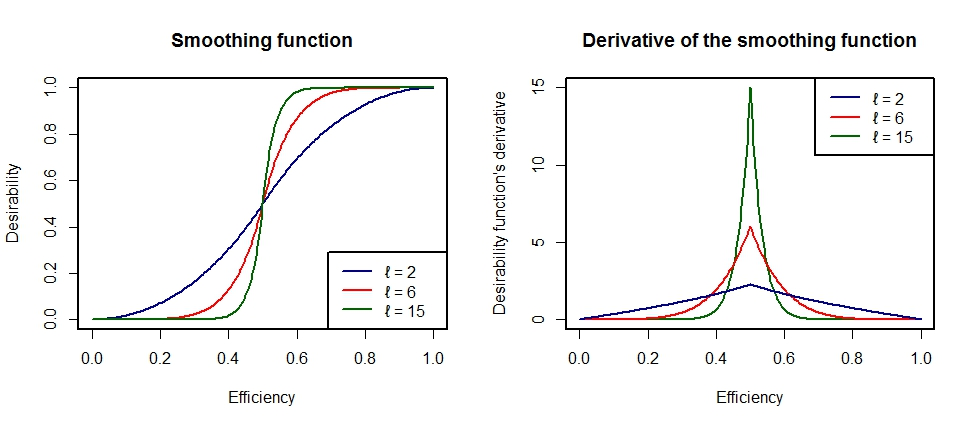
\includegraphics[width=\textwidth]{DesFunPlot.jpg}
\caption{Desirability function parameterisation and its derivative}
\label{Fig::des_fun}
\end{center}
\end{figure}
It can be seen that the function increases slowly at first and then, after a certain value depending on the parameter $l$ it makes a very sharp jump (larger values of $l$ correspond to faster jumps) and slowly reaches its maximum. This particular parameterisation makes the desirability function most sensitive to the changes of the efficiencies around $0.5$ which should result in considerable prevalence of the designs which are more than $50\%$ efficient. The value of $l$ was chosen to be equal to $6$ as a compromise between the slow and fast desirability increase rates in the middle region.

\subsection{Optimal designs}
The optimum design search was implemented for the first example described earlier: a three-factor experiment with each factor comprising three levels; with $40$ runs and $p=21$ parameters in the full quadratic polynomial model. As before, the interest is in all parameters except for the intercept; and the point exchange algorithm was used to find the designs maximising the following criterion function:
\begin{multline*}
\left[f(\mbox{Eff}_D(\bm{X}))\right]^{\kappa_D}\left[f(\mbox{Eff}_{DP}(\bm{X}))\right]^{\kappa_{DP}}\left[f(\mbox{Eff}_{DF}(\bm{X}))\right]^{\kappa_{DF}}\left[f(\mbox{Eff}_{LoF}(\bm{X}))\right],^{\kappa_{LoF}}
\end{multline*}
where the non-negative weights are to follow the same restriction as before: 
\begin{equation*}
\kappa_{D}+\kappa_{DP}+\kappa_{DF}+\kappa_{LoF}=1.
\end{equation*} 

Since here we utilise the function of the efficiencies at each step of the search, before using any composite criterion it is necessary to obtain optimality values of the elementary criteria involved: $D$, $DP$, $L$, $LP$, $DF$ and $LoF$ (the latter two are quite apparent, though), as we cannot just calculate the criteria functions directly when searching for the design. In this particular case we take the same $f(x)$ for every component, however, of course, different forms of the desirability function can be used as long as they are constructed appropriately and satisfy the restrictions (i.e. defined for all $x\in[0,1]$ and $f:[0,1]\rightarrow[0,1]$).    
 
The results for the determinant and trace-based criteria are summarised in Tables \ref{Table_DesFunD} and \ref{Table_DesFunL} respectively, where, as before, the efficiencies of the designs in terms of various primary criteria are given together with the allocation of residual degrees of freedom between the pure error and lack-of-fit components. It can be noticed that this parameterisation is rather sensitive and allows finding the best or almost the best designs; the $D$-efficiency for the `$D$-optimal' design \#$1$ is equal to $99.79\%$ ($99.61\%$ for the `$L$-optimal').

\begin{table}[h]
\centering
\caption{Example 1. Properties of optimal designs in terms of determinant-based compound criteria constructed with desirability functions}
\label{Table_DesFunD}
\scalebox{0.8}{
%\resizebox{\textwidth}{!}} \\
 & \textbf{D} & \textbf{DP} & \textbf{DF} & \textbf{LoF} & \textbf{PE} & \textbf{LoF} & \textbf{D} & \textbf{DP} & \textbf{L} & \textbf{LP} & \textbf{LoF} & \textbf{DF} \\
1 & 1 & 0 & 0 & 0 & 0 & 19 & 99.79 & 0.00 & 99.42 & 0.00 & 0.00 & 100.00\\
2 & 0 & 1 & 0 & 0 & 18 & 1 & 92.81 & 99.79 & 79.26 & 92.94 & 66.00 & 55.00\\
3 & 0.5 & 0.5 & 0 & 0 & 15 & 4 & 96.15 & 97.31 & 84.34 & 96.09 & 95.35 & 62.50\\
4 & 0.5 & 0 & 0.5 & 0 & 0 & 19 & 99.95 & 0.00 & 100.00 & 0.00 & 0.00 & 100.00\\
5 & 0.5 & 0 & 0 & 0.5 & 11 & 8 & 97.87 & 87.11 & 91.53 & 97.79 & 98.83 & 72.50\\
6 & 0 & 0.5 & 0.5 & 0 & 9 & 10 & 98.36 & 78.90 & 94.32 & 95.40 & 92.86 & 77.50\\
7 & 0 & 0.5 & 0 & 0.5 & 14 & 5 & 96.93 & 95.61 & 87.27 & 98.19 & 98.48 & 65.00\\
8 & 0 & 0 & 0.5 & 0.5 & 8 & 11 & 45.20 & 33.80 & 17.06 & 16.60 & 87.94 & 80.00\\
9 & 1/3 & 1/3 & 1/3 & 0 & 9 & 10 & 98.42 & 78.95 & 93.63 & 94.70 & 92.86 & 77.50\\
10 & 1/3 & 1/3 & 0 & 1/3 & 9 & 10 & 98.42 & 78.95 & 93.63 & 94.70 & 92.86 & 77.50\\
11 & 0 & 1/3 & 1/3 & 1/3 & 9 & 10 & 98.30 & 78.95 & 94.19 & 95.26 & 92.86 & 77.50\\
12 & 0.25 & 0.25 & 0.25 & 0.25 & 9 & 10 & 98.36 & 78.90 & 94.32 & 95.40 & 92.86 & 77.50\\
\end{tabular}
}
\end{table}

In general, comparing with the designs in the previous section, the distribution of the residual degrees of freedom was affected by using the desirability functions: now the numbers of pure error degrees of freedom is generally smaller, so often more of the available degrees of freedom are allocated to the lack-of-fit. Even the criterion \#$8$, whose value depends only on the degrees of freedom, in this case does not provide the best result: $8$ instead of the optimal $10$ pure error degrees of freedom. 

The current parameterisation provides quite large impact for the efficiency values around $50-80\%$, and one of the consequences is that the search may stop while in reality finding a considerably worse design. For example, design \#$10$ (the same as \#$9$) in Table \ref{Table_DesFunD} is $78.95\%$ $DP$-efficient, as the efficiency of the real optimal design according to this composite criterion, with $1/3$ allocated to the $DP$-component, is $95.61\%$ (as in Table \ref{Table_extraFD}). The fact is that the desirability function (\ref{eq::des_fun_exp}) $f(0.7895)=0.9972$, i.e. the transformed efficiency of $99.72\%$ is actually larger than the `true' one. In the meantime, the $D$-efficiency has increased by approximately $1.5\%$ (the corresponding weight is $1/3$ as well); and the current design contains fewer replicates, the number of pure error degrees of freedom is equal to $9$ in comparison to $14$ obtained previously (Table \ref{Table_extraFD}).

\begin{table}[h]
\centering
\caption{Example 1. Properties of optimal designs in terms of trace-based compound criteria constructed with desirability functions}
\label{Table_DesFunL}
\scalebox{0.8}{
%\resizebox{\textwidth}{!}} \\
 & \textbf{L} & \textbf{LP} & \textbf{DF} & \textbf{LoF} & \textbf{PE} & \textbf{LoF} & \textbf{D} & \textbf{DP} & \textbf{L} & \textbf{LP} & \textbf{LoF} & \textbf{DF} \\
1 & 1 & 0 & 0 & 0 & 0 & 19 & 99.03 & 0.00 & 99.61 & 0.00 & 0.00 & 100.00\\
2 & 0 & 1 & 0 & 0 & 13 & 6 & 96.49 & 92.44 & 90.04 & 99.85 & 99.93 & 67.50\\
3 & 0.5 & 0.5 & 0 & 0 & 9 & 10 & 96.91 & 77.74 & 94.53 & 95.61 & 92.86 & 77.50\\
4 & 0.5 & 0 & 0.5 & 0 & 0 & 19 & 99.71 & 0.00 & 99.60 & 0.00 & 0.00 & 100.00 \\
5 & 0.5 & 0 & 0 & 0.5 & 10 & 9 & 96.91 & 82.29 & 93.99 & 97.98 & 96.46 & 75.00 \\
6 & 0 & 0.5 & 0.5 & 0 & 6 & 13 & 98.17 & 59.69 & 96.83 & 83.70 & 73.27 & 85.00\\
7 & 0 & 0.5 & 0 & 0.5 & 13 & 6 & 95.49 & 91.47 & 89.99 & 99.79 & 99.93 & 67.50\\
8 & 0 & 0 & 0.5 & 0.5 & 8 & 11 & 45.20 & 33.80 & 17.06 & 16.60 & 87.94 & 80.00 \\
9 & 1/3 & 1/3 & 1/3 & 0 & 6 & 13 & 98.56 & 59.92 & 96.91 & 83.77 & 73.27 & 85.00\\
10 & 1/3 & 1/3 & 0 & 1/3 & 10 & 9 & 96.91 & 82.29 & 93.99 & 97.98 & 96.46 & 75.00 \\
11 & 0 & 1/3 & 1/3 & 1/3 & 8 & 11 & 96.75 & 72.34 & 95.35 & 92.80 & 87.94 & 80.00 \\
12 & 0.25 & 0.25 & 0.25 & 0.25 & 8 & 11 & 97.99 & 73.27 & 95.41 & 92.87 & 87.94 & 80.00 
\end{tabular}
}
\end{table}
 

However, as most of the efficiencies lie either below $10\%$ or far above $75\%$, the effect of making the criteria sensitive to the changes within the middle of the interval cannot be frequently observed here; in the case of trace-based criteria, efficiency losses do not exceed $5\%-7\%$.

The results for the second example of a four five-level factorial experiment with $60$ runs, and $p=15$ model parameters (as introduced in the previous section), are given in Appendix \ref{appendix::DesFun}. Efficiency drops can be observed in the case of determinant-based criteria as well (although less drastic than in the first example), designs also tend to have fewer replicates. In addition, quite a few designs were found to be optimal with respect to different criteria; this could be explained by the fact that in the process of point exchanges the algorithm might come across some designs sooner/more often and stop the search due to the nature of the desirability function parameterisation that magnifies the impact of efficiency values from a certain sub-interval.


\section{Conclusions}
In this chapter we explored some extensions and amendments to the previously developed compound criteria, that is adding an extra F-quantile in order to guarantee some degrees of freedom for the purposes of statistical inference and considering transformed efficiencies as the criteria components that allows tailoring the form of each component's impact on the overall design performance.

Adding another F-quantile does serve the purpose it was implemented for (especially in the case of trace-based criteria). However, the issue of interpretation and the sensibility of introducing a whole new component just for this particular aim that seems to be `correlated' with the effects of other components, are quite questionable. 

It was desired to alter the form of an efficiency's contribution in the compound criteria values by using desirability functions of the efficiencies as the individual components of the criteria. And although the desirability functions that have been considered can certainly be useful for specific applications, they do not provide the best flexibility for these particular criteria. As the efficiency of the majority of optimal designs lie in the upper range of the $[0,1]$ interval, it makes sense to `shift' this jump (linear or as in (\ref{eq::des_fun_exp})) towards the larger values of the argument. Such asymmetrical parameterisations might be a better option as a generally suitable alternative to the common approach; it has not been investigated yet, but would be worth examining and adapting for some particular practical requirements that might be in place.   

\chapter{Generalised Compound Criteria}
\label{ch::generalised}
Standard design optimality theory is developed under the assumption that the fitted model represents the true relationship of interest and that there is no misspecification. However, it is obviously quite a strong belief and in reality we need to take into account at least the possibility that the model might not provide a good fit to the data. In Section \ref{sec::back_misspecification} a brief overview of various types of model misspecification is presented. 

In this chapter we consider the case when the fitted polynomial model is nested within a larger model that is assumed to provide a better fit for the data. %Being interested in both the precision of the fitted model estimates and lack-of-fit testing in the direction of the bigger model, we start with the %generalised optimality criteria developed by \cite{Goos2005model} and amend them by treating the components from the objective of inference based on %replicates (`pure error'). 
Being interested in
\begin{itemize}
\item the precision of the fitted model estimates,
\item lack-of-fit testing in the direction of the bigger model, and
\item prediction bias,
\end{itemize}
we start with the generalised optimality criteria developed by \cite{Goos2005model} and amend them by treating the components from the objective of inference based on replicates (`pure error'). We then follow through two examples introduced previously and explore the performances and features of the resulting designs and the relationships between the criteria components.

\section{Model-Robust and Model-Sensitive Approach}
In order to get a representation of the relationship of interest between the explanatory factors and the response, a polynomial regression model (\ref{eq::back_model}) is fitted:
\begin{equation}
\label{eq::fitted_model}
\bm{Y}=\bm{X}_1\bm{\beta}_1+\bm{\varepsilon},
\end{equation}
where $\bm{X}_1$ is the $n\times p$ model matrix, each column of which contains primary terms -- powers and products of the explanatory factors and $\bm{\beta}_1$ is the corresponding $p$-dimensional vector of parameters and $\bm{\varepsilon}\sim \mathcal{N}(\bm{0}_{n},\sigma^{2}\bm{I}_{n})$ is the vector of independent identically distributed errors.

Allowing for the anticipated model contamination, we say that an extended (`true', `full') model is essentially the one that describes the true nature of the relationship between the response and the factors of interest and, therefore, might be expected to provide a better fit for the data:
\begin{equation}
\label{eq::full_model}
\bm{Y}=\bm{X}_1\bm{\beta}_1+\bm{X}_2\bm{\beta}_2+\bm{\varepsilon},
\end{equation}
where $\bm{X}_2$ is an $n\times q$ is an extension of the initial model matrix representing those extra $q$ potential terms that might represent the fitted model disturbance. The vector $\bm{\beta}_2$ denotes the corresponding parameters. This larger model has $p+q$ parameters in total and not all of them are estimable when the experiment is relatively small: $n<p+q$; this is the case we consider here.

\subsection{Model-robust approach}
The question of model misspecification was first discussed by \cite{Box1959}. Supposing that the true model consists of both primary and potential terms and only the primary model is fitted, they aimed at developing a search strategy for the designs that would allow precise estimates of the primary terms and some detectability of the potential terms (which was later named the `model-robust' approach). So the mean squared error for the prediction of responses at a factors' settings $\bm{x}_1$ integrated over the design region (IMSE) is considered as a sum of the expected squared bias and the expected prediction variance:
\begin{equation}
\label{eq::IMSE}
\mbox{IMSE}=\textbf{E}_{\mu}\textbf{E}_{\varepsilon}[y(\bm{x})-\textbf{E}_{\varepsilon}[\hat{y}(\bm{x}_1)]]^{2}+\textbf{E}_{\mu}\textbf{E}_{\varepsilon}[\textbf{E}_{\varepsilon}[\hat{y}(\bm{x}_1)]-\hat{y}(\bm{x}_1)]^{2}.  
\end{equation}
Here integration is performed with respect to two measures. The first, $\mu$, is defined on the design space. \cite{Box1959} proposed the uniform measure, that is just averaging over the region of interest (i.e. across all candidate experimental points). The other one is the usual probability measure which is determined by the error distribution and used to calculate expectation in its regular meaning.

By $y(\bm{x})=\bm{x^{'}}_{1}\bm{\beta}_1+\bm{x^{'}}_{2}\bm{\beta}_2+\varepsilon$ the true response value for a certain combination of explanatory factors $\bm{x}'=[\bm{x}^{'}_{1}\mbox{ } \bm{x}^{'}_{2}]$ is denoted, and $\hat{y}(\bm{x}_{1})$ is the fitted response value, according to the first model (\ref{eq::fitted_model}).

For further derivations \citet{Kobilinsky1998} proposed to transform the columns of the extended design matrix $\bm{X}=[\bm{X}_1,\bm{X}_2]$ in terms of the orthogonal polynomials with respect to measure $\mu$ on the design region. If $N$ is the number of candidate points, then each column of the $N\times(p+q)$-matrix of the candidate set of the full model terms is an $N$-dimensional vector, and the orthonormalisation procedure turns it into one of the orthonormal basis vectors of a $(p+q)$-dimensional subspace. This is carried out using the Gram-Schmidt orthonormalisation procedure (\citealp{Meyer2000}). Such a process guarantees the separability of effects, hence, eases the interpretation of the effects of the fitted model, and also allows the use of a simple prior distribution for the potential terms. 

After the orhonormalisation and a sequence of transitions (\citealp{Goos2005model}) the IMSE defined in (\ref{eq::IMSE}) can be presented as:
\begin{equation*}
%\label{IMSE_2}
\mbox{IMSE}=\bm{\beta^{'}}_{2}[\bm{A}'\bm{A}+\bm{I}_{q}]\bm{\beta}_2+\sigma^{2}\mbox{trace}(\bm{X}'_{1}\bm{X}_1)^{-1},
\end{equation*}   
where $\bm{A}=(\bm{X}'_{1}\bm{X}_1)^{-1}\bm{X}'_{1}\bm{X}_2$ is the alias matrix and $\bm{I}_{q}$ is the $q\times q$ identity matrix. It is worth noting that from the derivation point of view the orthonormalisaton is only necessary for the simplification of the first summand in the equation above, i.e. of the prediction bias component.

In order to obtain designs minimising the IMSE value, some information on the potential terms is needed. So it was decided by \citet{Kobilinsky1998} to put a normal prior on the potential terms, with zero mean as they are unlikely to be large and the variance proportional to the error variance $\sigma^2$, i.e. $\bm{\beta}_2\sim \mathcal{N}(\bm{0},\tau^{2}\sigma^{2}\bm{I}_{q})$, and then minimise the expectation of the IMSE with respect to this prior density:
\begin{equation*}
E_{\bm{\beta}}[\mbox{IMSE}]=\tau^{2}\sigma^{2}\mbox{trace}(\bm{A}'\bm{A}+\bm{I}_{q})+\sigma^{2}\mbox{trace}(\bm{X}'_{1}\bm{X}_{1})^{-1}.
\end{equation*}
As potential terms are orthonormalised, this makes it a reasonable assumption that components of $\bm{\beta}_2$ are independent and have equal variances. Choice of the parameter $\tau^{2}$ which determines how large the magnitude of each of the potential terms is assumed to possibly be in comparison to the error (residual) variance is quite arbitrary. So due to the orthogonalisation and scaling \citet{DuMouchel1994} suggested using $\tau^{2}=1$ that would signify the magnitude of the potential effects should not exceed the residual standard error. \citet{Kobilinsky1998} advocated $\tau^{2}=1/q$, so that this variance scaling parameter is inversely proportional to the number of potential terms; and the variation of the overall potential model contamination is comparable with the error disturbance.  

\subsection{Model-sensitive approach}
In contrast to the model-robust approach, the model-sensitive approach aims at making it possible to determine whether there is lack of fit of the fitted model in the direction of the potential terms. Testing for the lack of fit and precise estimation of the primary terms were put together in the criterion developed in \citet{Atkinson2007}:
\begin{equation}
\label{eq::model_sensitive}
\mbox{maximise} \left[ \frac{\alpha}{p}\log|\bm{X}'_{1}\bm{X}_1|+\frac{1-\alpha}{q}\log|\bm{X}'_{2}\bm{X}_2-\bm{X}'_{2}\bm{X}_1(\bm{X}'_{1}\bm{X}_1)^{-1}\bm{X}'_{1}\bm{X}_2|\right].
\end{equation}
The expression in (\ref{eq::model_sensitive}) is the weighted sum of two components: the first stands for $D$-optimality for the primary terms and the second one -- for $D_S$-optimality for the potential terms. Weights are determined by the `belief' parameter $\alpha\in [0,1]$ reflecting the extent of initial certainty in the primary model being true (i.e. $\alpha=1$ indicating that there is no misspecification to be accounted for) and scaled by the number of parameters of each submodel.

Checking whether the extended model provides a better fit for the data is directly related to the non-centrality parameter:
\begin{equation}
\label{eq::delta}
\delta=\frac{\bm{\beta}'_{2}[\bm{X}'_{2}\bm{X}_2-\bm{X}'_{2}\bm{X}_1(\bm{X}'_{1}\bm{X}_1)^{-1}\bm{X}'_{1}\bm{X}_2]\bm{\beta}_2}{\sigma^2}=\frac{\bm{\beta}'_{2}\bm{L}\bm{\beta}_2}{\sigma^2},
\end{equation}
maximising which maximises the power for the lack-of-fit test of the reduced model when the extended model is true. As it also depends on the (inestimable) values of potential terms, \citet{Goos2005model} applied the same idea as with the bias and variance components, i.e. maximise the expectation of the non-centrality parameter over the same prior distribution of $\bm{\beta}_2$:
\begin{equation*}
E_{\bm{\beta}}(\delta)=\tau^{2}\mbox{trace}[\bm{L}].
\end{equation*}
Finally, they combined $A$-optimality for the primary terms, lack-of-fit and bias components in one criterion and extended it to the case of inestimable potential terms (as in \citealp{DuMouchel1994}). The resulting Generalised A-criterion looks as follows:
\begin{equation}
\label{eq::GA}
\mbox{minimise} \left[ \frac{\gamma_{1}}{p}\mbox{trace}(\bm{X}'_{1}\bm{X}_1)^{-1}-\frac{\gamma_{2}}{q}\mbox{trace}\left(\bm{L}+\frac{\bm{I}_{q}}{\tau^{2}}\right)+\frac{\gamma_{3}}{q}\mbox{trace}(\bm{A}'\bm{A}+\bm{I}_{q})\right]_{.}
\end{equation}
In the next section it will be shown in detail, that the matrix $\bm{L}+\bm{I}_{q}/\tau^{2}$ in the second component is essentially the inverse posterior variance-covariance matrix of the vector of potential terms (up to a factor of $\sigma^2$). \\
Similarly, the $GD$-criterion (Generalised $D$-optimality criterion) is given by:
\begin{equation}
\label{eq::GD}
\mbox{minimise} \left[ \frac{\gamma_{1}}{p}\log|(\bm{X}'_{1}\bm{X}_1)^{-1}|+\frac{\gamma_{2}}{q}\log\left|\left(\bm{L}+\frac{\bm{I}_{q}}{\tau^{2}}\right)^{-1}\right|+\frac{\gamma_{3}}{q}\log|\bm{A}'\bm{A}+\bm{I}_{q}|\right]_{.}
\end{equation}
Weights $\gamma_{i}$ ($i=1..3$) are allocated to the different parts depending on which design properties are more or less desirable for a particular experiment; as before, $\gamma_{i} \geq 0$ and $\gamma_1+\gamma_2+\gamma_3=1$. \\
For the sake of consistency, we incorporate $L$-optimality for the primary terms in the GA-criterion (which becomes Generalised L-criterion) and reformulate both criteria in terms of the efficiencies, giving the following expressions to be minimised:
\begin{align}
\label{eq::GD_eff}
GD:\mbox{minimise }&|\bm{X}'_{1}\bm{X}_1|^{-\frac{\kappa_{D}}{p}}\times \left|\bm{L}+\frac{\bm{I}_{q}}{\tau^{2}}\right|^{-\frac{\kappa_{LoF}}{q}} \times |\bm{A}'\bm{A}+\bm{I}_{q}|^{\frac{\kappa_{bias}}{q}};
\end{align} 
\begin{align} 
\label{eq::GL_eff}
GL:\mbox{minimise }&\left[\frac{1}{p}\mbox{trace}\bm{W}(\bm{X}'_{1}\bm{X}_1)^{-1}\right]^{\kappa_{L}}\times \left[\frac{1}{q}\mbox{trace}\left(\bm{L}+\frac{\bm{I}_{q}}{\tau^{2}}\right)^{-1}\right]^{\kappa_{LoF}}\times\notag\\&\left[\frac{1}{q}\mbox{trace}(\bm{A}'\bm{A}+\bm{I}_{q})\right]_{.}^{\kappa_{bias}}
\end{align} 
For further examples we will still be treating the intercept as a nuisance parameter, and by $\bm{X}_1$ denote the matrix of primary terms without the intercept column (for example, as in (\ref{eq::ExtraFD_crit}) and (\ref{eq::ExtraFL_crit}); $\bm{Q}_0$ is as in (\ref{eq::s_infmatrix}). The criteria above can be straightforwardly adapted and so we will be using them in the following forms (for the shortness of notation, the standard subscript $S$ shall be omitted):
\begin{align}
\label{eq::GDs_eff}
GD:\mbox{minimise }&\vert\bm{X}'_1\bm{Q}_{0}\bm{X}_1\vert^{-\frac{\kappa_{D}}{(p-1)}}\times \left|\bm{L}+\frac{\bm{I}_{q}}{\tau^{2}}\right|^{-\frac{\kappa_{LoF}}{q}} \times |\bm{A}'\bm{A}+\bm{I}_{q}|^{\frac{\kappa_{bias}}{q}};
\end{align} 
\begin{align} 
\label{eq::GLs_eff}
GL:\mbox{minimise }&\left[\frac{1}{p-1}\mbox{trace}\{\bm{W}(\bm{X}'_{1}\bm{Q}_{0}\bm{X}_{1})^{-1}\}\right]^{\kappa_{L}}\times \left[\frac{1}{q}\mbox{trace}\left(\bm{L}+\frac{\bm{I}_{q}}{\tau^{2}}\right)^{-1}\right]^{\kappa_{LoF}}\times\notag\\&\left[\frac{1}{q}\mbox{trace}(\bm{A}'\bm{A}+\bm{I}_{q})\right]_{.}^{\kappa_{bias}}
\end{align} 

\subsection{Generalised and compound criteria: example}
We continue considering the setup of an experiment with five explanatory factors, each consisting of three levels, and $40$ runs. The model to be fitted is the second-order polynomial containing the intercept, all quadratic, interaction and linear terms, i.e. $p=21$. The potential terms are all of the third order: the products of three linear terms and products of quadratic and linear (pure cubic terms are not included since the factors have three levels), so that $q=30$. Thus, $n<p+q$, and the extended model cannot be fitted straightforwardly.

We looked at how the designs summarised in Tables \ref{Table_extraFD} and \ref{Table_extraFL} (Section \ref{sec::optimal_extraF}), that are optimal according to different determinant- and trace-based compound criteria, perform in terms of the $GD$ and $GL$-criteria defined above in (\ref{eq::GDs_eff}) and (\ref{eq::GLs_eff}) with all the weight allocated to the LoF component and with equal weights. We considered two values of the variance scaling parameter: $\tau^2=1$ and $\tau^2=1/q$ ($q$ being equal to $30$). The results are presented in Tables \ref{Table::GD-eff} and \ref{Table::GL-eff}.

\begin{table}[h]
\begin{center}
\caption{GD-efficiencies of designs optimal in terms of determinant-based compound criteria}
\label{Table::GD-eff}
\resizebox{\textwidth}{!}} & \multicolumn{2}{c}{$\bm{\tau^2=1}$} & \multicolumn{2}{c}{$\bm{\tau^2=1/q}$} \\
\textbf{} & \textbf{D} & \textbf{DP} & \textbf{DF} & \textbf{LoF} & \textbf{PE} & \textbf{LoF} & \textbf{D} & \textbf{DP} & $\bm{\kappa_{LoF}=1}$ & $\bm{\kappa_{i}=1/3}$ & $\bm{\kappa_{LoF}=1}$ & $\bm{\kappa_{i}=1/3}$ \\
1 & 1 & 0 & 0 & 0 & \multicolumn{1}{|r}{0} & 19 & \multicolumn{1}{|r}{100.00} & 0.00 & \multicolumn{1}{|r}{96.80} & 93.47 & \multicolumn{1}{|r}{99.90} & 94.60 \\
2 & 0 & 1 & 0 & 0 & \multicolumn{1}{|r}{18} & 1 & \multicolumn{1}{|r}{93.00} & 100.00 & \multicolumn{1}{|r}{86.08} & 76.77 & \multicolumn{1}{|r}{99.45} & 80.68 \\
3 & 0.5 & 0.5 & 0 & 0 & \multicolumn{1}{|r}{16} & 3 & \multicolumn{1}{|r}{95.29} & 98.64 & \multicolumn{1}{|r}{87.26} & 79.77 & \multicolumn{1}{|r}{99.50} & 83.46 \\
4 & 0.5 & 0 & 0.5 & 0 & \multicolumn{1}{|r}{0} & 19 & \multicolumn{1}{|r}{100.00} & 0.00 & \multicolumn{1}{|r}{96.66} & 93.23 & \multicolumn{1}{|r}{99.90} & 94.60 \\
5 & 0.5 & 0 & 0 & 0.5 & \multicolumn{1}{|r}{12} & 7 & \multicolumn{1}{|r}{97.59} & 90.38 & \multicolumn{1}{|r}{89.72} & 84.06 & \multicolumn{1}{|r}{99.61} & 87.17 \\
6 & 0 & 0.5 & 0.5 & 0 & \multicolumn{1}{|r}{12} & 7 & \multicolumn{1}{|r}{97.62} & 90.40 & \multicolumn{1}{|r}{89.40} & 83.69 & \multicolumn{1}{|r}{99.59} & 86.89 \\
7 & 0 & 0.5 & 0 & 0.5 & \multicolumn{1}{|r}{14} & 5 & \multicolumn{1}{|r}{96.93} & 95.61 & \multicolumn{1}{|r}{88.32} & 81.72 & \multicolumn{1}{|r}{99.55} & 85.17 \\
8 & 0 & 0 & 0.5 & 0.5 & \multicolumn{1}{|r}{10} & 9 & \multicolumn{1}{|r}{49.77} & 42.27 & \multicolumn{1}{|r}{88.56} & 63.37 & \multicolumn{1}{|r}{99.55} & 65.99 \\
9 & 1/3 & 1/3 & 1/3 & 0 & \multicolumn{1}{|r}{12} & 7 & \multicolumn{1}{|r}{97.60} & 90.38 & \multicolumn{1}{|r}{88.93} & 82.69 & \multicolumn{1}{|r}{99.57} & 85.99 \\
10 & 1/3 & 1/3 & 0 & 1/3 & \multicolumn{1}{|r}{14} & 5 & \multicolumn{1}{|r}{96.93} & 95.61 & \multicolumn{1}{|r}{88.32} & 81.72 & \multicolumn{1}{|r}{99.55} & 85.17 \\
11 & 0 & 1/3 & 1/3 & 1/3 & \multicolumn{1}{|r}{12} & 7 & \multicolumn{1}{|r}{97.60} & 90.38 & \multicolumn{1}{|r}{88.93} & 82.69 & \multicolumn{1}{|r}{99.57} & 85.99 \\
12 & 0.25 & 0.25 & 0.25 & 0.25 & \multicolumn{1}{|r}{12} & 7 & \multicolumn{1}{|r}{97.62} & 89.40 & \multicolumn{1}{|r}{89.40} & 83.69 & \multicolumn{1}{|r}{99.59} & 86.89 
\end{tabular}
}
\end{center}
\end{table}

The most general tendency is that these previously obtained optimal designs perform better in terms of the generalised `lack-of-fit-only' criteria, with $\kappa_{LoF}=1$, and the corresponding efficiencies considerably increase when the value of $\tau^2$ is decreased (up to almost $100\%$ for most of the designs). As for the optimality with respect to all components, with all $\kappa$-s being equal to $1/3$, this increase is smaller, but still quite evident. 

Overall the efficiency values are not too bad, in both determinant- and trace-based cases, even for the almost `random' design $\#8$, where only degrees of freedom matter. $DP-$ and $LP-$ optimal designs perform slightly worse with respect to both generalised criteria considered, however, the deviation is too small cause any concern.

\begin{table}[h]
\begin{center}
\caption{GL-efficiencies of designs optimal in terms of trace-based compound criteria}
\label{Table::GL-eff}
\resizebox{\textwidth}{!}} & \multicolumn{2}{c}{$\bm{\tau^2=1}$} & \multicolumn{2}{c}{$\bm{\tau^2=1/q}$} \\
\textbf{} & \textbf{L} & \textbf{LP} & \textbf{DF} & \textbf{LoF} & \textbf{PE} & \textbf{LoF} & \textbf{L} & \textbf{LP} & $\bm{\kappa_{LoF}=1}$ & $\bm{\kappa_{i}=1/3}$ & $\bm{\kappa_{LoF}=1}$ & $\bm{\kappa_{i}=1/3}$ \\
1  & 1    & 0    & 0    & 0    & \multicolumn{1}{|r}{0}  & 19 & \multicolumn{1}{|r}{100.00} & 0.00   & \multicolumn{1}{|r}{97.50} & 92.46 & \multicolumn{1}{|r}{99.90} & 93.45 \\
2  & 0    & 1    & 0    & 0    & \multicolumn{1}{|r}{18} & 1  & \multicolumn{1}{|r}{88.88}  & 100.00 & \multicolumn{1}{|r}{89.29} & 76.85 & \multicolumn{1}{|r}{99.58} & 79.90 \\
3  & 0.5  & 0.5  & 0    & 0    & \multicolumn{1}{|r}{16} & 3  & \multicolumn{1}{|r}{92.83}  & 99.18  & \multicolumn{1}{|r}{89.97} & 80.65 & \multicolumn{1}{|r}{99.61} & 83.65 \\
4  & 0.5  & 0    & 0.5  & 0    & \multicolumn{1}{|r}{0}  & 19 & \multicolumn{1}{|r}{100.00} & 0.00   & \multicolumn{1}{|r}{97.50} & 92.46 & \multicolumn{1}{|r}{99.90} & 93.45 \\
5  & 0.5  & 0    & 0    & 0.5  & \multicolumn{1}{|r}{12} & 7  & \multicolumn{1}{|r}{91.71}  & 99.99  & \multicolumn{1}{|r}{89.43} & 78.83 & \multicolumn{1}{|r}{99.59} & 81.92 \\
6  & 0    & 0.5  & 0.5  & 0    & \multicolumn{1}{|r}{12} & 7  & \multicolumn{1}{|r}{95.61}  & 93.06  & \multicolumn{1}{|r}{92.95} & 85.32 & \multicolumn{1}{|r}{99.73} & 87.57 \\
7  & 0    & 0.5  & 0    & 0.5  & \multicolumn{1}{|r}{14} & 5  & \multicolumn{1}{|r}{90.11}  & 99.93  & \multicolumn{1}{|r}{89.35} & 77.73 & \multicolumn{1}{|r}{99.59} & 80.80 \\
8  & 0    & 0    & 0.5  & 0.5  & \multicolumn{1}{|r}{10} & 9  & \multicolumn{1}{|r}{25.19}  & 26.26  & \multicolumn{1}{|r}{88.50} & 42.98 & \multicolumn{1}{|r}{99.55} & 44.82 \\
9 & 1/3  & 1/3  & 1/3  & 0    & \multicolumn{1}{|r}{12} & 7  & \multicolumn{1}{|r}{95.35}  & 92.80  & \multicolumn{1}{|r}{92.87} & 84.81 & \multicolumn{1}{|r}{99.72} & 87.07 \\
10 & 1/3  & 1/3  & 0    & 1/3  & \multicolumn{1}{|r}{14} & 5  & \multicolumn{1}{|r}{91.71}  & 99.99  & \multicolumn{1}{|r}{89.43} & 78.83 & \multicolumn{1}{|r}{99.59} & 81.92 \\
11 & 0    & 1/3  & 1/3  & 1/3  & \multicolumn{1}{|r}{12} & 7  & \multicolumn{1}{|r}{92.74}  & 99.09  & \multicolumn{1}{|r}{90.37} & 80.62 & \multicolumn{1}{|r}{99.63} & 83.50 \\
12 & 0.25 & 0.25 & 0.25 & 0.25 & \multicolumn{1}{|r}{12} & 7  & \multicolumn{1}{|r}{93.99}  & 97.98  & \multicolumn{1}{|r}{90.87} & 82.02 & \multicolumn{1}{|r}{99.65} & 84.79 
\end{tabular}
}
\end{center}
\end{table} 

\section{Generalised Determinant- and Trace-based Criteria}
The lack-of-fit components in the generalised criteria (\ref{eq::GD_eff}) (and, hence, in (\ref{eq::GDs_eff}) and (\ref{eq::GLs_eff})) were derived from the expected values of the non-centrality parameter, i.e. point estimates. In this section we treat the components of these criteria from the `pure error' perspective and define criteria that would have the same desirable properties as before, and would be suitable (i.e. provide the most useful designs) when the further data analysis is to be carried out in terms of hypothesis testing and estimating confidence intervals.

\subsection{Generalised DP-criterion}
Recall the $GD$-criterion presented previously in (\ref{eq::GD_eff}):
\begin{equation*}
\mbox{minimise }|\bm{X}'_{1}\bm{X}_1|^{-\frac{\kappa_{D}}{p}}\times \left|\bm{L}+\frac{\bm{I}_{q}}{\tau^{2}}\right|^{-\frac{\kappa_{LoF}}{q}} \times |\bm{A}'\bm{A}+\bm{I}_{q}|.^{\frac{\kappa_{bias}}{q}}
\end{equation*}

First the `pure' estimation of the error variance based on replicates leads to replacing the first component by $DP$-optimality: $\vert(\bm{X}'_{1}\bm{X}_{1})^{-1/p}F_{p,d;1-\alpha_{DP}}\vert$; or $DPs$-optimality which we use throughout this work: $\vert(\bm{X}'_{1}\bm{Q}_{0}\bm{X}_{1})^{-1/(p-1)}F_{p-1,d;1-\alpha_{DP}}\vert$.

Then we amend the second component. A diffuse prior shall be put on primary terms (as was done by \cite{DuMouchel1994}) -- an arbitrary mean and a variance going to infinity, and the prior on potential terms is the one specified before: $\bm{\beta}_2\sim\mathcal{N}(0,\bm{\Sigma}_{0})$,
$\bm{\Sigma}_{0}=\sigma^{2}\tau^{2}\bm{I}_{q}$, then the posterior
distribution of the coefficients is (as in \cite{Koch2007introduction} and \cite{DuMouchel1994}):
$$\bm{\beta}|\bm{Y}\sim \mathcal{N}(\bm{b},\bm{\Sigma}),\mbox{ where }\bm{b}=\bm{\Sigma X}'\bm{Y}, \bm{X}=[\bm{X}_1, \bm{X}_2],$$
$$\bm{\Sigma}=\left[\frac{\bm{K}}{\sigma^{2}\tau^{2}}+\sigma^{-2}(\bm{X'X})\right]^{-1}=\sigma^{2}[\bm{K}/\tau^{2}+\bm{X'}\bm{X}],^{-1}$$
and 
\begin{equation*}
\bm{K}=\begin{pmatrix}
\bm{0}_{p\times p} & \bm{0}_{p\times q}\\
\bm{0}_{q\times p} & \bm{I}_{q\times q}
\end{pmatrix}.
\end{equation*}
The marginal posterior of $\bm{\beta}_2$ is $\mathcal{N}(\bm{b}_{2},\bm{\Sigma}_{22})$, so using the general formula for the inverse of a block matrix
$$\begin{bmatrix}
 \bm{A}& \bm{B}\\
 \bm{C}& \bm{D}
\end{bmatrix}^{-1}=\begin{bmatrix}
\ldots & \ldots\\
\ldots & (\bm{D}-\bm{CA}^{-1}\bm{B})^{-1}
\end{bmatrix},$$
we can obtain the expression for $\bm{\Sigma}_{22}$:
\begin{align*}
[\bm{K}/\tau^{2}+\bm{X}'\bm{X}]^{-1}&=\begin{bmatrix}
 \bm{X}'_1\bm{X}_1& \bm{X}'_1\bm{X}_2 \\
 \bm{X}'_2\bm{X}_1& \bm{X}'_2\bm{X}_2+\bm{I}_{q}/\tau^{2}
\end{bmatrix}^{-1}\\&=\begin{bmatrix}
\ldots & \ldots\\
\ldots &
(\bm{X}'_2\bm{X}_2+\bm{I}_{q}/\tau^{2}-\bm{X}'_2\bm{X}_1(\bm{X}'_1\bm{X}_1)^{-1}\bm{X}'_1\bm{X}_2)^{-1}
\end{bmatrix},\\
\bm{\Sigma}_{22}&=\sigma^{2}[(\bm{K}/\tau^{2}+\bm{X}^{'}\bm{X})^{-1}]_{22}=\sigma^{2}\left(\bm{L}+\frac{\bm{I}_{q}}{\tau^{2}}\right)^{-1},
\end{align*} 
and $$(\bm{\Sigma}_{22})^{-1}=\frac{1}{\sigma^{2}}\left(\bm{L}+\frac{\bm{I}_{q}}{\tau^{2}}\right).$$

Therefore, the $(1-\alpha)\times100\%$ confidence region for the potential terms over the posterior distribution, when $\sigma^2$ is estimated by $s^2$ on $\nu$ degrees of freedom, is given by \citep{Draper1998}:

%$$(\bm{\beta}_{2}-\bm{b}_{2})^{'}(\bm{\Sigma}_{22})^{-1}(\bm{\beta}_{2}-\bm{b}_{2})\leq \chi^{2}(q,\alpha),$$
%where $\chi^{2}(q,\alpha)$ is the $\alpha$-quantile of chi-square distribution with $q$ degrees of freedom.\\ 
%Equivalently,
%$$(\bm{\beta}_{2}-\bm{b}_{2})^{'}(\bm{L}+\bm{I}_{q}/\tau^{2})(\bm{\beta}_{2}-\bm{b}_{2})\leq \sigma^{2}\chi^{2}(q,\alpha).$$
%If we use the estimate $s^2$ of $\sigma^2$ on $\nu$ degrees of freedom ($\nu=d$ in case of pure error estimate), then:
$$(\bm{\beta}_{2}-\bm{b}_{2})^{'}(\bm{L}+\bm{I}_{q}/\tau^{2})(\bm{\beta}_{2}-\bm{b}_{2})\leq qs^{2}F_{q,\nu;1-\alpha},$$
where $\mathrm{F}(q,\nu,\alpha)$ is the $\alpha$-quantile of F-distribution with $q$ and $\nu$ degrees of freedom.\\ 
The volume of this confidence region is proportional to
\begin{equation*}
\sqrt{\vert(\bm{L}+\bm{I}_{q}/\tau^{2})^{-1}\vert}F^{q/2}_{q,\nu;1-\alpha}.
\end{equation*}
Minimising the volume is equivalent to minimising
\begin{equation*}
\vert(\bm{L}+\bm{I}_{q}/\tau^{2})^{-1/q}\vert\times F_{q,\nu;1-\alpha},
\end{equation*}
which is how we define the new lack-of-fit component. Note that when the mean square error estimation is used, $\nu=n-p$ and does not depend on the design and, therefore, this component is reduced to the lack-of-fit component of the $GD$-criterion (\ref{eq::GD_eff}). 

As for the bias component, it remains unchanged, as it does not depend on the way the error variance is being estimated. We also add the standard $D$-component in order to allow for the inferences associated with the point estimates.

So the generalised $DP$-criterion (or $GDP$-criterion) is:
\begin{align*}
%\label{eq::GDP}
\mbox{minimise }&\left[\frac{\kappa_{D}}{p}\log|(\bm{X}'_{1}\bm{X}_{1})^{-1}|+\frac{\kappa_{DP}}{p}\log\left\{|(\bm{X}'_{1}\bm{X}_{1})^{-1}|F^{p}_{p,d;1-\alpha_{DP}}\right\} + \right.\\ &\left.\frac{\kappa_{LoF}}{q}\log\left\{\left|\left(\bm{L}+\frac{\bm{I}_{q}}{\tau^{2}}\right)^{-1}\right|F^{q}_{q,d;1-\alpha_{LoF}}\right\}+\frac{\kappa_{bias}}{q}\log|\bm{A}'\bm{A}+\bm{I}_{q}|\right]_{.} 
\end{align*}

If we present the same criterion as the weighted product of corresponding efficiencies, then we have to minimise:
\begin{align}
\label{eq::GDP_eff}
\vert\bm{X}'_{1}\bm{X}_{1}\vert^{-\frac{\kappa_{D}}{p}}\times & \left[\left|\bm{X}'_{1}\bm{X}_{1}\right|^{-1/p}F_{p,d;1-\alpha_{DP}}\right]^{\kappa_{DP}} \times \notag \\ &\left[\left|\bm{L}+\frac{\bm{I}_{q}}{\tau^{2}}\right|^{-1/q}F_{q,d;1-\alpha_{LoF}}\right]^{\kappa_{LoF}} \times |\bm{A}'\bm{A}+\bm{I}_{q}|^{\frac{\kappa_{bias}}{q}}_{,}
\end{align} 

and when the intercept is a nuisance parameter, the generalised $DPs$ criterion is then:
\begin{align}
\label{eq::GDPs_eff}
\vert\bm{X}'_1\bm{Q}_0\bm{X}_1\vert^{-\frac{\kappa_{D}}{p}}\times & \left[\left|\bm{X}'_1\bm{Q}_0\bm{X}_1\right|^{-1/(p-1)}F_{p-1,d;1-\alpha_{DP}}\right]^{\kappa_{DP}} \times \notag \\ &\left[\left|\bm{L}+\frac{\bm{I}_{q}}{\tau^{2}}\right|^{-1/q}F_{q,d;1-\alpha_{LoF}}\right]^{\kappa_{LoF}} \times |\bm{A}'\bm{A}+\bm{I}_{q}|^{\frac{\kappa_{bias}}{q}},
\end{align} 
where $\bm{X}_1$ is the model matrix not containing the intercept column.

\subsection{Generalised LP-criterion}
As was shown in the previous section, the posterior variance-covariance matrix for the potential terms is 
\begin{equation*}
\bm{\Sigma}_{22}=\sigma^{2}\left(\bm{L}+\frac{\bm{I}_{q}}{\tau^{2}}\right)_{.}^{-1}
\end{equation*}

Following the logic of the trace-based criteria, the mean of the variances of linear functions of $\bm{\beta}_2$ defined by matrix $\bm{J}$ can be calculated as the trace of $\sigma^2\bm{JJ}'\left(\bm{L}+\frac{\bm{I}_{q}}{\tau^{2}}\right)_{,}^{-1}$ scaled by the number of potential terms. The mean of the squared lengths of the $(1-\alpha)\times100\%$ confidence intervals  for these linear functions is proportional to
\begin{equation*}
\frac{1}{q}\mbox{trace}\left[\bm{JJ}'\left(\bm{L}+\frac{\bm{I}_{q}}{\tau^{2}}\right)^{-1}\right]F_{1,d;1-\alpha}.
\end{equation*} 

Henceforth we mainly consider the case when $\bm{J}$ is the identity matrix, that is we work with the analogue of $AP$-optimality. In other words, the lack-of-fit component in the generalised $AP$-criterion  stands for the minimisation of the $\bm{L}_2$-norm of the $q$-dimensional vector of the posterior confidence intervals' lengths for the potential parameters. 

As before, we include both $L$- and $LP$-components for the primary terms, and the bias $GA$-component remains the same. The resulting criterion as a linear combination of traces is:
\begin{align*}
\mbox{minimise }&\left[ \frac{\gamma_{L}}{p}\mbox{trace}(\bm{WX}'_1\bm{X}_1)^{-1}+ \frac{\gamma_{LP}}{p}\mbox{trace}(\bm{WX}'_1\bm{X}_1)^{-1}F_{1,d;1-\alpha_{LP}}-\right. \\& \left.\frac{\gamma_{LoF}}{q}\mbox{trace}\left(\bm{L}+\frac{\bm{I}_{q}}{\tau^{2}}\right)F_{1,d;1-\alpha_{LoF}}+\frac{\gamma_{bias}}{q}\mbox{trace}(\bm{A}'\bm{A}+\bm{I}_{q})\right]_{.}
\end{align*} 

To keep the consistency of introducing the compound criteria as weighted products of the components' efficiencies, we need to minimise:
\begin{multline}
\label{eq::GLP_eff}
\mbox{minimise }\left[\frac{1}{p}\mbox{trace}(\bm{WX}'_1\bm{X}_1)^{-1}\right]^{\kappa_{L}}\times \left[\frac{1}{p}\mbox{trace}(\bm{WX}'_1\bm{X}_1)^{-1}F_{1,d;1-\alpha_{LP}}\right]^{\kappa_{LP}}\times \\ \left[\frac{1}{q}\mbox{trace}\left(\bm{L}+\frac{\bm{I}_{q}}{\tau^{2}}\right)^{-1}F_{1,d;1-\alpha_{LoF}}\right]^{\kappa_{LoF}}\times\left[\frac{1}{q}\mbox{trace}(\bm{A}'\bm{A}+\bm{I}_{q})\right]_{.}^{\kappa_{bias}}
\end{multline}

The generalised $LPs$ criterion, as it will be used further on, is:
\begin{multline}
\label{eq::GLPs_eff}
\mbox{minimise }\left[\frac{1}{p-1}\mbox{trace}\{\bm{W}(\bm{X}'_{1}\bm{Q}_{0}\bm{X}_{1})^{-1}\}\right]^{\kappa_{L}+\kappa_{LP}}\times \left[F_{1,d;1-\alpha_{LP}}\right]^{\kappa_{LP}}\times \\  \left[\frac{1}{q}\mbox{trace}\left(\bm{L}+\frac{\bm{I}_{q}}{\tau^{2}}\right)^{-1}F_{1,d;1-\alpha_{LoF}}\right]^{\kappa_{LoF}}\times\left[\frac{1}{q}\mbox{trace}(\bm{A'}\bm{A}+\bm{I}_{q})\right]_{.}^{\kappa_{bias}}
\end{multline}

Further we will consider examples of two experiments, and for each of them will obtain $GDP_S$- and $GLP_S$-optimal completely randomised designs with various combinations of weights allocated to different components. The points of the resulting design/model matrix are to be chosen from the orthonormalised candidate sets, which makes the bias component as we have it (as was justified by \cite{Goos2005model}). 

\subsection{Examples}
% Examples for Generalised DP- and LP- optimality criteria
In this section we consider several examples of factorial experiments, obtain optimal designs with respect to the generalised criteria developed and investigate their behaviour depending on various weight allocations, values of the scaling parameter $\tau^2$, number of potential terms in the model and the total size of the experiment. The results should provide some empirical evidence of any patterns and features of the relationships between the nature of the criteria, weights and characteristics of the resulting designs. 

\subsubsection{Example 1}
\label{sec::generalised_example}
First we continue exploring the example which was introduced earlier: a factorial experiment, with $5$ factors, each is at three levels. The small number of runs ($40$) allows estimation of the full-second order polynomial model ($p=21$), but we assume that the `true' model contains also all third-order terms (linear-by-linear-by-linear and quadratic-by-linear interactions), $q=30$ of them in total.

We considered several sets of weight allocations to the components of the generalised $D$-, $L$-, $DP$- and $LP$-criteria. We would like to see how the designs obtained differ, how efficient they are in terms of the original single criterion components and what their structure is in the sense of the relationship between the assigned weights and degrees of freedom allocated to the  pure error (i.e. the number of replicates) and lack-of-fit components.

Together with the original framework, we will also consider the same example, but with the value of the scaling parameter being inversely proportional to the number of potential terms: $\tau^2=1/q$. Further in this section we will investigate the case with only quadratic-by-linear potential terms, so that the total number is $q=20$ rather than $30$. 

These designs were obtained using the point exchange algorithm described previously, with $500$ random starts. The computational time was quite reasonable: for each design the search procedure took approximately $2.5$ to $7.5$ hours (i7-3770 CPU, $16.0$GB RAM). The optimal designs themselves are provided in the Supplementary material, together with the corresponding R code files.


%% GD-optimal designs, ex 11
\begin{table}[h]
\caption{Example 1.1. Properties of generalised D- and L-optimal designs. $\tau^2=1$}
\label{tab::GD_ex11}
\resizebox{\textwidth}{!}}                               \\
   & \textbf{D}       & \textbf{LoF(D)}    & \textbf{Bias(D)}   & \textbf{PE}        & \textbf{LoF}        & \textbf{D}   & \textbf{LoF(D)}   & \textbf{Bias(D)}  & \textbf{L}       & \textbf{LoF(L)}   & \textbf{Bias(L)}  \\
1 & 1 & 0 & 0 & \multicolumn{1}{|r}{0} & 19 & \multicolumn{1}{|r}{100.00} & 96.80 & 76.70 & \multicolumn{1}{|r}{98.96} & 96.27 & 71.09 \\
2 & 0 & 1 & 0 & \multicolumn{1}{|r}{0} & 19 & \multicolumn{1}{|r}{95.99} & 100.00 & 94.71 & \multicolumn{1}{|r}{92.97} & 100.00 & 92.32 \\
3 & 0 & 0 & 1 & \multicolumn{1}{|r}{1} & 18 & \multicolumn{1}{|r}{79.90} & 97.27 & 100.00 & \multicolumn{1}{|r}{68.75} & 97.06 & 100.00 \\
4 & 0.5 & 0.5 & 0 & \multicolumn{1}{|r}{0} & 19 & \multicolumn{1}{|r}{99.22} & 97.98 & 78.54 & \multicolumn{1}{|r}{98.46} & 97.64 & 73.10 \\
5 & 0.5 & 0 & 0.5 & \multicolumn{1}{|r}{0} & 19 & \multicolumn{1}{|r}{92.03} & 99.52 & 97.87 & \multicolumn{1}{|r}{85.88} & 99.48 & 97.20 \\
6 & 0 & 0.5 & 0.5 & \multicolumn{1}{|r}{0} & 19 & \multicolumn{1}{|r}{79.41} & 97.73 & 99.22 & \multicolumn{1}{|r}{68.48} & 97.54 & 98.99 \\
7 & 1/3 & 1/3 & 1/3 & \multicolumn{1}{|r}{0} & 19 & \multicolumn{1}{|r}{95.99} & 100.00 & 94.71 & \multicolumn{1}{|r}{92.97} & 100.00 & 92.32 \\
8 & 0.5 & 0.25 & 0.25 & \multicolumn{1}{|r}{0} & 19 & \multicolumn{1}{|r}{95.99} & 100.00 & 94.71 & \multicolumn{1}{|r}{92.97} & 100.00 & 92.32 \\
9 & 0.25 & 0.5 & 0.25 & \multicolumn{1}{|r}{0} & 19 & \multicolumn{1}{|r}{95.11} & 99.86 & 94.33 & \multicolumn{1}{|r}{90.33} & 99.84 & 91.91 \\
   & \multicolumn{3}{l}{\textbf{Criteria}} & \multicolumn{2}{l}{\textbf{DoF}} & \multicolumn{6}{l}{\textbf{Efficiency,\%}}                               \\
   & \textbf{L}       & \textbf{LoF(L)}    & \textbf{Bias(L)}   & \textbf{PE}        & \textbf{LoF}        & \textbf{D}   & \textbf{LoF(D)}   & \textbf{Bias(D)}  & \textbf{L}       & \textbf{LoF(L)}   & \textbf{Bias(L)}  \\
1 & 1 & 0 & 0 & \multicolumn{1}{|r}{0} & 19 & \multicolumn{1}{|r}{99.95} & 91.73 & 73.77 & \multicolumn{1}{|r}{100.00} & 90.66 & 70.01 \\
2 & 0 & 1 & 0 & \multicolumn{1}{|r}{0} & 19 & \multicolumn{1}{|r}{95.99} & 100.00 & 94.71 & \multicolumn{1}{|r}{92.97} & 100.00 & 92.32 \\
3 & 0 & 0 & 1 & \multicolumn{1}{|r}{1} & 18 & \multicolumn{1}{|r}{79.90} & 97.27 & 100.00 & \multicolumn{1}{|r}{68.75} & 97.06 & 100.00 \\
4 & 0.5 & 0.5 & 0 & \multicolumn{1}{|r}{0} & 19 & \multicolumn{1}{|r}{99.29} & 97.49 & 74.07 & \multicolumn{1}{|r}{99.83} & 97.16 & 66.83 \\
5 & 0.5 & 0 & 0.5 & \multicolumn{1}{|r}{0} & 19 & \multicolumn{1}{|r}{95.99} & 100.00 & 94.71 & \multicolumn{1}{|r}{92.97} & 100.00 & 92.32 \\
6 & 0 & 0.5 & 0.5 & \multicolumn{1}{|r}{0} & 19 & \multicolumn{1}{|r}{81.22} & 97.99 & 98.09 & \multicolumn{1}{|r}{69.20} & 97.85 & 97.39 \\
7 & 1/3 & 1/3 & 1/3 & \multicolumn{1}{|r}{0} & 19 & \multicolumn{1}{|r}{95.99} & 100.00 & 94.71 & \multicolumn{1}{|r}{92.97} & 100.00 & 92.32 \\
8 & 0.5 & 0.25 & 0.25 & \multicolumn{1}{|r}{0} & 19 & \multicolumn{1}{|r}{95.99} & 100.00 & 94.71 & \multicolumn{1}{|r}{92.97} & 100.00 & 92.32 \\
9 & 0.25 & 0.5 & 0.25 & \multicolumn{1}{|r}{0} & 19 & \multicolumn{1}{|r}{95.01} & 99.82 & 95.10 & \multicolumn{1}{|r}{91.00} & 99.86 & 92.96
\end{tabular}
}
\end{table}

Tables \ref{tab::GD_ex11} and \ref{tab::GDP_ex11} contain the summaries of the optimal designs: the weight allocations are given in the first columns (`Criteria'), followed by the distribution of the degrees of freedom (`DoF') and, finally, the efficiencies of the designs with respect to the individual determinant- and trace-based component criteria (`Efficiency, $\%$').

Almost all $GD$- and $GL$-optimal designs in Table \ref{tab::GD_ex11} have all $19$ available degrees of freedom allocated to the lack-of-fit and none to the pure error (except for the `bias'-optimal design \#$3$), so they contain no replicate points in contrast to the $GDP$- and $GLP$-optimal designs in Table \ref{tab::GDP_ex11}, where the imbalance tends to occur in favour of the pure error when some weight is put on either of the `pure error' components ($DP$, $LP$, $LoF(DP)$ and $LoF(LP)$), e.g.~designs \#$2$, \#$3$, \#$11$, \#$14$. The imbalance seems to be, however, less extreme in the case of trace-based than in the case of determinant-based optimality.

It is also quite notable that the same designs were obtained as optimal with regards to different weight allocation schemes and even with respect to different criteria, for example, the lack-of-fit optimal design (design \#$2$ in Table \ref{tab::GD_ex11}), which remains optimal if some weight is distributed among all three components: either equally (\#$7$) or with half of it allocated to the `primary terms' component (\#$8$). This particular design performs quite well in terms of all three components (all efficiency values are above $90\%$), and is also optimal with respect to $L-$ and Bias$(L)$- components taken with equal weights, e.g.~when no weight is actually allocated to the lack-of-fit part of the criterion. The design itself is given in Table \ref{tab::Ex11_LoFD_design}; whilst no points are replicated, they seem to be distributed quite uniformly in the design region, though there are no centre points and each factor takes its $0$-level value in only a few runs. Besides that, there are not any particular patterns of interest to be observed.
\begin{table}[h]
\centering
\caption{Example 1. LoF(D)- and LoF(L)-optimal design (\#$2$, \#$7$ and \#$8$)}
\label{tab::Ex11_LoFD_design}
\scalebox{0.8}{
\begin{tabular}{rrrrrr|r|rrrrrr}
1  & -1 & -1 & -1 & -1 & -1 &  & 21 & 0 & 1  & -1 & 1  & -1 \\
2  & -1 & -1 & -1 & -1 & 1  &  & 22 & 0 & 1  & 0  & 0  & 1  \\
3  & -1 & -1 & -1 & 1  & 0  &  & 23 & 0 & 1  & 1  & -1 & -1 \\
4  & -1 & -1 & 0  & 1  & 1  &  & 24 & 1 & -1 & -1 & -1 & 0  \\
5  & -1 & -1 & 1  & -1 & -1 &  & 25 & 1 & -1 & -1 & 0  & 1  \\
6  & -1 & -1 & 1  & 0  & 1  &  & 26 & 1 & -1 & -1 & 1  & -1 \\
7  & -1 & -1 & 1  & 1  & -1 &  & 27 & 1 & -1 & 0  & -1 & 1  \\
8  & -1 & 0  & -1 & 1  & -1 &  & 28 & 1 & -1 & 1  & -1 & -1 \\
9  & -1 & 0  & 0  & -1 & 0  &  & 29 & 1 & -1 & 1  & 1  & -1 \\
10 & -1 & 0  & 1  & 1  & 1  &  & 30 & 1 & -1 & 1  & 1  & 1  \\
11 & -1 & 1  & -1 & -1 & -1 &  & 31 & 1 & 0  & -1 & -1 & -1 \\
12 & -1 & 1  & -1 & -1 & 1  &  & 32 & 1 & 0  & 0  & 1  & 0  \\
13 & -1 & 1  & -1 & 1  & 1  &  & 33 & 1 & 0  & 1  & -1 & 1  \\
14 & -1 & 1  & 0  & 1  & -1 &  & 34 & 1 & 1  & -1 & -1 & 1  \\
15 & -1 & 1  & 1  & -1 & 1  &  & 35 & 1 & 1  & -1 & 0  & -1 \\
16 & -1 & 1  & 1  & 0  & -1 &  & 36 & 1 & 1  & -1 & 1  & 1  \\
17 & -1 & 1  & 1  & 1  & 0  &  & 37 & 1 & 1  & 0  & -1 & -1 \\
18 & 0  & -1 & -1 & 1  & 1  &  & 38 & 1 & 1  & 1  & -1 & 0  \\
19 & 0  & -1 & 0  & 0  & -1 &  & 39 & 1 & 1  & 1  & 1  & -1 \\
20 & 0  & -1 & 1  & -1 & 1  &  & 40 & 1 & 1  & 1  & 1  & 1 
\end{tabular}
}
\end{table}

The design that was found as a Bias$(L)$-optimal design turned out to be Bias$(D)$-optimal as well: it is the only one with $1$ pure-error degree of freedom, which occurred due to the replicated central point. This design is given in Table \ref{tab::Ex11_BiasD_design}, and it can be observed that, in contrast to the lack-of-fit-optimal design, it seems to be more space-filling an the sense that it contains more `not corner' points. 

It is worth noting that in general the bias component seems to be in opposition to the `primary terms' components, in both determinant- and trace-based criteria: the bias-optimal design is the worst in terms of $D-$ and $L-$ efficiencies (less than $80\%$ and $70\%$ respectively) with the minimum among others being consistently above $90\%$, and best designs in terms of $D-$ and $L-$optimality providing lower efficiencies for minimising the prediction bias. Further on, we shall see how this changes when we either consider a smaller set of potential terms or tune the scaling parameter. 

\begin{table}[h]
\centering
\caption{Example 1. Bias(D)- and Bias(L)-optimal design \#$3$}
\label{tab::Ex11_BiasD_design}
\scalebox{0.8}{
\begin{tabular}{rrrrrr|r|rrrrrr}
1  & -1 & -1 & -1 & 0  & 1  &  & 21 & 0 & 0  & 0  & 0  & 0  \\
2  & -1 & -1 & 0  & -1 & 0  &  & 22 & 0 & 0  & 1  & -1 & -1 \\
3  & -1 & -1 & 0  & 1  & 0  &  & 23 & 0 & 0  & 1  & 1  & -1 \\
4  & -1 & -1 & 1  & 0  & -1 &  & 24 & 0 & 1  & -1 & -1 & -1 \\
5  & -1 & 0  & -1 & -1 & -1 &  & 25 & 0 & 1  & -1 & 1  & -1 \\
6  & -1 & 0  & -1 & -1 & 0  &  & 26 & 0 & 1  & 1  & 0  & 1  \\
7  & -1 & 0  & -1 & 1  & -1 &  & 27 & 1 & -1 & -1 & -1 & 0  \\
8  & -1 & 0  & 1  & 0  & 1  &  & 28 & 1 & -1 & -1 & 1  & 0  \\
9  & -1 & 1  & -1 & 0  & 0  &  & 29 & 1 & -1 & 0  & -1 & -1 \\
10 & -1 & 1  & 0  & -1 & 1  &  & 30 & 1 & -1 & 0  & 0  & 1  \\
11 & -1 & 1  & 0  & 0  & -1 &  & 31 & 1 & -1 & 0  & 1  & -1 \\
12 & -1 & 1  & 0  & 1  & 1  &  & 32 & 1 & -1 & 1  & 0  & 0  \\
13 & -1 & 1  & 1  & -1 & 0  &  & 33 & 1 & 0  & -1 & 0  & -1 \\
14 & -1 & 1  & 1  & 1  & 0  &  & 34 & 1 & 0  & 1  & -1 & 1  \\
15 & 0  & -1 & -1 & 0  & -1 &  & 35 & 1 & 0  & 1  & 1  & 0  \\
16 & 0  & -1 & 1  & -1 & 1  &  & 36 & 1 & 0  & 1  & 1  & 1  \\
17 & 0  & -1 & 1  & 1  & 1  &  & 37 & 1 & 1  & -1 & 0  & 1  \\
18 & 0  & 0  & -1 & -1 & 1  &  & 38 & 1 & 1  & 0  & -1 & 0  \\
19 & 0  & 0  & -1 & 1  & 1  &  & 39 & 1 & 1  & 0  & 1  & 0  \\
20 & 0  & 0  & 0  & 0  & 0  &  & 40 & 1 & 1  & 1  & 0  & -1
\end{tabular}
}
\end{table}

\begin{landscape}
%% GDP- and GLP-optimal designs, ex 11
\begin{table}[p]
\caption{Example 1. Properties of generalised DP- and LP-optimal designs. $\tau^2=1$}
\label{tab::GDP_ex11}
\resizebox{\linewidth}{!}} \\
\multicolumn{1}{l}{} & \multicolumn{1}{l}{{\bf D}} & \multicolumn{1}{l}{{\bf DP}} & \multicolumn{1}{l}{{\bf LoF(DP)}} & \multicolumn{1}{l}{{\bf Bias(D)}} & \multicolumn{1}{l}{{\bf PE}} & \multicolumn{1}{l}{{\bf LoF}} & \multicolumn{1}{l}{{\bf D}} & \multicolumn{1}{l}{{\bf DP}} & \multicolumn{1}{l}{{\bf LoF(D)}} & \multicolumn{1}{l}{{\bf LoF(DP)}} & \multicolumn{1}{l}{{\bf Bias(D)}} & \multicolumn{1}{l}{{\bf L}} & \multicolumn{1}{l}{{\bf LP}} & \multicolumn{1}{l}{{\bf LoF(L)}} & \multicolumn{1}{l}{{\bf LoF(LP)}} & \multicolumn{1}{l}{{\bf Bias(L)}} \\
1 & 1 & 0 & 0 & 0 & \multicolumn{1}{|r}{0} & 19 & \multicolumn{1}{|r}{100.00} & 0.00 & 96.80 & 0.00 & 76.70 & \multicolumn{1}{|r}{98.96} & 0.00 & 96.27 & 0.00 & 71.09 \\
2 & 0 & 1 & 0 & 0 & \multicolumn{1}{|r}{18} & 1 & \multicolumn{1}{|r}{93.00} & 100.00 & 86.08 & 97.67 & 51.39 & \multicolumn{1}{|r}{86.47} & 98.52 & 84.94 & 98.04 & 37.87 \\
3 & 0 & 0 & 1 & 0 & \multicolumn{1}{|r}{17} & 2 & \multicolumn{1}{|r}{48.85} & 51.59 & 89.83 & 100.00 & 42.78 & \multicolumn{1}{|r}{9.72} & 10.87 & 90.47 & 98.97 & 7.22 \\
4 & 0 & 0 & 0 & 1 & \multicolumn{1}{|r}{1} & 18 & \multicolumn{1}{|r}{79.90} & 0.00 & 97.27 & 0.00 & 100.00 & \multicolumn{1}{|r}{68.75} & 0.00 & 97.06 & 0.00 & 100.00 \\
5 & 0.5 & 0.5 & 0 & 0 & \multicolumn{1}{|r}{16} & 3 & \multicolumn{1}{|r}{95.29} & 98.64 & 87.26 & 95.06 & 55.49 & \multicolumn{1}{|r}{91.31} & 100.00 & 86.21 & 95.11 & 45.81 \\
6 & 0.5 &  & 0.5 & 0 & \multicolumn{1}{|r}{18} & 1 & \multicolumn{1}{|r}{92.94} & 99.93 & 86.17 & 97.77 & 51.98 & \multicolumn{1}{|r}{87.37} & 99.54 & 85.04 & 98.12 & 37.88 \\
7 & 0.5 & 0 & 0 & 0.5 & \multicolumn{1}{|r}{0} & 19 & \multicolumn{1}{|r}{92.03} & 0.00 & 99.52 & 0.00 & 97.87 & \multicolumn{1}{|r}{85.88} & 0.00 & 99.48 & 0.00 & 97.20 \\
8 & 0 & 0.5 & 0.5 & 0 & \multicolumn{1}{|r}{18} & 1 & \multicolumn{1}{|r}{93.00} & 100.00 & 86.08 & 97.67 & 51.39 &\multicolumn{1}{|r}{86.47} & 98.52 & 84.94 & 98.04 & 37.87 \\
9 & 0 & 0.5 & 0 & 0.5 & \multicolumn{1}{|r}{11} & 8 & \multicolumn{1}{|r}{85.70} & 76.28 & 93.80 & 87.24 & 78.00 & \multicolumn{1}{|r}{74.51} & 69.02 & 93.69 & 84.48 & 68.63 \\
10 & 0 & 0 & 0.5 & 0.5 & \multicolumn{1}{|r}{9} & 10 & \multicolumn{1}{|r}{63.97} & 51.31 & 95.55 & 79.77 & 94.40 & \multicolumn{1}{|r}{32.96} & 26.97 & 95.57 & 75.09 & 92.02 \\
11 & 0.25 & 0.25 & 0.25 & 0.25 & \multicolumn{1}{|r}{15} & 4 & \multicolumn{1}{|r}{93.05} & 94.17 & 88.67 & 94.35 & 61.15 & \multicolumn{1}{|r}{85.26} & 91.15 & 87.84 & 93.95 & 49.62 \\
12 & 1/3 & 1/3 & 1/3 & 0 & \multicolumn{1}{|r}{18} & 1 & \multicolumn{1}{|r}{93.00} & 100.00 & 86.08 & 97.67 & 51.39 & \multicolumn{1}{|r}{86.47} & 98.52 & 84.94 & 98.04 & 37.87 \\
13 & 1/3 & 1/3 & 0 & 1/3 & \multicolumn{1}{|r}{12} & 7 & \multicolumn{1}{|r}{96.43} & 89.30 & 89.25 & 86.52 & 64.26 & \multicolumn{1}{|r}{93.02} & 90.19 & 88.37 & 85.10 & 56.46 \\
14 & 0 & 1/3 & 1/3 & 1/3 & \multicolumn{1}{|r}{15} & 4 & \multicolumn{1}{|r}{89.28} & 90.35 & 88.79 & 94.48 & 64.58 & \multicolumn{1}{|r}{79.84} & 85.36 & 88.05 & 94.02 & 53.77 \\
 &  &  &  &  &  &  &  &  &  &  &  &  &  &  &  &  \\
\multicolumn{1}{l}{} & \multicolumn{4}{l}{{\bf Criteria}} & \multicolumn{2}{l}{{\bf DoF}} & \multicolumn{10}{l}{{\bf Efficiency,\%}} \\
\multicolumn{1}{l}{} & \multicolumn{1}{l}{{\bf L}} & \multicolumn{1}{l}{{\bf LP}} & \multicolumn{1}{l}{{\bf LoF(LP)}} & \multicolumn{1}{l}{{\bf Bias(L)}} & \multicolumn{1}{l}{{\bf PE}} & \multicolumn{1}{l}{{\bf LoF}} & \multicolumn{1}{l}{{\bf D}} & \multicolumn{1}{l}{{\bf DP}} & \multicolumn{1}{l}{{\bf LoF(D)}} & \multicolumn{1}{l}{{\bf LoF(DP)}} & \multicolumn{1}{l}{{\bf Bias(D)}} & \multicolumn{1}{l}{{\bf L}} & \multicolumn{1}{l}{{\bf LP}} & \multicolumn{1}{l}{{\bf LoF(L)}} & \multicolumn{1}{l}{{\bf LoF(LP)}} & \multicolumn{1}{l}{{\bf Bias(L)}} \\
1 & 1 & 0 & 0 & 0 & \multicolumn{1}{|r}{0} & 19 & \multicolumn{1}{|r}{99.95} & 0.00 & 91.73 & 0.00 & 73.77 & \multicolumn{1}{|r}{100.00} & 0.00 & 90.66 & 0.00 & 70.01 \\
2 & 0 & 1 & 0 & 0 & \multicolumn{1}{|r}{16} & 3 & \multicolumn{1}{|r}{95.29} & 98.64 & 87.26 & 95.06 & 55.49 & \multicolumn{1}{|r}{91.31} & 100.00 & 86.21 & 95.11 & 45.81 \\
3 & 0 & 0 & 1 & 0 & \multicolumn{1}{|r}{18} & 1 & \multicolumn{1}{|r}{48.65} & 52.31 & 87.64 & 99.44 & 42.35 & \multicolumn{1}{|r}{17.82} & 20.30 & 87.37 & 100.00 & 11.60 \\
4 & 0 & 0 & 0 & 1 & \multicolumn{1}{|r}{1} & 18 & \multicolumn{1}{|r}{79.90} & 0.00 & 97.27 & 0.00 & 100.00 & \multicolumn{1}{|r}{68.75} & 0.00 & 97.06 & 0.00 & 100.00 \\
5 & 0.5 & 0.5 & 0 & 0 & \multicolumn{1}{|r}{14} & 5 & \multicolumn{1}{|r}{96.30} & 95.00 & 88.80 & 91.98 & 57.53 & \multicolumn{1}{|r}{94.46} & 98.24 & 87.91 & 92.19 & 47.22 \\
6 & 0.5 &  & 0.5 & 0 & \multicolumn{1}{|r}{15} & 4 & \multicolumn{1}{|r}{95.61} & 96.76 & 87.89 & 93.52 & 55.06 & \multicolumn{1}{|r}{92.98} & 99.41 & 86.91 & 94.09 & 44.06 \\
7 & 0.5 & 0 & 0 & 0.5 & \multicolumn{1}{|r}{0} & 19 & \multicolumn{1}{|r}{95.99} & 0.00 & 100.00 & 0.00 & 94.71 & \multicolumn{1}{|r}{92.97} & 0.00 & 100.00 & 0.00 & 92.32 \\
8 & 0 & 0.5 & 0.5 & 0 & \multicolumn{1}{|r}{18} & 1 & \multicolumn{1}{|r}{92.94} & 99.93 & 86.17 & 97.77 & 51.98 & \multicolumn{1}{|r}{87.37} & 99.54 & 85.04 & 98.93 & 37.88 \\
9 & 0 & 0.5 & 0 & 0.5 & \multicolumn{1}{|r}{12} & 7 & \multicolumn{1}{|r}{96.78} & 89.63 & 89.59 & 86.85 & 63.49 & \multicolumn{1}{|r}{93.56} & 90.71 & 88.70 & 86.23 & 56.34 \\
10 & 0 & 0 & 0.5 & 0.5 & \multicolumn{1}{|r}{9} & 10 & \multicolumn{1}{|r}{63.30} & 50.77 & 94.86 & 79.20 & 93.51 & \multicolumn{1}{|r}{39.89} & 32.63 & 94.69 & 75.47 & 90.52 \\
11 & 0.25 & 0.25 & 0.25 & 0.25 & \multicolumn{1}{|r}{13} & 6 & \multicolumn{1}{|r}{96.64} & 92.58 & 89.18 & 89.57 & 60.52 & \multicolumn{1}{|r}{93.87} & 94.53 & 88.27 & 89.44 & 52.90 \\
12 & 1/3 & 1/3 & 1/3 & 0 & \multicolumn{1}{|r}{16} & 3 & \multicolumn{1}{|r}{94.45} & 97.77 & 87.38 & 95.22 & 53.63 & \multicolumn{1}{|r}{91.08} & 99.75 & 86.35 & 96.03 & 41.78 \\
13 & 1/3 & 1/3 & 0 & 1/3 & \multicolumn{1}{|r}{12} & 7 & \multicolumn{1}{|r}{96.20} & 89.09 & 89.81 & 87.06 & 64.68 & \multicolumn{1}{|r}{92.76} & 89.93 & 88.98 & 86.39 & 57.04 \\
14 & 0 & 1/3 & 1/3 & 1/3 & \multicolumn{1}{|r}{14} & 5 & \multicolumn{1}{|r}{95.20} & 93.91 & 88.68 & 91.85 & 60.21 & \multicolumn{1}{|r}{91.11} & 94.75 & 87.79 & 92.07 & 52.81
\end{tabular}
}
\end{table}
\end{landscape}

%%% Comments on GDP and GLP ex1 tau2=1
In Table \ref{tab::GDP_ex11} the performance characteristics of the designs optimal with respect to generalised $DP$ and $LP$ criteria are given. Due to the larger number of components (compared with the $GD$ and $GL$ compound criteria), we considered $14$ instead of $9$ weight allocation sets, in order to have a chance to observe the relationships between the criteria components and between the weights and optimal designs' performances. Some efficiencies cannot be evaluated when there are no replicates, in such cases they are set to $0$.

In general it can be observed that all the designs have large $D$-efficiencies, the worst are those where no weight was put on either $D$- or $DP$-component; similar tendency seems to be true for generalised $LP$-optimal designs. When some weight is assigned to the $DP$- or $LP$-component, the resulting designs tend to be good in terms of $LoF$-efficiencies: the $DP$-optimal design (as given in Table \ref{tab::Ex11_DP_design}) retains optimality when half of the weight is put on the lack-of-fit component (\#$8$) or is equally distributed between the $D$-, $DP$- and $LoF(DP)$-components (\#$12$). All the replicates are single (i.e. there is no point being replicated more than once), and only $4$ of them out of $18$ are not `corner' points.

The opposite regarding the relationship between the `primary' and `potential' terms components, however, is not true: the $LoF(DP)$-optimal design \#$3$ is only $48.85\%$ $D$-efficient and $51.56\%$ $DP$-efficient (the same happens with the trace-based optimality). As for the $LoF(D)$- and $LoF(L)$- components, the optimal designs in this case lost around $10\%$ in the corresponding efficiencies compared to the generalised $D$- and $L$-optimal designs in Table \ref{tab::GD_ex11}.  

\begin{table}[h]
\centering
\caption{Example 1. DP-optimal design \#$2$}
\label{tab::Ex11_DP_design}
\scalebox{0.8}{
\begin{tabular}{rrrrrr|r|rrrrrr}
1  & -1 & -1 & -1 & -1 & -1 &  & 21 & 0 & 0  & 1  & 1  & 0  \\
2  & -1 & -1 & -1 & -1 & -1 &  & 22 & 0 & 1  & -1 & 0  & 1  \\
3  & -1 & -1 & -1 & 1  & 1  &  & 23 & 1 & -1 & -1 & -1 & 1  \\
4  & -1 & -1 & -1 & 1  & 1  &  & 24 & 1 & -1 & -1 & -1 & 1  \\
5  & -1 & -1 & 1  & -1 & 0  &  & 25 & 1 & -1 & -1 & 1  & -1 \\
6  & -1 & -1 & 1  & 1  & -1 &  & 26 & 1 & -1 & -1 & 1  & -1 \\
7  & -1 & -1 & 1  & 1  & -1 &  & 27 & 1 & -1 & 0  & 0  & 0  \\
8  & -1 & 0  & 1  & 0  & 1  &  & 28 & 1 & -1 & 0  & 0  & 0  \\
9  & -1 & 0  & 1  & 0  & 1  &  & 29 & 1 & -1 & 1  & -1 & -1 \\
10 & -1 & 1  & -1 & -1 & 1  &  & 30 & 1 & -1 & 1  & -1 & -1 \\
11 & -1 & 1  & -1 & -1 & 1  &  & 31 & 1 & -1 & 1  & 1  & 1  \\
12 & -1 & 1  & -1 & 1  & -1 &  & 32 & 1 & -1 & 1  & 1  & 1  \\
13 & -1 & 1  & -1 & 1  & -1 &  & 33 & 1 & 0  & 0  & 1  & 1  \\
14 & -1 & 1  & 1  & -1 & -1 &  & 34 & 1 & 1  & -1 & -1 & -1 \\
15 & -1 & 1  & 1  & -1 & -1 &  & 35 & 1 & 1  & -1 & -1 & -1 \\
16 & -1 & 1  & 1  & 1  & 1  &  & 36 & 1 & 1  & -1 & 1  & 1  \\
17 & -1 & 1  & 1  & 1  & 1  &  & 37 & 1 & 1  & 1  & -1 & 1  \\
18 & 0  & -1 & 0  & -1 & 1  &  & 38 & 1 & 1  & 1  & -1 & 1  \\
19 & 0  & -1 & 0  & -1 & 1  &  & 39 & 1 & 1  & 1  & 1  & -1 \\
20 & 0  & 0  & 1  & 1  & 0  &  & 40 & 1 & 1  & 1  & 1  & -1
\end{tabular}
}
\end{table}
The contradiction between the components corresponding to the prediction bias and to the primary terms remains, and might be even more dramatic: in general, bias efficiencies are much lower (just a few are above $90\%$, only when more than half of the weight is allocated to this component). Together with that, designs optimal in terms of determinant-based criteria sometimes have very low trace-based efficiencies, e.g.~the $LoF(DP)$-optimal design \#$3$ (Table \ref{tab::Ex11_LoFDP_design}), which can be seen to have many points being replicated twice and even three times (unlike the designs seen before).
On the other hand, trace-based optimal designs tend to perform quite well in terms of $GDP$-components. This encourages the idea of the necessity of a careful choice between a trace- and determinant-based approach in this case or, at least, of a double check when constructing a design to be used. 

\begin{table}[h]
\centering
\caption{Example 1. LoF(DP)-optimal design \#$3$}
\label{tab::Ex11_LoFDP_design}
\scalebox{0.8}{
\begin{tabular}{rrrrrr|r|rrrrrr}
1  & -1 & -1 & -1 & -1 & 0  &  & 21 & 0 & 1  & 1  & -1 & 0  \\
2  & -1 & -1 & -1 & -1 & 0  &  & 22 & 1 & -1 & -1 & -1 & 1  \\
3  & -1 & -1 & 0  & -1 & -1 &  & 23 & 1 & -1 & 1  & -1 & -1 \\
4  & -1 & -1 & 1  & -1 & 1  &  & 24 & 1 & -1 & 1  & -1 & -1 \\
5  & -1 & -1 & 1  & -1 & 1  &  & 25 & 1 & -1 & 1  & 1  & 1  \\
6  & -1 & -1 & 1  & -1 & 1  &  & 26 & 1 & 0  & -1 & -1 & -1 \\
7  & -1 & -1 & 1  & 1  & -1 &  & 27 & 1 & 0  & -1 & -1 & -1 \\
8  & -1 & -1 & 1  & 1  & -1 &  & 28 & 1 & 0  & -1 & -1 & -1 \\
9  & -1 & 0  & -1 & -1 & 1  &  & 29 & 1 & 0  & 1  & -1 & 1  \\
10 & -1 & 0  & -1 & 1  & -1 &  & 30 & 1 & 0  & 1  & -1 & 1  \\
11 & -1 & 0  & -1 & 1  & -1 &  & 31 & 1 & 0  & 1  & -1 & 1  \\
12 & -1 & 0  & -1 & 1  & -1 &  & 32 & 1 & 0  & 1  & 1  & 0  \\
13 & -1 & 0  & 1  & 1  & 1  &  & 33 & 1 & 1  & -1 & -1 & 1  \\
14 & -1 & 0  & 1  & 1  & 1  &  & 34 & 1 & 1  & -1 & -1 & 1  \\
15 & -1 & 0  & 1  & 1  & 1  &  & 35 & 1 & 1  & -1 & 0  & 1  \\
16 & -1 & 1  & -1 & -1 & -1 &  & 36 & 1 & 1  & -1 & 1  & -1 \\
17 & -1 & 1  & -1 & 1  & 1  &  & 37 & 1 & 1  & -1 & 1  & -1 \\
18 & -1 & 1  & -1 & 1  & 1  &  & 38 & 1 & 1  & -1 & 1  & -1 \\
19 & -1 & 1  & 0  & 1  & 0  &  & 39 & 1 & 1  & 1  & 1  & -1 \\
20 & 0  & 0  & 1  & 0  & 1  &  & 40 & 1 & 1  & 1  & 1  & 1 
\end{tabular}
}
\end{table}

Overall, lack-of-fit efficiencies  are quite large for all the designs (where they can be evaluated, of course), they are almost always higher than $85\%$ and only drop when the weight is not `fairly' distributed between the competing parts of the criteria. Designs performing well in terms of bias usually occurred when at least half of the weight was put on the components corresponding to the properties of the potential terms. This observation will later contribute to the motivation to substitute the prediction bias with the bias of the primary model coefficients' estimates (see Chapter \ref{ch::mse}). 

%%% Example 1. Tau2=1/q
%% Tables, comments
\paragraph{Example 1.1. $\tau^2=1/q$}\mbox{}\\
As the prior variance of the additional terms $\bm{\beta}_2$ in the full model (\ref{eq::full_model}) is proportional to the error variance $\sigma^2$ with the scaling parameter $\tau^2$, when the number of potential terms is large, and under the assumption of them being uncorrelated (i.e. independent in the case of the normal distribution), the total potential variability becomes quite substantial.

Therefore, as for $\tau^2=1$ in the first example we observed certain contradictions in the resulting performances between the criterion parts corresponding to the primary model terms and to the potential ones. The next step is to try a different value of this tuning parameter, specifically, to make it dependent on the number of potential terms, such that the total contamination from the model misspecification is comparable with the error disturbance. 

We set $\tau^2$ equal to $1/q$, i.e. the inverse of the number of potential terms, so that under the assumption of their independence their total prior variance would be 
\begin{equation}
\sum_{i=1}^{q} \sigma^{2} \tau^{2} = q\sigma^{2} \frac{1}{q}=\sigma^{2},
\end{equation}
that is exactly the error variance.

Tables \ref{tab::GD_ex1q} and \ref{tab::GDP_ex1q} contain the performances of the optimal designs, with the same layouts of weight allocations as before. The general observation is that the optimal designs seem to behave similarly to the ones obtained previously: generalised $D$- and $L$-optimal designs have no pure error degrees of freedom, and in the case of $GDP$- and $GLP$-optimality, on the contrary, most of the available residual degrees of freedom are allocated to the pure error component (with the imbalance being more evident in the case of determinant-based criteria). 

%%% GD- and GL-optimal designs
\begin{table}[h]
\caption{Example 1.1. Properties of generalised D- and L-optimal designs. $\tau^2=1/q$}
\label{tab::GD_ex1q}
\resizebox{\textwidth}{!}}                               \\
   & \textbf{D}       & \textbf{LoF(D)}    & \textbf{Bias(D)}   & \textbf{PE}        & \textbf{LoF}        & \textbf{D}   & \textbf{LoF(D)}   & \textbf{Bias(D)}  & \textbf{L}       & \textbf{LoF(L)}   & \textbf{Bias(L)}  \\
1 & 1 & 0 & 0 & \multicolumn{1}{|r}{0} & 19 & \multicolumn{1}{|r}{100.00} & 99.85 & 77.89 & \multicolumn{1}{|r}{98.96} & 99.85 & 72.51 \\
2 & 0 & 1 & 0 & \multicolumn{1}{|r}{0} & 19 & \multicolumn{1}{|r}{95.99} & 100.00 & 96.19 & \multicolumn{1}{|r}{92.97} & 100.00 & 94.16 \\
3 & 0 & 0 & 1 & \multicolumn{1}{|r}{0} & 19 & \multicolumn{1}{|r}{77.96} & 99.90 & 100.00 & \multicolumn{1}{|r}{66.24} & 99.90 & 100.00 \\
4 & 0.5 & 0.5 & 0 & \multicolumn{1}{|r}{0} & 19 & \multicolumn{1}{|r}{99.90} & 99.85 & 77.50 & \multicolumn{1}{|r}{98.74} & 99.85 & 71.90 \\
5 & 0.5 & 0 & 0.5 & \multicolumn{1}{|r}{0} & 19 & \multicolumn{1}{|r}{95.99} & 100.00 & 96.19 & \multicolumn{1}{|r}{92.97} & 100.00 & 94.16 \\
6 & 0 & 0.5 & 0.5 & \multicolumn{1}{|r}{0} & 19 & \multicolumn{1}{|r}{80.62} & 99.92 & 99.86 & \multicolumn{1}{|r}{68.88} & 99.92 & 99.69 \\
7 & 1/3 & 1/3 & 1/3 & \multicolumn{1}{|r}{0} & 19 & \multicolumn{1}{|r}{93.96} & 99.98 & 97.81 & \multicolumn{1}{|r}{88.15} & 99.98 & 96.62 \\
8 & 0.5 & 0.25 & 0.25 & \multicolumn{1}{|r}{0} & 19 & \multicolumn{1}{|r}{95.99} & 100.00 & 96.19 & \multicolumn{1}{|r}{92.97} & 100.00 & 94.16 \\
9 & 0.25 & 0.5 & 0.25 & \multicolumn{1}{|r}{0} & 19 & \multicolumn{1}{|r}{93.96} & 99.98 & 97.81 & \multicolumn{1}{|r}{88.15} & 99.98 & 96.62 \\
 &  &  &  &  &  &  &  &  &  &  &  \\
    & \multicolumn{3}{l}{\textbf{Criteria}} & \multicolumn{2}{l}{\textbf{DoF}} & \multicolumn{6}{l}{\textbf{Efficiency,\%}}                               \\
   & \textbf{L}       & \textbf{LoF(L)}    & \textbf{Bias(L)}   & \textbf{PE}        & \textbf{LoF}        & \textbf{D}   & \textbf{LoF(D)}   & \textbf{Bias(D)}  & \textbf{L}       & \textbf{LoF(L)}   & \textbf{Bias(L)}  \\
1 & 1 & 0 & 0 & \multicolumn{1}{|r}{0} & 19 & \multicolumn{1}{|r}{99.95} & 99.86 & 76.73 & \multicolumn{1}{|r}{100.00} & 99.86 & 70.37 \\
2 & 0 & 1 & 0 & \multicolumn{1}{|r}{0} & 19 & \multicolumn{1}{|r}{95.99} & 100.00 & 96.19 & \multicolumn{1}{|r}{92.97} & 100.00 & 94.16 \\
3 & 0 & 0 & 1 & \multicolumn{1}{|r}{0} & 19 & \multicolumn{1}{|r}{77.96} & 99.90 & 100.00 & \multicolumn{1}{|r}{66.24} & 99.90 & 100.00 \\
4 & 0.5 & 0.5 & 0 & \multicolumn{1}{|r}{0} & 19 & \multicolumn{1}{|r}{99.95} & 99.86 & 76.73 & \multicolumn{1}{|r}{100.00} & 99.86 & 70.37 \\
5 & 0.5 & 0 & 0.5 & \multicolumn{1}{|r}{0} & 19 & \multicolumn{1}{|r}{95.99} & 100.00 & 96.19 & \multicolumn{1}{|r}{92.97} & 100.00 & 94.16 \\
6 & 0 & 0.5 & 0.5 & \multicolumn{1}{|r}{0} & 19 & \multicolumn{1}{|r}{79.87} & 99.91 & 99.99 & \multicolumn{1}{|r}{65.72} & 99.91 & 99.97 \\
7 & 1/3 & 1/3 & 1/3 & \multicolumn{1}{|r}{0} & 19 & \multicolumn{1}{|r}{92.37} & 99.98 & 99.22 & \multicolumn{1}{|r}{87.39} & 99.98 & 98.95 \\
8 & 0.5 & 0.25 & 0.25 & \multicolumn{1}{|r}{0} & 19 & \multicolumn{1}{|r}{95.99} & 100.00 & 96.19 & \multicolumn{1}{|r}{92.97} & 100.00 & 94.16 \\
9 & 0.25 & 0.5 & 0.25 & \multicolumn{1}{|r}{0} & 19 & \multicolumn{1}{|r}{92.37} & 99.98 & 99.22 & \multicolumn{1}{|r}{87.39} & 99.98 & 98.95
\end{tabular}
}
\end{table}
As before, lack-of-fit determinant- and trace-based optimality are achieved by the same design (\#$2$ in Table \ref{tab::GD_ex1q}), and, moreover, it remains optimal when the weight is distributed between the $D$- ($L$-) and bias components (\#$5$) and it is also design \#$8$. 

The same holds for the bias-optimal designs. They are the same, and their $D$- and $L$- efficiencies are  $2-3\%$ lower than when $\tau^2=1$. These two designs are given in Tables \ref{tab::Ex1q_LoF_design} and \ref{tab::Ex1q_bias_design}; the bias-optimal design is quite different from the ones we have observed before, having just a few `corner' points, with the majority being more or less evenly distributed across the design region (i.e. the candidate set of points).

\begin{table}[h]
\centering
\caption{Example 1.1. LoF(D)- and LoF(L)-optimal design \#$2$ ($\tau^2=1/q$)}
\label{tab::Ex1q_LoF_design}
\scalebox{0.8}{
\begin{tabular}{rrrrrr|r|rrrrrr}
1  & -1 & -1 & -1 & -1 & 1  &  & 21 & 0 & 0  & 1  & -1 & 0  \\
2  & -1 & -1 & -1 & 1  & 1  &  & 22 & 0 & 1  & -1 & -1 & 1  \\
3  & -1 & -1 & -1 & 1  & -1 &  & 23 & 0 & 1  & 1  & 1  & 1  \\
4  & -1 & -1 & 0  & -1 & -1 &  & 24 & 1 & -1 & -1 & -1 & 0  \\
5  & -1 & -1 & 1  & -1 & 1  &  & 25 & 1 & -1 & -1 & 1  & 1  \\
6  & -1 & -1 & 1  & 0  & -1 &  & 26 & 1 & -1 & -1 & 1  & -1 \\
7  & -1 & -1 & 1  & 1  & 1  &  & 27 & 1 & -1 & 0  & -1 & 1  \\
8  & -1 & 0  & -1 & -1 & -1 &  & 28 & 1 & -1 & 1  & -1 & -1 \\
9  & -1 & 0  & 0  & 0  & 1  &  & 29 & 1 & -1 & 1  & 0  & 1  \\
10 & -1 & 0  & 1  & 1  & -1 &  & 30 & 1 & -1 & 1  & 1  & 0  \\
11 & -1 & 1  & -1 & -1 & 0  &  & 31 & 1 & 0  & -1 & -1 & 1  \\
12 & -1 & 1  & -1 & 0  & -1 &  & 32 & 1 & 0  & 0  & 0  & -1 \\
13 & -1 & 1  & -1 & 1  & 1  &  & 33 & 1 & 0  & 1  & 1  & 1  \\
14 & -1 & 1  & 0  & 1  & -1 &  & 34 & 1 & 1  & -1 & -1 & -1 \\
15 & -1 & 1  & 1  & -1 & -1 &  & 35 & 1 & 1  & -1 & 0  & 1  \\
16 & -1 & 1  & 1  & -1 & 1  &  & 36 & 1 & 1  & -1 & 1  & -1 \\
17 & -1 & 1  & 1  & 1  & 0  &  & 37 & 1 & 1  & 0  & 1  & 1  \\
18 & 0  & -1 & -1 & -1 & -1 &  & 38 & 1 & 1  & 1  & -1 & 1  \\
19 & 0  & -1 & 1  & 1  & -1 &  & 39 & 1 & 1  & 1  & -1 & -1 \\
20 & 0  & 0  & -1 & 1  & 0  &  & 40 & 1 & 1  & 1  & 1  & -1
\end{tabular}
}
\end{table}

\begin{table}[h]
\centering
\caption{Example 1.1. Bias(D)- and Bias(L)-optimal design \#$3$ ($\tau^2=1/q$)}
\label{tab::Ex1q_bias_design}
\scalebox{0.8}{
\begin{tabular}{rrrrrr|r|rrrrrr}
1  & -1 & -1 & -1 & 1  & 1  &  & 21 & 0 & 0  & 1  & 1  & -1 \\
2  & -1 & -1 & 0  & -1 & 1  &  & 22 & 0 & 1  & -1 & -1 & -1 \\
3  & -1 & -1 & 0  & 0  & -1 &  & 23 & 0 & 1  & -1 & 1  & 0  \\
4  & -1 & -1 & 0  & 1  & 0  &  & 24 & 0 & 1  & 1  & -1 & 0  \\
5  & -1 & -1 & 1  & 1  & 0  &  & 25 & 0 & 1  & 1  & 1  & 1  \\
6  & -1 & 0  & -1 & -1 & 0  &  & 26 & 1 & -1 & -1 & 0  & 0  \\
7  & -1 & 0  & -1 & 1  & -1 &  & 27 & 1 & -1 & 0  & -1 & -1 \\
8  & -1 & 0  & 0  & 0  & 1  &  & 28 & 1 & -1 & 0  & 0  & 1  \\
9  & -1 & 0  & 1  & -1 & -1 &  & 29 & 1 & -1 & 0  & 1  & -1 \\
10 & -1 & 0  & 1  & 0  & 1  &  & 30 & 1 & -1 & 1  & 0  & -1 \\
11 & -1 & 1  & -1 & 0  & 1  &  & 31 & 1 & 0  & -1 & 0  & -1 \\
12 & -1 & 1  & 0  & -1 & 1  &  & 32 & 1 & 0  & -1 & 1  & 1  \\
13 & -1 & 1  & 0  & 0  & -1 &  & 33 & 1 & 0  & 0  & 0  & -1 \\
14 & -1 & 1  & 0  & 1  & 1  &  & 34 & 1 & 0  & 1  & -1 & 1  \\
15 & -1 & 1  & 1  & 0  & 0  &  & 35 & 1 & 0  & 1  & 1  & 0  \\
16 & 0  & -1 & -1 & -1 & -1 &  & 36 & 1 & 1  & -1 & -1 & 0  \\
17 & 0  & -1 & -1 & 1  & 0  &  & 37 & 1 & 1  & 0  & -1 & 0  \\
18 & 0  & -1 & 1  & -1 & 0  &  & 38 & 1 & 1  & 0  & 0  & 1  \\
19 & 0  & -1 & 1  & 1  & 1  &  & 39 & 1 & 1  & 0  & 1  & -1 \\
20 & 0  & 0  & -1 & -1 & 1  &  & 40 & 1 & 1  & 1  & -1 & -1
\end{tabular}
}
\end{table}

%% GDP- and GLP-optimal designs. Example 1, tau2=1/q.
\begin{landscape}
\begin{table}[p]
\caption{Example 1.1. Properties of generalised DP- and LP-optimal designs. $\tau^2=1/q$}
\label{tab::GDP_ex1q}
\resizebox{\linewidth}{!}} \\
\multicolumn{1}{l}{} & \multicolumn{1}{l}{{\bf D}} & \multicolumn{1}{l}{{\bf DP}} & \multicolumn{1}{l}{{\bf LoF(DP)}} & \multicolumn{1}{l}{{\bf Bias(D)}} & \multicolumn{1}{l}{{\bf PE}} & \multicolumn{1}{l}{{\bf LoF}} & \multicolumn{1}{l}{{\bf D}} & \multicolumn{1}{l}{{\bf DP}} & \multicolumn{1}{l}{{\bf LoF(D)}} & \multicolumn{1}{l}{{\bf LoF(DP)}} & \multicolumn{1}{l}{{\bf Bias(D)}} & \multicolumn{1}{l}{{\bf L}} & \multicolumn{1}{l}{{\bf LP}} & \multicolumn{1}{l}{{\bf LoF(L)}} & \multicolumn{1}{l}{{\bf LoF(LP)}} & \multicolumn{1}{l}{{\bf Bias(L)}} \\
1 & 1 & 0 & 0 & 0 & \multicolumn{1}{|r}{0} & 19 & \multicolumn{1}{|r}{100.00} & 0.00 & 99.85 & 0.00 & 77.89 & \multicolumn{1}{|r}{98.96} & 0.00 & 99.85 & 0.00 & 72.51 \\
2 & 0 & 1 & 0 & 0 & \multicolumn{1}{|r}{18} & 1 & \multicolumn{1}{|r}{93.00} & 100.00 & 99.41 & 98.32 & 52.19 & \multicolumn{1}{|r}{86.47} & 98.52 & 99.41 & 98.26 & 38.62 \\
3 & 0 & 0 & 1 & 0 & \multicolumn{1}{|r}{19} & 0 & \multicolumn{1}{|r}{90.07} & 98.43 & 99.39 & 100.00 & 51.00 & \multicolumn{1}{|r}{79.39} & 91.96 & 99.38 & 100.00 & 37.11 \\
4 & 0 & 0 & 0 & 1 & \multicolumn{1}{|r}{0} & 19 & \multicolumn{1}{|r}{77.96} & 0.00 & 99.90 & 0.00 & 100.00 & \multicolumn{1}{|r}{66.24} & 0.00 & 99.90 & 0.00 & 100.00 \\
5 & 0.5 & 0.5 & 0 & 0 & \multicolumn{1}{|r}{16} & 3 & \multicolumn{1}{|r}{95.29} & 98.64 & 99.46 & 94.48 & 56.36 & \multicolumn{1}{|r}{91.31} & 100.00 & 99.46 & 94.19 & 46.72 \\
6 & 0.5 &  & 0.5 & 0 & \multicolumn{1}{|r}{18} & 1 & \multicolumn{1}{|r}{93.00} & 100.00 & 99.41 & 98.32 & 52.19 & \multicolumn{1}{|r}{86.47} & 98.52 & 99.41 & 98.26 & 38.62 \\
7 & 0.5 & 0 & 0 & 0.5 & \multicolumn{1}{|r}{0} & 19 & \multicolumn{1}{|r}{95.99} & 0.00 & 100.00 & 0.00 & 96.19 & \multicolumn{1}{|r}{92.97} & 0.00 & 100.00 & 0.00 & 94.16 \\
8 & 0 & 0.5 & 0.5 & 0 & \multicolumn{1}{|r}{19} & 0 & \multicolumn{1}{|r}{90.07} & 98.43 & 99.39 & 100.00 & 51.00 & \multicolumn{1}{|r}{79.39} & 91.96 & 99.38 & 100.00 & 37.11 \\
9 & 0 & 0.5 & 0 & 0.5 & \multicolumn{1}{|r}{12} & 7 & \multicolumn{1}{|r}{93.40} & 86.50 & 99.61 & 84.17 & 69.50 & \multicolumn{1}{|r}{85.03} & 82.44 & 99.61 & 82.68 & 62.11 \\
10 & 0 & 0 & 0.5 & 0.5 & \multicolumn{1}{|r}{10} & 9 & \multicolumn{1}{|r}{54.50} & 46.28 & 99.80 & 77.04 & 88.25 & \multicolumn{1}{|r}{13.05} & 11.44 & 99.80 & 74.25 & 77.38 \\
11 & 0.25 & 0.25 & 0.25 & 0.25 & \multicolumn{1}{|r}{15} & 4 & \multicolumn{1}{|r}{93.89} & 95.02 & 99.50 & 92.29 & 61.42 & \multicolumn{1}{|r}{88.13} & 94.22 & 99.50 & 91.82 & 52.26 \\
12 & 1/3 & 1/3 & 1/3 & 0 & \multicolumn{1}{|r}{18} & 1 & \multicolumn{1}{|r}{93.00} & 100.00 & 99.41 & 98.32 & 52.19 & \multicolumn{1}{|r}{86.47} & 98.52 & 99.41 & 98.26 & 38.62 \\
13 & 1/3 & 1/3 & 0 & 1/3 & \multicolumn{1}{|r}{12} & 7 & \multicolumn{1}{|r}{96.43} & 89.30 & 99.54 & 84.11 & 65.26 & \multicolumn{1}{|r}{93.02} & 90.19 & 99.54 & 82.63 & 57.58 \\
14 & 0 & 1/3 & 1/3 & 1/3 & \multicolumn{1}{|r}{16} & 3 & \multicolumn{1}{|r}{91.86} & 95.09 & 99.48 & 94.50 & 61.98 & \multicolumn{1}{|r}{84.85} & 92.92 & 99.48 & 94.21 & 50.69 \\
 &  &  &  &  &  &  &  &  &  &  &  &  &  &  &  &  \\
 \multicolumn{1}{l}{} & \multicolumn{4}{l}{{\bf Criteria}} & \multicolumn{2}{l}{{\bf DoF}} & \multicolumn{10}{l}{{\bf Efficiency,\%}} \\
\multicolumn{1}{l}{} & \multicolumn{1}{l}{{\bf L}} & \multicolumn{1}{l}{{\bf LP}} & \multicolumn{1}{l}{{\bf LoF(LP)}} & \multicolumn{1}{l}{{\bf Bias(L)}} & \multicolumn{1}{l}{{\bf PE}} & \multicolumn{1}{l}{{\bf LoF}} & \multicolumn{1}{l}{{\bf D}} & \multicolumn{1}{l}{{\bf DP}} & \multicolumn{1}{l}{{\bf LoF(D)}} & \multicolumn{1}{l}{{\bf LoF(DP)}} & \multicolumn{1}{l}{{\bf Bias(D)}} & \multicolumn{1}{l}{{\bf L}} & \multicolumn{1}{l}{{\bf LP}} & \multicolumn{1}{l}{{\bf LoF(L)}} & \multicolumn{1}{l}{{\bf LoF(LP)}} & \multicolumn{1}{l}{{\bf Bias(L)}} \\
1 & 1 & 0 & 0 & 0 & \multicolumn{1}{|r}{0} & 19 & \multicolumn{1}{|r}{99.95} & 0.00 & 99.86 & 0.00 & 76.73 & \multicolumn{1}{|r}{100.00} & 0.00 & 99.86 & 0.00 & 70.37 \\
2 & 0 & 1 & 0 & 0 & \multicolumn{1}{|r}{16} & 3 & \multicolumn{1}{|r}{95.29} & 98.64 & 99.46 & 94.48 & 56.36 & \multicolumn{1}{|r}{91.31} & 100.00 & 99.46 & 94.19 & 46.72 \\
3 & 0 & 0 & 1 & 0 & \multicolumn{1}{|r}{19} & 0 & \multicolumn{1}{|r}{90.07} & 98.43 & 99.39 & 100.00 & 51.00 & \multicolumn{1}{|r}{79.39} & 91.96 & 99.38 & 100.00 & 37.11 \\
4 & 0 & 0 & 0 & 1 & \multicolumn{1}{|r}{0} & 19 & \multicolumn{1}{|r}{77.96} & 0.00 & 99.90 & 0.00 & 100.00 & \multicolumn{1}{|r}{66.24} & 0.00 & 99.90 & 0.00 & 100.00 \\
5 & 0.5 & 0.5 & 0 & 0 & \multicolumn{1}{|r}{14} & 5 & \multicolumn{1}{|r}{96.30} & 95.00 & 99.53 & 89.86 & 58.43 & \multicolumn{1}{|r}{94.46} & 98.24 & 99.53 & 89.14 & 48.16 \\
6 & 0.5 &  & 0.5 & 0 & \multicolumn{1}{|r}{18} & 1 & \multicolumn{1}{|r}{92.94} & 99.93 & 99.41 & 98.32 & 52.79 & \multicolumn{1}{|r}{87.37} & 99.54 & 99.41 & 98.26 & 38.63 \\
7 & 0.5 & 0 & 0 & 0.5 & \multicolumn{1}{|r}{0} & 19 & \multicolumn{1}{|r}{95.99} & 0.00 & 100.00 & 0.00 & 96.19 & \multicolumn{1}{|r}{92.97} & 0.00 & 100.00 & 0.00 & 94.16\\
8 & 0 & 0.5 & 0.5 & 0 & \multicolumn{1}{|r}{18} & 1 & \multicolumn{1}{|r}{92.94} & 99.93 & 99.41 & 98.32 & 52.79 & \multicolumn{1}{|r}{87.37} & 99.54 & 99.41 & 98.26 & 38.63 \\
9 & 0 & 0.5 & 0 & 0.5 & \multicolumn{1}{|r}{12} & 7 & \multicolumn{1}{|r}{96.75} & 89.59 & 99.57 & 84.13 & 63.86 & \multicolumn{1}{|r}{93.87} & 91.01 & 99.57 & 82.65 & 56.04 \\
10 & 0 & 0 & 0.5 & 0.5 & \multicolumn{1}{|r}{10} & 9 & \multicolumn{1}{|r}{57.94} & 49.20 & 99.72 & 76.98 & 85.60 & \multicolumn{1}{|r}{36.49} & 31.98 & 99.72 & 74.19 & 75.86 \\
11 & 0.25 & 0.25 & 0.25 & 0.25 & \multicolumn{1}{|r}{14} & 5 & \multicolumn{1}{|r}{95.72} & 94.42 & 99.52 & 89.85 & 60.52 & \multicolumn{1}{|r}{91.98} & 95.66 & 99.52 & 89.13 & 52.93 \\
12 & 1/3 & 1/3 & 1/3 & 0 & \multicolumn{1}{|r}{16} & 3 & \multicolumn{1}{|r}{94.45} & 97.77 & 99.48 & 94.47 & 54.47 & \multicolumn{1}{|r}{91.08} & 99.75 & 99.46 & 94.20 & 42.62 \\
13 & 1/3 & 1/3 & 0 & 1/3 & \multicolumn{1}{|r}{12} & 7 & \multicolumn{1}{|r}{97.41} & 90.21 & 99.56 & 84.12 & 62.55 & \multicolumn{1}{|r}{94.94} & 92.05 & 99.55 & 82.64 & 55.03 \\
14 & 0 & 1/3 & 1/3 & 1/3 & \multicolumn{1}{|r}{14} & 5 & \multicolumn{1}{|r}{95.05} & 93.77 & 99.51 & 89.85 & 62.66 & \multicolumn{1}{|r}{90.60} & 94.22 & 99.51 & 89.13 & 54.76
\end{tabular}
}
\end{table}
\end{landscape}
On average, designs' performances in terms of both bias and lack-of-fit slightly increased compared to the case of $\tau^2=1$, which can be seen especially well in Table \ref{tab::GDP_ex1q}, where $LoF(D)-$ and $LoF(L)$-efficiencies are around $10\%$ larger than what was seen in Table \ref{tab::GDP_ex11}. However, the minimum efficiency values are still roughly the same and are achieved when no weight is allocated to the potential terms components.    

Designs that are optimal with respect to $GDP$-criteria still tend to have relatively low trace-based efficiency values, and the minimum values are even worse, i.e. when no weight was allocated to the $D$-component, the $GDP$-optimal design \#$10$ is only $13.05\%$ $L$-efficient and $11.44\%$ $LP$-efficient in comparison to $32.96\%$ and $26.97\%$ respectively when $\tau^2$ was set to $1$. The corresponding drops for the $D$- and $DP$-efficiencies are around $9\%$ and $2\%$ accordingly. However, it is worth noting that in general, in both cases, the contradiction between criterion components corresponding to the primary and potential terms is stronger for the trace-based criteria than for the determinant-based ones.

Overall, setting a different value of $\tau^2$ resulted in similar tendencies of the optimal designs; the most considerable is the larger average $LoF(D)-$ and $LoF(L)-$ efficiencies of all optimal designs: reducing the prior variance of the potential terms leads to most of them being consistently well above $99\%$ compared to previously observed average of around $85\%-90\%$ (for $GDP$- and $GLP$-optimal designs). Such consistently high performance may signify the lack-of-fit component redundancy for small enough values of $\tau^2$.

%%%%%%%%%%% Example 1.2
\paragraph{Example 1.2}\mbox{}\\
Now in the framework of the previous example $1$ (five three-level factors, the fitted model is full quadratic polynomial, prior variance scaling parameter $\tau^2=1$) we consider a smaller subset of the potential terms and take just $q=20$ of them: all linear-by-quadratic terms. Tables \ref{tab::GD_ex12} and \ref{tab::GDP_ex12} reflect the performances of the generalised $D$-, $L$-, $DP$- and $LP$-criteria together with the distribution of the degrees of freedom and efficiencies with respect to the individual components; the layouts of the weight distributions are the same as before. The point exchange search algorithm was implemented with $500$ random starts, and the computation took a little less time (around $2.5$ to $5.5$ hours depending on the number of components involved). 

%% GD- and GL-optimal designs, ex 12
\begin{table}[h]
\caption{Example 1.2. Properties of generalised D and L-optimal designs}
\label{tab::GD_ex12}
\resizebox{\textwidth}{!}}                               \\
   & \textbf{D}       & \textbf{LoF(D)}    & \textbf{Bias(D)}   & \textbf{PE}        & \textbf{LoF}        & \textbf{D}   & \textbf{LoF(D)}   & \textbf{Bias(D)}  & \textbf{L}       & \textbf{LoF(L)}   & \textbf{Bias(L)}  \\
1 & 1 & 0 & 0 & \multicolumn{1}{|r}{0} & 19 & \multicolumn{1}{|r}{100.00} & 97.50 & 76.51 & \multicolumn{1}{|r}{98.96} & 45.57 & 70.77 \\
2 & 0 & 1 & 0 & \multicolumn{1}{|r}{0} & 19 & \multicolumn{1}{|r}{71.31} & 100.00 & 100.00 & \multicolumn{1}{|r}{41.41} & 100.00 & 100.00 \\
3 & 0 & 0 & 1 & \multicolumn{1}{|r}{0} & 19 & \multicolumn{1}{|r}{71.31} & 100.00 & 100.00 & \multicolumn{1}{|r}{41.41} & 100.00 & 100.00 \\
4 & 0.5 & 0.5 & 0 & \multicolumn{1}{|r}{0} & 19 & \multicolumn{1}{|r}{98.85} & 94.10 & 77.59 & \multicolumn{1}{|r}{97.70} & 93.61 & 75.48 \\
5 & 0.5 & 0 & 0.5 & \multicolumn{1}{|r}{0} & 19 & \multicolumn{1}{|r}{92.51} & 97.61 & 96.51 & \multicolumn{1}{|r}{85.88} & 97.50 & 95.98 \\
6 & 0 & 0.5 & 0.5 & \multicolumn{1}{|r}{0} & 19 & \multicolumn{1}{|r}{75.56} & 99.46 & 98.06 & \multicolumn{1}{|r}{62.63} & 99.67 & 97.48 \\
7 & 1/3 & 1/3 & 1/3 & \multicolumn{1}{|r}{0} & 19 & \multicolumn{1}{|r}{92.14} & 97.69 & 97.55 & \multicolumn{1}{|r}{85.10} & 97.61 & 97.21 \\
8 & 0.5 & 0.25 & 0.25 & \multicolumn{1}{|r}{0} & 19 & \multicolumn{1}{|r}{94.35} & 97.35 & 93.72 & \multicolumn{1}{|r}{88.97} & 97.20 & 92.60 \\
9 & 0.25 & 0.5 & 0.25 & \multicolumn{1}{|r}{0} & 19 & \multicolumn{1}{|r}{92.79} & 97.56 & 96.06 & \multicolumn{1}{|r}{86.39} & 97.46 & 95.31 \\
 &  &  &  &  &  &  &  &  &  &  &  \\
   & \multicolumn{3}{l}{\textbf{Criteria}} & \multicolumn{2}{l}{\textbf{DoF}} & \multicolumn{6}{l}{\textbf{Efficiency,\%}}                               \\
   & \textbf{L}       & \textbf{LoF(L)}    & \textbf{Bias(L)}   & \textbf{PE}        & \textbf{LoF}        & \textbf{D}   & \textbf{LoF(D)}   & \textbf{Bias(D)}  & \textbf{L}       & \textbf{LoF(L)}   & \textbf{Bias(L)}  \\
1 & 1 & 0 & 0 & \multicolumn{1}{|r}{0} & 19 & \multicolumn{1}{|r}{99.95} & 92.39 & 73.60 & \multicolumn{1}{|r}{100.00} & 91.90 & 69.70 \\
2 & 0 & 1 & 0 & \multicolumn{1}{|r}{0} & 19 & \multicolumn{1}{|r}{71.31} & 100.00 & 100.00 & \multicolumn{1}{|r}{41.41} & 100.00 & 100.00 \\
3 & 0 & 0 & 1 & \multicolumn{1}{|r}{0} & 19 & \multicolumn{1}{|r}{71.31} & 100.00 & 100.00 & \multicolumn{1}{|r}{41.41} & 100.00 & 100.00 \\
4 & 0.5 & 0.5 & 0 & \multicolumn{1}{|r}{0} & 19 & \multicolumn{1}{|r}{99.32} & 93.23 & 75.69 & \multicolumn{1}{|r}{98.86} & 92.74 & 71.39 \\
5 & 0.5 & 0 & 0.5 & \multicolumn{1}{|r}{0} & 19 & \multicolumn{1}{|r}{93.32} & 97.46 & 95.78 & \multicolumn{1}{|r}{87.17} & 97.32 & 94.94 \\
6 & 0 & 0.5 & 0.5 & \multicolumn{1}{|r}{0} & 19 & \multicolumn{1}{|r}{78.00} & 98.81 & 98.07 & \multicolumn{1}{|r}{58.95} & 98.87 & 97.67 \\
7 & 1/3 & 1/3 & 1/3 & \multicolumn{1}{|r}{0} & 19 & \multicolumn{1}{|r}{92.68} & 97.64 & 96.75 & \multicolumn{1}{|r}{86.26} & 97.54 & 96.26 \\
8 & 0.5 & 0.25 & 0.25 & \multicolumn{1}{|r}{0} & 19 & \multicolumn{1}{|r}{99.11} & 94.46 & 86.58 & \multicolumn{1}{|r}{99.00} & 94.11 & 84.41 \\
9 & 0.25 & 0.5 & 0.25 & \multicolumn{1}{|r}{0} & 19 & \multicolumn{1}{|r}{92.37} & 98.12 & 96.52 & \multicolumn{1}{|r}{86.99} & 97.95 & 95.69 
\end{tabular}
}
\end{table}

Similar tendencies can be observed as in the initial example (Tables \ref{tab::GD_ex11} and \ref{tab::GDP_ex11}) regarding the distribution of degrees of freedom: $GD$- and $GL$-optimal designs do not allow estimation of the pure error, but the imbalance in the case of $GDP$-optimal designs is weaker than before. Now the lack-of-fit-optimal design is also bias-optimal in terms of generalised $D$- and $L$-criteria (designs \#$2$ and \#$3$ in Table \ref{tab::GD_ex12}, and the design is presented in Table \ref{tab::Ex12_LoF_design}), its $D$- and $L$-efficiencies are the lowest ($71.31\%$ and only $41.41\%$ respectively); these components also seem to be acting in the same direction, i.e. lack-of-fit-efficient designs are also bias-efficient and vice versa. 

The same relationship pattern holds for the bias and lack-of-fit parts in the determinant and trace forms: higher bias$(D)$-efficiency usually occurs together with higher bias$(L)$-efficiency (and the same for the lack-of-fit components). 

\begin{table}[h]
\centering
\caption{Example 1.2. LoF- and Bias-optimal design \#$2$ and \#$3$}
\label{tab::Ex12_LoF_design}
\scalebox{0.8}{
\begin{tabular}{rrrrrr|r|rrrrrr}
1  & -1 & -1 & -1 & 1  & 0  &  & 21 & 0 & 0  & 1  & -1 & 1  \\
2  & -1 & -1 & 0  & -1 & -1 &  & 22 & 0 & 0  & 1  & 1  & 1  \\
3  & -1 & -1 & 0  & 0  & 1  &  & 23 & 0 & 1  & -1 & 0  & 1  \\
4  & -1 & -1 & 1  & -1 & 0  &  & 24 & 0 & 1  & -1 & 1  & -1 \\
5  & -1 & 0  & -1 & -1 & 1  &  & 25 & 0 & 1  & 0  & -1 & -1 \\
6  & -1 & 0  & -1 & 1  & 1  &  & 26 & 0 & 1  & 1  & 0  & -1 \\
7  & -1 & 0  & 0  & 1  & 0  &  & 27 & 1 & -1 & -1 & -1 & 0  \\
8  & -1 & 0  & 1  & 0  & -1 &  & 28 & 1 & -1 & -1 & 0  & -1 \\
9  & -1 & 1  & -1 & -1 & 0  &  & 29 & 1 & -1 & 0  & -1 & 1  \\
10 & -1 & 1  & -1 & 0  & -1 &  & 30 & 1 & -1 & 0  & 1  & -1 \\
11 & -1 & 1  & 0  & -1 & 1  &  & 31 & 1 & -1 & 1  & 0  & 1  \\
12 & -1 & 1  & 0  & 1  & -1 &  & 32 & 1 & -1 & 1  & 1  & 0  \\
13 & -1 & 1  & 1  & 0  & 1  &  & 33 & 1 & 0  & -1 & 0  & 1  \\
14 & -1 & 1  & 1  & 1  & 0  &  & 34 & 1 & 0  & 0  & -1 & 0  \\
15 & 0  & -1 & -1 & 0  & 1  &  & 35 & 1 & 0  & 1  & -1 & -1 \\
16 & 0  & -1 & 0  & 1  & 1  &  & 36 & 1 & 0  & 1  & 1  & -1 \\
17 & 0  & -1 & 1  & -1 & 1  &  & 37 & 1 & 1  & -1 & 1  & 0  \\
18 & 0  & -1 & 1  & 0  & -1 &  & 38 & 1 & 1  & 0  & 0  & -1 \\
19 & 0  & 0  & -1 & -1 & -1 &  & 39 & 1 & 1  & 0  & 1  & 1  \\
20 & 0  & 0  & -1 & 1  & -1 &  & 40 & 1 & 1  & 1  & -1 & 0 
\end{tabular}
}
\end{table}
  


\begin{landscape}
%% GDP-optimal designs, ex 12
\begin{table}[p]
\caption{Example 1.2. Properties of generalised DP- and LP-optimal designs}
\label{tab::GDP_ex12}
\resizebox{\linewidth}{!}} \\
\multicolumn{1}{l}{} & \multicolumn{1}{l}{{\bf D}} & \multicolumn{1}{l}{{\bf DP}} & \multicolumn{1}{l}{{\bf LoF(DP)}} & \multicolumn{1}{l}{{\bf Bias(D)}} & \multicolumn{1}{l}{{\bf PE}} & \multicolumn{1}{l}{{\bf LoF}} & \multicolumn{1}{l}{{\bf D}} & \multicolumn{1}{l}{{\bf DP}} & \multicolumn{1}{l}{{\bf LoF(D)}} & \multicolumn{1}{l}{{\bf LoF(DP)}} & \multicolumn{1}{l}{{\bf Bias(D)}} & \multicolumn{1}{l}{{\bf L}} & \multicolumn{1}{l}{{\bf LP}} & \multicolumn{1}{l}{{\bf LoF(L)}} & \multicolumn{1}{l}{{\bf LoF(LP)}} & \multicolumn{1}{l}{{\bf Bias(L)}} \\
1 & 1 & 0 & 0 & 0 & \multicolumn{1}{|r}{0} & 19 & \multicolumn{1}{|r}{100.00} & 0.00 & 92.06 & 0.00 & 73.83 & \multicolumn{1}{|r}{98.96} & 0.00 & 91.58 & 0.00 & 69.87 \\
2 & 0 & 1 & 0 & 0 & \multicolumn{1}{|r}{18} & 1 & \multicolumn{1}{|r}{93.00} & 100.00 & 86.65 & 96.61 & 56.39 & \multicolumn{1}{|r}{86.47} & 98.52 & 86.02 & 97.91 & 39.67 \\
3 & 0 & 0 & 1 & 0 & \multicolumn{1}{|r}{17} & 2 & \multicolumn{1}{|r}{48.81} & 51.55 & 91.32 & 100.00 & 51.49 & \multicolumn{1}{|r}{12.78} & 14.29 & 92.27 & 100.00 & 24.94 \\
4 & 0 & 0 & 0 & 1 & \multicolumn{1}{|r}{0} & 19 & \multicolumn{1}{|r}{71.31} & 0.00 & 100.00 & 0.00 & 100.00 & \multicolumn{1}{|r}{41.41} & 0.00 & 100.00 & 0.00 & 100.00 \\
5 & 0.5 & 0.5 & 0 & 0 & \multicolumn{1}{|r}{16} & 3 & \multicolumn{1}{|r}{95.29} & 98.64 & 88.52 & 95.00 & 64.31 & \multicolumn{1}{|r}{91.31} & 100.00 & 88.04 & 95.97 & 50.12 \\
6 & 0.5 &  & 0.5 & 0 & \multicolumn{1}{|r}{16} & 3 & \multicolumn{1}{|r}{95.05} & 98.39 & 88.90 & 95.41 & 67.67 & \multicolumn{1}{|r}{90.98} & 99.64 & 88.49 & 96.32 & 53.37 \\
7 & 0.5 & 0 & 0 & 0.5 & \multicolumn{1}{|r}{0} & 19 & \multicolumn{1}{|r}{92.51} & 0.00 & 97.61 & 0.00 & 96.51 & \multicolumn{1}{|r}{85.88} & 0.00 & 97.50 & 0.00 & 95.98 \\
8 & 0 & 0.5 & 0.5 & 0 & \multicolumn{1}{|r}{18} & 1 & \multicolumn{1}{|r}{92.98} & 99.98 & 86.77 & 96.74 & 56.51 & \multicolumn{1}{|r}{86.32} & 98.34 & 86.16 & 98.03 & 41.23 \\
9 & 0 & 0.5 & 0 & 0.5 & \multicolumn{1}{|r}{14} & 5 & \multicolumn{1}{|r}{93.71} & 92.44 & 91.52 & 93.61 & 85.25 & \multicolumn{1}{|r}{87.43} & 90.93 & 91.38 & 93.91 & 79.33 \\
10 & 0 & 0 & 0.5 & 0.5 & \multicolumn{1}{|r}{14} & 5 & \multicolumn{1}{|r}{73.25} & 72.26 & 94.19 & 96.33 & 95.11 & \multicolumn{1}{|r}{64.26} & 66.83 & 94.79 & 96.02 & 92.74 \\
11 & 0.25 & 0.25 & 0.25 & 0.25 & \multicolumn{1}{|r}{14} & 5 & \multicolumn{1}{|r}{93.71} & 92.44 & 91.52 & 93.61 & 85.25 & \multicolumn{1}{|r}{87.43} & 90.93 & 91.38 & 93.91 & 79.33 \\
12 & 1/3 & 1/3 & 1/3 & 0 & \multicolumn{1}{|r}{17} & 2 & \multicolumn{1}{|r}{94.24} & 99.53 & 87.81 & 96.15 & 61.44 & \multicolumn{1}{|r}{89.21} & 99.77 & 87.29 & 97.27 & 45.08 \\
13 & 1/3 & 1/3 & 0 & 1/3 & \multicolumn{1}{|r}{14} & 5 & \multicolumn{1}{|r}{93.71} & 92.44 & 91.52 & 93.61 & 85.25 & \multicolumn{1}{|r}{87.43} & 90.93 & 91.38 & 93.91 & 79.33 \\
14 & 0 & 1/3 & 1/3 & 1/3 & \multicolumn{1}{|r}{14} & 5 & \multicolumn{1}{|r}{93.67} & 92.40 & 91.53 & 93.61 & 85.27 & \multicolumn{1}{|r}{87.55} & 91.06 & 91.39 & 93.92 & 79.42 \\
 &  &  &  &  &  &  &  &  &  &  &  &  &  &  &  &  \\
\multicolumn{1}{l}{} & \multicolumn{4}{l}{{\bf Criteria}} & \multicolumn{2}{l}{{\bf DoF}} & \multicolumn{10}{l}{{\bf Efficiency,\%}} \\
\multicolumn{1}{l}{} & \multicolumn{1}{l}{{\bf L}} & \multicolumn{1}{l}{{\bf LP}} & \multicolumn{1}{l}{{\bf LoF(LP)}} & \multicolumn{1}{l}{{\bf Bias(L)}} & \multicolumn{1}{l}{{\bf PE}} & \multicolumn{1}{l}{{\bf LoF}} & \multicolumn{1}{l}{{\bf D}} & \multicolumn{1}{l}{{\bf DP}} & \multicolumn{1}{l}{{\bf LoF(D)}} & \multicolumn{1}{l}{{\bf LoF(DP)}} & \multicolumn{1}{l}{{\bf Bias(D)}} & \multicolumn{1}{l}{{\bf L}} & \multicolumn{1}{l}{{\bf LP}} & \multicolumn{1}{l}{{\bf LoF(L)}} & \multicolumn{1}{l}{{\bf LoF(LP)}} & \multicolumn{1}{l}{{\bf Bias(L)}} \\ 
1 & 1 & 0 & 0 & 0 & \multicolumn{1}{|r}{0} & 19 & \multicolumn{1}{|r}{99.95} & 0.00 & 92.39 & 0.00 & 73.60 & \multicolumn{1}{|r}{100.00} & 0.00 & 91.90 & 0.00 & 69.70 \\
2 & 0 & 1 & 0 & 0 & \multicolumn{1}{|r}{16} & 3 & \multicolumn{1}{|r}{95.29} & 98.64 & 88.52 & 95.00 & 64.31 & \multicolumn{1}{|r}{91.31} & 100.00 & 88.04 & 95.97 & 50.12 \\
3 & 0 & 0 & 1 & 0 & \multicolumn{1}{|r}{17} & 2 & \multicolumn{1}{|r}{48.81} & 51.55 & 91.32 & 100.00 & 51.49 & \multicolumn{1}{|r}{12.78} & 14.29 & 92.27 & 100.00 & 24.94 \\
4 & 0 & 0 & 0 & 1 & \multicolumn{1}{|r}{0} & 19 & \multicolumn{1}{|r}{71.31} & 0.00 & 100.00 & 0.00 & 100.00 & \multicolumn{1}{|r}{41.41} & 0.00 & 100.00 & 0.00 & 100.00 \\
5 & 0.5 & 0.5 & 0 & 0 & \multicolumn{1}{|r}{14} & 5 & \multicolumn{1}{|r}{96.30} & 95.00 & 89.12 & 91.15 & 64.66 & \multicolumn{1}{|r}{94.46} & 98.24 & 88.60 & 91.79 & 53.71 \\
6 & 0.5 &  & 0.5 & 0 & \multicolumn{1}{|r}{16} & 3 & \multicolumn{1}{|r}{94.28} & 97.59 & 88.28 & 94.75 & 62.28 & \multicolumn{1}{|r}{90.90} & 99.54 & 87.78 & 95.75 & 50.13 \\
7 & 0.5 & 0 & 0 & 0.5 & \multicolumn{1}{|r}{0} & 19 & \multicolumn{1}{|r}{92.14} & 0.00 & 97.69 & 0.00 & 97.55 & \multicolumn{1}{|r}{85.10} & 0.00 & 97.61 & 0.00 & 97.21 \\
8 & 0 & 0.5 & 0.5 & 0 & \multicolumn{1}{|r}{18} & 1 & \multicolumn{1}{|r}{92.94} & 99.93 & 87.07 & 97.08 & 58.19 & \multicolumn{1}{|r}{87.37} & 99.54 & 86.51 & 98.32 & 41.91 \\
9 & 0 & 0.5 & 0 & 0.5 & \multicolumn{1}{|r}{14} & 5 & \multicolumn{1}{|r}{93.70} & 92.43 & 91.47 & 93.55 & 85.06 & \multicolumn{1}{|r}{88.04} & 91.57 & 91.32 & 93.87 & 79.11 \\
10 & 0 & 0 & 0.5 & 0.5 & \multicolumn{1}{|r}{14} & 5 & \multicolumn{1}{|r}{64.38} & 63.51 & 91.34 & 93.43 & 91.15 & \multicolumn{1}{|r}{42.59} & 44.29 & 91.19 & 93.75 & 88.64 \\
11 & 0.25 & 0.25 & 0.25 & 0.25 & \multicolumn{1}{|r}{14} & 5 & \multicolumn{1}{|r}{93.53} & 92.26 & 91.48 & 93.57 & 85.21 & \multicolumn{1}{|r}{87.85} & 91.36 & 91.36 & 84.18 & 79.08 \\
12 & 1/3 & 1/3 & 1/3 & 0 & \multicolumn{1}{|r}{16} & 3 & \multicolumn{1}{|r}{94.45} & 97.77 & 87.96 & 94.41 & 60.47 & \multicolumn{1}{|r}{91.08} & 99.75 & 87.41 & 95.45 & 46.71 \\
13 & 1/3 & 1/3 & 0 & 1/3 & \multicolumn{1}{|r}{12} & 7 & \multicolumn{1}{|r}{95.03} & 88.00 & 92.52 & 88.83 & 86.75 & \multicolumn{1}{|r}{90.37} & 87.62 & 92.40 & 88.46 & 81.82 \\
14 & 0 & 1/3 & 1/3 & 1/3 & \multicolumn{1}{|r}{14} & 5 & \multicolumn{1}{|r}{93.70} & 92.43 & 91.47 & 93.55 & 85.06 & \multicolumn{1}{|r}{88.04} & 91.57 & 91.32 & 93.87 & 79.11
\end{tabular}
}
\end{table}
\end{landscape}

Overall, designs perform a bit better in terms of the `potential' terms components than before, which is not a surprising consequence of reducing the number of potential terms by a third. If we look at $GLP$-optimal designs \#$9$ and \#$10$, when half of the weight is on the bias component, and the other half is moved from the $LP$ component to the lack-of-fit one, while in terms of all lack-of-fit and bias individual criteria the design still performs quite well, for example, the $LP$-efficiency decreases from $91.57\%$ to $44.29\%$ in comparison to falling from $90.71\%$ to $32.63\%$ in the case of $q=30$ and $\tau^2=1$ (and to similar values in the case of $\tau^2=1/q$). The contradiction between the two opposite groups of elementary criteria seems to be slightly less drastic when the number of potential terms is decreased. 

$GDP$-optimal design \#$5$ turns out to be also $LP$-optimal, $GLP$-optimal design \#$14$ is also optimal in terms of the $GLP$-criterion with equal importance of $LP$ and bias$(L)$ (\#$9$). In terms of performance it is quite similar to $GDP$-optimal designs \#$9$, \#$11$ and \#$13$ (given in Table \ref{tab::Ex12_GDP_design}), which are the same, even though they were obtained using quite different weight allocations. It also illustrates an example of a design providing a good compromise between various criterion components. In the previous case various efficiencies of the corresponding designs differed by up to $13\%$.  In general, in this `smaller' example, the performance of the optimal designs appears to be less sensitive to changes in the weight allocation scheme, especially when some reallocations occur within either the `primary' or the `potential' terms' elementary criterion group. 

\begin{table}[h]
\centering
\caption{Example 1.2. GDP-optimal design \#$9$, \#$11$ and \#$13$}
\label{tab::Ex12_GDP_design}
\scalebox{0.8}{
\begin{tabular}{rrrrrr|r|rrrrrr}
1  & -1 & -1 & -1 & -1 & -1 &  & 21 & 0 & 0  & 1  & 1  & 0  \\
2  & -1 & -1 & -1 & 1  & 1  &  & 22 & 0 & 1  & 0  & 1  & 1  \\
3  & -1 & -1 & -1 & 1  & 1  &  & 23 & 0 & 1  & 1  & 0  & -1 \\
4  & -1 & -1 & 0  & 0  & 0  &  & 24 & 1 & -1 & -1 & -1 & 1  \\
5  & -1 & -1 & 1  & -1 & 1  &  & 25 & 1 & -1 & -1 & -1 & 1  \\
6  & -1 & -1 & 1  & -1 & 1  &  & 26 & 1 & -1 & -1 & 1  & -1 \\
7  & -1 & -1 & 1  & 1  & -1 &  & 27 & 1 & -1 & -1 & 1  & -1 \\
8  & -1 & -1 & 1  & 1  & -1 &  & 28 & 1 & -1 & 1  & -1 & -1 \\
9  & -1 & 0  & 0  & 0  & -1 &  & 29 & 1 & -1 & 1  & -1 & -1 \\
10 & -1 & 1  & -1 & -1 & 1  &  & 30 & 1 & -1 & 1  & 1  & 1  \\
11 & -1 & 1  & -1 & -1 & 1  &  & 31 & 1 & -1 & 1  & 1  & 1  \\
12 & -1 & 1  & -1 & 1  & -1 &  & 32 & 1 & 0  & 0  & 0  & 1  \\
13 & -1 & 1  & -1 & 1  & -1 &  & 33 & 1 & 1  & -1 & -1 & -1 \\
14 & -1 & 1  & 1  & -1 & -1 &  & 34 & 1 & 1  & -1 & -1 & -1 \\
15 & -1 & 1  & 1  & -1 & -1 &  & 35 & 1 & 1  & -1 & 1  & 1  \\
16 & -1 & 1  & 1  & 1  & 1  &  & 36 & 1 & 1  & 0  & 0  & 0  \\
17 & -1 & 1  & 1  & 1  & 1  &  & 37 & 1 & 1  & 1  & -1 & 1  \\
18 & 0  & -1 & -1 & 0  & 1  &  & 38 & 1 & 1  & 1  & -1 & 1  \\
19 & 0  & -1 & 0  & -1 & -1 &  & 39 & 1 & 1  & 1  & 1  & -1 \\
20 & 0  & 0  & -1 & -1 & 0  &  & 40 & 1 & 1  & 1  & 1  & -1
\end{tabular}
}
\end{table}

\newpage
\subsubsection{Example 2}\mbox{}\\
Having observed a certain inflexibility of the designs regarding the response to the changes in the allocation of weights, we consider a larger factorial experiment. Now it has four factors, and each factor can take five levels, i.e. $625$ candidate points in total; the number of runs is chosen to be $60$. Fitting the full second-order polynomial model as the primary one means we have $p=15$ parameters and $45$ residual degrees of freedom in total. 

All third and fourth order terms are taken as potentially missed terms (so there are $q=55$ of them), and we assume that the `true' model is actually the full third-order polynomial, with the total $p+q=70$ parameters and, therefore, not all of them can be estimated. The variance scaling parameter of the prior assumed for the potential terms remains the same: $\tau^2=1$.

We ran the point exchange algorithm with $200$ random starts, the time needed for the computations is now around $4$ -- $13$ hours; the resulting designs are summarised in Tables \ref{tab::GD&GL_ex2} and \ref{tab::GDP_ex2} below and we see most of the features  observed in the previous example remain present here as well. However, some properties do differ.

The main one is that a few of $GD$- and $GL$-optimal  designs have some degrees of freedom allocated to the pure error component (fewer than to the lack-of-fit component though); even $D$- and $L$-optimal designs have $17$ and $19$ pure error degrees of freedom respectively, and designs with no weight allocated to these components perform worse than in the previous example (e.g.~$GD$-optimal designs \#$3$ and \#$6$ are just $65\%-67\%$ $D$-efficient, the corresponding $GL$-optimal designs are $59\%-61\%$ $L$-efficient. Most of the replicates are at corner points; however, for example, centre point in the $GD$-optimal design \#$4$ is replicated three times. 

Designs that are optimal in terms of bias are the same for $D$- and $L$-based criteria: design \#$3$ in Table \ref{tab::GD&GL_ex2}. The $LoF(L)$-optimal design also turned out to be optimal with respect to the determinant based component; it is shown in Table \ref{tab::Ex2_LoF_designs} together with the `original' $LoF(D)$-optimal design: although they are different, both have quite a lot of points with at least one coordinate being equal to $\pm 0.5$, which is a more general tendency for the designs that perform well in terms of either lack-of-fit component.

The $LoF(DP)$-optimal design, which is also $LoF(LP)$-optimal, turns out to be `robust' to the allocation of half of the weight to the $DP$-component (\#$9$ in Table \ref{tab::GDP_ex2}). The design itself is given in Table \ref{tab::Ex2_LoFDP_design}: it can be seen that in approximately half of the runs at least one factor is applied at either the $0.5$ or $-0.5$-level value (and most of these points are replicated more than once).


\begin{landscape}
%GD-opt. Ex 2
\begin{table}[p]
\centering
\caption{Example 2. Properties of generalised D- and L-optimal designs. $\tau^2=1$}
\label{tab::GD&GL_ex2}
\scalebox{0.8}{
%\resizebox{\linewidth}{!}} \\
\multicolumn{1}{l}{} & \multicolumn{1}{r}{{\bf D}} & \multicolumn{1}{r}{{\bf LoF(D)}} & \multicolumn{1}{r}{{\bf Bias(D)}} & \multicolumn{1}{r}{{\bf PE}} & \multicolumn{1}{r}{{\bf LoF}} & \multicolumn{1}{r}{{\bf D}} & \multicolumn{1}{r}{{\bf DP}} & \multicolumn{1}{r}{{\bf LoF(D)}} & \multicolumn{1}{r}{{\bf LoF(DP)}} & \multicolumn{1}{r}{{\bf Bias(D)}} & \multicolumn{1}{r}{{\bf L}} & \multicolumn{1}{r}{{\bf LP}} & \multicolumn{1}{r}{{\bf LoF(L)}} & \multicolumn{1}{r}{{\bf LoF(LP)}} & \multicolumn{1}{r}{{\bf Bias(L)}} \\
1 & 1 & 0 & 0 & \multicolumn{1}{|r}{17} & 28 & \multicolumn{1}{|r}{100.00} & 87.14 & 97.76 & 84.28 & 75.25 & \multicolumn{1}{|r}{99.35} & 87.66 & 98.19 & 84.21 & 62.27 \\
2 & 0 & 1 & 0 & \multicolumn{1}{|r}{0} & 45 & \multicolumn{1}{|r}{89.21} & 0.00 & 100.00 & 0.00 & 86.15 & \multicolumn{1}{|r}{87.80} & 0.00 & 99.96 & 0.00 & 80.61 \\
3 & 0 & 0 & 1 & \multicolumn{1}{|r}{0} & 45 & \multicolumn{1}{|r}{65.66} & 0.00 & 97.31 & 0.00 & 100.00 & \multicolumn{1}{|r}{59.61} & 0.00 & 97.15 & 0.00 & 100.00 \\
4 & 0.5 & 0.5 & 0 & \multicolumn{1}{|r}{11} & 34 & \multicolumn{1}{|r}{99.47} & 73.71 & 98.85 & 70.52 & 76.41 & \multicolumn{1}{|r}{98.01} & 72.60 & 99.13 & 67.87 & 65.07 \\
5 & 0.5 & 0 & 0.5 & \multicolumn{1}{|r}{0} & 45 & \multicolumn{1}{|r}{96.21} & 0.00 & 99.57 & 0.00 & 81.93 & \multicolumn{1}{|r}{93.38} & 0.00 & 99.62 & 0.00 & 74.81 \\
6 & 0 & 0.5 & 0.5 & \multicolumn{1}{|r}{0} & 45 & \multicolumn{1}{|r}{67.04} & 0.00 & 97.53 & 0.00 & 99.70 & \multicolumn{1}{|r}{60.89} & 0.00 & 97.36 & 0.00 & 99.68 \\
7 & 1/3 & 1/3 & 1/3 & \multicolumn{1}{|r}{0} & 45 & \multicolumn{1}{|r}{95.79} & 0.00 & 99.57 & 0.00 & 82.26 & \multicolumn{1}{|r}{93.00} & 0.00 & 99.62 & 0.00 & 75.28 \\
8 & 0.5 & 0.25 & 0.25 & \multicolumn{1}{|r}{4} & 41 & \multicolumn{1}{|r}{97.56} & 33.71 & 99.24 & 31.06 & 80.48 & \multicolumn{1}{|r}{94.87} & 25.52 & 99.36 & 17.80 & 72.32 \\
9 & 0.25 & 0.5 & 0.25 & \multicolumn{1}{|r}{0} & 45 & \multicolumn{1}{|r}{95.55} & 0.00 & 99.59 & 0.00 & 82.40 & \multicolumn{1}{|r}{92.79} & 0.00 & 99.63 & 0.00 & 75.58 \\
 &  &  &  &  &  &  &  &  &  &  &  &  &  &  & \\
\multicolumn{1}{l}{} & \multicolumn{3}{l}{{\bf Criteria}} & \multicolumn{2}{l}{{\bf DoF}} & \multicolumn{10}{l}{{\bf Efficiency,\%}} \\
\multicolumn{1}{l}{} & \multicolumn{1}{l}{{\bf L}} & \multicolumn{1}{l}{{\bf LoF(L)}} & \multicolumn{1}{l}{{\bf Bias(L)}} & \multicolumn{1}{l}{{\bf PE}} & \multicolumn{1}{l}{{\bf LoF}} & \multicolumn{1}{l}{{\bf D}} & \multicolumn{1}{l}{{\bf DP}} & \multicolumn{1}{l}{{\bf LoF(D)}} & \multicolumn{1}{l}{{\bf LoF(DP)}} & \multicolumn{1}{l}{{\bf Bias(D)}} & \multicolumn{1}{l}{{\bf L}} & \multicolumn{1}{l}{{\bf LP}} & \multicolumn{1}{l}{{\bf LoF(L)}} & \multicolumn{1}{l}{{\bf LoF(LP)}} & \multicolumn{1}{l}{{\bf Bias(L)}} \\
1 & 1 & 0 & 0 & \multicolumn{1}{|r}{19} & 26 & \multicolumn{1}{|r}{99.73} & 89.73 & 97.87 & 87.72 & 74.35 & \multicolumn{1}{|r}{100.00} & 91.16 & 98.41 & 87.86 & 59.89 \\
2 & 0 & 1 & 0 & \multicolumn{1}{|r}{0} & 45 & \multicolumn{1}{|r}{89.88} & 0.00 & 100.00 & 0.00 & 85.08 & \multicolumn{1}{|r}{88.83} & 0.00 & 100.00 & 0.00 & 79.12 \\
3 & 0 & 0 & 1 & \multicolumn{1}{|r}{0} & 45 & \multicolumn{1}{|r}{65.66} & 0.00 & 97.31 & 0.00 & 100.00 & \multicolumn{1}{|r}{59.61} & 0.00 & 97.15 & 0.00 & 100.00 \\
4 & 0.5 & 0.5 & 0 & \multicolumn{1}{|r}{15} & 30 & \multicolumn{1}{|r}{99.73} & 83.48 & 98.45 & 80.90 & 75.22 & \multicolumn{1}{|r}{99.73} & 84.39 & 98.81 & 80.34 & 62.73 \\
5 & 0.5 & 0 & 0.5 & \multicolumn{1}{|r}{0} & 45 & \multicolumn{1}{|r}{86.26} & 0.00 & 99.53 & 0.00 & 89.43 & \multicolumn{1}{|r}{83.81} & 0.00 & 99.45 & 0.00 & 86.19 \\
6 & 0 & 0.5 & 0.5 & \multicolumn{1}{|r}{0} & 45 & \multicolumn{1}{|r}{67.22} & 0.00 & 97.55 & 0.00 & 99.64 & \multicolumn{1}{|r}{61.16} & 0.00 & 97.39 & 0.00 & 99.59 \\
7 & 1/3 & 1/3 & 1/3 & \multicolumn{1}{|r}{0} & 45 & \multicolumn{1}{|r}{86.79} & 0.00 & 99.66 & 0.00 & 88.81 & \multicolumn{1}{|r}{84.55} & 0.00 & 99.59 & 0.00 & 85.53 \\
8 & 0.5 & 0.25 & 0.25 & \multicolumn{1}{|r}{0} & 45 & \multicolumn{1}{|r}{95.05} & 0.00 & 99.62 & 0.00 & 81.87 & \multicolumn{1}{|r}{93.72} & 0.00 & 99.69 & 0.00 & 75.10 \\
9 & 0.25 & 0.5 & 0.25 & \multicolumn{1}{|r}{0} & 45 & \multicolumn{1}{|r}{87.82} & 0.00 & 99.71 & 0.00 & 87.91 & \multicolumn{1}{|r}{85.86} & 0.00 & 99.66 & 0.00 & 84.23
\end{tabular}
}
\end{table}
\end{landscape}

\begin{table}[h]
\centering
\caption{Example 2. LoF(D)-optimal (left) and LoF(L)-optimal (right) designs}
\label{tab::Ex2_LoF_designs}
\scalebox{0.7}{
\begin{tabular}{rrrrr|rrrrr|r|rrrrr|rrrrr}
1  & -1   & -1   & -1   & -1   & 31 & 0   & 0    & 0    & 0    &  & 1  & -1   & -1   & -1   & -1   & 31 & 0   & 1    & -1   & 1    \\
2  & -1   & -1   & -1   & 0    & 32 & 0   & 1    & -1   & -1   &  & 2  & -1   & -1   & -1   & 1    & 32 & 0   & 1    & 1    & -1   \\
3  & -1   & -1   & -1   & 1    & 33 & 0   & 1    & 0.5  & 1    &  & 3  & -1   & -1   & -0.5 & 0.5  & 33 & 0.5 & -1   & -0.5 & 1    \\
4  & -1   & -1   & 0    & 0.5  & 34 & 0   & 1    & 1    & -1   &  & 4  & -1   & -1   & 0    & -1   & 34 & 0.5 & -1   & 0.5  & -1   \\
5  & -1   & -1   & 0.5  & -0.5 & 35 & 0.5 & -1   & -1   & 0.5  &  & 5  & -1   & -1   & 1    & -1   & 35 & 0.5 & -1   & 1    & -0.5 \\
6  & -1   & -1   & 1    & -1   & 36 & 0.5 & -1   & 0.5  & 1    &  & 6  & -1   & -1   & 1    & 0    & 36 & 0.5 & 0    & -1   & -1   \\
7  & -1   & -1   & 1    & 1    & 37 & 0.5 & -1   & 1    & -1   &  & 7  & -1   & -1   & 1    & 1    & 37 & 0.5 & 0.5  & 1    & 1    \\
8  & -1   & -0.5 & -0.5 & -1   & 38 & 0.5 & 1    & -1   & 1    &  & 8  & -1   & -0.5 & -1   & -0.5 & 38 & 0.5 & 1    & -1   & -0.5 \\
9  & -1   & -0.5 & 0.5  & 1    & 39 & 0.5 & 1    & -0.5 & -0.5 &  & 9  & -1   & -0.5 & 0    & 1    & 39 & 0.5 & 1    & 0.5  & 1    \\
10 & -1   & -0.5 & 1    & 0.5  & 40 & 0.5 & 1    & 1    & 0.5  &  & 10 & -1   & 0    & -1   & -1   & 40 & 1   & -1   & -1   & -1   \\
11 & -1   & 0    & -1   & 1    & 41 & 1   & -1   & -1   & -1   &  & 11 & -1   & 0    & 1    & 1    & 41 & 1   & -1   & -1   & 0    \\
12 & -1   & 0    & 1    & -1   & 42 & 1   & -1   & -1   & 1    &  & 12 & -1   & 0.5  & -1   & 1    & 42 & 1   & -1   & -1   & 1    \\
13 & -1   & 0.5  & -1   & -0.5 & 43 & 1   & -1   & -0.5 & -0.5 &  & 13 & -1   & 0.5  & 0.5  & -1   & 43 & 1   & -1   & 0    & -0.5 \\
14 & -1   & 1    & -1   & -1   & 44 & 1   & -1   & 0.5  & -1   &  & 14 & -1   & 0.5  & 1    & -0.5 & 44 & 1   & -1   & 0    & 1    \\
15 & -1   & 1    & -1   & 1    & 45 & 1   & -1   & 1    & 0    &  & 15 & -1   & 1    & -1   & -1   & 45 & 1   & -1   & 1    & -1   \\
16 & -1   & 1    & -0.5 & 0    & 46 & 1   & -1   & 1    & 1    &  & 16 & -1   & 1    & -1   & 0    & 46 & 1   & -1   & 1    & 0.5  \\
17 & -1   & 1    & 0    & -1   & 47 & 1   & -0.5 & -1   & 0    &  & 17 & -1   & 1    & -1   & 1    & 47 & 1   & -1   & 1    & 1    \\
18 & -1   & 1    & 0    & 1    & 48 & 1   & -0.5 & 0    & 1    &  & 18 & -1   & 1    & 0    & 1    & 48 & 1   & -0.5 & -0.5 & -1   \\
19 & -1   & 1    & 1    & -1   & 49 & 1   & -0.5 & 1    & -1   &  & 19 & -1   & 1    & 0.5  & -0.5 & 49 & 1   & -0.5 & 1    & 1    \\
20 & -1   & 1    & 1    & 0    & 50 & 1   & 0    & -1   & -1   &  & 20 & -1   & 1    & 1    & -1   & 50 & 1   & 0    & -1   & 1    \\
21 & -1   & 1    & 1    & 1    & 51 & 1   & 0    & 1    & 1    &  & 21 & -1   & 1    & 1    & 1    & 51 & 1   & 0    & 1    & -1   \\
22 & -0.5 & -1   & -0.5 & 1    & 52 & 1   & 0.5  & -1   & 1    &  & 22 & -0.5 & -1   & 0.5  & 1    & 52 & 1   & 0.5  & -1   & -0.5 \\
23 & -0.5 & -1   & 0    & -1   & 53 & 1   & 0.5  & 1    & -0.5 &  & 23 & -0.5 & -0.5 & -1   & 1    & 53 & 1   & 0.5  & 0.5  & 1    \\
24 & -0.5 & -1   & 1    & -0.5 & 54 & 1   & 1    & -1   & -1   &  & 24 & -0.5 & -0.5 & 1    & -1   & 54 & 1   & 1    & -1   & -1   \\
25 & -0.5 & 0    & -1   & -1   & 55 & 1   & 1    & -1   & 0    &  & 25 & -0.5 & 1    & -0.5 & -1   & 55 & 1   & 1    & -1   & 1    \\
26 & -0.5 & 0.5  & 1    & 1    & 56 & 1   & 1    & -0.5 & 1    &  & 26 & -0.5 & 1    & 1    & 0.5  & 56 & 1   & 1    & -0.5 & 0.5  \\
27 & -0.5 & 1    & -1   & 0.5  & 57 & 1   & 1    & 0    & -1   &  & 27 & 0    & -1   & -1   & -1   & 57 & 1   & 1    & 0    & -1   \\
28 & 0    & -1   & -1   & -1   & 58 & 1   & 1    & 0.5  & 0.5  &  & 28 & 0    & -1   & -1   & 0.5  & 58 & 1   & 1    & 1    & -1   \\
29 & 0    & -1   & 1    & 1    & 59 & 1   & 1    & 1    & -1   &  & 29 & 0    & -1   & 1    & 1    & 59 & 1   & 1    & 1    & 0    \\
30 & 0    & -0.5 & -1   & 1    & 60 & 1   & 1    & 1    & 1    &  & 30 & 0    & 0    & 0    & 0    & 60 & 1   & 1    & 1    & 1   
\end{tabular}
}
\end{table}

The $D$- and $DP$- optimal design ($GDP$-optimal design \#$5$ in Table \ref{tab::GDP_ex2}) is also $LP$-optimal, but it is different from the one that was obtained as a $GLP$-optimal design (Table \ref{tab::GDP_ex2}, design \#$2$); their efficiencies with respect to other components are quite similar, but the $GDP$-optimal design tends to perform slightly better in terms of determinant-based elementary criteria.

Other than that, there are no more repeated designs, and the distribution of the degrees of freedom between pure error and lack-of-fit components is less extreme than in the case of a smaller experiment.

Most of the designs are highly $D$-, $L$- and $LoF$-efficient, regardless of the corresponding weights. $GD$- and $GL$-optimal designs have moderate $DP$- and $LP$-efficiencies (where the positive numbers of pure error degrees of freedom allow their estimation). In general, the contradiction between optimising the criterion parts, corresponding to either primary terms or the potentially missed ones, is still in place; however, in this particular case it is a bit less drastic than before. For example, the minimum values of $D$- and $DP$- efficiency are achieved when the weight is distributed between lack-of-fit and bias components (designs \#$10$ in Tables \ref{tab::GDP_ex11} and \ref{tab::GDP_ex2}), and the same is true for trace-based optimality.  Bias efficiency values are overall lower than others, and they seem to depend on whether most of the weight is assigned to the criterion parts which correspond to the potential terms (i.e. lack-of-fit and bias itself). This is quite sensible, especially as this component minimises the expected prediction bias rather than dealing with the bias in the parameters' estimators. 
%In the next chapter we will introduce another form of 'bias component', which would arguably be of more interest in a case when a potential model contamination is assumed. 

\begin{landscape}
%% GDP- and GLP-optimal designs, ex 2
\begin{table}[p]
\caption{Example 2. Properties of generalised DP- and LP-optimal designs. $\tau^2=1$}
\label{tab::GDP_ex2}
\resizebox{\linewidth}{!}} \\
\multicolumn{1}{l}{} & \multicolumn{1}{l}{{\bf D}} & \multicolumn{1}{l}{{\bf DP}} & \multicolumn{1}{l}{{\bf LoF(DP)}} & \multicolumn{1}{l}{{\bf Bias(D)}} & \multicolumn{1}{l}{{\bf PE}} & \multicolumn{1}{l}{{\bf LoF}} & \multicolumn{1}{l}{{\bf D}} & \multicolumn{1}{l}{{\bf DP}} & \multicolumn{1}{l}{{\bf LoF(D)}} & \multicolumn{1}{l}{{\bf LoF(DP)}} & \multicolumn{1}{l}{{\bf Bias(D)}} & \multicolumn{1}{l}{{\bf L}} & \multicolumn{1}{l}{{\bf LP}} & \multicolumn{1}{l}{{\bf LoF(L)}} & \multicolumn{1}{l}{{\bf LoF(LP)}} & \multicolumn{1}{l}{{\bf Bias(L)}} \\
1 & 1 & 0 & 0 & 0 & \multicolumn{1}{|r}{17} & 28 & \multicolumn{1}{|r}{100.00} & 87.14 & 97.76 & 83.92 & 75.25 & \multicolumn{1}{|r}{99.35} & 87.66 & 98.19 & 84.21 & 62.27 \\
2 & 0 & 1 & 0 & 0 & \multicolumn{1}{|r}{35} & 10 & \multicolumn{1}{|r}{97.85} & 100.00 & 95.18 & 99.84 & 71.21 & \multicolumn{1}{|r}{95.85} & 98.82 & 96.02 & 99.90 & 52.12 \\
3 & 0 & 0 & 1 & 0 & \multicolumn{1}{|r}{37} & 8 & \multicolumn{1}{|r}{95.78} & 98.71 & 94.27 & 100.00 & 70.60 & \multicolumn{1}{|r}{92.66} & 96.26 & 95.03 & 100.00 & 49.96 \\
4 & 0 & 0 & 0 & 1 & \multicolumn{1}{|r}{0} & 45 & \multicolumn{1}{|r}{65.66} & 0.00 & 97.31 & 0.00 & 100.00 & \multicolumn{1}{|r}{59.61} & 0.00 & 97.15 & 0.00 & 100.00 \\
5 & 0.5 & 0.5 & 0 & 0 & \multicolumn{1}{|r}{31} & 14 & \multicolumn{1}{|r}{99.52} & 99.70 & 95.90 & 98.00 & 72.65 & \multicolumn{1}{|r}{98.53} & 99.72 & 96.62 & 98.38 & 56.10 \\
6 & 0.5 & 0 & 0.5 & 0 & \multicolumn{1}{|r}{36} & 9 & \multicolumn{1}{|r}{97.20} & 99.76 & 94.62 & 99.83 & 70.66 & \multicolumn{1}{|r}{94.58} & 97.89 & 95.38 & 99.90 & 50.44 \\
7 & 0.5 & 0 & 0 & 0.5 & \multicolumn{1}{|r}{0} & 45 & \multicolumn{1}{|r}{96.21} & 0.00 & 99.57 & 0.00 & 81.93 & \multicolumn{1}{|r}{93.38} & 0.00 & 99.62 & 0.00 & 74.81  \\
8 & 0 & 0.5 & 0.5 & 0 & \multicolumn{1}{|r}{37} & 8 & \multicolumn{1}{|r}{95.78} & 98.71 & 94.27 & 100.00 & 70.60 & \multicolumn{1}{|r}{92.66} & 96.26 & 95.03 & 100.00 & 49.96 \\
9 & 0 & 0.5 & 0 & 0.5 & \multicolumn{1}{|r}{30} & 15 & \multicolumn{1}{|r}{95.81} & 95.44 & 96.43 & 97.80 & 76.90 & \multicolumn{1}{|r}{92.86} & 93.48 & 97.09 & 98.25 & 63.00 \\
10 & 0 & 0 & 0.5 & 0.5 & \multicolumn{1}{|r}{26} & 19 & \multicolumn{1}{|r}{60.51} & 58.65 & 95.49 & 93.48 & 90.16 & \multicolumn{1}{|r}{53.62} & 52.59 & 95.58 & 94.53 & 85.86 \\
11 & 0.25 & 0.25 & 0.25 & 0.25 & \multicolumn{1}{|r}{33} & 12 & \multicolumn{1}{|r}{98.18} & 99.41 & 95.67 & 99.12 & 73.14 & \multicolumn{1}{|r}{95.20} & 97.30 & 96.41 & 99.36 & 56.89 \\
12 & 1/3 & 1/3 & 1/3 & 0 & \multicolumn{1}{|r}{35} & 10 & \multicolumn{1}{|r}{97.54} & 99.69 & 95.10 & 99.76 & 71.27 & \multicolumn{1}{|r}{94.91} & 97.84 & 95.89 & 99.86 & 52.66 \\
13 & 1/3 & 1/3 & 0 & 1/3 & \multicolumn{1}{|r}{29} & 16 & \multicolumn{1}{|r}{98.40} & 97.41 & 96.45 & 97.03 & 75.80 & \multicolumn{1}{|r}{95.81} & 95.89 & 97.11 & 97.55 & 62.20 \\
14 & 0 & 1/3 & 1/3 & 1/3 & \multicolumn{1}{|r}{32} & 13 & \multicolumn{1}{|r}{93.27} & 93.95 & 96.11 & 98.91 & 75.91 & \multicolumn{1}{|r}{89.89} & 91.44 & 96.82 & 99.22 & 61.64 \\
 &  &  &  &  &  &  &  &  &  &  &  &  &  &  &  &  \\
\multicolumn{1}{l}{} & \multicolumn{4}{l}{{\bf Criteria}} & \multicolumn{2}{l}{{\bf DoF}} & \multicolumn{10}{l}{{\bf Efficiency,\%}} \\
\multicolumn{1}{l}{} & \multicolumn{1}{l}{{\bf L}} & \multicolumn{1}{l}{{\bf LP}} & \multicolumn{1}{l}{{\bf LoF(LP)}} & \multicolumn{1}{l}{{\bf Bias(L)}} & \multicolumn{1}{l}{{\bf PE}} & \multicolumn{1}{l}{{\bf LoF}} & \multicolumn{1}{l}{{\bf D}} & \multicolumn{1}{l}{{\bf DP}} & \multicolumn{1}{l}{{\bf LoF(D)}} & \multicolumn{1}{l}{{\bf LoF(DP)}} & \multicolumn{1}{l}{{\bf Bias(D)}} & \multicolumn{1}{l}{{\bf L}} & \multicolumn{1}{l}{{\bf LP}} & \multicolumn{1}{l}{{\bf LoF(L)}} & \multicolumn{1}{l}{{\bf LoF(LP)}} & \multicolumn{1}{l}{{\bf Bias(L)}} \\
1 & 1 & 0 & 0 & 0 & \multicolumn{1}{|r}{19} & 26 & \multicolumn{1}{|r}{99.73} & 89.73 & 97.87 & 87.33 & 74.35 & \multicolumn{1}{|r}{100.00} & 91.16 & 98.41 & 87.86 & 59.89 \\
2 & 0 & 1 & 0 & 0 & \multicolumn{1}{|r}{31} & 14 & \multicolumn{1}{|r}{99.04} & 99.22 & 96.09 & 98.19 & 71.97 & \multicolumn{1}{|r}{98.81} & 100.00 & 96.73 & 98.62 & 54.22 \\
3 & 0 & 0 & 1 & 0 & \multicolumn{1}{|r}{37} & 8 & \multicolumn{1}{|r}{95.78} & 98.71 & 94.27 & 100.00 & 70.60 & \multicolumn{1}{|r}{92.66} & 96.26 & 95.03 & 100.00 & 49.96 \\
4 & 0 & 0 & 0 & 1 & \multicolumn{1}{|r}{0} & 45 & \multicolumn{1}{|r}{65.66} & 0.00 & 97.31 & 0.00 & 100.00 & \multicolumn{1}{|r}{59.61} & 0.00 & 97.15 & 0.00 & 100.00 \\
5 & 0.5 & 0.5 & 0 & 0 & \multicolumn{1}{|r}{31} & 14 & \multicolumn{1}{|r}{99.04} & 99.22 & 96.09 & 98.19 & 71.97 & \multicolumn{1}{|r}{98.81} & 100.00 & 96.73 & 98.62 & 54.22 \\
6 & 0.5 &  & 0.5 & 0 & \multicolumn{1}{|r}{31} & 14 & \multicolumn{1}{|r}{98.75} & 98.94 & 96.22 & 98.32 & 72.13 & \multicolumn{1}{|r}{98.52} & 99.71 & 96.89 & 98.71 & 54.15 \\
7 & 0.5 & 0 & 0 & 0.5 & \multicolumn{1}{|r}{0} & 45 & \multicolumn{1}{|r}{86.68} & 0.00 & 99.57 & 0.00 & 89.16 & \multicolumn{1}{|r}{84.22} & 0.00 & 99.49 & 0.00 & 85.90 \\
8 & 0 & 0.5 & 0.5 & 0 & \multicolumn{1}{|r}{34} & 11 & \multicolumn{1}{|r}{95.57} & 97.22 & 95.07 & 99.12 & 70.81 & \multicolumn{1}{|r}{95.69} & 98.24 & 95.64 & 99.42 & 51.68 \\
9 & 0 & 0.5 & 0 & 0.5 & \multicolumn{1}{|r}{25} & 20 & \multicolumn{1}{|r}{88.05} & 84.64 & 97.58 & 94.55 & 82.70 & \multicolumn{1}{|r}{85.29} & 83.00 & 98.10 & 95.28 & 74.70 \\
10 & 0 & 0 & 0.5 & 0.5 & \multicolumn{1}{|r}{25} & 20 & \multicolumn{1}{|r}{60.19} & 57.86 & 95.58 & 92.61 & 91.46 & \multicolumn{1}{|r}{52.38} & 50.97 & 95.64 & 93.69 & 88.62 \\
11 & 0.25 & 0.25 & 0.25 & 0.25 & \multicolumn{1}{|r}{25} & 20 & \multicolumn{1}{|r}{98.80} & 94.97 & 97.10 & 94.08 & 74.98 & \multicolumn{1}{|r}{98.18} & 95.54 & 97.75 & 94.77 & 61.57 \\
12 & 1/3 & 1/3 & 1/3 & 0 & \multicolumn{1}{|r}{31} & 14 & \multicolumn{1}{|r}{98.70} & 98.88 & 96.18 & 98.28 & 72.06 & \multicolumn{1}{|r}{98.50} & 99.69 & 96.88 & 98.66 & 53.98 \\
13 & 1/3 & 1/3 & 0 & 1/3 & \multicolumn{1}{|r}{23} & 22 & \multicolumn{1}{|r}{97.20} & 91.74 & 97.79 & 92.58 & 77.01 & \multicolumn{1}{|r}{95.96} & 91.73 & 98.34 & 93.30 & 65.26 \\
14 & 0 & 1/3 & 1/3 & 1/3 & \multicolumn{1}{|r}{28} & 17 & \multicolumn{1}{|r}{88.98} & 87.50 & 97.09 & 96.85 & 80.91 & \multicolumn{1}{|r}{86.52} & 86.05 & 97.66 & 97.44 & 70.55
\end{tabular}
}
\end{table}
\end{landscape}


\begin{table}[h]
\centering
\caption{Example 2. LoF(DP)- and LoF(LP)-optimal design}
\label{tab::Ex2_LoFDP_design}
\scalebox{0.8}{
\begin{tabular}{rrrrr|r|rrrrr|r|rrrrr|r|rrrrr}
1  & -1 & -1  & -1   & -1 &  & 16 & -0.5 & -1   & -1 & 1    &  & 31 & 0.5 & -1 & -1 & -0.5 &  & 46 & 1 & -1 & -1 & 0  \\
2  & -1 & -1  & -1   & -1 &  & 17 & -0.5 & -1   & -1 & 1    &  & 32 & 0.5 & -1 & -1 & -0.5 &  & 47 & 1 & -1 & -1 & 0  \\
3  & -1 & 0   & -1   & 1  &  & 18 & -0.5 & -1   & -1 & 1    &  & 33 & 0.5 & 0  & -1 & 1    &  & 48 & 1 & -1 & -1 & 1  \\
4  & -1 & 0   & -1   & 1  &  & 19 & -0.5 & -0.5 & -1 & -0.5 &  & 34 & 0.5 & 0  & -1 & 1    &  & 49 & 1 & -1 & -1 & 1  \\
5  & -1 & 0   & -1   & 1  &  & 20 & -0.5 & -0.5 & -1 & -0.5 &  & 35 & 0.5 & 0  & -1 & 1    &  & 50 & 1 & -1 & -1 & 1  \\
6  & -1 & 0   & -1   & 1  &  & 21 & -0.5 & -0.5 & -1 & -0.5 &  & 36 & 0.5 & 1  & -1 & 0    &  & 51 & 1 & -1 & 1  & -1 \\
7  & -1 & 0   & -0.5 & 0  &  & 22 & -0.5 & -0.5 & -1 & -0.5 &  & 37 & 0.5 & 1  & -1 & 0    &  & 52 & 1 & -1 & 1  & 1  \\
8  & -1 & 0.5 & -1   & 0  &  & 23 & 0    & -0.5 & -1 & 1    &  & 38 & 0.5 & 1  & -1 & 0    &  & 53 & 1 & 0  & -1 & -1 \\
9  & -1 & 0.5 & -1   & 0  &  & 24 & 0    & -0.5 & -1 & 1    &  & 39 & 0.5 & 1  & -1 & 0    &  & 54 & 1 & 0  & -1 & -1 \\
10 & -1 & 0.5 & -1   & 0  &  & 25 & 0    & -0.5 & -1 & 1    &  & 40 & 1   & -1 & -1 & -1   &  & 55 & 1 & 0  & -1 & -1 \\
11 & -1 & 0.5 & -0.5 & 0  &  & 26 & 0    & 0.5  & -1 & -1   &  & 41 & 1   & -1 & -1 & -1   &  & 56 & 1 & 1  & -1 & -1 \\
12 & -1 & 1   & -1   & 1  &  & 27 & 0    & 0.5  & -1 & -1   &  & 42 & 1   & -1 & -1 & -1   &  & 57 & 1 & 1  & -1 & -1 \\
13 & -1 & 1   & -1   & 1  &  & 28 & 0    & 0.5  & -1 & -1   &  & 43 & 1   & -1 & -1 & -1   &  & 58 & 1 & 1  & -1 & -1 \\
14 & -1 & 1   & 0.5  & -1 &  & 29 & 0.5  & -1   & -1 & -0.5 &  & 44 & 1   & -1 & -1 & 0    &  & 59 & 1 & 1  & -1 & 1  \\
15 & -1 & 1   & 0.5  & 1  &  & 30 & 0.5  & -1   & -1 & -0.5 &  & 45 & 1   & -1 & -1 & 0    &  & 60 & 1 & 1  & -1 & 1 
\end{tabular}
}
\end{table}




\newpage
\section{Blocked Experiments}
\label{sec::gen_blocked}
%% Generalised criteria for blocked experiments 
\subsection{Generalised criteria}
In order to adapt the generalised criteria (\ref{eq::GDP_eff}) and (\ref{eq::GLP_eff}) for blocked experiments, we need to consider each component taking into account that each potential design point as a set of factors' values is now also included in one of the blocks.

Reviewing the full model for a blocked experiment from Section \ref{sec::back_blocked}, equation (\ref{eq::blocked_model})
\begin{align*}
\bm{Y}=\bm{Z\beta}_{B}+\bm{X}_{1}\bm{\beta}_{1}+\bm{X}_{2}\bm{\beta}_{2}+\bm{\varepsilon},
\end{align*}
denote the $n\times(b+p)$ model matrix of the block and primary terms: 
$\tilde{\bm{X}}_{1}=[\bm{Z},\bm{X}_{1}]$, where  columns of $\bm{Z}$ contain block indicators, and columns of $\bm{X}_{1}$ correspond to primary terms. $\bm{\beta}_{B}$ is the vector of fixed block effects, and $\bm{\beta}_1$ and $\bm{\beta}_2$ contain, as before, primary and potential model terms.

It was shown in (\ref{eq::DPs_blocked}) and (\ref{eq::LPs_blocked}) how the $DP$- and $LP$-criteria are evaluated due to the adjustments:
\begin{align*}
DP_S: \mbox{minimise } &(F_{p-1,d_B;1-\alpha_{DP}})^{p-1}\vert (\bm{X}'_{1}\bm{Q}\bm{X}_{1})^{-1}\vert,\notag\\
LP_S: \mbox{minimise } &F_{1,d_B;1-\alpha_{LP}}\mbox{tr}\{\bm{W}(\bm{X}'_{1}\bm{Q}\bm{X}_{1})^{-1}\}.
\end{align*}
As was outlined before, the number of pure error degrees of freedom is now $d_B=n-\mbox{rank}(\bm{Z}:\bm{T})$, where $\bm{T}$ is the treatment matrix, i.e. the number of replicates adjusted for the inter-block comparisons.

We can construct the amended posterior information matrix (up to a multiple of $\sigma^2)$:
\begin{align*}
\bm{M_B}=
\begin{pmatrix}
\bm{Z}'\bm{Z} & \bm{Z}'\bm{X}_{1} & \bm{Z}'\bm{X}_{2}\\
\bm{X}'_{1}\bm{Z} & \bm{X}'_{1}\bm{X}_{1} & \bm{X}'_{1}\bm{X}_{2}\\
\bm{X}'_{2}\bm{Z} & \bm{X}'_{2}\bm{X}_{1} & \bm{X}'_{2}\bm{X}_{2}+\bm{I}_{q}/\tau^2
\end{pmatrix}
=
\begin{pmatrix}
\bm{\tilde{X}}'_{1}\bm{\tilde{X}}_{1} & \bm{\tilde{X}}'_{1}\bm{X}_{2}\\
\bm{X}'_{2}\bm{\tilde{X}}_{1} & \bm{X}'_{2}\bm{X}_{2}+\bm{I}_{q}/\tau^2
\end{pmatrix}_{.}
\end{align*} 

For the lack-of-fit components the submatrix of the posterior variance-covariance matrix corresponding to the potential terms, $\bm{\tilde{\Sigma}}_{22}=\sigma^2[\bm{M}^{-1}_B]_{22},$ needs to be derived: 
\begin{align*}
\bm{\tilde{\Sigma}}_{22}&=\sigma^2([\bm{M_B}]_{22}-[\bm{M_B}]_{21}([\bm{M_B}]_{11})^{-1}[\bm{M_B}]_{12})^{-1}\\
&=\sigma^2(\bm{X}'_{2}\bm{X}_{2}+\bm{I}_{q}/\tau^2-\bm{X}'_{2}\bm{\tilde{X}}_{1}(\bm{\tilde{X}}'_{1}\bm{\tilde{X}}_{1})^{-1}\bm{\tilde{X}}'_{1}\bm{X}_{2})^{-1}\\&=\sigma^2\left(\bm{\tilde{L}}+\frac{\bm{I}_{q}}{\tau^2}\right), \mbox{ where }\bm{\tilde{L}}=\bm{X}'_{2}\bm{X}_{2}-\bm{X}'_{2}\bm{\tilde{X}}_{1}(\bm{\tilde{X}}'_{1}\bm{\tilde{X}}_{1})^{-1}\bm{\tilde{X}}'_{1}\bm{X}_{2}.
\end{align*}

Therefore, these components can be adjusted for blocked experiments by replacing the primary terms matrix $\bm{X}_{1}$ by the extended matrix $\bm{\tilde{X}}_{1}$ and the dispersion matrix $\bm{L}$ -- by $\bm{\tilde{L}}$ as obtained above. 

In order to adapt the criterion component corresponding to the prediction bias, we need to state a clear notion of a point at which a prediction can be made; particularly, in the context of a blocked experiment a careful definition of what it means for any design point to be included in one of the blocks is required. 

Treating the blocks formed in the experiment as a sample from a certain population of blocks, for any combination of factor settings $\bm{x}_1$ (which is essentially a design point), we can define a vector $\bm{x}_0$. The $i$-th element of $\bm{x}_0$ is a random variable -- `indicator that this point $\bm{x}_1$ is in the $i$-th block', $\bm{x}_0=(x_{o1},...,x_{0b})'$. The expectation of such a random variable is $\textbf{E}(x_{0i})=1/b.$ Also denote $\tilde{\bm{x}}'_{1}=c(\bm{x}'_0,\bm{x}'_1)$ and $\tilde{\bm{\beta}}'_{1}=c(\bm{\beta}'_B,\bm{\beta}'_1).$

The true relationship of interest represented according to the `full' model form is
\begin{equation*}
\eta(\bm{x})=\bm{x}'_0\bm{\beta}_{B}+\bm{x}'_1\bm{\beta}_{1}+\bm{x}'_2\bm{\beta}_{2}=\tilde{\bm{x}}'_1\tilde{\bm{\beta}}_{1}+\bm{x}'_2\bm{\beta}_{2}.
\end{equation*}
The fitted value at $x_{1}$ and its expectation with respect to the error distribution are 
\begin{equation*}
\hat{y}(\bm{x}_1)=\tilde{\bm{x}}'_{1}\tilde{\bm{\beta}}_{1}=\tilde{\bm{x}}'_{1}(\tilde{\bm{X}}'_{1}\tilde{\bm{X}}_{1})^{-1}\tilde{\bm{X}}'_{1}\bm{Y} \\
\end{equation*}
and
\begin{equation*}
\textbf{E}_{\varepsilon}[\hat{y}(\bm{x}_1)]=\tilde{\bm{x}}'_1(\tilde{\bm{X}}'_{1}\tilde{\bm{X}}_{1})^{-1}\tilde{\bm{X}}'_{1}\textbf{E}_{\varepsilon}\bm{Y}=\tilde{\bm{x}}'_1(\tilde{\bm{X}}'_{1}\tilde{\bm{X}}_{1})^{-1}\tilde{\bm{X}}'_{1}(\tilde{\bm{X}}_{1}\tilde{\bm{\beta}}_{1}+\bm{X}_{2}\bm{\beta}_{2}).
\end{equation*}
Therefore, the bias component of the integrated mean squared error (\ref{eq::IMSE}) is 
\begin{equation*}
\textbf{E}_{\mu}\{\textbf{E}_{\varepsilon}[\eta(\bm{x})-\textbf{E}_{\varepsilon}[\hat{y}(\bm{x}_1)]]^2\}=\textbf{E}_{\mu}[\bm{x}'_2\bm{\beta}_{2}-\tilde{\bm{x}}'_{1}\tilde{\bm{A}}\bm{\beta}_{2}]^2,
\end{equation*}
where
\begin{equation*}
\tilde{\bm{A}}=(\tilde{\bm{X}}'_{1}\tilde{\bm{X}}_{1})^{-1}\tilde{\bm{X}}'_{1}\bm{X}_{2}.
\end{equation*}
Further:
\begin{align}
\label{eq::blocks_bias}
\textbf{E}_{\mu}[\bm{x}'_2\bm{\beta}_{2}-\tilde{\bm{x}}'_{1}\tilde{\bm{A}}\bm{\beta}_{2}]^2=&  \bm{\beta}'_{2}\textbf{E}_{\mu}[(\bm{x}'_{2}-\tilde{\bm{x}}'_{1}\tilde{\bm{A}})'(\bm{x}'_{2}-\tilde{\bm{x}}'_{1}\tilde{\bm{A}})]\bm{\beta}_{2}\notag \\=& \bm{\beta}'_{2}[\tilde{\bm{A}}'\bm{\mu_{11}}\tilde{\bm{A}}-\tilde{\bm{A}}'\bm{\mu_{12}}-\bm{\mu_{21}}\tilde{\bm{A}}+\bm{\mu_{22}}]\bm{\beta}_{2}\notag\\=& \bm{\beta}'_{2}[\tilde{\bm{A}}'\tilde{\bm{A}}+\bm{I}_{q}]\bm{\beta}_{2}.
\end{align}
The last transition takes place when columns of the full candidate matrix are orthonormalised: $\bm{\mu_{12}}=\bm{\mu_{21}}=\bm{0}$, $\bm{\mu_{11}}=\bm{I}_{p}$, $\bm{\mu_{22}}=\bm{I}_{q}$. That is equivalent to orthonormalising $[\bm{X}_{1},\bm{X}_{2}]$ as in the unblocked case and normalising the columns of the candidate matrix which correspond to blocks, i.e. setting non-zero elements to $1/\sqrt{N}$, where $N$ is the number of candidate points; the total number of rows in the `blocked' candidate matrix is equal to $N	\times b$.

Summarising all the components in the respective criteria, and presenting them in conformity with the notion of efficiency, we get the following generalised criteria:

Generalised $D$-criterion:
\begin{align}
\label{eq::GD_eff_blocks}
\mbox{ minimise } \vert (\bm{X}'_{1}\bm{Q}\bm{X}_{1})^{-1}\vert^{\frac{\kappa_D}{p}}\times \left|\left(\bm{\tilde{L}}+\frac{\bm{I}_{q}}{\tau^{2}}\right)^{-1}\right|^{\frac{\kappa_{LoF}}{q}}\times |\bm{\tilde{A}}'\bm{\tilde{A}}+\bm{I}_{q}|^{\frac{\kappa_{bias}}{q}};
\end{align}
Generalised $L$-criterion:
\begin{multline}
\label{eq::GL_eff_blocks}
\mbox{minimise } \left[\frac{1}{p}\mbox{trace}(\bm{W}\bm{X}'_{1}\bm{Q}\bm{X}_{1})^{-1}\right]^{\kappa_{L}}\times \left[\frac{1}{q}\mbox{trace}\left(\bm{\tilde{L}}+\frac{\bm{I}_{q}}{\tau^{2}}\right)^{-1}\right]^{\kappa_{LoF}}\times\\ \left[\frac{1}{q}\mbox{trace}(\bm{\tilde{A}}'\bm{\tilde{A}}+\bm{I}_{q})\right]^{\kappa_{bias}};
\end{multline}
Generalised $DP$-criterion:
\begin{multline}
\label{eq::GDP_eff_blocks}
\mbox{minimise } \vert (\bm{X}'_{1}\bm{Q}\bm{X}_{1})^{-1}\vert^{\frac{\kappa_D}{p}}\times \left[\left|(\bm{X}'_{1}\bm{Q}\bm{X}_{1})^{-1}\right|^{1/p}F_{p,d_B;1-\alpha_{DP}}\right]^{\kappa_{DP}} \times \\ \left[\left|\bm{\tilde{L}}+\frac{\bm{I}_{q}}{\tau^{2}}\right|^{-1/q}F_{q,d_B;1-\alpha_{LoF}}\right]^{\kappa_{LoF}} \times |\bm{\tilde{A}}'\bm{\tilde{A}}+\bm{I}_{q}|^{\frac{\kappa_{bias}}{q}};
\end{multline}
Generalised $LP$-criterion:
\begin{multline}
\label{eq::GLP_eff_blocks}
\mbox{minimise } \left[\frac{1}{p}\mbox{trace}(\bm{WX}'_{1}\bm{Q}\bm{X}_{1})^{-1}\right]^{\kappa_{L}}\times\left[\frac{1}{p}\mbox{trace}(\bm{WX}'_{1}\bm{Q}\bm{X}_{1})^{-1}F_{1,d_B;1-\alpha_{LP}}\right]^{\kappa_{LP}}\times \\ \left[\frac{1}{q}\mbox{trace}\left(\bm{\tilde{L}}+\frac{\bm{I}_{q}}{\tau^{2}}\right)^{-1}F_{1,d_B;1-\alpha_{LoF}}\right]^{\kappa_{LoF}}\times\left[\frac{1}{q}\mbox{trace}(\bm{\tilde{A}}'\bm{\tilde{A}}+\bm{I}_{q})\right]^{\kappa_{bias}}_{.}
\end{multline}
The non-negative weights $\kappa$ in each criterion are chosen such that the sum is equal to $1$. Significance levels $\alpha_{LP}$ and $\alpha_{LoF}$ in Generalised $LP$-criterion are corrected for multiple testing, as was described in (\ref{eq::Sidak}). Matrix $\bm{W}$ comprising weights for the $L$-criteria is the same as in the unblocked case (see Section \ref{seq::primary_criteria}, page \pageref{W_matrix}).

\subsection{Example}

We continue studying the example introduced earlier: five three-level factors in $40$ runs, the fitted model is the full quadratic polynomial, with no intercept due to the presence of block effects, so that the number of primary terms is $p=20$. Now we assume that the experimental units are organised into $b=5$ blocks of equal size, that is $8$ units per block. Therefore, the total number of available degrees of freedom is $n-(p+b)=15$ (as the intercept is not included in the fitted model). The potential model misspecification is represented by all third-order terms: linear-by-linear-by-linear terms and quadratic-by-linear; there are $q=30$ of them in total. The variance scaling parameter $\tau^2$ is set to be equal to $1$. The implemented point exchange algorithm with $200$ random starts took $5$--$11$ hours to provide the (near)-optimal designs. 

As in the unblocked case, $GD$- and $GL$-optimal designs have no pure error degrees of freedom (the designs' efficiencies are given in Table \ref{tab::GD_b}); what is notable is that the $D$-optimal design is also $L$-optimal, the $LoF(D)$-optimal design is also $LoF(L)$-optimal and the same equality holds for bias-optimality in terms of determinant- and trace-based criteria. Allocating all of the weight to lack-of-fit and bias components only results in the lowest $D$- and $L$-efficiencies (around $55\%$ and $10\%$ accordingly), which indicates quite strong conflict between the `primary' and `potential' parts of the compound criteria.

\begin{table}[h]
\caption{Properties of generalised D- and L-optimal blocked designs}
\label{tab::GD_b}
\resizebox{\textwidth}{!}}                               \\
   & \textbf{D}       & \textbf{LoF(D)}    & \textbf{Bias(D)}   & \textbf{PE}        & \textbf{LoF}        & \textbf{D}   & \textbf{LoF(D)}   & \textbf{Bias(D)}  & \textbf{L}       & \textbf{LoF(L)}   & \textbf{Bias(L)}  \\
1 & 1 & 0 & 0 & \multicolumn{1}{|r}{0} & 15 & \multicolumn{1}{|r}{100.00} & 96.29 & 59.23 & \multicolumn{1}{|r}{100.00} & 95.78 & 41.20 \\
2 & 0 & 1 & 0 & \multicolumn{1}{|r}{0} & 15 & \multicolumn{1}{|r}{86.09} & 100.00 & 85.72 & \multicolumn{1}{|r}{79.93} & 100.00 & 79.61 \\
3 & 0 & 0 & 1 & \multicolumn{1}{|r}{0} & 15 & \multicolumn{1}{|r}{59.16} & 99.41 & 100.00 & \multicolumn{1}{|r}{10.41} & 99.34 & 100.00 \\
4 & 0.5 & 0.5 & 0 & \multicolumn{1}{|r}{0} & 15 & \multicolumn{1}{|r}{99.22} & 96.67 & 59.91 & \multicolumn{1}{|r}{99.16} & 96.20 & 41.40 \\
5 & 0.5 & 0 & 0.5 & \multicolumn{1}{|r}{0} & 15 & \multicolumn{1}{|r}{86.83} & 99.94 & 85.36 & \multicolumn{1}{|r}{78.05} & 99.94 & 60.24 \\
6 & 0 & 0.5 & 0.5 & \multicolumn{1}{|r}{0} & 15 & \multicolumn{1}{|r}{55.17} & 97.89 & 90.89 & \multicolumn{1}{|r}{13.54} & 97.84 & 79.45 \\
7 & 1/3 & 1/3 & 1/3 & \multicolumn{1}{|r}{0} & 15 & \multicolumn{1}{|r}{85.74} & 99.17 & 81.43 & \multicolumn{1}{|r}{75.57} & 99.17 & 60.48 \\
8 & 0.5 & 0.25 & 0.25 & \multicolumn{1}{|r}{0} & 15 & \multicolumn{1}{|r}{92.99} & 99.53 & 76.52 & \multicolumn{1}{|r}{88.36} & 99.48 & 51.42 \\
9 & 0.25 & 0.5 & 0.25 & \multicolumn{1}{|r}{0} & 15 & \multicolumn{1}{|r}{86.48} & 99.06 & 81.97 & \multicolumn{1}{|r}{78.29} & 99.11 & 51.69 \\
 &  &  &  &  &  &  &  &  &  &  &  \\
 & \multicolumn{3}{l}{\textbf{Criteria}} & \multicolumn{2}{l}{\textbf{DoF}} & \multicolumn{6}{l}{\textbf{Efficiency,\%}}                               \\
   & \textbf{L}       & \textbf{LoF(L)}    & \textbf{Bias(L)}   & \textbf{PE}        & \textbf{LoF}        & \textbf{D}   & \textbf{LoF(D)}   & \textbf{Bias(D)}  & \textbf{L}       & \textbf{LoF(L)}   & \textbf{Bias(L)}  \\
1 & 1 & 0 & 0 & \multicolumn{1}{|r}{0} & 15 & \multicolumn{1}{|r}{98.88} & 96.52 & 58.39 & \multicolumn{1}{|r}{100.00} & 96.01 & 40.44 \\
2 & 0 & 1 & 0 & \multicolumn{1}{|r}{0} & 15 & \multicolumn{1}{|r}{86.09} & 100.00 & 85.72 & \multicolumn{1}{|r}{79.93} & 100.00 & 79.61 \\
3 & 0 & 0 & 1 & \multicolumn{1}{|r}{0} & 15 & \multicolumn{1}{|r}{59.16} & 99.41 & 100.00 & \multicolumn{1}{|r}{10.41} & 99.34 & 100.00 \\
4 & 0.5 & 0.5 & 0 & \multicolumn{1}{|r}{0} & 15 & \multicolumn{1}{|r}{98.23} & 96.65 & 58.27 & \multicolumn{1}{|r}{99.07} & 96.22 & 38.07 \\
5 & 0.5 & 0 & 0.5 & \multicolumn{1}{|r}{0} & 15 & \multicolumn{1}{|r}{85.71} & 99.53 & 83.49 & \multicolumn{1}{|r}{79.37} & 99.43 & 76.25 \\
6 & 0 & 0.5 & 0.5 & \multicolumn{1}{|r}{0} & 15 & \multicolumn{1}{|r}{51.20} & 98.19 & 97.44 & \multicolumn{1}{|r}{17.93} & 98.04 & 95.82 \\
7 & 1/3 & 1/3 & 1/3 & \multicolumn{1}{|r}{0} & 15 & \multicolumn{1}{|r}{86.47} & 98.54 & 77.00 & \multicolumn{1}{|r}{78.36} & 98.31 & 67.41 \\
8 & 0.5 & 0.25 & 0.25 & \multicolumn{1}{|r}{0} & 15 & \multicolumn{1}{|r}{93.09} & 97.62 & 66.27 & \multicolumn{1}{|r}{91.01} & 97.30 & 55.44 \\
9 & 0.25 & 0.5 & 0.25 & \multicolumn{1}{|r}{0} & 15 & \multicolumn{1}{|r}{86.09} & 100.00 & 85.72 & \multicolumn{1}{|r}{79.93} & 100.00 & 79.61
\end{tabular}
}
\end{table}

Some of the $GD$- and $GL$-optimal designs are similar in terms of efficiencies, which is true to some extent: e.g. designs \#$4$, \#$5$, \#$7$ and \#$8$ are alike, but their bias$(L)$-efficiency values tend to differ quite substantially. Again, as was previously observed, the designs that were obtained by assigning most of the weight to either bias or lack-of-fit parts are at least moderately bias-efficient.

As for $GDP$- and $GLP$-optimal designs, we can see designs which have all degrees of freedom allocated to the pure error: $GDP$-optimal designs \#$8$ and \#$12$ and $LoF(LP)$-optimal design in Table \ref{tab::GDP_b}. The first two are also $100\%$ $LoF(LP)$-efficient and at the same time they perform much better with respect to the other primary criteria ($D$, $L$, $DP$, $LP$) than the design that was obtained with all the weight put on the $LoF(LP)$-component. The latter is presented in Table \ref{tab::LoFLPB_design}: its points seem to be scattered around the experimental region without any particular pattern, more replicates occur between rather than within blocks; besides that there is not anything particular in this design's appearance that would suggest its poor performance with respect to both $L$/$LP$ and bias trace-based components.

%% GD- and GL-optimal designs

%%%%%%%%%

%GDP- and GLP-optimal designs, blocked
\begin{landscape}
\begin{table}[p]
\caption{Properties of generalised DP- and LP-optimal blocked designs}
\label{tab::GDP_b}
\resizebox{\linewidth}{!}} \\
\multicolumn{1}{l}{} & \multicolumn{1}{r}{{\bf D}} & \multicolumn{1}{r}{{\bf DP}} & \multicolumn{1}{r}{{\bf LoF(DP)}} & \multicolumn{1}{r}{{\bf Bias(D)}} & \multicolumn{1}{r}{{\bf PE}} & \multicolumn{1}{r}{{\bf LoF}} & \multicolumn{1}{r}{{\bf D}} & \multicolumn{1}{r}{{\bf DP}} & \multicolumn{1}{r}{{\bf LoF(D)}} & \multicolumn{1}{r}{{\bf LoF(DP)}} & \multicolumn{1}{r}{{\bf Bias(D)}} & \multicolumn{1}{r}{{\bf L}} & \multicolumn{1}{r}{{\bf LP}} & \multicolumn{1}{r}{{\bf LoF(L)}} & \multicolumn{1}{r}{{\bf LoF(LP)}} & \multicolumn{1}{r}{{\bf Bias(L)}} \\
1 & 1 & 0 & 0 & 0 & \multicolumn{1}{|r}{0} & 15 & \multicolumn{1}{|r}{100.00} & 0.00 & 96.29 & 0.00 & 59.23 & \multicolumn{1}{|r}{100.00} & 0.00 & 95.78 & 0.00 & 41.20 \\
2 & 0 & 1 & 0 & 0 & \multicolumn{1}{|r}{15} & 0 & \multicolumn{1}{|r}{89.58} & 100.00 & 87.68 & 97.66 & 47.71 & \multicolumn{1}{|r}{5.08} & 6.04 & 86.62 & 97.57 & 31.31 \\
3 & 0 & 0 & 1 & 0 & \multicolumn{1}{|r}{14} & 1 & \multicolumn{1}{|r}{38.44} & 42.92 & 89.78 & 100.00 & 39.17 & \multicolumn{1}{|r}{9.58} & 11.38 & 90.14 & 98.99 & 9.31 \\
4 & 0 & 0 & 0 & 1 & \multicolumn{1}{|r}{0} & 15 & \multicolumn{1}{|r}{59.16} & 0.00 & 99.41 & 0.00 & 100.00 & \multicolumn{1}{|r}{10.41} & 0.00 & 99.34 & 0.00 & 100.00 \\
5 & 0.5 & 0.5 & 0 & 0 & \multicolumn{1}{|r}{12} & 3 & \multicolumn{1}{|r}{92.03} & 96.45 & 88.53 & 92.29 & 47.90 & \multicolumn{1}{|r}{85.86} & 96.14 & 87.52 & 91.25 & 32.97 \\
6 & 0.5 &  & 0.5 & 0 & \multicolumn{1}{|r}{14} & 1 & \multicolumn{1}{|r}{89.10} & 99.47 & 87.43 & 97.39 & 48.66 & \multicolumn{1}{|r}{83.01} & 99.99 & 86.34 & 97.32 & 32.98 \\
7 & 0.5 & 0 & 0 & 0.5 & \multicolumn{1}{|r}{0} & 15 & \multicolumn{1}{|r}{86.83} & 0.00 & 99.94 & 0.00 & 85.36 & \multicolumn{1}{|r}{78.05} & 0.00 & 99.94 & 0.00 & 60.24 \\
8 & 0 & 0.5 & 0.5 & 0 & \multicolumn{1}{|r}{15} & 0 & \multicolumn{1}{|r}{84.20} & 96.43 & 87.18 & 99.76 & 44.23 & \multicolumn{1}{|r}{74.02} & 91.64 & 86.08 & 100.00 & 25.84 \\
9 & 0 & 0.5 & 0 & 0.5 & \multicolumn{1}{|r}{12} & 3 & \multicolumn{1}{|r}{81.14} & 85.04 & 89.82 & 93.64 & 55.47 & \multicolumn{1}{|r}{68.42} & 76.89 & 89.10 & 92.32 & 40.58 \\
10 & 0 & 0 & 0.5 & 0.5 & \multicolumn{1}{|r}{11} & 4 & \multicolumn{1}{|r}{48.84} & 49.19 & 90.72 & 90.74 & 60.53 & \multicolumn{1}{|r}{28.70} & 30.83 & 90.12 & 88.65 & 41.99 \\
11 & 0.25 & 0.25 & 0.25 & 0.25 & \multicolumn{1}{|r}{14} & 1 & \multicolumn{1}{|r}{86.25} & 96.29 & 87.68 & 97.67 & 51.04 & \multicolumn{1}{|r}{77.57} & 93.44 & 86.62 & 97.57 & 36.50 \\
12 & 1/3 & 1/3 & 1/3 & 0 & \multicolumn{1}{|r}{15} & 0 & \multicolumn{1}{|r}{86.92} & 99.55 & 87.18 & 99.76 & 44.00 & \multicolumn{1}{|r}{76.98} & 95.30 & 86.08 & 100.00 & 24.36 \\
13 & 1/3 & 1/3 & 0 & 1/3 & \multicolumn{1}{|r}{11} & 4 & \multicolumn{1}{|r}{89.39} & 90.04 & 89.42 & 89.44 & 54.63 & \multicolumn{1}{|r}{85.34} & 91.68 & 88.52 & 87.62 & 41.18 \\
14 & 0 & 1/3 & 1/3 & 1/3 & \multicolumn{1}{|r}{14} & 1 & \multicolumn{1}{|r}{83.78} & 93.53 & 87.91 & 97.92 & 52.55 & \multicolumn{1}{|r}{75.06} & 90.41 & 86.90 & 97.78 & 35.73 \\
 &  &  &  &  &  &  &  &  &  &  &  &  &  &  &  &  \\
\multicolumn{1}{l}{} & \multicolumn{4}{l}{{\bf Criteria}} & \multicolumn{2}{l}{{\bf DoF}} & \multicolumn{10}{l}{{\bf Efficiency,\%}} \\
\multicolumn{1}{l}{} & \multicolumn{1}{r}{{\bf L}} & \multicolumn{1}{r}{{\bf LP}} & \multicolumn{1}{r}{{\bf LoF(LP)}} & \multicolumn{1}{r}{{\bf Bias(L)}}  & \multicolumn{1}{r}{{\bf PE}} & \multicolumn{1}{r}{{\bf LoF}} & \multicolumn{1}{r}{{\bf D}} & \multicolumn{1}{r}{{\bf DP}} & \multicolumn{1}{r}{{\bf LoF(D)}} & \multicolumn{1}{r}{{\bf LoF(DP)}} & \multicolumn{1}{r}{{\bf Bias(D)}} & \multicolumn{1}{r}{{\bf L}} & \multicolumn{1}{r}{{\bf LP}} & \multicolumn{1}{r}{{\bf LoF(L)}} & \multicolumn{1}{r}{{\bf LoF(LP)}} & \multicolumn{1}{r}{{\bf Bias(L)}} \\
1 & 1 & 0 & 0 & 0 & \multicolumn{1}{|r}{0} & 15 & \multicolumn{1}{|r}{98.88} & 0.00 & 96.52 & 0.00 & 58.39 & \multicolumn{1}{|r}{100.00} & 0.00 & 96.01 & 0.00 & 40.44 \\
2 & 0 & 1 & 0 & 0 & \multicolumn{1}{|r}{14} & 1 & \multicolumn{1}{|r}{88.89} & 99.23 & 87.67 & 97.65 & 48.12 & \multicolumn{1}{|r}{84.20} & 100.00 & 86.61 & 97.56 & 32.66 \\
3 & 0 & 0 & 1 & 0 & \multicolumn{1}{|r}{15} & 0 & \multicolumn{1}{|r}{38.54} & 44.14 & 87.18 & 99.76 & 34.55 & \multicolumn{1}{|r}{0.09} & 0.11 & 86.08 & 100.00 & 0.07 \\
4 & 0 & 0 & 0 & 1 & \multicolumn{1}{|r}{0} & 15 & \multicolumn{1}{|r}{59.16} & 0.00 & 99.41 & 0.00 & 100.00 & \multicolumn{1}{|r}{10.41} & 0.00 & 99.34 & 0.00 & 100.00 \\
5 & 0.5 & 0.5 & 0 & 0 & \multicolumn{1}{|r}{11} & 4 & \multicolumn{1}{|r}{92.17} & 92.84 & 89.06 & 89.08 & 47.96 & \multicolumn{1}{|r}{90.02} & 95.23 & 88.09 & 87.34 & 34.03 \\
6 & 0.5 & 0 & 0.5 & 0 & \multicolumn{1}{|r}{14} & 1 & \multicolumn{1}{|r}{88.89} & 99.23 & 87.67 & 97.65 & 48.12 & \multicolumn{1}{|r}{84.20} & 100.00 & 86.61 & 97.56 & 32.66 \\
7 & 0.5 & 0 & 0 & 0.5 & \multicolumn{1}{|r}{0} & 15 & \multicolumn{1}{|r}{85.71} & 0.00 & 99.53 & 0.00 & 83.49 & \multicolumn{1}{|r}{79.37} & 0.00 & 99.43 & 0.00 & 76.25 \\
8 & 0 & 0.5 & 0.5 & 0 & \multicolumn{1}{|r}{14} & 1 & \multicolumn{1}{|r}{85.56} & 95.51 & 87.61 & 97.58 & 49.86 & \multicolumn{1}{|r}{77.64} & 92.21 & 86.54 & 97.50 & 32.65 \\
9 & 0 & 0.5 & 0 & 0.5 & \multicolumn{1}{|r}{11} & 4 & \multicolumn{1}{|r}{88.14} & 88.79 & 89.66 & 89.68 & 55.44 & \multicolumn{1}{|r}{82.72} & 87.51 & 88.82 & 87.82 & 45.28 \\
10 & 0 & 0 & 0.5 & 0.5 & \multicolumn{1}{|r}{11} & 4 & \multicolumn{1}{|r}{54.30} & 54.69 & 89.67 & 89.69 & 59.52 & \multicolumn{1}{|r}{36.23} & 38.32 & 88.80 & 87.85 & 50.37 \\
11 & 0.25 & 0.25 & 0.25 & 0.25 & \multicolumn{1}{|r}{12} & 3 & \multicolumn{1}{|r}{87.86} & 92.08 & 88.77 & 92.54 & 51.53 & \multicolumn{1}{|r}{83.55} & 92.50 & 87.82 & 91.45 & 40.57 \\
12 & 1/3 & 1/3 & 1/3 & 0 & \multicolumn{1}{|r}{14} & 1 & \multicolumn{1}{|r}{88.77} & 99.10 & 87.45 & 97.41 & 48.66 & \multicolumn{1}{|r}{83.71} & 99.41 & 86.36 & 97.34 & 31.81 \\
13 & 1/3 & 1/3 & 0 & 1/3 & \multicolumn{1}{|r}{10} & 5 & \multicolumn{1}{|r}{93.24} & 89.60 & 89.43 & 85.17 & 52.39 & \multicolumn{1}{|r}{91.31} & 91.39 & 88.48 & 82.56 & 41.53 \\
14 & 0 & 1/3 & 1/3 & 1/3 & \multicolumn{1}{|r}{12} & 3 & \multicolumn{1}{|r}{82.16} & 81.65 & 89.11 & 92.90 & 55.21 & \multicolumn{1}{|r}{65.70} & 72.74 & 88.20 & 91.75 & 44.54
\end{tabular}
}
\end{table}
\end{landscape}
In general, we observe a more unbalanced distribution of available degrees of freedom (especially in $GDP$-optimal designs); the overall $D$- and $L$-efficiencies are certainly lower than for the same weight allocations in the previous examples, e.g. $D$-efficiency is around $80-85\%$ in comparison to $90-95\%$ in Example 1 (Table \ref{tab::GDP_ex11}). Bias efficiencies slightly decreased as well; with lack-of-fit components no such tendency has been noticed. 


\begin{table}[h]
\centering
\caption{LoF(LP)-optimal blocked design}
\label{tab::LoFLPB_design}
\scalebox{0.8}{
\begin{tabular}{rrrrrr|r|rrrrrr}
1  & -1 & 1  & 0  & 0  & -1 &  & 25 & -1 & -1 & -1 & 1  & -1 \\
2  & 0  & 1  & -1 & 1  & 0  &  & 26 & -1 & -1 & -1 & 1  & -1 \\
3  & 0  & 1  & -1 & 1  & 0  &  & 27 & -1 & 1  & 0  & 0  & -1 \\
4  & 0  & 1  & 1  & 1  & -1 &  & 28 & -1 & 1  & 0  & 1  & 1  \\
5  & 0  & 1  & 1  & 1  & -1 &  & 29 & 0  & 0  & -1 & -1 & -1 \\
6  & 0  & 1  & 1  & 1  & -1 &  & 30 & 0  & 1  & -1 & 1  & 0  \\
7  & 1  & 1  & 1  & -1 & -1 &  & 31 & 1  & 1  & -1 & -1 & 1  \\
8  & 1  & 1  & 1  & -1 & -1 &  & 32 & 1  & 1  & 1  & -1 & -1 \\ \cline{1-6}\cline{8-13}
9  & -1 & -1 & -1 & 1  & -1 &  & 33 & -1 & -1 & 1  & 0  & 1  \\
10 & -1 & -1 & -1 & 1  & 1  &  & 34 & -1 & 0  & 0  & 1  & 0  \\
11 & -1 & 0  & 1  & 0  & 0  &  & 35 & 0  & 1  & 0  & 0  & 1  \\
12 & -1 & 1  & 0  & 1  & 1  &  & 36 & 1  & -1 & -1 & 1  & -1 \\
13 & 0  & -1 & -1 & -1 & 0  &  & 37 & 1  & -1 & 0  & -1 & -1 \\
14 & 0  & 1  & -1 & 1  & 0  &  & 38 & 1  & -1 & 1  & 1  & -1 \\
15 & 1  & 0  & 0  & 1  & 1  &  & 39 & 1  & -1 & 1  & 1  & -1 \\
16 & 1  & 1  & -1 & -1 & 1  &  & 40 & 1  & 1  & 1  & 1  & 1  \\ \cline{1-6} 
17 & -1 & -1 & 1  & -1 & -1 &  &    &    &    &    &    &    \\
18 & -1 & 0  & 0  & 1  & 0  &  &    &    &    &    &    &    \\
19 & -1 & 1  & 0  & -1 & 0  &  &    &    &    &    &    &    \\
20 & 0  & 1  & 0  & 0  & 1  &  &    &    &    &    &    &    \\
21 & 1  & -1 & 0  & -1 & -1 &  &    &    &    &    &    &    \\
22 & 1  & -1 & 1  & 1  & -1 &  &    &    &    &    &    &    \\
23 & 1  & 0  & 1  & -1 & 1  &  &    &    &    &    &    &    \\
24 & 1  & 1  & 1  & 1  & 1  &  &    &    &    &    &    &   
\end{tabular}
}
\end{table}




\section{Conclusions}
The criteria derived and presented in this chapter incorporate both the precision of the primary terms and the possibility of model misspecification; they were adapted for experiments in blocks as well.

We explored how the designs and their performances change when the prior variance scaling parameter is changed, and what happens when we consider a different number of potential terms in the full model.

Though some specific patterns can be observed in the relationship between the allocation of weights and optimal designs' performance, it still could be seen that components' functions cannot be compensated by each other and, therefore, if one is looking for an efficient design in some sense, the corresponding component should be included in the criterion with non-zero weight. In most cases it would be suggested to examine a few weight combinations and the resulting optimal designs, such that the most suitable could be chosen by the experimenter. 

In addition, as the examples demonstrated, most of the designs are highly $D$- and $L$-efficient, but the variation in efficiency in terms of other criteria can be quite large, that  is, at the stage of planning an experiment, the possible direction of model misspecification should be carefully thought through together with the main model which will be fitted. The scale of the `tuning' parameter $\tau^2$, however, does not seem to have a great influence, though, obviously, the importance of its choice should not be neglected.

Regarding the practical implementation of the algorithm, it provides the results in reasonable time even when no additional computational power is used. However, the necessity of the orthonormalisation of the candidate set of points, arising from the derivation of the bias criteria components, makes the adaptation of the generalised criteria to, for example, experimental frameworks with nested unit structures, a non-trivial problem. Ignoring such a requirement would amend the formulae of the bias components, but in general it should not be expected to considerably influence the resulting optimal designs and their performances; though the orthonormalisation step should not be blindly omitted, especially if the prediction bias is of a particular interest. 
      

\chapter{MSE-based Criteria}
\label{ch::mse}
%%%%% MSE criteria derivation

In the previous chapter we considered optimality criteria comprising components corresponding to various optimisation aims, including that responsible for minimising the prediction bias averaged across the experimentation region. However, from the inference point of view, in the case of potential model contamination the bias in the parameters' estimates would be of substantial interest.

In this chapter we develop the corresponding elementary criteria based on the Mean Square Error (MSE) Matrix, in accordance with both determinant- and trace-based approaches as employed before. The compound criteria examined here, and from here on referred to as MSE-based criteria, contain three parts that are responsible for the following optimisation features:
\begin{itemize}
\item Minimising the size of the confidence region (its volume or (weighted) average of the sizes of confidence intervals) for the fitted model parameters' estimators ($DP$- or $LP$-optimality),
\item Minimising the size of the posterior confidence region (its volume or average axes length) for the potentially missed model terms ($LoF(DP)$- or $LoF(LP)$-optimality),
\item Simultaneous minimisation of the variance and bias of the estimators of terms in the primary model. 
\end{itemize}

The derivation of the first two has been presented earlier, the MSE-components are developed in Section \ref{sec::mse_criteria}, together with an example explored in Section \ref{sec::mse_example}. 

\section{Mean Square Error Matrix}
\label{sec::mse_criteria}

In the generalised criteria the representation of the bias component was derived from the expectation of the integrated mean square error (\ref{eq::IMSE}), i.e. the bias arising from the expected error in the predicted response. 

Recalling the assumption that a better fit for the data might be provided by the `full' model: 
\begin{equation}
\label{eq::full_m}
\bm{Y}=\bm{X}_{1}\bm{\beta}_{1}+\bm{X}_{2}\bm{\beta}_{2}+\bm{\varepsilon},
\end{equation}
whereas the fitted model:
\begin{equation*}
\bm{Y}=\bm{X}_{1}\bm{\beta}_{1}+\bm{\varepsilon}
\end{equation*}
is nested within it, and $\bm{\hat{\beta}}_{1}=(\bm{X}'_{1}\bm{X}_{1})^{-1}\bm{X}'_{1}\bm{Y}$ is the least squares estimators of the primary model coefficients.

So instead of the prediction bias in many practical applications the interest is in minimising the bias of the fitted model parameter estimates $\bm{\hat{\beta}}_{1}$.

A natural way of evaluating the quality of $\bm{\hat{\beta}}_{1}$, as noted by \citet{FedorovMontepiedra1997} is the matrix of  mean square error, which is the $\bm{L}_2$-distance between the true and estimated values with respect to the probability distribution measure of $\bm{Y}$ under the assumption of model (\ref{eq::full_m}):
\begin{align}
\label{eq::MSE}
\mbox{MSE}(\bm{\hat{\beta}}_1|\bm{\beta})=&\mathtt{E}_{\bm{Y}|\bm{\beta}}[(\bm{\hat{\beta}}_1-\bm{\beta}_1)(\bm{\hat{\beta}}_1-\bm{\beta}_1)']\notag\\=&\sigma^2(\bm{X}_1^{'}\bm{X}_1)^{-1}+\bm{A}\bm{\beta}_2\bm{\beta}_2'\bm{A}', 
\end{align}
where, as before, $\bm{A}=(\bm{X}_1^{'}\bm{X}_1)^{-1}\bm{X}_1^{'}\bm{X}_2$ is the alias matrix.

\citet{Fedorov1998optimal} presented the $\bm{D}_R$-optimality criterion that minimises the logarithm of the MSE (risk) matrix determinant. The ``model validity range'' concept introduced allows for determining the designs robust to a certain contamination in the sense of the chosen optimality criterion and vice versa, i.e. discovering the range of contamination effects that would not worsen the criterion values of the designs beyond a set threshold. However, the fact that the contamination effect remains unknown leads to the necessity of using prior information which we will incorporate either by applying the Bayesian approach or by considering local designs only.

When constructing optimality criteria for obtaining model-robust minimum bias designs \citet{jones2011efficient} worked with the variance and bias components in (\ref{eq::MSE}) separately. With the constraint put on the $D$-efficiency (i.e.~variance) the criterion minimises the expectation of the squared norm of the bias.   
   
Although such separation allows compromising between maximising the precision of the primary terms' estimators and minimising the bias, putting a threshold on the $D$-component might result in settling for a good design in terms of bias minimisation, but not the best possible in terms of $D$-efficiency, as a relatively small gain in the bias component might lead to a larger loss in $D$-efficiency.

Here we decided to keep the MSE matrix as a whole and consider the expectation of the logarithm of its determinant with respect to the prior distribution of the `true' model parameters (hence we shall refer to such an approach as ``pseudo-Bayesian''), which is essentially the expected logarithm of the volume of the region outlined by the expected squared deviations between the `true' and the estimated values of the elements of $\bm{\beta}_1$. Minimising the expected trace of the mean square error matrix is then equivalent to minimising the average expected $\bm{L}_2$-distance between $\bm{\beta}_1$ and $\bm{\hat{\beta}}_1$. The detailed derivations of these criteria are given in Sections \ref{sec::msed} and \ref{sec::msel}.

\subsection{MSE determinant-based criterion}
\label{sec::msed}
The determinant-based criterion function is minimising
\begin{equation}
\label{eq::MSE_det}
\mathtt{E}_{\beta}\log(\det[\mbox{MSE}(\bm{\hat{\beta}}_1|\bm{\beta})]),
\end{equation}
where by $\bm{\beta}$ we denote the joint vector of primary and potential model parameters: $\bm{\beta}=[\bm{\beta}_1, \bm{\beta}_2]$.
Using the matrix determinant lemma \citep{Harville2006matrix}
\begin{equation*}
\det[\bm{P}+\bm{uv}']=\det[\bm{P}]\det[1+\bm{v'}\bm{P}^{-1}\bm{u}], 
\end{equation*}
where $\bm{P}$ is an invertible square matrix and $\bm{u}$, $\bm{v}$ are column vectors, the determinant in (\ref{eq::MSE_det}) can be decomposed:
\begin{align}
\label{eq::mse_det_dec}
&\det[\mbox{MSE}(\bm{\hat{\beta}}_1|\bm{\beta}_2)]\notag\\&=\det[\sigma^2\bm{M}^{-1}+\bm{M}^{-1}\bm{X}_1^{'}\bm{X}_2\bm{\beta}_2\bm{\beta}_2'\bm{X}_2^{'}\bm{X}_1\bm{M}^{-1}]\notag\\&=\sigma^{2p}\det[\bm{M}^{-1}+\bm{M}^{-1}\bm{X}_1^{'}\bm{X}_2\bm{\tilde{\beta}}_2\bm{\tilde{\beta}}_2'\bm{X}_2^{'}\bm{X}_1\bm{M}^{-1}]\notag\\&=\sigma^{2p}\det[\bm{M}^{-1}]\det[1+\bm{\tilde{\beta}}_2'\bm{X}_2^{'}\bm{X}_1\bm{M}^{-1}\bm{M}\bm{M}^{-1}\bm{X}_1^{'}\bm{X}_2\bm{\tilde{\beta}}_2]\notag\\&=\sigma^{2p}\det[\bm{M}^{-1}](1+\bm{\tilde{\beta}}_2'\bm{X}_2^{'}\bm{X}_1\bm{M}^{-1}\bm{X}_1^{'}\bm{X}_2\bm{\tilde{\beta}}_2),\\
&\mbox{where } \bm{M}=\bm{X}_1^{'}\bm{X}_1 \mbox{ and }\bm{\tilde{\beta}}_2=\bm{\beta}_2/\sigma. \notag
\end{align}
Applying the logarithm function gives us the following sum:
\begin{align*}
&\log(\det[\mbox{MSE}(\bm{\hat{\beta}}_1|\bm{\beta}_2)])\\&=p\log\sigma^2+\log(\det[\bm{M}^{-1}])+\log(1+\bm{\tilde{\beta}}_2'\bm{X}_2^{'}\bm{X}_1\bm{M}^{-1}\bm{X}_1^{'}\bm{X}_2\bm{\tilde{\beta}}_2). 
\end{align*}
The first summand does not depend on the design, so it will not be included in the criterion; the second one is the $D$-optimality component. Therefore, (\ref{eq::MSE_det}) is replaced by
\begin{equation*}
\log(\det[\bm{M}^{-1}])+\mathtt{E}_{\bm{\tilde{\beta}}_2}\log(1+\bm{\tilde{\beta}}_2'\bm{X}_2^{'}\bm{X}_1\bm{M}^{-1}\bm{X}_1^{'}\bm{X}_2\bm{\tilde{\beta}}_2).
\end{equation*}

The second term needs to be evaluated numerically due to the obvious lack of information regarding the potential terms' coefficients. Note that as $\bm{\beta}_2 \sim \mathcal{N}(\bm{0},\tau^{2}\sigma^{2}\bm{I}_{q})$, then $\bm{\tilde{\beta}}_2 \sim \mathcal{N}(\bm{0},\tau^{2}\bm{I}_{q})$ and its prior distribution does not depend on the unknown $\sigma^2$.

The first naive possible approach would be to consider using a Taylor series approximation. However, it is only valid if $|\bm{\tilde{\beta}}_2'\bm{X}_2^{'}\bm{X}_1\bm{M}^{-1}\bm{X}_1^{'}\bm{X}_2\bm{\tilde{\beta}}_2|<1$, which is not necessarily true and, as simulations demonstrated, is indeed not for some realistic parameter values.

As the number of potential terms in the full model and, hence, the number of dimensions in question might be quite large (e.g. $20$, $30$, etc.), numerical methods involving stochastic techniques are expected to provide the best results in a reasonable time. 

Spherical-radial methodology was presented by  \citet{Monahan1997spherical} as a mixture of random and deterministic  approaches for calculating expectations of functions of random vectors over computationally complicated posterior distributions. The spherical-radial transformation of the variables leads to the partition of the initial $m$-dimensional integral into the integration over the $m$-dimensional unit sphere and along the one-dimensional radius. We implemented a mixed method suggested by the authors which involves a randomised integration over the sphere and quadrature (Simpson's rule) on the radius. Although it was shown to demonstrate better performance in comparison to purely randomised methods, the high dimensionality of our problem requires infeasible time and computational resources for obtaining accurate results. 

\citet{Yu2008comparing} considered several sampling approaches for numerical approximations of such integrals and came to the conclusion that ``the Gaussian-Hermite quadrature and $SR$ approaches are not practical when the dimensions become large.'' They suggested using the Extensible Shifted Lattice Points ($ELSP$) set with Baker's transformation used in Quasi-Monte Carlo methods. Here we will use Pseudo Monte Carlo samples which is a reliable approach in the case of large dimensions and at the same time can be easily implemented and provides good accuracy when the number of random draws is not small. The next section contains some discussion regarding how large the samples should be.

To sum up, the resulting criterion function comprising the $DP$-criterion and the $LoF(DP)$-component from the generalised $DP$-criterion as well as the MSE-based part, all brought to the scale of efficiencies, is
\begin{align}
\label{eq::MSE_D}
\mbox{minimise }&\left[\left|\bm{X}'_{1}\bm{X}_{1}\right|^{-1/p}F_{p,d;1-\alpha_{DP}}\right]^{\kappa_{DP}} \times \notag \\ &\left[\left|\bm{L}+\frac{\bm{I}_{q}}{\tau^{2}}\right|^{-1/q}F_{q,d;1-\alpha_{LoF}}\right]^{\kappa_{LoF}}\times \notag\\ & \left[|\bm{X}'_{1}\bm{X}_{1}|^{-1}\exp\left(\frac{1}{N}\sum_{i=1}^{N}\log(1+\bm{\tilde{\beta}}_{2i}'\bm{X}_2^{'}\bm{X}_1\bm{M}^{-1}\bm{X}_1^{'}\bm{X}_2\bm{\tilde{\beta}}_{2i})\right)\right]_{.}^{\kappa_{MSE}/p}
\end{align}
Here $\bm{\tilde{\beta}}_{2i}$, $i=1..N$ -- independent random vectors sampled from $\mathcal{N}(\bm{0},\tau^{2}\sigma^{2}\bm{I}_{q})$.

\subsubsection{MC error evaluation}

In the situation when we need to estimate an expectation of a function $f$ of a random vector $\xi$, $f(\xi): \mathbb{R}^q \rightarrow \mathbb{R}$, the (Pseudo) Monte Carlo estimate based on a sample of independent identical $\xi_1,\ldots,\xi_N$ is constructed as
\begin{equation*}
\widehat{\mathtt{E}(f(\xi))}=\frac{1}{N}\sum_{i=1}^{N}f(\xi_{i}),
\end{equation*}
which, by the law of large numbers, converges to $\mathtt{E}(f(\xi))$ as $N\rightarrow\infty$.

To evaluate the variability and the inaccuracy of such an estimate of 
\begin{equation*}
\mathtt{E}_{\bm{\tilde{\beta}}_2}f(\bm{X}_1,\bm{X}_2)=\mathtt{E}_{\bm{\tilde{\beta}}_2}\log(1+\bm{\tilde{\beta}}_2'\bm{X}_2^{'}\bm{X}_1\bm{M}^{-1}\bm{X}_1^{'}\bm{X}_2\bm{\tilde{\beta}}_2), 
\end{equation*}
we simulated $10^3$ random designs from Example $1$ and calculated the maximum ratios between the MC errors and the MC estimates for different values of $\tau^2$ and numbers of draws $n$. The MC estimation error of the expectation of the function $f$ with respect to the probability measure $p$ is calculated as
\begin{equation*}
\frac{1}{N}\sqrt{\sum_{i=1}^{N}\left(\frac{f_i}{p_i}\right)^{2}-\frac{1}{N}\left(\sum_{i=1}^{N}\frac{f_i}{p_i}\right)^{2}},
\end{equation*}  
where $f_i$ and $p_i$ are the values of $f$ and $p$ at the randomly drawn points from the distribution defined by $p$. In our case, it is $\mathcal{N}(\bm{0},\tau^{2}\bm{I}_{q})$ --- a $q$-dimensional Normal distribution with variances being equal to the scaling parameter $\tau^2$. The results of the simulations are summarised in Table \ref{table::MC_error}.
\begin{table}[h]
\centering
\caption{Relative MC error}
\label{table::MC_error}
\begin{tabular}{|c|l|l|l|}
\hline
\multirow{2}{*}{$\tau^2$} & \multicolumn{3}{l|}{Number of draws, $N$} \\ \cline{2-4} 
  & 100     & 500     & 1000    \\ \hline
$1$ & 1.1\% & 0.45\% & 0.34\% \\ \hline
$1/q$ & 2.4\% & 1.08\% & 0.70\% \\ \hline
$1/q^2$ & 6.0\% & 2.30\% & 1.62\% \\ \hline
\end{tabular}
\end{table}
  
It can be easily seen that smaller variation of the potential terms' effects corresponds to larger relative error. Therefore, decreasing $\tau^2$ implies the use of more draws in MC simulations in order to maintain similar relative MC errors. For $\tau^2$ equal to $1$ we will use at least $n=100$ draws, $n=500$ shall be used for smaller $\tau^2=1/q$, and for $\tau^2$, for example, as small as $1/q^2$, more than $1000$ draws might be needed. 

\subsubsection{Point prior estimates of the MSE(D)-component}
\label{sec::mse_point}
One of the alternatives to the MC approach we would be willing to consider is to use the point prior for $\bm{\beta}_2$, that is $\bm{\beta}_2=\sigma\tau\bm{1}_q$ (where $\bm{1}_q$ is a $q$-dimensional vector with all components being equal to $1$), which is the standard deviation  of the initial (normal) prior. Therefore, $\bm{\tilde{\beta}}_2=\tau\bm{1}_q$, and the MSE(D)-part is
\begin{align*}
&|\bm{X}'_{1}\bm{X}_{1}|^{-1}(1+\bm{\tilde{\beta}}_{2}'\bm{X}_2^{'}\bm{X}_1\bm{M}^{-1}\bm{X}_1^{'}\bm{X}_2\bm{\tilde{\beta}}_{2})\\=&|\bm{X}'_{1}\bm{X}_{1}|^{-1}(1+\tau^2\bm{1}'_q\bm{X}_2^{'}\bm{X}_1\bm{M}^{-1}\bm{X}_1^{'}\bm{X}_2\bm{1}_q)\\=&|\bm{X}'_{1}\bm{X}_{1}|^{-1}\left(1+\tau^2\sum_{i,j=1}^{q}[\bm{X}_2^{'}\bm{X}_1\bm{M}^{-1}\bm{X}_1^{'}\bm{X}_2]_{(i,j)}\right),
\end{align*}
so essentially the last part of the equation is the summation of matrix elements, which obviously takes less computational time even for large dimensions $q$. 

The normal prior for $\bm{\beta}_2$ shall be preserved in the lack-of-fit component in (\ref{eq::MSE_D}), and so the criterion with the point prior estimate of the MSE(D)-component is the following function:
\begin{align}
\label{eq::MSE_D_point}
\mbox{minimise }&\left[\left|\bm{X}'_{1}\bm{X}_{1}\right|^{-1/p}F_{p,d;1-\alpha_{DP}}\right]^{\kappa_{DP}} \times \notag \\ &\left[\left|\bm{L}+\frac{\bm{I}_{q}}{\tau^{2}}\right|^{-1/q}F_{q,d;1-\alpha_{LoF}}\right]^{\kappa_{LoF}}\times \notag\\ & \left[|\bm{X}'_{1}\bm{X}_{1}|^{-1}\left(1+\tau^2\sum_{i,j=1}^{q}[\bm{X}_2^{'}\bm{X}_1\bm{M}^{-1}\bm{X}_1^{'}\bm{X}_2]_{(i,j)}\right)\right]_{.}^{\kappa_{MSE}/p}
\end{align}

Later we will refer to this as the ``MSE(D)P''-criterion, and in Section \ref{sec::mse_example} we will explore how much efficiency is lost when it is used instead of the computationally expensive original MSE(D)-based criterion (\ref{eq::MSE_D}).

\subsection{MSE trace-based criterion}
\label{sec::msel}
The pseudo-Bayesian approach to calculating the trace function of the MSE matrix (\ref{eq::MSE}) results in the following criterion function: 
\begin{align*}
\mathtt{E}_{\beta_2}\mbox{trace}[\mbox{MSE}(\bm{\hat{\beta}}_1|\bm{\beta}_2)]&=\mbox{trace}[\mathtt{E}_{\beta_2}\mbox{MSE}(\bm{\hat{\beta}}_1|\bm{\beta}_2)]=\\&=\mbox{trace}[\sigma^2(\bm{X}_1^{'}\bm{X}_1)^{-1} + \mathtt{E}_{\bm{\beta}_2}(\bm{A}\bm{\beta}_2\bm{\beta}_2'\bm{A}')]=\\&=\mbox{trace}[\sigma^2(\bm{X}_1^{'}\bm{X}_1)^{-1}+\sigma^2\tau^2\bm{A}\bm{A}']=\\&=\sigma^2\mbox{trace}[(\bm{X}_1^{'}\bm{X}_1)^{-1}+\tau^2\bm{A}\bm{A}']\\&=\sigma^2[\mbox{trace}\{(\bm{X}_1^{'}\bm{X}_1)^{-1}\}+\tau^2\mbox{trace}\bm{A}\bm{A}'].
\end{align*}

The transitions above are possible due to commutativity of the operations of trace and expectation. The main advantage is the absence of the necessity of any additional numerical evaluations, and in this case of the trace-based criterion using the point prior for $\bm{\beta}_2$ defined earlier would lead to the same function. By minimising the whole function the sum of primary terms' variance and the expected squared norm of the bias vector in the direction of the potential terms are minimised simultaneously. The second part here contains the scaling parameter $\tau^2$ which regulates the magnitude of the potential terms' variation relatively to the error variance. 

Joining up the derived criterion function, the $LP$-criterion and the $LoF(LP)$-component from the generalised $LP$-criterion (\ref{eq::GLP_eff}), we obtain the compound criterion:
\begin{align}
\label{eq::MSE_L}
\mbox{minimise} &\left[\frac{1}{p}\mbox{trace}(\bm{WX}'_{1}\bm{X}_{1})^{-1}F_{1,d;1-\alpha_{LP}}\right]^{\kappa_{LP}}\times \notag\\& \left[\frac{1}{q}\mbox{trace}\left(\bm{L}+\frac{\bm{I}_{q}}{\tau^{2}}\right)^{-1}F_{1,d;1-\alpha_{LoF}}\right]^{\kappa_{LoF}}\times 
\notag\\& \left[\frac{1}{p}\mbox{trace}\{(\bm{X}'_{1}\bm{X}_{1})^{-1}+\tau^2\bm{A}\bm{A}'\}\right]^{\kappa_{MSE}}_{.}
\end{align}
\section{Example}
\label{sec::mse_example}
%%% Mean Square Error based criteria, Example
Here we will study the optimal designs in terms of the criteria (\ref{eq::MSE_D}), (\ref{eq::MSE_D_point}) and (\ref{eq::MSE_L}) (referred to as $MSE(D)$, $MSE(D)P$ and $MSE(L)$ criteria respectively) in the framework of the experiment described before: five three-level factors, the full second-order fitted polynomial model ($p=21$), potential terms comprising all quadratic-by-linear and linear-by-linear-by-linear terms, $q=30$ of them in total. 

As before, the intercept is a nuisance parameter, and so the criteria are adapted in such a way that the $DP$- and $LP$-components are replaced by $DPs$ and $LPs$, as in (\ref{eq::DPs_inter}) and (\ref{eq::LPs_inter}). After considering the mean square error matrix (\ref{eq::MSE}) for $p-1$ parameters, in the MSE-based components the full information matrix is replaced by the one excluding the intercept -- $\bm{X}'_{1}\bm{Q}_0\bm{X}_{1}$ (see (\ref{eq::s_infmatrix})), where $\bm{X}_1$ is the model matrix without the intercept, $\bm{Q}_0=\bm{I}_n-\frac{1}{n}\bm{11}'$, and $\bm{\tilde{M}}$ is the full information matrix for the model with the intercept. Otherwise, the procedure of obtaining the $MSE(D)$- and $MSE(L)$-based components remains the same.

Below are expressions of the MSE-based criteria functions that have been amended according to the intercept exclusion from the set of parameters of interest:
\begin{align*}
\mbox{MSE(D): }&\left[\left|\bm{X}'_{1}\bm{Q}_0\bm{X}_{1}\right|^{-1/(p-1)}F_{p-1,d;1-\alpha_{DP}}\right]^{\kappa_{DP}} \times \notag \\ &\left[\left|\bm{L}+\frac{\bm{I}_{q}}{\tau^{2}}\right|^{-1/q}F_{q,d;1-\alpha_{LoF}}\right]^{\kappa_{LoF}}\times \notag\\ & \left[|\bm{X}'_{1}\bm{Q}_0\bm{X}_{1}|^{-1}\exp\left(\frac{1}{N}\sum_{i=1}^{N}\log(1+\bm{\tilde{\beta}}_{2i}'\bm{X}_2^{'}\bm{Q}_{0}\bm{X}_1\bm{\tilde{M}}^{-1}\bm{X}_1^{'}\bm{Q}_{0}\bm{X}_2\bm{\tilde{\beta}}_{2i})\right)\right]_{,}^\frac{\kappa_{MSE}}{(p-1)}
\end{align*}
\begin{align*}
\mbox{MSE(D)P:}&\left[\left|\bm{X}'_{1}\bm{Q}_0\bm{X}_{1}\right|^{-1/(p-1)}F_{p-1,d;1-\alpha_{DP}}\right]^{\kappa_{DP}} \times \notag \\ &\left[\left|\bm{L}+\frac{\bm{I}_{q}}{\tau^{2}}\right|^{-1/q}F_{q,d;1-\alpha_{LoF}}\right]^{\kappa_{LoF}}\times \notag\\ & \left[|\bm{X}'_{1}\bm{Q}_0\bm{X}_{1}|^{-1}\left(1+\tau^2\sum_{i,j=1}^{q}[\bm{X}_2^{'}\bm{Q}_{0}\bm{X}_1\bm{\tilde{M}}^{-1}\bm{X}_1^{'}\bm{Q}_{0}\bm{X}_2]_{(i,j)}\right)\right]_{,}^\frac{\kappa_{MSE}}{(p-1)}\\
\mbox{MSE(L):} &\left[\frac{1}{p}\mbox{trace}(\bm{WX}'_{1}\bm{Q}_{0}\bm{X}_{1})^{-1}F_{1,d;1-\alpha_{LP}}\right]^{\kappa_{LP}}\times \notag\\& \left[\frac{1}{q}\mbox{trace}\left(\bm{L}+\frac{\bm{I}_{q}}{\tau^{2}}\right)^{-1}F_{1,d;1-\alpha_{LoF}}\right]^{\kappa_{LoF}}\times 
\notag\\& \left[\frac{1}{p-1}\mbox{trace}\{\bm{\tilde{M}}^{-1}+\tau^2\bm{A}\bm{A}'\}_{22}\right]_{.}^{\kappa_{MSE}}
\end{align*}

In the third component of the MSE(L)-criterion the $\{\bm{\tilde{M}}^{-1}+\tau^2\bm{A}\bm{A}'\}_{22}$ stands for the submatrix corresponding to the parameters of interest, i.e.~the first column and the first row are to be excluded. It is worth noting that these criteria are a special case of a blocked experiment framework (with one block), which will be explicitly described in the next chapter.

Considering two values of the variance scaling parameter $\tau^2=1$ and $\tau^2=1/q$, for each compound criterion we obtain two sets of optimal designs, given in Tables \ref{tab::MSE(D)_ex1}, \ref{tab::MSE(L)_ex1} and \ref{tab::MSE(D)P_ex1}. 

The first three columns of the tables contain information about the weight distribution among the criterion components, so that every row corresponds to the design that has been obtained as optimal according to the criterion with the given weights. The next two columns show how the available residual degrees of freedom were allocated between the pure error and lack-of-fit components. Finally, the efficiencies of the resulting designs with respect to the individual criterion components are given in the last columns. In the case of the $MSE(D)P$-optimal designs, in Table \ref{tab::MSE(D)P_ex1}, the difference between their $MSE(D)$-efficiency values and the $MSE(D)$-efficiencies of the corresponding designs in Table \ref{tab::MSE(D)_ex1} indicates how much we lose in terms of the performance when the point prior is used for the $MSE(D)$-component estimation. 

It is worth noting that when this criterion part is being estimated using a stochastic method (MC in this case), despite the error being small, the efficiency values are still approximate. Another disadvantage is the increased time consumption of the algorithm in comparison to the previously considered criteria: with $150$ random starts, it can take up to several days to obtain an $MSE(D)$-optimal design; whilst $MSE(D)P$- and $MSE(L)$-based optimal designs are usually obtained within $4$--$8$ hours, even with $500$ random starts. 

%%% MSE(D) designs, tau^2=1 and tau^2=1/q
\begin{table}[h]
\caption{Properties of MSE(D)-optimal designs}
\label{tab::MSE(D)_ex1}
\resizebox{\textwidth}{!}}                               \\
   & \textbf{DP}       & \textbf{LoF(DP)}    & \textbf{MSE(D)}   & \textbf{PE}        & \textbf{LoF}        & \textbf{DP}   & \textbf{LoF(DP)}   & \textbf{MSE(D)}  &  \textbf{LP}       & \textbf{LoF(LP)}   & \textbf{MSE(L)}  \\
1 & 1    & 0    & 0    & \multicolumn{1}{|r}{18} & \multicolumn{1}{r|}{1}  & 100.00 & 47.77  & 91.05  & \multicolumn{1}{|r}{96.38} & 94.92 & 10.70 \\
2 & 0    & 1    & 0    & \multicolumn{1}{|r}{8}  & \multicolumn{1}{r|}{11} & 43.70  & 100.00 & 54.74  & \multicolumn{1}{|r}{0.75}  & 89.99 & 2.08  \\
3 & 0    & 0    & 1    & \multicolumn{1}{|r}{0}  & \multicolumn{1}{r|}{19} & 0.00   & 0.00   & 100.00 & \multicolumn{1}{|r}{0.00}  & 0.00  & 22.32 \\
4 & 0.5  & 0.5  & 0    & \multicolumn{1}{|r}{11} & \multicolumn{1}{r|}{8}  & 78.50  & 87.61  & 88.56  & \multicolumn{1}{|r}{73.88} & 98.85 & 17.66 \\
5 & 0.5  & 0    & 0.5  & \multicolumn{1}{|r}{15} & \multicolumn{1}{r|}{4}  & 97.26  & 56.51  & 93.77  & \multicolumn{1}{|r}{97.55} & 50.04 & 12.74 \\
6 & 0    & 0.5  & 0.5  & \multicolumn{1}{|r}{8}  & \multicolumn{1}{r|}{11} & 64.72  & 96.84  & 87.53  & \multicolumn{1}{|r}{57.04} & 36.17 & 29.33 \\
7 & 1/3  & 1/3  & 1/3  & \multicolumn{1}{|r}{10} & \multicolumn{1}{r|}{9}  & 79.45  & 84.14  & 93.23  & \multicolumn{1}{|r}{81.06} & 43.42 & 16.71 \\
8 & 0.5  & 0.25 & 0.25 & \multicolumn{1}{|r}{13} & \multicolumn{1}{r|}{6}  & 93.38  & 64.35  & 95.55  & \multicolumn{1}{|r}{95.76} & 48.58 & 14.77 \\
9 & 0.25 & 0.5  & 0.25 & \multicolumn{1}{|r}{9} & \multicolumn{1}{r|}{10} & 69.52  & 95.76  & 87.36  & \multicolumn{1}{|r}{63.13} & 40.41 & 25.46 \\
 & & & & & & & & & & & \\
   & \multicolumn{3}{l}{\textbf{Criteria, $\bm{\tau^2=1/q$}}} & \multicolumn{2}{l}{\textbf{DoF}} & \multicolumn{6}{l}{\textbf{Efficiency,\%}}                               \\
   & \textbf{DP}       & \textbf{LoF(DP)}    & \textbf{MSE(D)}   & \textbf{PE}        & \textbf{LoF}        & \textbf{DP}   & \textbf{LoF(DP)}   & \textbf{MSE(D)}  & \textbf{LP}       & \textbf{LoF(LP)}   & \textbf{MSE(L)}  \\
1 & 1    & 0    & 0    & \multicolumn{1}{|r}{18} & \multicolumn{1}{r|}{1}  & 100.00 & 94.41  & 90.60  & \multicolumn{1}{|r}{96.42} & 98.36  & 44.94 \\
2 & 0    & 1    & 0    & \multicolumn{1}{|r}{16} & \multicolumn{1}{r|}{3}  & 39.66  & 100.00 & 37.95  & \multicolumn{1}{|r}{0.13}  & 100.00 & 0.12  \\
3 & 0    & 0    & 1    & \multicolumn{1}{|r}{0}  & \multicolumn{1}{r|}{19} & 0.00   & 0.00   & 100.00 & \multicolumn{1}{|r}{0.00}  & 0.00   & 77.97 \\
4 & 0.5  & 0.5  & 0    & \multicolumn{1}{|r}{18} & \multicolumn{1}{r|}{1}  & 100.00 & 94.41  & 90.60  & \multicolumn{1}{|r}{96.42} & 98.36  & 44.94 \\
5 & 0.5  & 0    & 0.5  & \multicolumn{1}{|r}{17} & \multicolumn{1}{r|}{2}  & 97.31  & 91.28  & 93.98  & \multicolumn{1}{|r}{96.21} & 94.32  & 50.53 \\
6 & 0    & 0.5  & 0.5  & \multicolumn{1}{|r}{15} & \multicolumn{1}{r|}{4}  & 96.10  & 92.31  & 93.29  & \multicolumn{1}{|r}{99.48} & 95.09  & 57.05 \\
7 & 1/3  & 1/3  & 1/3  & \multicolumn{1}{|r}{18} & \multicolumn{1}{r|}{1}  & 100.00 & 94.41  & 90.60  & \multicolumn{1}{|r}{96.42} & 98.36  & 44.94 \\
8 & 0.5  & 0.25 & 0.25 & \multicolumn{1}{|r}{18} & \multicolumn{1}{r|}{1}  & 100.00 & 94.41  & 90.60  & \multicolumn{1}{|r}{96.42} & 98.36  & 44.94 \\
9 & 0.25 & 0.5  & 0.25 & \multicolumn{1}{|r}{18} & \multicolumn{1}{r|}{1}  & 99.96  & 94.33  & 90.65  & \multicolumn{1}{|r}{96.24} & 98.31  & 44.84 
\end{tabular}
}
\end{table}

The resulting designs tend to have a lot of the available degrees of freedom allocated to the pure error, except, for example, for the $MSE(D)$-optimal designs (\#$3$). However, for the smaller value of $\tau^2=1/q$ the imbalance is more extreme for the determinant-based criteria, where almost no degrees of freedom are left for lack of fit.

There are no repeated designs for $\tau^2=1$, but for $\tau^2=1/q$, in Table \ref{tab::MSE(D)_ex1}, designs \#$4$, \#$7$ and \#$8$ are the same as the $DP$-optimal design, and have quite large values of other efficiencies, and design \#$9$, although it is different, has quite similar efficiency values. 

The $DP$-optimal design is given in Table \ref{tab::DP_design}; it performs well in terms of the $MSE(D)$-component for both values of $\tau^2$, however, its $LoF(DP)$-efficiency drops by roughly half when the scaling parameter goes from $1/q$ to $1$; also, $LoF(DP)$-optimal designs provide the lowest $DP$-efficiency values (around $40\%$) for any value of $\tau^2$.

\begin{table}[h]
\centering
\caption{MSE(D)-criterion, DP-optimal design}
\label{tab::DP_design}
\scalebox{0.8}{
\begin{tabular}{rrrrrr|r|rrrrrr}
1  & -1 & -1 & -1 & -1 & -1 &  & 21 & 0 & -1 & -1 & 1  & 0  \\
2  & -1 & -1 & -1 & -1 & -1 &  & 22 & 0 & 0  & 0  & -1 & 1  \\
3  & -1 & -1 & 0  & 1  & 1  &  & 23 & 0 & 0  & 0  & -1 & 1  \\
4  & -1 & -1 & 1  & -1 & 1  &  & 24 & 0 & 1  & -1 & 0  & -1 \\
5  & -1 & -1 & 1  & -1 & 1  &  & 25 & 1 & -1 & -1 & -1 & 1  \\
6  & -1 & -1 & 1  & 1  & -1 &  & 26 & 1 & -1 & -1 & -1 & 1  \\
7  & -1 & -1 & 1  & 1  & -1 &  & 27 & 1 & -1 & -1 & 1  & -1 \\
8  & -1 & 0  & -1 & 0  & 1  &  & 28 & 1 & -1 & -1 & 1  & -1 \\
9  & -1 & 0  & -1 & 0  & 1  &  & 29 & 1 & -1 & 1  & -1 & -1 \\
10 & -1 & 1  & -1 & -1 & 1  &  & 30 & 1 & -1 & 1  & -1 & -1 \\
11 & -1 & 1  & -1 & -1 & 1  &  & 31 & 1 & -1 & 1  & 1  & 1  \\
12 & -1 & 1  & -1 & 1  & -1 &  & 32 & 1 & -1 & 1  & 1  & 1  \\
13 & -1 & 1  & -1 & 1  & -1 &  & 33 & 1 & 0  & -1 & -1 & 0  \\
14 & -1 & 1  & 0  & 0  & 0  &  & 34 & 1 & 1  & -1 & -1 & -1 \\
15 & -1 & 1  & 0  & 0  & 0  &  & 35 & 1 & 1  & -1 & 1  & 1  \\
16 & -1 & 1  & 1  & -1 & -1 &  & 36 & 1 & 1  & -1 & 1  & 1  \\
17 & -1 & 1  & 1  & -1 & -1 &  & 37 & 1 & 1  & 1  & -1 & 1  \\
18 & -1 & 1  & 1  & 1  & 1  &  & 38 & 1 & 1  & 1  & -1 & 1  \\
19 & -1 & 1  & 1  & 1  & 1  &  & 39 & 1 & 1  & 1  & 1  & -1 \\
20 & 0  & -1 & -1 & 1  & 0  &  & 40 & 1 & 1  & 1  & 1  & -1
\end{tabular}
}
\end{table}

As for the trace-based criterion and the optimal designs studied in Table \ref{tab::MSE(L)_ex1}, in general, all of them tend to have larger $LP$- and $MSE(L)$-efficiencies in case of smaller $\tau^2$, i.e. the decreased scale of the potentially missed contamination results in a more easily achievable compromise between the contradicting parts of the criteria (the same happens with the trace-based efficiencies of the MSE determinant-based optimal designs). It is also notable that, as it was observed in the case of generalised criteria, the $LoF(LP)$-optimal design is also $LoF(DP)$-optimal for $\tau^2=1/q$ (design \#$2$ in the corresponding tables).

The $MSE(L)$-component seems to be much more sensitive to the weight allocations than the $MSE(D)$ component. For example, in the case of $\tau^2=1$ some decent efficiency values are gained only when the whole weight is on the `potential terms' criterion components, i.e.~designs \#$3$ and \#$6$. 

It does not seem to work agreeably with the $LoF(LP)$-component either: the $LoF(LP)$-optimal design is $0.00\%$ $LP$- and $MSE(L)$-efficient in the case of $\tau^2=1$, and the efficiencies are close to $0\%$ in the case of smaller $\tau^2$. 
%% MSE(L) criteria
\begin{table}[h]
\caption{Properties of MSE(L)-optimal designs}
\label{tab::MSE(L)_ex1}
\resizebox{\textwidth}{!}}                               \\
   & \textbf{LP}       & \textbf{LoF(LP)}    & \textbf{MSE(L)}   & \textbf{PE}        & \textbf{LoF}        & \textbf{DP}   & \textbf{LoF(DP)}   & \textbf{MSE(D)}  &  \textbf{LP}       & \textbf{LoF(LP)}   & \textbf{MSE(L)}  \\
1 & 1    & 0    & 0    & \multicolumn{1}{|r}{16} & \multicolumn{1}{r|}{3} & 97.54 & 53.86 & 92.54 & \multicolumn{1}{|r}{100.00} & 96.87  & 12.08  \\
2 & 0    & 1    & 0    & \multicolumn{1}{|r}{13} & \multicolumn{1}{r|}{6} & 35.43 & 81.99 & 36.72 & \multicolumn{1}{|r}{0.00}   & 100.00 & 0.00   \\
3 & 0    & 0    & 1    & \multicolumn{1}{|r}{4} & \multicolumn{1}{r|}{15} & 18.67 & 38.43 & 51.84 & \multicolumn{1}{|r}{11.73}  & 34.79  & 100.00 \\
4 & 0.5  & 0.5  & 0    & \multicolumn{1}{|r}{15} & \multicolumn{1}{r|}{4} & 95.14 & 60.37 & 92.78 & \multicolumn{1}{|r}{99.80}  & 98.12  & 13.99  \\
5 & 0.5  & 0    & 0.5  & \multicolumn{1}{|r}{12} & \multicolumn{1}{r|}{7} & 77.77 & 72.05 & 84.91 & \multicolumn{1}{|r}{81.10}  & 98.72  & 25.19  \\
6 & 0    & 0.5  & 0.5  & \multicolumn{1}{|r}{9} & \multicolumn{1}{r|}{10} & 36.80 & 70.91 & 51.12 & \multicolumn{1}{|r}{28.13}  & 91.60  & 83.52  \\
7 & 1/3  & 1/3  & 1/3  & \multicolumn{1}{|r}{11} & \multicolumn{1}{r|}{8} & 69.53 & 73.16 & 79.71 & \multicolumn{1}{|r}{70.59}  & 97.47  & 27.98  \\
8 & 0.5  & 0.25 & 0.25 & \multicolumn{1}{|r}{12} & \multicolumn{1}{r|}{7} & 77.20 & 72.83 & 84.44 & \multicolumn{1}{|r}{81.47}  & 98.80  & 23.88  \\
9 & 0.25 & 0.5  & 0.25 & \multicolumn{1}{|r}{12} & \multicolumn{1}{r|}{7} & 70.90 & 69.80 & 78.15 & \multicolumn{1}{|r}{72.16}  & 98.49  & 26.19  \\
 & & & & & & & & & & & \\
   & \multicolumn{3}{l}{\textbf{Criteria, $\bm{\tau^2=1/q$}}} & \multicolumn{2}{l}{\textbf{DoF}} & \multicolumn{6}{l}{\textbf{Efficiency,\%}}                               \\
   & \textbf{LP}       & \textbf{LoF(LP)}    & \textbf{MSE(L)}   & \textbf{PE}        & \textbf{LoF}        & \textbf{DP}   & \textbf{LoF(DP)}   & \textbf{MSE(D)}  & \textbf{LP}       & \textbf{LoF(LP)}   & \textbf{MSE(L)}  \\
1 & 1    & 0    & 0    & \multicolumn{1}{|r}{16} & \multicolumn{1}{r|}{3} & 97.54 & 92.13 & 92.18 & \multicolumn{1}{|r}{100.00} & 95.61  & 52.55  \\
2 & 0    & 1    & 0    & \multicolumn{1}{|r}{16} & \multicolumn{1}{r|}{3} & 39.66 & 100.00 & 37.95 & \multicolumn{1}{|r}{0.13}   & 100.00 & 0.12   \\
3 & 0    & 0    & 1    & \multicolumn{1}{|r}{3} & \multicolumn{1}{r|}{16} & 0.77  & 0.93  & 83.48 & \multicolumn{1}{|r}{0.02}   & 0.01   & 100.00 \\
4 & 0.5  & 0.5  & 0    & \multicolumn{1}{|r}{17} & \multicolumn{1}{r|}{2} & 96.87 & 94.29 & 89.84 & \multicolumn{1}{|r}{97.97}  & 97.80  & 51.17  \\
5 & 0.5  & 0    & 0.5  & \multicolumn{1}{|r}{12} & \multicolumn{1}{r|}{7} & 79.66 & 87.18 & 86.32 & \multicolumn{1}{|r}{84.81}  & 88.22  & 79.60  \\
6 & 0    & 0.5  & 0.5  & \multicolumn{1}{|r}{13} & \multicolumn{1}{r|}{6} & 76.46 & 89.87 & 80.78 & \multicolumn{1}{|r}{79.23}  & 91.48  & 79.11  \\
7 & 1/3  & 1/3  & 1/3  & \multicolumn{1}{|r}{13} & \multicolumn{1}{r|}{6} & 81.53 & 90.09 & 85.52 & \multicolumn{1}{|r}{85.96}  & 91.56  & 76.65  \\
8 & 0.5  & 0.25 & 0.25 & \multicolumn{1}{|r}{15} & \multicolumn{1}{r|}{4} & 90.60 & 91.94 & 88.43 & \multicolumn{1}{|r}{95.09}  & 94.75  & 63.82  \\
9 & 0.25 & 0.5  & 0.25 & \multicolumn{1}{|r}{15} & \multicolumn{1}{r|}{4} & 84.12 & 92.88 & 83.39 & \multicolumn{1}{|r}{87.86}  & 95.51  & 72.66 
\end{tabular}
}
\end{table}

Regarding the designs' performances with respect to the $DP$- and $LP$-components, it can be observed that the designs tend to be quite $DP$-efficient, overall more efficient in the case of $MSE(D)$-efficient designs with smaller $\tau^2$. $DP$-efficient designs are not bad in terms of $LP$-efficiency and vice versa; again, the same cannot be said for the lack-of-fit components and seems not to be true at all for the $MSE$ components, especially, for the $MSE(L)$-optimal design when $\tau^2=1$.
   
$LP$- and $MSE(L)$-components seem to be in a conflict, though for $\tau^2=1/q$ $MSE(L)$-efficiency values are stable across the designs, therefore, making it possible to find compromise designs which at least perform not too badly with regard to both of these criterion parts; for example, designs \#$5$ -- \#$7$ are more than $75\%$-efficient (Table \ref{tab::MSE(L)_ex1}).   

Table \ref{tab::MSE(D)P_ex1} provides the performance summary of the designs constructed in the same way as the designs given in Table \ref{tab::MSE(D)_ex1}, but with the point prior of $\bm{\beta}_2=\sigma\tau\bm{1}_q$ used for the estimation of the $MSE(D)$-component of the criterion. This approach allowed reducing the computational times considerably, from as long as $2$ days to just a few hours, with other parameters being equal.

%%% MSE(D) criteria, point prior on beta2 !!!
\begin{table}[h]
\caption{Properties of MSE(D)-optimal designs, with point prior}
\label{tab::MSE(D)P_ex1}
\resizebox{\textwidth}{!}}                               \\
   & \textbf{DP}       & \textbf{LoF(DP)}    & \textbf{MSE(D)P}  & \textbf{PE}        & \textbf{LoF}        & \textbf{DP}   & \textbf{LoF(DP)}   & \textbf{MSE(D)}  & \textbf{MSE(D)P} &  \textbf{LP}       & \textbf{LoF(LP)}   & \textbf{MSE(L)}  \\
1 & 1    & 0    & 0 & \multicolumn{1}{|r}{18} & \multicolumn{1}{r|}{1} & 100.00 & 47.77 & 91.05 & \multicolumn{1}{|r}{90.06} & \multicolumn{1}{|r}{96.38} & 94.92 & 10.70 \\
2 & 0    & 1    & 0 & \multicolumn{1}{|r}{8} & \multicolumn{1}{r|}{11} & 43.70 & 100.00 & 54.74 & \multicolumn{1}{|r}{53.51} & \multicolumn{1}{|r}{0.75} & 89.99 & 2.08  \\
3 & 0    & 0    & 1 & \multicolumn{1}{|r}{0} & \multicolumn{1}{r|}{19} & 0.00 & 0.00 & 98.18 & \multicolumn{1}{|r}{100.00} & \multicolumn{1}{|r}{0.00} & 0.00 & 23.72 \\
4 & 0.5  & 0.5  & 0    & \multicolumn{1}{|r}{11} & \multicolumn{1}{r|}{8} & 78.50 & 87.61 & 88.56 & \multicolumn{1}{|r}{87.04} & \multicolumn{1}{|r}{73.88} & 98.85 & 17.66 \\
5 & 0.5  & 0    & 0.5  & \multicolumn{1}{|r}{18} & \multicolumn{1}{r|}{1} & 100.00 & 47.77 & 90.70 & \multicolumn{1}{|r}{93.28} & \multicolumn{1}{|r}{96.38} & 94.92 & 10.70 \\
6 & 0    & 0.5  & 0.5  & \multicolumn{1}{|r}{8} & \multicolumn{1}{r|}{11} & 65.84 & 94.78 & 88.51 & \multicolumn{1}{|r}{88.72} & \multicolumn{1}{|r}{58.15} & 89.54 & 23.63 \\
7 & 1/3  & 1/3  & 1/3  & \multicolumn{1}{|r}{11} & \multicolumn{1}{r|}{8} & 83.32 & 80.22 & 92.71 & \multicolumn{1}{|r}{94.22} & \multicolumn{1}{|r}{84.52} & 98.34 & 17.21 \\
8 & 0.5  & 0.25 & 0.25 & \multicolumn{1}{|r}{13} & \multicolumn{1}{r|}{6} & 92.07 & 66.67 & 94.27 & \multicolumn{1}{|r}{94.92} & \multicolumn{1}{|r}{94.02} & 98.91 & 13.88 \\
9 & 0.25 & 0.5  & 0.25 & \multicolumn{1}{|r}{9} & \multicolumn{1}{r|}{10} & 69.69  & 95.64  & 87.48 & \multicolumn{1}{|r}{86.46}  & \multicolumn{1}{|r}{61.06} & 94.29 & 25.30 \\
 & & & & & & & & & & & & \\
   & \multicolumn{3}{l}{\textbf{Criteria, $\bm{\tau^2=1/q}$}} & \multicolumn{2}{l}{\textbf{DoF}} & \multicolumn{6}{l}{\textbf{Efficiency,\%}}                               \\
   & \textbf{DP}       & \textbf{LoF(DP)}    & \textbf{MSE(D)P} & \textbf{PE}        & \textbf{LoF}        & \textbf{DP}   & \textbf{LoF(DP)}   & \textbf{MSE(D)} & \textbf{MSE(D)P} & \textbf{LP}       & \textbf{LoF(LP)}   & \textbf{MSE(L)}  \\
1 & 1    & 0    & 0    & \multicolumn{1}{|r}{18} & \multicolumn{1}{r|}{1} & 100.00 & 94.41  & 90.60 & \multicolumn{1}{|r}{90.23}  & \multicolumn{1}{|r}{96.42} & 98.36 & 44.94 \\
2 & 0    & 1    & 0    & \multicolumn{1}{|r}{16} & \multicolumn{1}{r|}{3} & 39.66  & 100.00 & 37.95 & \multicolumn{1}{|r}{37.87}  & \multicolumn{1}{|r}{0.13}  & 100.00 & 0.12  \\
3 & 0    & 0    & 1    & \multicolumn{1}{|r}{0} & \multicolumn{1}{r|}{19} & 0.00   & 0.00   & 98.30 & \multicolumn{1}{|r}{100.00} & \multicolumn{1}{|r}{0.00}  & 0.00  & 77.96 \\
4 & 0.5  & 0.5  & 0    & \multicolumn{1}{|r}{18} & \multicolumn{1}{r|}{1}  & 100.00 & 94.41  & 90.60 & \multicolumn{1}{|r}{90.23}  & \multicolumn{1}{|r}{96.42} & 98.36 & 44.94 \\
5 & 0.5  & 0    & 0.5  & \multicolumn{1}{|r}{18} & \multicolumn{1}{r|}{1} & 100.00 & 94.41  & 90.60 & \multicolumn{1}{|r}{90.23} & \multicolumn{1}{|r}{96.42} & 98.36 & 44.94 \\
6 & 0    & 0.5  & 0.5  & \multicolumn{1}{|r}{15} & \multicolumn{1}{r|}{4} & 96.16  & 92.23  & 92.85 & \multicolumn{1}{|r}{95.16}  & \multicolumn{1}{|r}{96.19} & 95.04 & 51.06 \\
7 & 1/3  & 1/3  & 1/3  & \multicolumn{1}{|r}{18} & \multicolumn{1}{r|}{1} & 99.98  & 94.34  & 90.64 & \multicolumn{1}{|r}{93.04}  & \multicolumn{1}{|r}{95.95} & 98.31 & 44.71 \\
8 & 0.5  & 0.25 & 0.25 & \multicolumn{1}{|r}{18} & \multicolumn{1}{r|}{1} & 99.98  & 94.34  & 90.64 & \multicolumn{1}{|r}{93.04}  & \multicolumn{1}{|r}{95.95} & 98.31 & 44.71 \\
9 & 0.25 & 0.5  & 0.25 & \multicolumn{1}{|r}{18} & \multicolumn{1}{r|}{1} & 98.84  & 94.72  & 89.71 & \multicolumn{1}{|r}{92.34}  & \multicolumn{1}{|r}{94.92} & 98.59 & 46.43
\end{tabular}
}
\end{table}
The $MSE(D)$ column contains the estimation of the $MSE(D)$-efficiency based on the MC calculation with the sample size of $1000$. The main observation to be made here is that the resulting designs perform very similarly to the designs seen above, and the maximum loss in the MSE(D)-efficiency does not exceed $2.5\%$ across both values of $\tau^2$; losses in the efficiencies with respect to the $MSE(D)$-optimal designs presented in Table \ref{tab::MSE(D)_ex1} are also very small and do not exceed $3.5\%$.

The observed relationships between the components of the criteria provide some ideas on how the designs obtained as optimal with respect to the various allocations of weights differ, what they have in common, and how the components interact when the weights are reallocated. A compromise can be found between the criterion components corresponding to the properties of the primary terms and the components responsible for the reducing the negative impact from the assumed potential model misspecification. Thereby, the careful choice of the prior parameters ($\tau^2$ in this case) turned out to be of a certain importance as well. 



\section{Conclusions and Discussion}

In this chapter we introduced the compound criteria (in determinant- and trace-based forms), components of which correspond to optimising towards the minimisation of the primary model parameters' variances, their bias arising from the potential model contamination, and the posterior variances of the potential terms that is ensuring that the resulting designs would allow for the lack-of-fit test in a known direction of model misspecification.

Computationally, the determinant version of the criterion is quite costly due to the necessity of the numerical evaluation of the $MSE(D)$-component; and in the case of Monte Carlo sampling the time required for the optimal design search increases with the decrease of the value of the variance scaling parameter $\tau^2$ when the relative MC error is desired to be kept consistently small. It is quite possible that improvement of the algorithm used here might be further investigated; the high dimensionality of the problem though will likely restrict the search to the stochastic estimation methods. 

As an alternative, in the example considered here, we tried the point prior $\bm{\beta}_2=\sigma\tau\bm{1}_q$ for the $MSE(D)$-component evaluation, and it was seen that the optimal designs are very similar to the designs obtained with the original normal prior $\mathcal{N}(\bm{0},\tau^{2}\sigma^{2}\bm{I}_{q})$, that is this approach might be a good option in the presence of restrictions on the design search time.

We also observed some tendencies in the relationships between the criterion components, and how they are affected by the change of the scaling parameter value $\tau^2$ (i.e. the magnitude of the potential terms' impact). It seems that a sensible compromise between the three elementary criteria can be found, especially in the case of smaller $\tau^2$. However, as was also seen in the case of generalised criteria, the determinant- and trace-based criteria do not always provide interchangeable (in terms of performance) designs, and it is quite important to make a choice between the two. 

Unlike in the case of the previous criteria, at any step of the MSE-based criteria (\ref{eq::MSE_D}) and (\ref{eq::MSE_L}) derivation it was not required to orthonormalise the matrices of the candidate points and, hence, one can work with usual matrices containing candidate treatments as combinations of factors scaled to $[-1,1]$ and products of their powers. This does not only mean that the computational complexity is reduced, but also that the application of these criteria could be extended to the cases of hierarchical structures of the experimental units, which will be demonstrated in Chapter \ref{ch::mse_ms}.

%%%\subsection{Discussion}

\chapter{MSE-based Criteria for Blocked Experiments}
\label{ch::mse_blocked}
In the previous chapter we introduced the compound criteria comprising minimisation of the model estimates' variation and bias arising from the potential model misspecification of a known form, together with the minimising the associated lack-of-fit. We considered an example of a factorial experiment and examined how the criteria would work in terms of the resulting optimal designs and the relationships between the individual components in terms of the relationships between the weight allocations and designs' performances.

A natural extension to be implemented in this chapter is to adapt the developed criteria to an other widely used experimental  framework, blocked experiments. Here we also consider a real-life example of a blocked experiment and provide some practical solutions for the experimenters according to the particular case-specific aims, objectives and restrictions.

\section{MSE-Based Criteria Adapted for Blocked Experiments}

We will start by reviewing the `full' model for blocked experiments, similar to (\ref{eq::blocked_model}):
\begin{align*}
\bm{Y}=\bm{Z\beta}_{B}+\bm{X}_{1}\bm{\beta}_{1}+\bm{X}_{2}\bm{\beta}_{2}+\bm{\varepsilon}.
\end{align*}
Denote the $n\times(b+p)$ model matrix of the block and primary terms by $\tilde{\bm{X}}_{1}=[\bm{Z},\bm{X}_{1}]$, where the columns of $\bm{Z}$ contain block indicators, and the columns of $\bm{X}_{1}$ correspond to primary terms. Let also $\bm{\tilde{\beta}}_1=[\bm{\beta}_{B},\bm{\beta}_{1}]'$ be the joint vector of fixed block effects and primary model terms, and by $\bm{\hat{\tilde{\beta}}}_1$ we denote the vector of the corresponding estimates. It is worth noting that the number of primary terms $p$ does not include the intercept, as it is aliased with the block effects.

%The $DP$-, $LP$- and $LoF(DP)$- and $LoF(LP)$-components are derived as was shown in Section \ref{sec::gen_blocked}.
Then the overall mean square error matrix is
\begin{align}
\label{eq::MSE_b}
\mbox{MSE}(\bm{\hat{\tilde{\beta}}}_1|\bm{\tilde{\beta}})=&\mathtt{E}_{\bm{Y}|\bm{\beta}}[(\bm{\hat{\tilde{\beta}}}_1-\bm{\tilde{\beta}}_1)(\bm{\hat{\tilde{\beta}}}_1-\bm{\tilde{\beta}}_1)'] \notag\\=&\sigma^2(\bm{\tilde{X}}_1^{'}\bm{\tilde{X}}_1)^{-1}+\bm{\tilde{A}}\bm{\beta}_2\bm{\beta}_2'\bm{\tilde{A}}', 
\end{align}
where $\bm{\tilde{A}}=(\bm{\tilde{X}}_1^{'}\bm{\tilde{X}}_1)^{-1}\bm{\tilde{X}}_1^{'}\bm{X}_2$ is the alias matrix in the case of a blocked experiment.

Now consider the partition of the MSE matrix with respect to block and primary effects:
\begin{align}
\label{eq::mse_b_matrix}
&\mathtt{E}_{\bm{Y}|\bm{\beta}}[(\bm{\hat{\tilde{\beta}}}_1-\bm{\tilde{\beta}}_1)(\bm{\hat{\tilde{\beta}}}_1-\bm{\tilde{\beta}}_1)']= \notag\\ &\mathtt{E}_{\bm{Y}|\bm{\beta}}\{[\hat{\tilde{\beta}}_{11}-\tilde{\beta}_{11},\ldots,
\hat{\tilde{\beta}}_{1b}-\tilde{\beta}_{1b}, \hat{\tilde{\beta}}_{1 b+1}-\tilde{\beta}_{1 b+1},\ldots, \hat{\tilde{\beta}}_{1 b+p}-\tilde{\beta}_{1 b+p}]\times \notag\\ &[\hat{\tilde{\beta}}_{11}-\tilde{\beta}_{11},\ldots,
\hat{\tilde{\beta}}_{1b}-\tilde{\beta}_{1b}, \hat{\tilde{\beta}}_{1 b+1}-\tilde{\beta}_{1 b+1},\ldots, \hat{\tilde{\beta}}_{1 b+p}-\tilde{\beta}_{1 b+p}]'\}=\notag\\
&\mathtt{E}_{\bm{Y}|\bm{\beta}}\{[\bm{\hat{\beta}}_B-\bm{\beta}_B, \bm{\hat{\beta}}_1-\bm{\beta}_1][\bm{\hat{\beta}}_B-\bm{\beta}_B, \bm{\hat{\beta}}_1-\bm{\beta}_1]'\}=\notag\\
&\begin{bmatrix}
\mathtt{E}_{\bm{Y}|\bm{\beta}}(\bm{\hat{\beta}}_B-\bm{\beta}_B)(\bm{\hat{\beta}}_B-\bm{\beta}_B)' & \mathtt{E}_{\bm{Y}|\bm{\beta}}(\bm{\hat{\beta}}_B-\bm{\beta}_B)(\bm{\hat{\beta}}_1-\bm{\beta}_1)'\\
\mathtt{E}_{\bm{Y}|\bm{\beta}}(\bm{\hat{\beta}}_1-\bm{\beta}_1)(\bm{\hat{\beta}}_B-\bm{\beta}_B)' & \mathtt{E}_{\bm{Y}|\bm{\beta}}(\bm{\hat{\beta}}_1-\bm{\beta}_1)(\bm{\hat{\beta}}_1-\bm{\beta}_1)'
\end{bmatrix}.
\end{align}

The $[2,2]$-submatrix (bottom-right) represents the entity we are interested in -- the bias of the estimators of the primary terms. Denote it by $\mbox{MSE}(\bm{\hat{\tilde{\beta}}}_1|\bm{\tilde{\beta}})_{22}$. Then the corresponding submatrix of the first summand in (\ref{eq::MSE_b}) is
\begin{equation*}
[\sigma^2(\bm{\tilde{X}}_1^{'}\bm{\tilde{X}}_1)^{-1}]_{22}=\sigma^2(\bm{X}'_{1}
\bm{QX}_{1})^{-1}, \mbox { where } \bm{Q}=\bm{I}-\bm{Z}(\bm{Z}'\bm{Z})^{-1}\bm{Z}'. 
\end{equation*}

Using the matrix inversion rule for block matrices \citep{Harville2006matrix}:
\begin{align*}
\begin{bmatrix}
\bm{A} & \bm{B}\\
\bm{C} & \bm{D}
\end{bmatrix}
^{-1}=
\begin{bmatrix}
(\bm{A}-\bm{BD}^{-1}\bm{C})^{-1} & -(\bm{A}-\bm{BD}^{-1}\bm{C})^{-1}\bm{BD}^{-1} \\
-\bm{D}^{-1}\bm{C}(\bm{A}-\bm{BD}^{-1}\bm{C})^{-1} & \bm{D}^{-1}+\bm{D}^{-1}\bm{C}(\bm{A}-\bm{BD}^{-1}\bm{C})^{-1}\bm{BD}^{-1}
\end{bmatrix},
\end{align*}

under the conditions of invertability of $\bm{A}$, $\bm{D}$ and $\bm{A}-\bm{BD}^{-1}\bm{C}$, we now consider $\bm{\tilde{A}}$:
\begin{align*}
\bm{\tilde{A}}=&\left(
\begin{bmatrix}
\bm{Z}'\\
\bm{X}'_{1}
\end{bmatrix}
\begin{bmatrix}
\bm{Z} & \bm{X}_{1}
\end{bmatrix}\right)^{-1}
\begin{bmatrix}
\bm{Z}'\\
\bm{X}'_{1}
\end{bmatrix}\bm{X}_{2}=
\begin{pmatrix}
\bm{Z}'\bm{Z} & \bm{Z}'\bm{X}_{1}\\
\bm{X}'_{1}\bm{Z} & \bm{X}'_{1}\bm{X}_{1}
\end{pmatrix}^{-1}
\begin{bmatrix}
\bm{Z}'\\
\bm{X}'_{1}
\end{bmatrix}\bm{X}_{2}=
\\ &
\begin{bmatrix}
(\bm{Z}'\bm{PZ})^{-1} & -(\bm{Z}'\bm{PZ})^{-1}\bm{Z}'\bm{X}_{1}(\bm{X}'_{1}\bm{X}_{1})^{-1} \\
-(\bm{X}'_{1}\bm{QX}_{1})^{-1}\bm{X}'_{1}\bm{Z}(\bm{Z}'\bm{Z})^{-1} & (\bm{X}'_{1}\bm{QX}_{1})^{-1}
\end{bmatrix}
\begin{bmatrix}
\bm{Z}'\\
\bm{X}'_{1}
\end{bmatrix}\bm{X}_{2}=\\ &
\begin{bmatrix}
(\bm{Z}'\bm{PZ})^{-1}\bm{Z}'\bm{PX}_{2}\\
(\bm{X}'_{1}\bm{QX}_{1})^{-1}\bm{X}'_{1}\bm{QX}_{2}
\end{bmatrix}, 
\end{align*}
where $\bm{P}=\bm{I}-\bm{X}_{1}(\bm{X}'_{1}\bm{X}_{1})^{-1}\bm{X}'_{1}$ is symmetric.

Here $\bm{ZZ}'$, $\bm{X}'_{1}\bm{X}_{1}$ and $\bm{Z}'\bm{PZ}$ are all invertible and, therefore, the operations are legitimate. 

Now consider the second summand in (\ref{eq::MSE_b}):
\begin{align*}
&\bm{\tilde{A}}\bm{\beta}_2\bm{\beta}_2'\bm{\tilde{A}}'=
\begin{bmatrix}
(\bm{Z}'\bm{PZ})^{-1}\bm{Z}'\bm{PX}_{2}\bm{\beta}_2 \\
(\bm{X}'_{1}\bm{QX}_{1})^{-1}\bm{X}'_{1}\bm{QX}_{2}\bm{\beta}_2
\end{bmatrix}
\begin{bmatrix}
\bm{\beta}'_2\bm{X}'_{2}\bm{PZ}(\bm{Z}'\bm{PZ})^{-1} & \bm{\beta}'_2\bm{X}'_{2}\bm{QX}_{1}(\bm{X}'_{1}\bm{QX}_{1})^{-1}
\end{bmatrix}=\\
&\begin{bmatrix}
(\bm{Z}'\bm{PZ})^{-1}\bm{Z}'\bm{PX}_{2}\bm{\beta}_2\bm{\beta}'_2\bm{X}'_{2}\bm{PZ}(\bm{Z}'\bm{PZ})^{-1} & (\bm{Z}'\bm{PZ})^{-1}\bm{Z}'\bm{PX}_{2}\bm{\beta}_2\bm{\beta}'_2\bm{X}'_{2}\bm{QX}_{1}(\bm{X}'_{1}\bm{QX}_{1})^{-1} \\
(\bm{X}'_{1}\bm{QX}_{1})^{-1}\bm{X}'_{1}\bm{QX}_{2}\bm{\beta}_2\bm{\beta}'_2\bm{X}'_{2}\bm{PZ}(\bm{Z}'\bm{PZ})^{-1} & (\bm{X}'_{1}\bm{QX}_{1})^{-1}\bm{X}'_{1}\bm{QX}_{2}\bm{\beta}_2\bm{\beta}'_2\bm{X}'_{2}\bm{QX}_{1}(\bm{X}'_{1}\bm{QX}_{1})^{-1}
\end{bmatrix}.
\end{align*}

Therefore, the submatrix of (\ref{eq::MSE_b}) corresponding to the primary terms is
\begin{align}
\label{eq::mesb_submatrix}
\mbox{MSE}(\bm{\hat{\tilde{\beta}}}_1|\bm{\tilde{\beta}})_{22}=&\sigma^2(\bm{X}'_{1}\bm{QX}_{1})^{-1}+(\bm{X}'_{1}\bm{QX}_{1})^{-1}\bm{X}'_{1}\bm{QX}_{2}\bm{\beta}_2\bm{\beta}'_2\bm{X}'_{2}\bm{QX}_{1}(\bm{X}'_{1}\bm{QX}_{1})^{-1}=\notag\\& \sigma^2\bm{\tilde{M}}^{-1}+\bm{\tilde{M}}^{-1}\bm{X}'_{1}\bm{QX}_{2}\bm{\beta}_2\bm{\beta}'_2\bm{X}'_{2}\bm{QX}_{1}\bm{\tilde{M}},^{-1}
\end{align}
where $\bm{\tilde{M}}=\bm{X}'_{1}\bm{QX}_{1}.$
\subsection{Determinant-based criterion}
As in the unblocked case (\ref{eq::MSE_det}), we construct the determinant-based criterion function to be minimised as the expectation of the logarithm of the determinant of the submatrix of the MSE matrix which was outlined above. First we see how its determinant looks:
\begin{align}
\label{eq::MSE_B_det}
\det[\mbox{MSE}(\bm{\hat{\tilde{\beta}}}_1|\bm{\tilde{\beta}})_{22}]=&\det[\sigma^2\bm{\tilde{M}}^{-1}+\bm{\tilde{M}}^{-1}\bm{X}'_{1}\bm{QX}_{2}\bm{\beta}_2\bm{\beta}'_2\bm{X}'_{2}\bm{QX}_{1}\bm{\tilde{M}}^{-1}]=\notag\\& \sigma^{2p}\det[\bm{\tilde{M}}^{-1}+\bm{\tilde{M}}^{-1}\bm{X}'_{1}\bm{QX}_{2}\bm{\tilde{\beta}}_2\bm{\tilde{\beta}}'_2\bm{X}'_{2}\bm{QX}_{1}\bm{\tilde{M}}^{-1}]=\notag\\& \sigma^{2p}\det[\bm{\tilde{M}}^{-1}](1+\bm{\tilde{\beta}}'_2\bm{X}'_{2}\bm{QX}'_{1}\bm{\tilde{M}}^{-1}\bm{X}'_{1}\bm{QX}_{2}\bm{\tilde{\beta}}_2).
\end{align}

The expression in (\ref{eq::MSE_B_det}) is similar to the one we have in the unblocked case (\ref{eq::mse_det_dec}):
\begin{equation*}
\sigma^{2p}\det[\bm{M}^{-1}](1+\bm{\tilde{\beta}}_2'\bm{X}_2^{'}\bm{X}_1\bm{M}^{-1}\bm{X}_1^{'}\bm{X}_2\bm{\tilde{\beta}}_2).
\end{equation*}

The only two differences are the amended, ``blocked'' information matrix $\bm{\tilde{M}}$ for the primary terms, and the presence of matrix $\bm{Q}$ which indicates the inclusion of the blocked effects in the fitted model. The $q$-dimensional random vector $\bm{\tilde{\beta}}_2$, as before, follows $\mathcal{N}(\bm{0},\tau^{2}\bm{I}_{q})$, so that this prior does not depend on the error variance $\sigma_{.}^2$.

Taking the expectation of the logarithm of (\ref{eq::MSE_B_det}) over the set prior distribution is completely identical to the derivations shown on page \pageref{eq::mse_det_dec}; and the $MSE$-component in the determinant criterion is
\begin{equation}
\label{eq::mse_b_component}
\log(\det[\bm{\tilde{M}}^{-1}])+\mathtt{E}_{\bm{\tilde{\beta}}_2}\log(1+\bm{\tilde{\beta}}_2'\bm{X}_2^{'}\bm{QX}_1\bm{\tilde{M}}^{-1}\bm{X}_1^{'}\bm{QX}_2\bm{\tilde{\beta}}_2).
\end{equation}

The estimation of the second part of the expression above will be carried out using Monte Carlo sampling, as in the unblocked case. Therefore, the resulting determinant-based compound criterion for a blocked experiments (with the $DP$- and $LoF(DP)$-optimality as the first two components) is
\begin{align}
\label{eq::MSE_D_B}
\mbox{minimise }&\left[\left|(\bm{X}'_{1}\bm{Q}\bm{X}_{1})^{-1}\right|^{1/p}F_{p,d_B;1-\alpha_{DP}}\right]^{\kappa_{DP}} \times \notag \\ &\left[\left|\bm{\tilde{L}}+\frac{\bm{I}_{q}}{\tau^{2}}\right|^{-1/q}F_{q,d_B;1-\alpha_{LoF}}\right]^{\kappa_{LoF}}\times \notag\\ & \left[|\bm{X}'_{1}\bm{QX}_{1}|^{-1}\exp\left(\frac{1}{N}\sum_{i=1}^{N}\log(1+\bm{\tilde{\beta}}_{2i}'\bm{X}_2^{'}\bm{QX}_1\bm{\tilde{M}}^{-1}\bm{X}_1^{'}\bm{QX}_2\bm{\tilde{\beta}}_{2i})\right)\right]_{.}^{\kappa_{MSE}/p}
\end{align}
We also consider a point prior estimate of the MSE-component as was done in Section \ref{sec::mse_point}: the vector of potential parameters $\bm{\beta}_2$ will be set to $\sigma\tau\bm{1}_q$, so that the scaled version of it incorporated in (\ref{eq::MSE_D_B}) $\bm{\tilde{\beta}}_2$ is equal to $\tau\bm{1}_q$. Then the determinant-based criterion function with the point prior estimate, which is referred to as ``MSE(D)P'', is  
\begin{align}
\label{eq::MSE_DP_B}
\mbox{minimise }&\left[\left|(\bm{X}'_{1}\bm{Q}\bm{X}_{1})^{-1}\right|^{1/p}F_{p,d_B;1-\alpha_{DP}}\right]^{\kappa_{DP}} \times \notag \\ &\left[\left|\bm{\tilde{L}}+\frac{\bm{I}_{q}}{\tau^{2}}\right|^{-1/q}F_{q,d_B;1-\alpha_{LoF}}\right]^{\kappa_{LoF}}\times \notag\\ & \left[|\bm{X}'_{1}\bm{QX}_{1}|^{-1}\left(1+\tau^2\sum_{i,j=1}^{q}[\bm{X}_2^{'}\bm{QX}_1\bm{\tilde{M}}^{-1}\bm{X}_1^{'}\bm{QX}_2]_{(i,j)}\right)\right]_{.}^{\kappa_{MSE}/p}
\end{align}

\subsection{Trace-based criterion}

When constructing the trace-based criterion, we take the expectation of the trace of the submatrix of the mean square error matrix, corresponding to the primary terms (\ref{eq::mesb_submatrix}):
\begin{align}
\label{eq::MSE_B_tr}
\mathtt{E}_{\beta_2}\mbox{trace}[\mbox{MSE}(\bm{\hat{\tilde{\beta}}}_1|\bm{\tilde{\beta}})_{22}]=& \mbox{trace}[\mathtt{E}_{\beta_2}\mbox{MSE}(\bm{\hat{\tilde{\beta}}}_1|\bm{\tilde{\beta}})_{22}]=\notag\\&\mbox{trace}[\sigma^2\bm{\tilde{M}}^{-1}_{22}+\mathtt{E}_{\beta_2}(\bm{\tilde{A}}\bm{\beta}_2\bm{\beta}_2'\bm{\tilde{A}})_{22}]=\notag \\& \sigma^2\mbox{trace}[\bm{\tilde{M}}^{-1}_{22}+\tau^2\{\bm{\tilde{A}}\bm{\tilde{A}}'\}_{22}]=\notag \\&\sigma^2[\mbox{trace}(\bm{X}'_{1}\bm{QX}_{1})^{-1}+\tau^2\mbox{trace}\{\bm{\tilde{A}}\bm{\tilde{A}}'\}_{22}],
\end{align}

where, as in the previous section, $\bm{\tilde{M}}=\bm{X}'_{1}\bm{QX}_{1}$ and $\bm{\tilde{A}}=(\bm{\tilde{X}}_1^{'}\bm{\tilde{X}}_1)^{-1}\bm{\tilde{X}}_1^{'}\bm{X}_2$. 

Only the amended forms of the information and alias matrices make the expression above different from the similar one in the ``unblocked'' case:
\begin{equation*}
\sigma^2[\mbox{trace}\{(\bm{X}_1^{'}\bm{X}_1)^{-1}\}+\tau^2\mbox{trace}\bm{A}\bm{A}'].
\end{equation*}

So the final trace-based compound criterion function for a blocked experiment is
\begin{align}
\label{eq::MSE_L_B}
\mbox{minimise }&\left[\frac{1}{p}\mbox{trace}(\bm{WX}'_{1}\bm{Q}\bm{X}_{1})^{-1}F_{1,d_B;1-\alpha_{LP}}\right]^{\kappa_{LP}}\times \notag \\&\left[\frac{1}{q}\mbox{trace}\left(\bm{\tilde{L}}+\frac{\bm{I}_{q}}{\tau^{2}}\right)^{-1}F_{1,d_B;1-\alpha_{LoF}}\right]^{\kappa_{LoF}}\times \notag \\& \left[\frac{1}{p}\mbox{trace}\{(\bm{X}'_{1}\bm{QX}_{1})^{-1}+\tau^2[\bm{\tilde{A}}\bm{\tilde{A}}']_{22}\}\right]^{\kappa_{MSE}}_{.}
\end{align}

In both criteria $d_B$ stands for the number of pure error degrees of freedom in the case of units gathered into equal-sized blocks. It can be calculated as $d_B=n-\mbox{rank}(\bm{Z}:\bm{T})$ (as in Section \ref{sec::back_blocked}), where $\bm{T}$ is the matrix containing treatment indicators for each of the experimental runs. In other words, the total number of replicates needs to be adjusted for the number of comparisons between blocks that are to be taken into account.

\subsection{Example}
%% MSE Blocked, Example 
In this section we recall the experimental framework we considered in Chapter \ref{ch::generalised}, Section \ref{sec::generalised_example}: a factorial experiment with five three-level factors, and $40$ runs grouped into $5$ equal-sized blocks, i.e. $8$ runs per block. The full second-order polynomial model is to be fitted ($p=20$), and the potential model misspecification is presented in the form of all quadratic-by-linear and linear-by-linear-by-linear interactions, so that the total number of potential terms is $q=30$.  

In the same way as in previous examples, Tables \ref{tab::MSEB(D)_ex1}, \ref{tab::MSEB(L)_ex1} and \ref{tab::MSEB(D)P_ex1} contain the weight allocations for the determinant- and trace-based criteria, for two values of $\tau^2$, together with the performances of the resulting optimal designs; as before, each row corresponds to the optimal design with respect to the particular combination of weights in the MSE-based criterion.

The total number of available residual degrees of freedom is $n-b-p=15$, and their distribution between the pure error and lack-of-fit components is presented in the $4$th and $5$th columns of the tables. Further columns contain the efficiency values of the optimal designs with respect to the individual criteria. In the case of the point prior estimates of the $MSE(D)$-component, together with the criterion values used for the design search, we obtained its Monte Carlo estimation for the designs in Table \ref{tab::MSEB(D)P_ex1}, with the sample size being equal to $1000$.  

%%% MSE(D) criteria

\begin{table}[h]
\centering
\caption{Properties of MSE(D)-optimal designs for blocked experiment}
\label{tab::MSEB(D)_ex1}
\resizebox{\textwidth}{!}}                               \\
   & \textbf{DP}       & \textbf{LoF(DP)}    & \textbf{MSE(D)}   & \textbf{PE}        & \textbf{LoF}        & \textbf{DP}   & \textbf{LoF(DP)}   & \textbf{MSE(D)}  &  \textbf{LP}       & \textbf{LoF(LP)}   & \textbf{MSE(L)}  \\
1 & 1 & 0 & 0 & \multicolumn{1}{|r}{14} & \multicolumn{1}{r|}{1} & 100.00 & 62.02 & 87.53 & \multicolumn{1}{|r}{93.65} & 99.58 & 12.16 \\
2 & 0 & 1 & 0 & \multicolumn{1}{|r}{8} & \multicolumn{1}{r|}{7} & 36.59 & 100.00 & 42.93 & \multicolumn{1}{|r}{0.38} & 87.56 & 0.28 \\
3 & 0 & 0 & 1 & \multicolumn{1}{|r}{0} & \multicolumn{1}{r|}{15} & 0.00 & 0.00 & 100.00 & \multicolumn{1}{|r}{0.00} & 0.00 & 26.86 \\
4 & 0.5 & 0.5 & 0 & \multicolumn{1}{|r}{10} & \multicolumn{1}{r|}{5} & 81.67 & 84.71 & 85.28 & \multicolumn{1}{|r}{78.37} & 95.61 & 15.94 \\
5 & 0.5 & 0 & 0.5 & \multicolumn{1}{|r}{12} & \multicolumn{1}{r|}{3} & 96.40 & 68.33 & 90.13 & \multicolumn{1}{|r}{96.16} & 98.44 & 13.96 \\
6 & 0 & 0.5 & 0.5 & \multicolumn{1}{|r}{7} & \multicolumn{1}{r|}{8} & 66.70 & 92.23 & 86.58 & \multicolumn{1}{|r}{60.97} & 80.06 & 18.99 \\
7 & 1/3 & 1/3 & 1/3 & \multicolumn{1}{|r}{9} & \multicolumn{1}{r|}{6} & 82.13 & 84.41 & 90.10 & \multicolumn{1}{|r}{78.98} & 91.93 & 15.47 \\
8 & 0.5 & 0.25 & 0.25 & \multicolumn{1}{|r}{11} & \multicolumn{1}{r|}{4} & 91.62 & 72.43 & 89.38 & \multicolumn{1}{|r}{92.55} & 97.11 & 15.06 \\
9 & 0.25 & 0.5 & 0.25 & \multicolumn{1}{|r}{9} & \multicolumn{1}{r|}{6} & 78.44 & 89.10 & 85.60 & \multicolumn{1}{|r}{75.50} & 92.21 & 17.31 \\
   & \multicolumn{3}{l}{\textbf{Criteria, $\bm{\tau^2=1/q}$}} & \multicolumn{2}{l}{\textbf{DoF}} & \multicolumn{6}{l}{\textbf{Efficiency,\%}}                               \\
   & \textbf{DP}       & \textbf{LoF(DP)}    & \textbf{MSE(D)}   & \textbf{PE}        & \textbf{LoF}        & \textbf{DP}   & \textbf{LoF(DP)}   & \textbf{MSE(D)}  & \textbf{LP}       & \textbf{LoF(LP)}   & \textbf{MSE(L)}  \\
1 & 1 & 0 & 0 & \multicolumn{1}{|r}{14} & \multicolumn{1}{r|}{1} & 100.00 & 3.47 & 74.95 & \multicolumn{1}{|r}{93.65} & 3.33 & 3.67 \\
2 & 0 & 1 & 0 & \multicolumn{1}{|r}{15} & \multicolumn{1}{r|}{0} & 13.58 & 100.00 & 12.05 & \multicolumn{1}{|r}{0.00} & 100.00 & 0.00 \\
3 & 0 & 0 & 1 & \multicolumn{1}{|r}{0} & \multicolumn{1}{r|}{15} & 0.00 & 0.00 & 100.00 & \multicolumn{1}{|r}{0.00} & 0.00 & 79.95 \\
4 & 0.5 & 0.5 & 0 & \multicolumn{1}{|r}{15} & \multicolumn{1}{r|}{0} & 95.66 & 100.00 & 83.27 & \multicolumn{1}{|r}{89.46} & 100.00 & 45.27 \\
5 & 0.5 & 0 & 0.5 & \multicolumn{1}{|r}{12} & \multicolumn{1}{r|}{3} & 94.70 & 93.59 & 89.97 & \multicolumn{1}{|r}{94.38} & 92.12 & 51.52 \\
6 & 0 & 0.5 & 0.5 & \multicolumn{1}{|r}{14} & \multicolumn{1}{r|}{1} & 98.16 & 97.89 & 87.12 & \multicolumn{1}{|r}{94.63} & 97.56 & 46.95 \\
7 & 1/3 & 1/3 & 1/3 & \multicolumn{1}{|r}{13} & \multicolumn{1}{r|}{2} & 94.94 & 95.78 & 87.00 & \multicolumn{1}{|r}{88.54} & 94.95 & 44.34 \\
8 & 0.5 & 0.25 & 0.25 & \multicolumn{1}{|r}{15} & \multicolumn{1}{r|}{0} & 95.07 & 100.00 & 83.10 & \multicolumn{1}{|r}{93.13} & 100.00 & 51.55 \\
9 & 0.25 & 0.5 & 0.25 & \multicolumn{1}{|r}{15} & \multicolumn{1}{r|}{0} & 95.53 & 100.00 & 83.03 & \multicolumn{1}{|r}{87.12} & 100.00 & 40.67
\end{tabular}
}
\end{table}

The tendencies observed here are pretty much the same as in the unblocked case. An imbalance of the degrees of freedom distribution towards the pure error component, which is stronger for the determinant-bsed optimal designs, and for the smaller value of $\tau^2$ can be seen. While in general the designs perform quite well in terms of $DP$- and $LP$-optimality, the lowest efficiency values are achieved by the designs with either all weight on the lack-of-fit components (\#$2$), or equally distributed between the $LoF$- and $MSE$-components (\#$6$). $MSE(D)$- and $MSE(L)$-optimal designs have no replicates, so their $DP$-, $LP$-, and both lack-of-fit efficiencies are zero.

While $MSE(D)$-efficiency seems to be not very sensitive to either the value of $\tau^2$ (indicating the measure of the influence of the potential terms) or to the reallocation of weights (except for, perhaps, the $LoF(D)$-optimal designs \#$2$ that have the lowest $MSE(D)$-efficiencies), $MSE(L)$-component is very responsive to both: a smaller value of $\tau^2$ results in increased efficiencies by up to $2.5-3$ times, and less than half of the weight allocated to the component leads to a considerable efficiency drop. In addition, designs optimal with respect to the determinant-based criteria perform worse in terms of the $MSE(L)$-component than the other way round: $MSE(D)$-efficiencies of the $MSE$ trace-based-optimal designs are quite moderate, but not too low.   

%% MSE(L) criteria

\begin{table}[h]
\centering
\caption{Properties of MSE(L)-optimal designs for blocked experiment}
\label{tab::MSEB(L)_ex1}
\resizebox{\textwidth}{!}}                               \\
   & \textbf{LP}       & \textbf{LoF(LP)}    & \textbf{MSE(L)}   & \textbf{PE}        & \textbf{LoF}        & \textbf{DP}   & \textbf{LoF(DP)}   & \textbf{MSE(D)}  &  \textbf{LP}       & \textbf{LoF(LP)}   & \textbf{MSE(L)}  \\
1 & 1 & 0 & 0 & \multicolumn{1}{|r}{13} & \multicolumn{1}{r|}{2} & 98.31 & 66.31 & 88.99 & \multicolumn{1}{|r}{100.00} & 99.44 & 13.87 \\
2 & 0 & 1 & 0 & \multicolumn{1}{|r}{14} & \multicolumn{1}{r|}{1} & 25.97 & 67.59 & 23.36 & \multicolumn{1}{|r}{0.36} & 100.00 & 0.12 \\
3 & 0 & 0 & 1 & \multicolumn{1}{|r}{0} & \multicolumn{1}{r|}{15} & 0.00 & 0.00 & 48.68 & \multicolumn{1}{|r}{0.00} & 0.00 & 100.00 \\
4 & 0.5 & 0.5 & 0 & \multicolumn{1}{|r}{14} & \multicolumn{1}{r|}{1} & 91.17 & 61.40 & 80.53 & \multicolumn{1}{|r}{91.86} & 99.42 & 12.38 \\
5 & 0.5 & 0 & 0.5 & \multicolumn{1}{|r}{9} & \multicolumn{1}{r|}{6} & 65.03 & 75.64 & 74.06 & \multicolumn{1}{|r}{65.77} & 91.03 & 29.15 \\
6 & 0 & 0.5 & 0.5 & \multicolumn{1}{|r}{6} & \multicolumn{1}{r|}{9} & 27.84 & 66.29 & 44.99 & \multicolumn{1}{|r}{17.46} & 67.63 & 65.60 \\
7 & 1/3 & 1/3 & 1/3 & \multicolumn{1}{|r}{10} & \multicolumn{1}{r|}{5} & 65.84 & 75.52 & 70.78 & \multicolumn{1}{|r}{64.94} & 94.85 & 30.16 \\
8 & 0.5 & 0.25 & 0.25 & \multicolumn{1}{|r}{11} & \multicolumn{1}{r|}{4} & 78.07 & 73.31 & 78.62 & \multicolumn{1}{|r}{79.68} & 97.21 & 23.57 \\
9 & 0.25 & 0.5 & 0.25 & \multicolumn{1}{|r}{11} & \multicolumn{1}{r|}{4} & 69.65 & 72.60 & 71.07 & \multicolumn{1}{|r}{69.24} & 97.08 & 27.15 \\
   & \multicolumn{3}{l}{\textbf{Criteria, $\bm{\tau^2=1/q}$}} & \multicolumn{2}{l}{\textbf{DoF}} & \multicolumn{6}{l}{\textbf{Efficiency,\%}}                               \\
   & \textbf{LP}       & \textbf{LoF(LP)}    & \textbf{MSE(L)}   & \textbf{PE}        & \textbf{LoF}        & \textbf{DP}   & \textbf{LoF(DP)}   & \textbf{MSE(D)}  & \textbf{LP}       & \textbf{LoF(LP)}   & \textbf{MSE(L)}  \\
1 & 1 & 0 & 0 & \multicolumn{1}{|r}{13} & \multicolumn{1}{r|}{2} & 98.31 & 96.40 & 90.23 & \multicolumn{1}{|r}{100.00} & 95.44 & 53.97 \\
2 & 0 & 1 & 0 & \multicolumn{1}{|r}{15} & \multicolumn{1}{r|}{0} & 11.33 & 100.00 & 10.08 & \multicolumn{1}{|r}{0.00} & 100.00 & 0.00 \\
3 & 0 & 0 & 1 & \multicolumn{1}{|r}{0} & \multicolumn{1}{r|}{15} & 0.00 & 0.00 & 84.82 & \multicolumn{1}{|r}{0.00} & 0.00 & 100.00 \\
4 & 0.5 & 0.5 & 0 & \multicolumn{1}{|r}{13} & \multicolumn{1}{r|}{2} & 91.69 & 96.37 & 84.48 & \multicolumn{1}{|r}{91.66} & 95.43 & 52.15 \\
5 & 0.5 & 0 & 0.5 & \multicolumn{1}{|r}{10} & \multicolumn{1}{r|}{5} & 78.11 & 88.03 & 83.17 & \multicolumn{1}{|r}{81.76} & 84.63 & 77.50 \\
6 & 0 & 0.5 & 0.5 & \multicolumn{1}{|r}{11} & \multicolumn{1}{r|}{4} & 70.80 & 91.06 & 72.82 & \multicolumn{1}{|r}{69.77} & 88.71 & 75.24 \\
7 & 1/3 & 1/3 & 1/3 & \multicolumn{1}{|r}{12} & \multicolumn{1}{r|}{3} & 82.45 & 94.44 & 80.16 & \multicolumn{1}{|r}{85.40} & 92.73 & 69.24 \\
8 & 0.5 & 0.25 & 0.25 & \multicolumn{1}{|r}{12} & \multicolumn{1}{r|}{3} & 87.25 & 93.99 & 83.94 & \multicolumn{1}{|r}{88.98} & 92.42 & 65.31 \\
9 & 0.25 & 0.5 & 0.25 & \multicolumn{1}{|r}{13} & \multicolumn{1}{r|}{2} & 81.79 & 97.07 & 76.62 & \multicolumn{1}{|r}{80.92} & 95.91 & 62.78
\end{tabular}
}
\end{table}

Another notable matter in this example is that when $\tau^2=1/q$ several $MSE(D)$-optimal designs turned out to be $LoF(DP)$-optimal: designs \#$4$, \#$8$ and \#$9$ that are summarised in the second part of Table \ref{tab::MSEB(D)_ex1}; designs \#$2$ and \#$8$ are given in Table \ref{tab::LoFDP_design_blocked}.  Obtained with various weight combinations, they have all $15$ degrees of freedom allocated to the pure error component, and they are $LoF(LP)$-optimal as well. 

The ``original'' $LoF(DP)$-optimal design \#$2$ performs quite badly in terms of other components: it is only $13.58\%$ $DP$-efficient and  $12.05\%$ $MSE(D)$-efficient, and its $LP$- and $MSE(L)$-efficiencies are less than $0.01\%$; all its replicates are within blocks, and most of the points are replicated once. The other three, however, are quite $DP$- and $LP$-efficient, and, for example, in the design \#$8$, most of the replicates are spread between blocks. In addition, despite the general tendency, as their $MSE$-based efficiencies are not greatly below the overall average across the designs, they seem to be a reasonable compromise between the $MSE$- and $LoF$-based components. It can be seen that $LoF(LP)$-efficiency values are consistently large across the different criteria and values of $\tau^2$. 

%%% MSE(D) criteria, point prior on beta2 !!!

\begin{table}[h]
\centering
\caption{Properties of MSE(D)-optimal designs for blocked experiment, with point prior}
\label{tab::MSEB(D)P_ex1}
\resizebox{\textwidth}{!}}                               \\
   & \textbf{DP}       & \textbf{LoF(DP)}    & \textbf{MSE(D)P}  & \textbf{PE}        & \textbf{LoF}        & \textbf{DP}   & \textbf{LoF(DP)}   & \textbf{MSE(D)}  & \textbf{MSE(D)P} &  \textbf{LP}       & \textbf{LoF(LP)}   & \textbf{MSE(L)}  \\
1  & 1    & 0    & 0    & \multicolumn{1}{|r}{14} & \multicolumn{1}{r|}{1}  & 100.00 & 62.02  & 87.53 & \multicolumn{1}{|r}{86.28}  & \multicolumn{1}{|r}{93.65} & 99.58  & 12.16 \\
2  & 0    & 1    & 0    & \multicolumn{1}{|r}{8}  & \multicolumn{1}{r|}{7}  & 36.59  & 100.00 & 42.93 & \multicolumn{1}{|r}{43.27}  & \multicolumn{1}{|r}{0.38}  & 87.56  & 2.57  \\
3  & 0    & 0    & 1    & \multicolumn{1}{|r}{0}  & \multicolumn{1}{r|}{15} & 0.00   & 0.00   & 96.82 & \multicolumn{1}{|r}{100.00} & \multicolumn{1}{|r}{0.00}  & 0.00   & 26.38 \\
4  & 0.5  & 0.5  & 0    & \multicolumn{1}{|r}{10} & \multicolumn{1}{r|}{5}  & 81.67  & 84.71  & 85.28 & \multicolumn{1}{|r}{85.64}  & \multicolumn{1}{|r}{78.37} & 95.61  & 15.94 \\
5  & 0.5  & 0    & 0.5  & \multicolumn{1}{|r}{13} & \multicolumn{1}{r|}{2}  & 96.39  & 65.17  & 87.66 & \multicolumn{1}{|r}{89.69}  & \multicolumn{1}{|r}{94.92} & 99.28  & 14.32 \\
6  & 0    & 0.5  & 0.5  & \multicolumn{1}{|r}{7}  & \multicolumn{1}{r|}{8}  & 63.99  & 94.11  & 82.77 & \multicolumn{1}{|r}{84.78}  & \multicolumn{1}{|r}{57.71} & 80.18  & 19.25 \\
7  & 1/3  & 1/3  & 1/3  & \multicolumn{1}{|r}{9}  & \multicolumn{1}{r|}{6}  & 79.91  & 84.36  & 87.78 & \multicolumn{1}{|r}{89.27}  & \multicolumn{1}{|r}{78.66} & 91.83  & 17.62 \\
8  & 0.5  & 0.25 & 0.25 & \multicolumn{1}{|r}{11} & \multicolumn{1}{r|}{4}  & 89.66  & 75.55  & 87.90 & \multicolumn{1}{|r}{88.64}  & \multicolumn{1}{|r}{91.42} & 97.48  & 16.20 \\
9 & 0.25 & 0.5  & 0.25 & \multicolumn{1}{|r}{8} & \multicolumn{1}{r|}{7}  & 72.19  & 92.84  & 85.50 & \multicolumn{1}{|r}{85.34}  & \multicolumn{1}{|r}{66.82} & 87.26  & 18.92 \\
   & \multicolumn{3}{l}{\textbf{Criteria, $\bm{\tau^2=1/q}$}} & \multicolumn{2}{l}{\textbf{DoF}} & \multicolumn{6}{l}{\textbf{Efficiency,\%}}                               \\
   & \textbf{DP}       & \textbf{LoF(DP)}    & \textbf{MSE(D)P} & \textbf{PE}        & \textbf{LoF}        & \textbf{DP}   & \textbf{LoF(DP)}   & \textbf{MSE(D)} & \textbf{MSE(D)P} & \textbf{LP}       & \textbf{LoF(LP)}   & \textbf{MSE(L)}  \\
1  & 1    & 0    & 0    & \multicolumn{1}{|r}{14} & \multicolumn{1}{r|}{1}  & 100.00 & 3.43   & 74.95 & \multicolumn{1}{|r}{73.67}  & \multicolumn{1}{|r}{93.65} & 3.33   & 3.67  \\
2  & 0    & 1    & 0    & \multicolumn{1}{|r}{14} & \multicolumn{1}{r|}{1}  & 13.54  & 100.00 & 12.42 & \multicolumn{1}{|r}{12.73}  & \multicolumn{1}{|r}{0.00}  & 99.32  & 0.00  \\
3  & 0    & 0    & 1    & \multicolumn{1}{|r}{0} & \multicolumn{1}{r|}{15} & 0.00   & 0.00   & 97.51 & \multicolumn{1}{|r}{100.00} & \multicolumn{1}{|r}{0.00}  & 0.00   & 77.64 \\
4  & 0.5  & 0.5  & 0    & \multicolumn{1}{|r}{15} & \multicolumn{1}{r|}{0} & 96.33  & 98.87  & 83.86 & \multicolumn{1}{|r}{81.98}  & \multicolumn{1}{|r}{90.85} & 100.00 & 46.05 \\
5  & 0.5  & 0    & 0.5  & \multicolumn{1}{|r}{12} & \multicolumn{1}{r|}{3} & 94.93  & 91.97  & 90.08 & \multicolumn{1}{|r}{90.13}  & \multicolumn{1}{|r}{94.12} & 91.66  & 51.67 \\
6  & 0    & 0.5  & 0.5  & \multicolumn{1}{|r}{14} & \multicolumn{1}{r|}{1} & 92.80  & 96.69  & 82.25 & \multicolumn{1}{|r}{86.90}  & \multicolumn{1}{|r}{82.84} & 97.48  & 42.82 \\
7  & 1/3  & 1/3  & 1/3  & \multicolumn{1}{|r}{14} & \multicolumn{1}{r|}{1} & 95.25  & 97.43  & 85.10 & \multicolumn{1}{|r}{85.39}  & \multicolumn{1}{|r}{90.09} & 98.06  & 46.61 \\
8  & 0.5  & 0.25 & 0.25 & \multicolumn{1}{|r}{14} & \multicolumn{1}{r|}{1} & 95.77  & 96.73  & 85.35 & \multicolumn{1}{|r}{86.23}  & \multicolumn{1}{|r}{90.49} & 97.52  & 45.15 \\
9  & 0.25 & 0.5  & 0.25 & \multicolumn{1}{|r}{14} & \multicolumn{1}{r|}{1} & 95.76  & 97.03  & 85.17 & \multicolumn{1}{|r}{88.21}  & \multicolumn{1}{|r}{90.35} & 97.77  & 45.15
\end{tabular}
}
\end{table}

Design search in the blocked case is more time consuming, due to the larger amount of computation needed at each criterion evaluation step; the typical increase for a criterion involving the $MSE(D)$-component is from $1.5-2$ days in the unblocked case up to as long as $2-2.5$ days in the blocked case (MC sample size is $100$ and $500$ for $\tau^2$ being equal to $1$ and $1/q$ respectively, and the number of random starts is $100$). Therefore, it might be of particular use to have a look at an alternative estimation approach to estimating the third component in the determinant-based criterion, i.e. estimating it using the point prior according to the $MSE(D)P$ criterion given in (\ref{eq::MSE_DP_B}). Comparing $MSE(D)$ and $MSE(D)P$ columns in Table \ref{tab::MSEB(D)P_ex1} with the $MSE(D)$-efficiencies of the designs summarised in Table \ref{tab::MSEB(D)_ex1}, we can see how much would be lost in terms of designs' $MSE(D)$-efficiency values if using the point prior for $\bm{\tilde{\beta}}_2$ in (\ref{eq::mse_b_component}): $\bm{\tilde{\beta}}_2=\tau\bm{1}_q$.

In general, the loss in the $MSE(D)$-component is as low as $2\%-3\%$, for both $\tau^2=1$ and $\tau^2=1/q$, the maximum is $4.65\%$ for design \#$6$ in the case of the smaller $\tau^2$. As for the efficiency losses with respect to the compound criteria, they do not exceed $2\%$, except for the $MSE(D)$-optimal design, which is $96.82\%$ efficient. Optimal designs summarised in Table \ref{tab::MSEB(D)_ex1} tend to perform quite well in terms of the point-prior compound criteria: most of the efficiencies are above $99\%$, and the $MSE(D)$-optimal deigns \#$3$ are more than $97\%$-efficient with regard to the point-prior $MSE(D)$ component. While other tendencies observed in the $MSE(D)$ case remain here as well, time-wise these optimal designs were obtained quite quickly: for the same number of random starts ($100$), it usually took no more than $5-6$ hours. 

\begin{table}[h]
\centering
\caption{LoF(DP)-optimal designs for blocked experiment, \#$2$ and \#$8$}
\label{tab::LoFDP_design_blocked}
\scalebox{0.8}{
\begin{tabular}{rrrrrr|r|rrrrrr}
1  & -1 & -1 & -1 & 1  & 1  &  & 1  & -1 & -1 & -1 & 1  & 1  \\
2  & -1 & -1 & -1 & 1  & 1  &  & 2  & -1 & 0  & -1 & 1  & 0  \\
3  & 1  & -1 & 1  & 1  & -1 &  & 3  & 0  & 0  & 0  & -1 & 0  \\
4  & 1  & -1 & 1  & 1  & -1 &  & 4  & 0  & 0  & 1  & 0  & 1  \\
5  & 1  & -1 & 1  & 1  & -1 &  & 5  & 0  & 1  & -1 & 0  & -1 \\
6  & 1  & 0  & -1 & 0  & 0  &  & 6  & 1  & -1 & 1  & 1  & 1  \\
7  & 1  & 1  & -1 & -1 & -1 &  & 7  & 1  & 1  & 0  & 1  & -1 \\
8  & 1  & 1  & -1 & -1 & -1 &  & 8  & 1  & 1  & 1  & -1 & 1  \\ \cline{1-6}\cline{8-13}
9  & -1 & -1 & -1 & -1 & -1 &  & 9  & -1 & -1 & 1  & -1 & 1  \\
10 & -1 & -1 & -1 & -1 & -1 &  & 10 & -1 & 0  & 0  & 0  & -1 \\
11 & -1 & -1 & -1 & -1 & 0  &  & 11 & -1 & 0  & 0  & 0  & -1 \\
12 & -1 & -1 & -1 & -1 & 0  &  & 12 & -1 & 1  & -1 & -1 & 1  \\
13 & 0  & 0  & -1 & -1 & -1 &  & 13 & 0  & 1  & 1  & 1  & 0  \\
14 & 0  & 0  & -1 & -1 & -1 &  & 14 & 1  & -1 & -1 & -1 & 1  \\
15 & 0  & 0  & 0  & -1 & 0  &  & 15 & 1  & -1 & -1 & 1  & -1 \\
16 & 0  & 0  & 0  & -1 & 0  &  & 16 & 1  & 1  & -1 & 1  & 1  \\ \cline{1-6}\cline{8-13}
17 & 0  & 0  & 0  & 0  & 1  &  & 17 & -1 & -1 & -1 & -1 & -1 \\
18 & 0  & 0  & 0  & 0  & 1  &  & 18 & -1 & 1  & -1 & 1  & -1 \\
19 & 0  & 0  & 0  & 0  & 1  &  & 19 & -1 & 1  & 1  & -1 & -1 \\
20 & 0  & 1  & 1  & -1 & 1  &  & 20 & -1 & 1  & 1  & 1  & 1  \\
21 & 0  & 1  & 1  & -1 & 1  &  & 21 & 0  & -1 & 0  & 0  & 0  \\
22 & 1  & 0  & 0  & 0  & -1 &  & 22 & 0  & 0  & 0  & 1  & 1  \\
23 & 1  & 0  & 0  & 0  & -1 &  & 23 & 1  & 0  & 1  & 0  & 0  \\
24 & 1  & 0  & 0  & 0  & -1 &  & 24 & 1  & 0  & 1  & 0  & 0  \\ \cline{1-6}\cline{8-13}
25 & -1 & -1 & -1 & 0  & 1  &  & 25 & -1 & -1 & -1 & 1  & 1  \\
26 & -1 & 1  & -1 & 1  & -1 &  & 26 & -1 & -1 & 1  & 1  & -1 \\
27 & -1 & 1  & -1 & 1  & -1 &  & 27 & -1 & 1  & 0  & 0  & 0  \\
28 & -1 & 1  & 0  & -1 & -1 &  & 28 & 0  & 0  & 0  & -1 & 0  \\
29 & 0  & -1 & -1 & -1 & 1  &  & 29 & 0  & 0  & 1  & 0  & 1  \\
30 & 0  & -1 & -1 & -1 & 1  &  & 30 & 1  & -1 & 1  & -1 & -1 \\
31 & 0  & 0  & 0  & 1  & 1  &  & 31 & 1  & 1  & -1 & -1 & -1 \\
32 & 0  & 1  & 1  & 0  & 1  &  & 32 & 1  & 1  & 0  & 1  & -1 \\ \cline{1-6}\cline{8-13}
33 & -1 & -1 & 0  & 0  & 1  &  & 33 & -1 & -1 & 1  & 1  & -1 \\
34 & -1 & 0  & 1  & 1  & 1  &  & 34 & -1 & 0  & -1 & 1  & 0  \\
35 & -1 & 1  & 0  & 1  & 0  &  & 35 & -1 & 1  & 0  & 0  & 0  \\
36 & -1 & 1  & 1  & -1 & 0  &  & 36 & 0  & 1  & -1 & 0  & -1 \\
37 & 0  & 1  & -1 & 1  & 0  &  & 37 & 1  & -1 & 1  & -1 & -1 \\
38 & 1  & -1 & 1  & 1  & -1 &  & 38 & 1  & -1 & 1  & 1  & 1  \\
39 & 1  & -1 & 1  & 1  & 0  &  & 39 & 1  & 1  & -1 & -1 & -1 \\
40 & 1  & 1  & 1  & 1  & 1  &  & 40 & 1  & 1  & 1  & -1 & 1 
\end{tabular}
}
\end{table}

\newpage
\section{Case Study Experiment}
\label{sec::case_study}
%% Case-study, experimantal layout and results

In this section we will consider a real-life example of a design problem where the criterion derived in this chapter was used to produce an optimal design corresponding to the objectives and the framework of the experiment. We will present several alternative solutions, so that the experimenters will be able to make the final choice of the design. 

Due to the confidentiality requirements all particular details of the experiments cannot be disclosed, and the description of the experimental layout is to be anonymised.

\subsection{The experimental framework, aims and limitations}
A company specialising in food supplements production for some animals wanted to conduct an experiment with the main aim of figuring out whether a slight decrease in the recommended dosages of three particular products taken together would make a significant impact on the resulting ``performance'', which is expressed in terms of some continuous response. The dosage range of interest for each supplement is from $90\%$ to $100\%$ of the standard recommendation; it is desired that there would be $3$ levels (i.e. taking the values of $90\%$, $95\%$ and $100\%$). Carrying out the experiment with more than $3$ levels was possible but more complicated, as measuring, for example, $92.5\%$ of the recommended dosage might be quite tricky. However, the search was performed among a larger $5$-level candidate set of points (which, obviously, contains all $3$-level design points), but due to the form of the fitted model and the criteria used, the resulting designs' points consist of only $3$-level points.

In total such treatments are to be applied to $36$ cages of animals, which would be allocated in $2$ equal sized blocks. The response surface model, therefore, would contain all linear, quadratic and interaction terms, so, since there are $3$ factors, the number of terms in the fitted model is $p=9$.  However, there were some doubts regarding the expected curvature of the fitted function, in other words, the presence of third-order terms was anticipated: a linear-by-linear-by-linear term, quadratic-by-linear and cubic terms ($q=10$ overall). 

Another restriction was that the experimenters wanted to have at least two centre points in each block to ensure representation of the conditions thought a priori most likely to be best (with dosages of $95\%$ for each supplement), i.e. $4$ runs in total were fixed beforehand; this constraint was built directly into the search procedure.

\subsection{Design search}

Taking into account the possibility of the fitted second-order polynomial providing not the best fit, and the true relationship between the response and the dosages being influenced by the third-order terms, we can express this in terms of the full model
\begin{equation*}
\bm{Y}=\bm{Z\beta}_{B}+\bm{X}_{1}\bm{\beta}_{1}+\bm{X}_{2}\bm{\beta}_{2}+\bm{\varepsilon},
\end{equation*}
and the fitted model: 
\begin{equation*}
\bm{Y}=\bm{Z\beta}_{B}+\bm{X}_{1}\bm{\beta}_{1}+\bm{\varepsilon},
\end{equation*}
where $\bm{\varepsilon}\sim \mathcal{N}(\bm{0},\sigma^{2}\bm{I}_{n}).$

The notation here and further on is the same as before:
\begin{itemize}
\item $\bm{X}_{1}$ -- model matrix of primary terms
\item $\bm{\tilde{X}}_{1}=[\bm{Z},\bm{X}_{1}]$, where columns of $\bm{Z}$ contain block indicators
\item $\bm{X}_{2}$ -- model matrix of potential terms
\item $\bm{\tilde{M}}=\bm{X}'_{1}\bm{Q}\bm{X}_{1}$, $\bm{Q}= \bm{I}_{n}-\bm{Z}(\bm{Z}'\bm{Z})^{-1}\bm{Z}'$
\item $\bm{\tilde{L}}=\bm{X}'_{2}\bm{X}_{2}-\bm{X}'_{2}\bm{\tilde{X}}_{1}(\bm{\tilde{X}}'_{1}\bm{\tilde{X}}_{1})^{-1}\bm{\tilde{X}}'_{1}\bm{X}_{2}$ -- dispersion matrix, and 
\item $\bm{\tilde{A}}= (\bm{\tilde{X}}'_{1}\bm{\tilde{X}}_{1})^{-1}\bm{\tilde{X}}'_{1}\bm{X}_{2}$ -- alias matrix for the blocked model.
\end{itemize}

The experimenters preferred using the determinant-based criterion as the primary inferential interest is on the overall input of the model terms. Together with good precision of the parameters to be estimated ($\bm{\beta}_1$), other objectives are to minimise the impact of the potential terms' possible presence and the bias and variance of the primary terms' estimators.
 
Hence it was decided to optimise the mean square error based criterion function, in the same form as it was derived in (\ref{eq::MSE_D_B}):
\begin{align}
\label{eq::crit1}
&\left[\left|\bm{\tilde{M}}\right|^{-1/p}F_{p,d_B;1-\alpha_{\!_{DP}}}\right]^{\kappa_{\!_{DP}}} \times \notag \\ &\left[\left|\bm{\tilde{L}}+\frac{\bm{I}_{q}}{\tau^{2}}\right|^{-1/q}F_{q,d_B;1-\alpha_{\!_{LoF}}}\right]^{\kappa_{\!_{LoF}}}\times \notag\\ & \left[|\bm{\tilde{M}}|^{-1}\exp\left(\frac{1}{N}\sum_{i=1}^{N}\log(1+\bm{\tilde{\beta}}_{2i}'\bm{X}_2^{'}\bm{Q}\bm{X}_1\bm{\tilde{M}}^{-1}\bm{X}_1^{'}\bm{Q}\bm{X}_2\bm{\tilde{\beta}}_{2i})\right)\right]_{.}^{\kappa_{\!_{MSE}}/p}
\end{align}

Recall that here $d_B$ is the number of pure error degrees of freedom for the blocked experiment, as was described in Section \ref{sec::back_blocked}. 

Although the primary choice of the number of levels of each factor is $3$, the number of experimental runs would allow for $5$ levels so that all of the potential terms can be estimated. So we considered one more compound criterion which has a different lack-of-fit component: $DP_S$-- optimality for potential terms in the full (third-order polynomial) model, arising from the $D_S$-optimality that was suggested by \cite{Atkinson2007} (page $360$) in the context of model discrimination:
\begin{align}
\label{eq::crit2}
&\left[\left|\bm{\tilde{M}}\right|^{-1/p}\mathrm{F}(p,d,\alpha_{\!_{DP}})\right]^{\kappa_{\!_{DP}}} \times  \left[|\bm{\tilde{L}}|^{-1/q}F_{q,d_B;1-\alpha_{LoF}}\right]^{\kappa_{\!_{LoF}}}\times \notag\\ & \left[|\bm{\tilde{M}}|^{-1}\exp\left(\frac{1}{N}\sum_{i=1}^{N}\log(1+\bm{\tilde{\beta}}_{2i}'\bm{X}_2^{'}\bm{Q}\bm{X}_1\bm{\tilde{M}}^{-1}\bm{X}_1^{'}\bm{Q}\bm{X}_2\bm{\tilde{\beta}}_{2i})\right)\right]_{.}^{\kappa_{\!_{MSE}}/p}
\end{align}

This criterion further on will be referred to as the ``full'' criterion, and we shall explore how this would affect the resulting designs.

Regarding the parameters of the criteria function, they need to be determined for the design search:
\begin{itemize}
\item $\tau^2$ is the scaling parameter of the variance of the potential terms such that $\bm{\beta}_2\sim \mathcal{N}(\bm{0},\tau^{2}\sigma^{2}\bm{I}_{q})$ and $\bm{\tilde{\beta}}_2\sim \mathcal{N}(\bm{0},\tau^{2}\bm{I}_{q})$. For each criterion we will consider two cases: $\tau^2=1$ and $\tau^2=1/q$. 
\item $N$ is the number of Monte Carlo samples used to estimate the third criterion component. For $\tau^2=1$ $N=500$, and for $\tau^2=1/q$ we set $N=1000$ in order to have a sufficiently small relative estimation error.
\item The number of random starts in the point exchange algorithm is set to $50$.  
\end{itemize}

One of the pre-specified requirements was the presence of at least two centre points in each block. In order to implement that, the point exchange algorithm was slightly amended: at each random initial non-singular designs the first two points in each block are set to be centre points, and every loop with the exchange steps would then start from the third point onwards, so that whatever changes are to be accepted by the algorithm, it would always keep these two points; such an amendment  actually reduced a bit the number of exchanges to be performed. 

For the sake of assessing the quality of the designs obtained with this restriction, we will obtain also designs without any and will evaluate the efficiency losses.

\subsection{Results}

In this section we will give a summary of the designs we looked at while searching for the best one for this particular experimental setup. We considered three schemes of weight allocations: the first one is with the weight being equally distributed between the components, the second one -- with a bit more weight ($0.4$) put on minimising the variation of the primary terms' estimators and their bias, with the rest allocated to the lack-of-fit component. The third one has half of the weight on the $MSE$-component with the rest of it distributed evenly among the other two components. For the sake of reference we also provided the performances of the $DP$-, $LOF(DP)$- and $MSE(D)$-optimal designs (\#$4$ -- \#$6$ in the tables below). 

Table \ref{tab::MSE(D)_case} provides the performances of the optimal designs with respect to the criteria given in (\ref{eq::crit1}), without forcing the presence of two centre points per block. The main feature observed is that in general individual efficiency values are quite large (especially in comparison to the previously seen example); this might be explained by the fact that the number of available residual degrees of freedom ($n-b-p=25$) is quite large compared to the number of primary terms ($p=9$) that are to be estimated, and this flexibility results in better compromises achievable between the three criterion components.

%%% MSE(D)-optimal designs, WITHOUT centre points: DP, LoF(DP) and MSE(D)

\begin{table}[h]
\centering
\caption{Case-study. Properties of MSE(D)-optimal blocked designs}
\label{tab::MSE(D)_case}
\scalebox{0.75}{
%\resizebox{\textwidth}{!}}                               \\
   & \textbf{DP}       & \textbf{LoF(DP)}    & \textbf{MSE(D)}   & \textbf{PE}        & \textbf{LoF}        & \textbf{DP}   & \textbf{LoF(DP)}   & \textbf{MSE(D)} \\
1 & 1/3  & 1/3  & 1/3 & \multicolumn{1}{|r}{16} & \multicolumn{1}{r|}{9}  & 90.58  & 95.60  & 97.34  \\
2 & 0.4  & 0.2  & 0.4 & \multicolumn{1}{|r}{16} & \multicolumn{1}{r|}{9}  & 93.09  & 89.23  & 98.68  \\
3 & 0.25 & 0.25 & 0.5 & \multicolumn{1}{|r}{14} & \multicolumn{1}{r|}{11} & 89.10  & 94.04  & 99.52  \\
4 & 1    & 0    & 0   & \multicolumn{1}{|r}{21} & \multicolumn{1}{r|}{4}  & 100.00 & 71.70  & 98.84  \\
5 & 0    & 1    & 0   & \multicolumn{1}{|r}{14} & \multicolumn{1}{r|}{11} & 64.62  & 100.00 & 76.95  \\
6 & 0    & 0    & 1   & \multicolumn{1}{|r}{8}  & \multicolumn{1}{r|}{17} & 69.48  & 75.00  & 100.00 \\
 & & & & & & & & \\
   & \multicolumn{3}{l}{\textbf{Criteria, $\bm{\tau^2=1/q}$}} & \multicolumn{2}{l}{\textbf{DoF}} & \multicolumn{6}{l}{\textbf{Efficiency, \%}}                               \\
   & \textbf{DP}       & \textbf{LoF(DP)}    & \textbf{MSE(D)}   & \textbf{PE}        & \textbf{LoF}        & \textbf{DP}   & \textbf{LoF(DP)}   & \textbf{MSE(D)} \\
1 & 1/3  & 1/3  & 1/3 & \multicolumn{1}{|r}{21} & \multicolumn{1}{r|}{4}  & 100.00 & 99.90  & 98.70  \\
2 & 0.4  & 0.2  & 0.4 & \multicolumn{1}{|r}{21} & \multicolumn{1}{r|}{4}  & 99.64  & 99.71  & 98.88  \\
3 & 0.25 & 0.25 & 0.5 & \multicolumn{1}{|r}{21} & \multicolumn{1}{r|}{4}  & 100.00 & 99.90  & 100.53 \\
4 & 1    & 0    & 0   & \multicolumn{1}{|r}{21} & \multicolumn{1}{r|}{4}  & 100.00 & 98.57  & 99.83  \\
5 & 0    & 1    & 0   & \multicolumn{1}{|r}{21} & \multicolumn{1}{r|}{4}  & 86.31  & 100.00 & 87.26  \\
6 & 0    & 0    & 1   & \multicolumn{1}{|r}{8}  & \multicolumn{1}{r|}{17} & 69.38  & 72.21  & 100.00
\end{tabular}
}
\end{table}

Now we introduce the compulsory centre points, and see how the resulting designs perform. Table \ref{tab::MSE(D)_caseCP} contains two types of efficiencies: ``Global'' efficiencies are calculated with respect to the optimal designs obtained without any fixed points, whilst ``Local'' efficiencies compare the obtained designs with the best designs among the blocked designs with at least two centre points per block. The latter ones will be, obviously, larger, and the differences between the two for the same components represent the measure of the loss by restricting the set of designs to be considered. The last column of this table, ``Relative Efficiency,'' is essentially the efficiency of a given design with respect to the optimal one in terms of the same compound criterion (i.e. with the same allocation of weights), obtained without any restrictions; this value gives a ``single-value'' perspective on the efficiency loss.  

%%% MSE(D)-optimal designs, WITH centre points: DP, LoF(DP) and MSE(D)

\begin{table}[h]
\caption{Case-study. Properties of MSE(D)-optimal blocked designs, with two centre points per block}
\label{tab::MSE(D)_caseCP}
\resizebox{\textwidth}{!}}  & \multicolumn{3}{l}{\textbf{`Local' Efficiency,\%}}& \multicolumn{1}{c}{\textbf{Relative}}                          \\
   & \textbf{DP}       & \textbf{LoF(DP)}    & \textbf{MSE(D)}   & \textbf{PE}        & \textbf{LoF}        & \textbf{DP}   & \textbf{LoF(DP)}   & \textbf{MSE(D)}  &  \textbf{DP}       & \textbf{LoF(DP)}   & \textbf{MSE(D)} & \textbf{Efficiency,\%} \\
1 & 1/3 & 1/3 & 1/3 & \multicolumn{1}{|r}{14} & \multicolumn{1}{r|}{11} & 88.63 & 90.03 & 99.97 & \multicolumn{1}{|r}{92.89} & 97.59 & \multicolumn{1}{r|}{100.75} & 98.18 \\
2 & 0.4 & 0.2 & 0.4 & \multicolumn{1}{|r}{14} & \multicolumn{1}{r|}{11} & 88.35 & 90.14 & 99.15 & \multicolumn{1}{|r}{92.60} & 97.70 & \multicolumn{1}{r|}{99.92} & 98.31 \\
3 & 0.25 & 0.25 & 0.5 & \multicolumn{1}{|r}{14} & \multicolumn{1}{r|}{11} & 88.63 & 90.03 & 99.75 & \multicolumn{1}{|r}{92.89} & 97.59 & \multicolumn{1}{r|}{100.53} & 98.90 \\
4 & 1 & 0 & 0 & \multicolumn{1}{|r}{20} & \multicolumn{1}{r|}{5} & 95.41 & 62.13 & 95.24 & \multicolumn{1}{|r}{100.00} & 67.34 & \multicolumn{1}{r|}{95.98} & 95.58 \\
5 & 0 & 1 & 0 & \multicolumn{1}{|r}{14} & \multicolumn{1}{r|}{11} & 66.49 & 92.26 & 79.91 & \multicolumn{1}{|r}{69.69} & 100.00 & \multicolumn{1}{r|}{80.53} & 92.26 \\
6 & 0 & 0 & 1 & \multicolumn{1}{|r}{14} & \multicolumn{1}{r|}{11} & 88.31 & 88.35 & 99.23 & \multicolumn{1}{|r}{92.55} & 95.77 & \multicolumn{1}{r|}{100.00} & 99.23 \\
 & & & & & & & & & & & & \\
   & \multicolumn{3}{l}{\textbf{Criteria, $\bm{\tau^2=1/q}$}} & \multicolumn{2}{l}{\textbf{DoF}} & \multicolumn{3}{l}{\textbf{`Global' Efficiency,\%}}  & \multicolumn{3}{l}{\textbf{`Local' Efficiency,\%}}& \multicolumn{1}{c}{\textbf{Relative}}                          \\
   & \textbf{DP}       & \textbf{LoF(DP)}    & \textbf{MSE(D)}   & \textbf{PE}        & \textbf{LoF}        & \textbf{DP}   & \textbf{LoF(DP)}   & \textbf{MSE(D)}  &  \textbf{DP}       & \textbf{LoF(DP)}   & \textbf{MSE(D)} & \textbf{Efficiency,\%} \\
1 & 1/3 & 1/3 & 1/3 & \multicolumn{1}{|r}{18} & \multicolumn{1}{r|}{7} & 92.52 & 95.13 & 95.86 & \multicolumn{1}{|r}{96.97} & 98.00 & \multicolumn{1}{r|}{96.55} & 94.95 \\
2 & 0.4 & 0.2 & 0.4 & \multicolumn{1}{|r}{18} & \multicolumn{1}{r|}{7} & 94.19 & 92.19 & 96.54 & \multicolumn{1}{|r}{98.72} & 94.98 & \multicolumn{1}{r|}{97.24} & 95.34 \\
3 & 0.25 & 0.25 & 0.5 & \multicolumn{1}{|r}{17} & \multicolumn{1}{r|}{8} & 92.44 & 93.70 & 97.05 & \multicolumn{1}{|r}{96.88} & 96.53 & \multicolumn{1}{r|}{97.75} & 95.72 \\
4 & 1 & 0 & 0 & \multicolumn{1}{|r}{20} & \multicolumn{1}{r|}{5} & 95.41 & 90.63 & 95.66 & \multicolumn{1}{|r}{100.00} & 93.37 & \multicolumn{1}{r|}{96.35} & 95.41 \\
5 & 0 & 1 & 0 & \multicolumn{1}{|r}{22} & \multicolumn{1}{r|}{3} & 76.11 & 97.07 & 77.10 & \multicolumn{1}{|r}{79.77} & 100.00 & \multicolumn{1}{r|}{77.65} & 97.07 \\
6 & 0 & 0 & 1 & \multicolumn{1}{|r}{14} & \multicolumn{1}{r|}{11} & 88.37 & 90.37 & 99.29 & \multicolumn{1}{|r}{92.62} & 93.10 & \multicolumn{1}{r|}{100.00} & 99.29
\end{tabular}
}
\end{table}

The first observation to be made here is that the imbalance in the distribution of the residual degrees of freedom is not as strong as in the unrestricted case. However, the prevalence towards the pure error degrees of freedom is still evident. Designs' efficiencies in terms of individual components are still quite large, both ``local'' and ``global'' ones. In general, the performances are better for smaller $\tau^2$ (except for the $MSE(D)$ part), as in this case the model disturbance effect is assumed to be quite small, and the compromise might be more feasible. Overall, relative efficiencies are quite good, losses among the first three designs (optimal with respect to the compound criteria) do not exceed $1.82\%$ for $\tau^2$ and $5.05\%$ for $\tau^2=1/q$.

It is notable that designs \#$1$ and \#$3$ (for the larger $\tau^2$) are the same. Its $MSE(D)$-value turned out to be better than of the design \#$6$, which was constructed as being optimal with respect to this component. This design was chosen to be used when carrying out the experiment; the experiment was run successfully and useful conclusions were drawn from the obtained data. The design can be found in Table \ref{tab::CS_Design} below, the points in each block have been ordered for the sake of easier perception, and, of course, they have to be and were randomised in each block before running the experiment.

\begin{table}[h]
\caption{Case-study. MSE(D)-optimal design \#$1$ with two centre points, $\tau^2=1$}
\begin{center}
\label{tab::CS_Design}
\scalebox{0.73}{
%\resizebox{\textwidth}{!}{%
\begin{tabular}{rrrrrrr}
-1 & -1 & -1 &  & -1 & -1 & -1 \\
-1 & -1 & 0  &  & -1 & -1 & 0  \\
-1 & -1 & 1  &  & -1 & -1 & 1  \\
-1 & 0  & -1 &  & -1 & 0  & 1  \\
-1 & 1  & -1 &  & -1 & 1  & -1 \\
-1 & 1  & 1  &  & -1 & 1  & 0  \\
-1 & 1  & 1  &  & 0  & -1 & -1 \\
0  & -1 & 1  &  & 0  & -1 & 1  \\
0  & 0  & 0  &  & 0  & 0  & 0  \\
0  & 0  & 0  &  & 0  & 0  & 0  \\
0  & 1  & -1 &  & 0  & 1  & 1  \\
1  & -1 & -1 &  & 1  & -1 & -1 \\
1  & -1 & 0  &  & 1  & -1 & 0  \\
1  & -1 & 1  &  & 1  & -1 & 1  \\
1  & 0  & 1  &  & 1  & 0  & -1 \\
1  & 1  & -1 &  & 1  & 0  & 1  \\
1  & 1  & 0  &  & 1  & 1  & -1 \\
1  & 1  & 1  &  & 1  & 1  & 1 
\end{tabular}
}
\end{center}
\end{table}

\begin{figure}[h]
\begin{center}
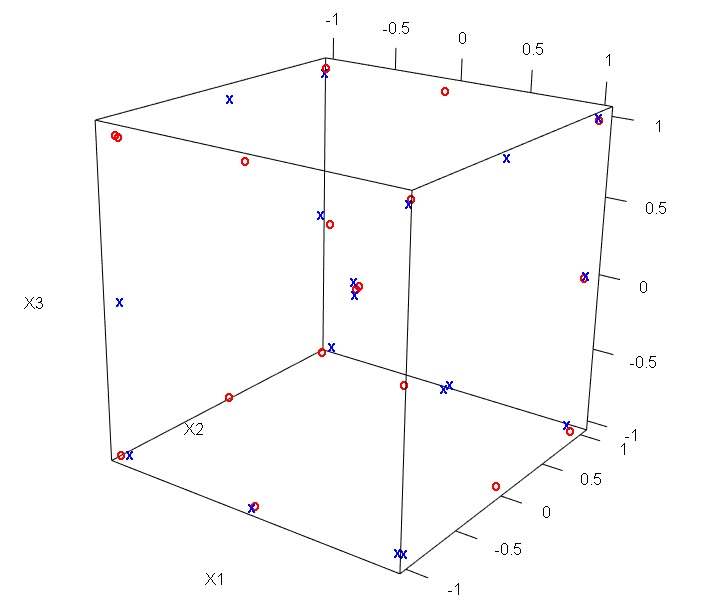
\includegraphics[scale=0.65]{CS_design.jpg}      %width=\textwidth
\caption{MSE(D)-optimal design \#$1$ with two centre points, $\tau^2=1$}
\label{fig::CS_design}
\end{center}
\end{figure} 

Figure \ref{fig::CS_design} provides a graphical representation of the design: the three axes correspond to the experimental factors, each is at three levels (i.e. scaled to $[-1,1]$ dosages): $-1$, $0$ and $1$. Each dot is a design point, and two colours (blue and red) and two symbols (`x' and `o') serve as block indicators. We can see that there are only two centre points in each block, as required, and replicates of other points are generally split between blocks (except for the $(-1,1,1)$ point which is duplicated in the first block only). 

All other designs may be found in the Supplementary material. Time-wise, for the search algorithm's parameters outlined in the beginning of this section, on average an optimal design was found in $13-15$ hours, which was acceptable in this particular case. Sometimes, however, it took up to $20-24$ hours, so some extra time allowance should be accounted for when using these criteria and this search algorithm. 

%%% MSE(D)-optimal designs, WITH centre points: DP, LoF(DPs) and MSE(D) -- LoF as Ds for potential terms
Further we decided to check what designs we would get if there were $5$ levels of each factor rather than $3$, so that all of the third-order terms are estimable (which is also feasible due to a large enough number of runs), i.e. the lack-of-fit component minimising the posterior confidence region for the potential terms would be replaced by the $DP_S$-optimality for them, as in (\ref{eq::crit2}). 

The summary of the corresponding optimal designs is given in Table \ref{tab::MSE(D)_caseCPLoF}: the `new' lack-of-fit component is denoted by DP*s. The notions of `global'  and `local' efficiencies are the same as previously. For each design we calculated its $LoF(DP)$-value, so that we could assess how they would perform in terms of the criterion (\ref{eq::crit1}). The performances of the optimal designs constructed without the restriction of two centre points per block are summarised in Table \ref{tab::MSE(D)_full} in Appendix \ref{app::cs}; all of the designs are also provided in the Supplementary material. In order to illustrate general tendencies in the designs' appearances, designs optimal with respect to the criterion with equal weights, for two values of $\tau^2$ are provided in Table \ref{tab::Full_designs}.

\begin{table}[h]
\centering
\caption{Case-study. Properties of ``Full'' MSE(D)-optimal blocked designs, with two centre points per block}
\label{tab::MSE(D)_caseCPLoF}
\resizebox{\textwidth}{!}}  & \multicolumn{4}{l}{\textbf{`Local' Efficiency,\%}}& \multicolumn{1}{c}{\textbf{Relative}}                          \\
   & \textbf{DP}       & \textbf{DP*s}    & \textbf{MSE(D)}   & \textbf{PE}        & \textbf{LoF}        & \textbf{DP} & \textbf{DP*s}  & \textbf{LoF(DP)}   & \textbf{MSE(D)}  &  \textbf{DP}  &  \textbf{DP*s} & \textbf{LoF(DP)}   & \textbf{MSE(D)} & \textbf{Efficiency,\%} \\
1 & 1/3 & 1/3 & 1/3 & \multicolumn{1}{|r}{14} & \multicolumn{1}{r|}{11} & 80.58 & 69.38 & 87.05 & 91.74 & \multicolumn{1}{|r}{84.46} & 79.90 & 94.36 & \multicolumn{1}{r|}{92.46} & 94.42 \\
2 & 0.4 & 0.2 & 0.4 & \multicolumn{1}{|r}{14} & \multicolumn{1}{r|}{11} & 83.90 & 61.18 & 85.36 & 57.47 & \multicolumn{1}{|r}{87.93} & 70.46 & 92.52 & \multicolumn{1}{r|}{57.92} & 95.83 \\
3 & 0.25 & 0.25 & 0.5 & \multicolumn{1}{|r}{13} & \multicolumn{1}{r|}{12} & 79.93 & 68.24 & 87.06 & 94.05 & \multicolumn{1}{|r}{83.77} & 78.59 & 94.37 & \multicolumn{1}{r|}{94.79} & 96.32 \\
4 & 1 & 0 & 0 & \multicolumn{1}{|r}{20} & \multicolumn{1}{r|}{5} & 95.41 & 0.00 & 62.13 & 95.24 & \multicolumn{1}{|r}{100.00} & 0.00 & 67.34 & \multicolumn{1}{r|}{95.98} & 95.41 \\
5 & 0 & 1 & 0 & \multicolumn{1}{|r}{14} & \multicolumn{1}{r|}{11} & 62.01 & 86.83 & 92.98 & 74.95 & \multicolumn{1}{|r}{64.99} & 100.00 & 100.78 & \multicolumn{1}{r|}{75.53} & 86.83 \\
6 & 0 & 0 & 1 & \multicolumn{1}{|r}{14} & \multicolumn{1}{r|}{11} & 88.31 & 0.00 & 88.35 & 99.23 & \multicolumn{1}{|r}{92.55} & 0.00 & 95.77 & \multicolumn{1}{r|}{100.00} & 99.23 \\
 & & & & & & & & & & & & & & \\
   & \multicolumn{3}{l}{\textbf{Criteria, $\bm{\tau^2=1/q}$}} & \multicolumn{2}{l}{\textbf{DoF}} & \multicolumn{4}{l}{\textbf{`Global' Efficiency,\%}}  & \multicolumn{4}{l}{\textbf{`Local' Efficiency,\%}}& \multicolumn{1}{c}{\textbf{Relative}}                          \\
    & \textbf{DP}       & \textbf{DP*s}    & \textbf{MSE(D)}   & \textbf{PE}   & \textbf{LoF}        & \textbf{DP} & \textbf{DP*s}  & \textbf{LoF(DP)}   & \textbf{MSE(D)}  &  \textbf{DP} & \textbf{DP*s} & \textbf{LoF(DP)}   & \textbf{MSE(D)} & \textbf{Efficiency,\%} \\
1 & 1/3 & 1/3 & 1/3 & \multicolumn{1}{|r}{14} & \multicolumn{1}{r|}{11} & 80.14 & 69.01 & 87.70 & 91.41 & \multicolumn{1}{|r}{83.99} & 81.43 & 90.34 & \multicolumn{1}{r|}{92.07} & 93.97\\
2 & 0.4 & 0.2 & 0.4 & \multicolumn{1}{|r}{14} & \multicolumn{1}{r|}{11} & 83.76 & 61.29 & 88.28 & 94.41 & \multicolumn{1}{|r}{87.79} & 72.31 & 90.95 & \multicolumn{1}{r|}{95.09} & 96.04\\
3 & 0.25 & 0.25 & 0.5 & \multicolumn{1}{|r}{12} & \multicolumn{1}{r|}{13} & 79.66 & 64.43 & 84.44 & 94.84 & \multicolumn{1}{|r}{83.49} & 76.02 & 86.99 & \multicolumn{1}{r|}{95.52} & 95.20\\
4 & 1 & 0 & 0 & \multicolumn{1}{|r}{20} & \multicolumn{1}{r|}{5} & 95.41 & 0.00 & 90.63 & 95.66 & \multicolumn{1}{|r}{100.00} & 0.00 & 93.37 & \multicolumn{1}{r|}{96.35} &  95.41\\
5 & 0 & 1 & 0 & \multicolumn{1}{|r}{14} & \multicolumn{1}{r|}{11} & 59.81 & 84.75 & 86.15 & 72.05 & \multicolumn{1}{|r}{62.68} & 100.00 & 88.75 & \multicolumn{1}{r|}{72.57} & 84.75 \\
6 & 0 & 0 & 1 & \multicolumn{1}{|r}{14} & \multicolumn{1}{r|}{11} & 88.73 & 0.00 & 90.57 & 99.29 & \multicolumn{1}{|r}{92.99} & 0.00 & 93.30 & \multicolumn{1}{r|}{100.00} & 99.29
\end{tabular}
}
\end{table}

\begin{table}[h]
\centering
\caption{Case-study. Designs \#$1$ from Table \ref{tab::MSE(D)_caseCPLoF}, $\tau^2=1$ (left) and $\tau^2=1/q$ (right)}
\begin{center}
\label{tab::Full_designs}
\scalebox{0.73}{
\begin{tabular}{rrrrrrrr|r|rrrrlrrr}
-1 & -1 & 0 &  & -1 & -1 & -1 &  &  &  & -1 & -1 & -1 &  & -1 & -1 & -1 \\
-1 & -1 & 1 &  & -1 & -1 & 0 &  &  &  & -1 & -1 & 0.5 &  & -1 & -1 & 0.5 \\
-1 & 0 & -1 &  & -1 & -1 & 1 &  &  &  & -1 & -0.5 & 1 &  & -1 & -0.5 & 1 \\
-1 & 0.5 & 1 &  & -1 & 0.5 & 1 &  &  &  & -1 & 0 & -0.5 &  & -1 & 1 & -1 \\
-1 & 1 & -1 &  & -1 & 1 & -1 &  &  &  & -1 & 1 & -1 &  & -1 & 1 & 1 \\
-1 & 1 & 0.5 &  & -1 & 1 & 0.5 &  &  &  & -1 & 1 & 1 &  & -0.5 & -1 & -0.5 \\
-0.5 & 1 & 1 &  & -0.5 & -0.5 & 1 &  &  &  & -0.5 & 1 & 0 &  & -0.5 & 0.5 & -1 \\
0 & -1 & -1 &  & -0.5 & 1 & -0.5 &  &  &  & 0 & -1 & 1 &  & 0 & -1 & 1 \\
0 & 0 & 0 &  & 0 & -1 & -1 &  &  &  & 0 & 0 & 0 &  & 0 & 0 & 0 \\
0 & 0 & 0 &  & 0 & 0 & 0 &  &  &  & 0 & 0 & 0 &  & 0 & 0 & 0 \\
0.5 & -1 & 1 &  & 0 & 0 & 0 &  &  &  & 0 & 1 & 1 &  & 0 & 1 & 1 \\
0.5 & 1 & -1 &  & 0.5 & -1 & 1 &  &  &  & 0.5 & -0.5 & -1 &  & 0.5 & 1 & -0.5 \\
1 & -1 & -1 &  & 0.5 & 1 & -1 &  &  &  & 1 & -1 & -1 &  & 1 & -1 & -1 \\
1 & -1 & 0.5 &  & 1 & -1 & -1 &  &  &  & 1 & -1 & 0 &  & \textbf{1} & \textbf{-1} & \textbf{1} \\
1 & -0.5 & 1 &  & 1 & -1 & 0.5 &  &  &  & 1 & 0.5 & 1 &  & \textbf{1} & \textbf{-1} & \textbf{1} \\
1 & 0.5 & -1 &  & 1 & -0.5 & -0.5 &  &  &  & \textbf{1} & \textbf{1} & \textbf{-1} &  & 1 & 0 & -0.5 \\
1 & 1 & -0.5 &  & 1 & 0.5 & -1 &  &  &  & \textbf{1} & \textbf{1} & \textbf{-1} &  & 1 & 0.5 & 1 \\
1 & 1 & 1 &  & 1 & 1 & 1 &  &  &  & 1 & 1 & 0.5 &  & 1 & 1 & 0.5
\end{tabular}
}
\end{center}
\end{table}

In case of $\tau^2=1$ all pure error degrees of freedom (except for the $2$ coming from the replicated centre points) occur from $12$ points duplicated in different blocks; in case of $\tau^2=1/q$ (i.e. $\tau^2=0.1$) two `corner' points are replicated within the same block (they are highlighted in Table \ref{tab::Full_designs}). Quite a few experimental units would receive an `intermediate' $\pm 0.5$ dosage of at least one product, and as this did not comply with the demands of the experimenters, the choice was still made in favour of the three-level design in Table \ref{tab::CS_Design}. 

%% Discussion points
\section{Conclusions}

In general, this chapter is about exploring the flexibility of the design optimality criteria and implementation introduced previously. We adapted the approach to the framework of a blocked experiment, and by considering an example confirmed some of the key features of the relationships between the individual components, and tendencies in optimal designs obtained with various weight allocation schemes. Due to the relatively high time consumption of the determinant-case criterion calculation, the simplest suggested alternative seemed quite promising in terms of providing adequate designs in a much more reasonable time.

The second part of the chapter is devoted to a real-life design problem, such that the given framework of a blocked factorial experiment with some suspicion regarding possible model disturbance suggested applying the MSE-based criterion for the design construction. In addition, the structure of the criterion and the search algorithm implementation allowed for necessary adaptation with regard to the pre-specified restrictions, so that a set of possible solutions was presented satisfying the objectives of the particular experiment. 

  

\chapter{MSE-based Criteria for Multistratum Experiments}
\label{ch::mse_ms}
 %%% Multi-stratum designs, MSE-criteria
In this chapter we will adapt the MSE-based criteria derived before to the factorial experiments with units distributed in several strata. First we shall briefly review the approaches to the inference from the experiments with multi-level unit structures, and then will define the MSE-based optimality for the multistratum framework and provide the implementation strategy for the corresponding design search.

In Section \ref{sec::ch7_ex} a few illustrative examples will be considered, for the main purposes of assessing the obtained optimal designs' performances and structures, and investigating the presence of any patterns and tendencies regarding the relationships between the criteria form, parameters and the results. 

\section{Response-Surface Methodology for Multistratum Designs}
%% Model. Ratio of variances.
As randomisation occurs at each stratum, the model accounting for the hierarchical error structure and correlated observations can be written as
\begin{equation}
\label{eq::MS_model}
\bm{Y}=\bm{X}\bm{\beta}+\sum_{i=1}^{s}\bm{Z}_{i}\bm{\varepsilon}_{i},
\end{equation}
where $\bm{Y}$ represents the $n$-dimensional vector of responses, $\bm{X}$ stands for the $n \times p$ model matrix and $\bm{\beta}$ for the $p$-dimensional vector of corresponding model coefficients. Each row of the $n\times m_{i}$ matrix $\bm{Z}_{i}$ corresponds to a single experimental run and indicates the unit in stratum $i$ containing this run. $\bm{\varepsilon}_{i}$ is a vector of random effects occurring due to the randomisation at level $i$, and these effects are assumed to be independent and identically distributed around zero mean and variance $\sigma^{2}_{i}$. The assumption of error normality, though quite common is required for some analysis methods, is not a necessary one at this stage.

The majority of purposes of inference rely on obtaining parameter estimates $\bm{\hat{\beta}}$ of good quality, that is minimising the uncertainty of the obtained estimates, which implies the necessity of evaluating the dispersion parameters $\sigma^2_{i}$ that are directly related to the estimates' variance and, therefore, responsible for measuring the uncertainty of the inference in a general sense.

\section{REML Methodology}
An extensive amount of research has been conducted on the design of and analysis of data from split-plot and split-split-plot experiments, with one of the first works by \cite{Letsinger1996BiRandomization}, emphasising the necessity of adapting the design and analysis strategy with respect to the more complicated error structure.  In the most general case of non-orthogonal unit structures Residual Maximum Likelihood (REML) methodology has been acknowledged to be the most sensible approach to estimating the variance components by maximising the part of the likelihood function corresponding to the ``random'' part of the model; the details are provided, for example, in \cite{Searle2001generalized}. 

In traditional REML-based methodology the estimates of $\sigma^{2}_{i}$ are obtained from model (\ref{eq::MS_model}) and then GLS estimators of $\bm{\beta}$ are calculated as
\begin{equation}
\label{eq::MS_GLS}
\bm{\hat{\beta}}=(\bm{X}'\bm{V}^{-1}\bm{X})^{-1}\bm{X}'\bm{V}^{-1}\bm{Y},
\end{equation}
where $\bm{V}$ is the unknown variance-covariance matrix of the response vector, to which the estimates are to be plugged in:
\begin{equation*}
\bm{V}=\sum_{i=1}^{s}\sigma^{2}_{i}\bm{Z}_{i}\bm{Z}'_{i},
\end{equation*}
so that $\mbox{Var}(\bm{\hat{\beta}})=(\bm{X}'\bm{V}^{-1}\bm{X})^{-1}.$

However, in some cases REML tends to underestimate the variance components in the higher stratum, for example \cite{Goos2006practical} considered some split-plot experiments with true whole-plot variances being non-negligibly far from zero, for which REML, however, provided zero estimates. 

A possible alternative would be a Bayesian analysis, that is specifying prior information regarding the variance components (as was suggested by \cite{Gilmour2009analysis}), however, this requires a careful choice of the prior which is often not possible, especially in the case of more than two strata.

\section{Full Treatment Model}

In the context of model uncertainty it would be appropriate to loosen the assumption of the response surface model (\ref{eq::MS_model}) and consider instead the relationship of the response with the set of treatments:
\begin{equation}
\label{eq::treatmentMS}
\bm{Y}=\bm{X_t}\bm{\tau}+\sum_{i=1}^{s}\bm{Z}_{i}\bm{\varepsilon}_{i}.
\end{equation}

Each column of $\bm{X_t}$ here corresponds to a treatment defined as a combination of the experimental factors;
%in case of factorial experiment the total number of possible treatments (or candidate design points) $T$ would be the product of the number of the factors' levels. 
$\bm{Z}_{i}$, as before, is the indicator matrix of random effects at stratum $i$.

\subsection{Pure-error REML}
\cite{GilmourGoos2016PEREML} introduced the notion of ``Pure Error REML'', such that the random effects are estimated from the treatment model (\ref{eq::treatmentMS}), and then for the sake of making inference regarding parameters of the response model (\ref{eq::MS_model}), they are substituted in the GLS estimators of the fixed effects (\ref{eq::MS_GLS}). It is also argued that some appropriate corrections are to be adapted and applied to the obtained estimates, i.e.~the ones suggested by \cite{kenward1997small}. 

A careful definition of ``pure error'' is necessary when considering the treatment and response surface models, especially in the presence of nested random block effects. \cite{Gilmour2000PErsm} discuss the pure error estimation issues in the context of blocked experiments. 

Pure error is expected to measure the variability between experimental units regardless of the treatments applied, and therefore, the assumption of treatment-unit additivity is essential in unblocked experiments.  In the presence of one or several blocking factors, the existence of block-treatment interaction would imply that pure error in the lower strata can only be estimated from the replicates within blocks, so that inter-block information is not taken into consideration. Hence, in the blocked cases the assumption of treatment-block additivity \citep{Draper1998} is desirable. \cite{Gilmour2000PErsm} argue for the preservation of treatment-unit additivity when either fixed or random block effects are in the model in order to preserve consistency with the unblocked experiments; that would also conveniently imply treatment-block additivity. Adoption of these assumptions would then lead to the following representation of the relationship between responses and treatments in multi-stratum experiments. 

The outcome of applying treatment $i$ $(i=1\ldots T)$ to the experimental run located in the units $j_1$ of the first stratum, $j_2$ of the second stratum, $\ldots$ , and unit $j_s$ of the $s-$th stratum can be expressed as follows:
\begin{equation}
\label{eq::ms_tr}
y_{ij_{1}...j_{s}}=\mu+t_{i}+b_{j_1}+\ldots +b_{j_s},
\end{equation}
where $b_{j_s}$ is usually denoted as between-run variation. 

Under the stronger assumption of the response surface model (\ref{eq::MS_model}), the treatment effects $t_{i}$ are represented as a set of polynomial model terms.  

Based on the interrelation of the two models, and the desirability of being able to provide the possibility for testing for the lack-of-fit together with obtaining robust estimates of the variance components, the approach of using pure error is adopted, \cite{GilmourGoos2016Robust} explored several approaches to estimating the variance components. 

\subsection{Yates' procedure}
\label{sec::ch7_varest}
The first approach is stratum-by-stratum data analysis, where each randomisation level is considered separately, and at each stratum $i$ units are treated as runs aggregated in $m_{i-1}$ blocks with fixed effects. The lower stratum variance is estimated from within blocks (using intra-block residual mean square), and the higher stratum (inter-block) variance from the difference between the intra- and inter-block residual mean squares scaled by the number of runs per block \citep{Hinkelmann2005Advanced}. This simple strategy requires no other assumptions except for the treatment-unit additivity and provides unbiased treatment effects' estimators.

However, as mentioned before, it would be desirable to make use of combining inter- and intra-block information, especially in the common cases of relatively small experiments when the amount of runs available does not allow for obtaining higher stratum variance components from only considering blocks as whole units. Yates' procedure, first suggested by \cite{yates1939recovery} and described in detail by \cite{Hinkelmann2005Advanced}, provides more degrees of freedom for the variance estimate in the higher stratum. 

Within-block variance is obtained from the residual mean square, as before. The between-block variation is estimated form fitting the block-after-treatment model: the treatment sum of squares  accounted for the blocks corresponding to the higher strata and the residual sum of squares obtained in the intra-block analysis are subtracted from the total sum of squares. What remains is the extra sum of squares for the blocks in the current stratum, which is used for estimating the intra-block variation.
%Whereas between-block variation is estimated from what is left for the blocking components sum of squares in the current stratum after the sums of squares corresponding to the block effects of the higher strata and all treatments are subtracted from the total sum of squares accounted for the residual sum of squares. 
Schematically these two steps can be presented as below (with the order of the components being crucial):
\begin{enumerate}
\item Total SS = SS(Blocks) + SS(Treatments$\vert$Blocks) + SS(Residual)\\
From fitting this full treatment-after-blocks model the residual mean square $S^2$ is taken as the estimate of the intra-block variance. SS(Residual) is then substituted in the following partition.
\item Total SS = SS(Treatments) + SS(Blocks$\vert$Treatments) + SS(Residual)\\
Therefore, the sums of squares for the blocks after the treatment effects have been accounted for is obtained and the corresponding mean square $$S^2_{b}=\mbox{SS(Blocks$\vert$Treatments)}/\nu_{b}$$ is then used to get an estimate of the inter-block variance:
\item $\hat{\sigma}^2_{b}=\frac{\nu_{b}(S^2_{b}-S^2)}{d}$,\\
where $d=n-\mbox{trace}[\bm{Z}'\bm{X_t}(\bm{X_t}'\bm{X_t})^{-1}\bm{X_t}'\bm{Z}]$, $\nu_{b}=\mbox{rank}([\bm{X_t} \bm{Z}])-\mbox{rank}(\bm{X_t})$, and $\bm{X_t}$ and $\bm{Z}$ are as in (\ref{eq::treatmentMS}).
\end{enumerate}

\cite{GilmourGoos2016Robust} show that in addition to the treatment-unit additivity and randomisation the assumption of the experimental units being a random sample from an infinite population is necessary for the inter-block variance estimate to be unbiased. In this particular context, when the normality and independence of responses in (\ref{eq::MS_model}) is a standard assumption, although a potential presence of contamination effects in the fixed part of the model is also accounted for, Yates' approach seems to be the most appropriate technique. However, relying on the distribution assumption to the extent that makes REML the most sensible approach means that the fixed part of the fitted model is assumed to be absolutely true, that is the parameters of the population distribution are known, which does not comply with the model uncertainty framework. 

Together with the specifications regarding estimation of the variance components, it is necessary to carefully establish the way the pure error degrees of freedom should be determined and how the available remaining number of treatment degrees of freedom would be distributed between the polynomial, lack-of-fit and inter-block information components. 

\section{Design Construction for MSE-based Optimality Criteria}
\label{sec::ch7_search}
With the theoretical insights discussed above in mind, the practical adaptation and implementation of the MSE-based criteria for multistratum experiments shall be presented as the algorithm of the corresponding optimal design search which is in accordance with the inference strategy described in the previous section.

Recall the general outline of a multistratum experiment (as in Section \ref{sec::back_ms}): 
\begin{itemize}
\item There are $s$ strata nested within each other, stratum number $0$ denoting the whole experiment. A higher stratum number corresponds to the lower level in the hierarchical unit structure.
\item Every unit at stratum $i-1$ contains $n_i$ units at the lower stratum $i$, so that stratum $j$ contains $m_j=\prod_{i=1}^{j}n_{i}$ units and in total there are $n=m_{s}=\prod_{i=1}^{s}n_{i}$ runs. 
\item At least one factor is applied at some of the strata, if there is a stratum with no factor applied, then at this level only blocking is accounted for.
\end{itemize}

In the presence of potential model disturbance which is expressed as a matrix of polynomial terms, the full model for a multistratum experiment is then:
\begin{equation}
\label{eq::MS_model_full}
\bm{Y}=\bm{X}_1\bm{\beta}_1+\bm{X}_2\bm{\beta}_2+\sum_{i=1}^{s}\bm{Z}_{i}\bm{\varepsilon}_{i},
\end{equation}
where $\bm{X}_1$ is the primary terms matrix, which was denoted as $\bm{X}$ in the fitted model (\ref{eq::MS_model}). 

\subsection{Construction procedure}
The design construction will follow the approach developed by \cite{Trinca2015improved}: an iterative, stratum-by-stratum algorithm, that treats the higher stratum units as fixed blocks; such an approach does not require any prior assumptions regarding the values of the variance components. 

At each step a candidate set of treatments applied at the current stratum is to be generated, and the point exchange algorithm is applied. The model matrix to be used in the optimisation comprises model terms from all higher strata (with the factor values for individual runs obtained at previous steps), terms from the current stratum and interactions between these two groups of terms, if there are any to be considered. The allocation of the degrees of freedom shall be implemented according to the Yates procedure, and some illustrative examples will be given later on.

Before moving to a more detailed presentation of the design construction algorithm, recall the MSE-based criteria (\ref{eq::MSE_D}), (\ref{eq::MSE_L}), (\ref{eq::MSE_D_B}) and (\ref{eq::MSE_L_B}) that are to be used:

For an unblocked experiment:
\begin{itemize}
\item Determinant-based $MSE(D)$ criterion:
\begin{align}
\label{eq::MSE_D_ms}
\mbox{minimise }&\left[\left|\bm{X}'_{1}\bm{X}_{1}\right|^{-1/p}F_{p,d;1-\alpha_{DP}}\right]^{\kappa_{DP}} \times \notag \\ &\left[\left|\bm{L}+\frac{\bm{I}_{q}}{\tau^{2}}\right|^{-1/q}F_{q,d;1-\alpha_{LoF}}\right]^{\kappa_{LoF}}\times \notag\\ & \left[|\bm{X}'_{1}\bm{X}_{1}|^{-1}\exp\left(\frac{1}{N}\sum_{i=1}^{N}\log(1+\bm{\tilde{\beta}}_{2i}'\bm{X}_2^{'}\bm{X}_1\bm{M}^{-1}\bm{X}_1^{'}\bm{X}_2\bm{\tilde{\beta}}_{2i})\right)\right]_{.}^{\kappa_{MSE}/p}
\end{align}
\item Trace-based $MSE(L)$ criterion:
\begin{align}
\label{eq::MSE_L_ms}
\mbox{minimise} &\left[\frac{1}{p}\mbox{trace}(\bm{WX}'_{1}\bm{X}_{1})^{-1}F_{1,d;1-\alpha_{LP}}\right]^{\kappa_{LP}}\times \notag\\& \left[\frac{1}{q}\mbox{trace}\left(\bm{L}+\frac{\bm{I}_{q}}{\tau^{2}}\right)^{-1}F_{1,d;1-\alpha_{LoF}}\right]^{\kappa_{LoF}}\times 
\notag\\& \left[\frac{1}{p}\mbox{trace}\{(\bm{X}'_{1}\bm{X}_{1})^{-1}+\tau^2\bm{A}\bm{A}'\}\right]^{\kappa_{MSE}}_{.}
\end{align}
\end{itemize} 
 
For a blocked experiment:
\begin{itemize}
\item Determinant-based $MSE(D)$ criterion:
\begin{align}
\label{eq::MSE_D_B_ms}
\mbox{minimise }&\left[\left|(\bm{X}'_{1}\bm{Q}\bm{X}_{1})^{-1}\right|^{1/p}F_{p,d_B;1-\alpha_{DP}}\right]^{\kappa_{DP}} \times \notag \\ &\left[\left|\bm{\tilde{L}}+\frac{\bm{I}_{q}}{\tau^{2}}\right|^{-1/q}F_{q,d_B;1-\alpha_{LoF}}\right]^{\kappa_{LoF}}\times \notag\\ & \left[|\bm{X}'_{1}\bm{QX}_{1}|^{-1}\exp\left(\frac{1}{N}\sum_{i=1}^{N}\log(1+\bm{\tilde{\beta}}_{2i}'\bm{X}_2^{'}\bm{QX}_1\bm{\tilde{M}}^{-1}\bm{X}_1^{'}\bm{QX}_2\bm{\tilde{\beta}}_{2i})\right)\right]_{.}^{\kappa_{MSE}/p}
\end{align}
\item Trace-based $MSE(L)$ criterion:
\begin{align}
\label{eq::MSE_L_B_ms}
\mbox{minimise }&\left[\frac{1}{p}\mbox{trace}(\bm{WX}'_{1}\bm{Q}\bm{X}_{1})^{-1}F_{1,d_B;1-\alpha_{LP}}\right]^{\kappa_{LP}}\times \notag \\&\left[\frac{1}{q}\mbox{trace}\left(\bm{\tilde{L}}+\frac{\bm{I}_{q}}{\tau^{2}}\right)^{-1}F_{1,d_B;1-\alpha_{LoF}}\right]^{\kappa_{LoF}}\times \notag \\& \left[\frac{1}{p}\mbox{trace}\{(\bm{X}'_{1}\bm{QX}_{1})^{-1}+\tau^2[\bm{\tilde{A}}\bm{\tilde{A}}']_{22}\}\right]^{\kappa_{MSE}}_{.}
\end{align}
\end{itemize} 

Then the optimal multistratum design search is implemented following the steps below:
\begin{enumerate}
\item Starting from the first stratum, if there are any factors applied at this level, a candidate set of treatments is formed together with the fitted model matrix comprising the primary terms and the matrix of potential terms. The optimal unblocked design $X_1$ is then obtained using the usual point-exchange algorithm, by minimising (\ref{eq::MSE_D_ms}) or (\ref{eq::MSE_L_ms}). The labels of the treatments applied at the current stratum are saved at this stage as well in order to calculate the number of pure error degrees of freedom at the lower strata.

If there are no factors applied at the first stratum, we move to the second one, and conduct the optimal design search for a blocked experiment, where the number of blocks is equal to the number of units in the first stratum $n_1$, with $n_2$ runs per block; in this case criterion function (\ref{eq::MSE_D_B_ms}) or (\ref{eq::MSE_L_B_ms}) is used, and number of pure error degrees of freedom $d_B$ is calculated according to the usual blocked experiment framework. Treatment labels are saved as well. 
 
\item When moving from stratum $i-1$ to stratum $i$, all factors applied in the higher strata are now treated as ``whole-plot'' factors. The corresponding model matrix $\bm{Xw.m}$ containing terms inherited from the higher strata is expanded accordingly, as treatments applied at each unit in stratum $i-1$ are now applied to $n_i$ units of the current stratum nested within it. A similar expansion procedure is carried out for the vector (or matrix, if there are two or more higher strata with factors applied) of the treatment labels, so that for each current unit we are able to see what treatment has been applied to it at each stratum.

Blocking with no factors applied may occur at any stratum, not only at the first one. In such cases the procedure remains the same: skipping to the next stratum with some treatment applied, expanding the design matrices and vectors with treatment labels corresponding to the higher strata.

\item Once there is a model matrix with the ``whole-plot'' terms is formed, the search procedure might be started for the current stratum. The candidate set of treatments is set for the factors applied in the current stratum; parameters of interest include not only the ones formed by these factors but also their interactions with the higher strata terms. As nesting within the previous strata is treated as fixed block effects, the criteria used are the ones given in (\ref{eq::MSE_D_B_ms}) and (\ref{eq::MSE_L_B_ms}). However, there are a few features worth noting:
\begin{itemize}
\item For each design under consideration during the extensive search procedure, its model matrix $\bm{X}_1$ is now constructed by binding the ``whole-plot'' model matrix $\bm{Xw.m}$, the model comprising the terms formed from the factors applied at the current stratum $\bm{Xi.m}$, and the matrix formed of the interaction terms (if any are to be included) between the two. The same relates to the construction of the potential terms matrix $\bm{X}_2$: it needs to be recalculated every time a design point is swapped between the candidate set of the current stratum terms and the current design if it contains any interactions involving terms inherited from the previous strata. If not, it then only comprises terms from the current stratum factors.
\item Presence of the potential terms matrix in the criteria also implies that each stratum $i$ will ``have'' its own number of potential terms $q_i$ and, therefore, in the cases when the value of the variance scaling parameter $\tau^2$ depends on it, at each stratum the criterion function will be evaluated with the respective values of $\tau^2_i$ instead of some common one for all levels. In this work we consider common values of $\tau^2$, however, it is a case-sensitive parameter, and it is to be discussed in each particular case.
\item As the numbers of primary and potential terms vary from stratum to stratum, so do the significance levels $\alpha_{LP}$ and $\alpha_{LoF}$ in the case of trace-based criterion (\ref{eq::MSE_L_B_ms}):
\begin{align*}
\alpha_{LP}&=1-(1-\alpha_1)^{\frac{1}{p}},\\
\alpha_{LoF}&=1-(1-\alpha_2)^{\frac{1}{q}},
\end{align*}
as the corrected confidence levels depend on the dimension of the confidence regions (as in (\ref{eq::Sidak})). 
\item We use the same values of weights in the criteria for all strata; however, the flexibility of the algorithm allows changing weights (and even criteria) between the strata.
\end{itemize}
\item If there are at least $3$ strata with some factors applied, and when the current stratum number is $3$ or more, an additional swapping procedure is performed (the same as that described by \cite{Trinca2001multistratum}). By looking at the $i-2$ stratum units that have the same treatments applied to them, and interchange the $i-1$ stratum units within those, the performance of the design evaluated with respect to the performance at the current stratum $i$. The same swapping is performed for all the higher strata up to the first one.
\item It is all then repeated from step number $2$, until current stratum $i$ reaches the lowest stratum $s$. 
\end{enumerate}

\subsection{Allocation of degrees of freedom}

The distribution of the degrees of freedom among different components at each stratum of the resulting design needs to be evaluated in accordance with the variance estimation procedure (as described in Section \ref{sec::ch7_varest}), so that both intra- and inter-block information is taken into account. 

We shall consider here the case of a split-split-plot experiment (i.e. with $3$ strata), but this strategy is straightforwardly extended to the cases with any number of randomisation levels. At the first $2$ strata, where experimental units are to be further expanded, and treatments applied at these levels are to be replicated for all sub-units and runs within then the available degrees of freedom (after fitting the model at this current level) are split between three components: pure error, inter-plot (inter-whole-plot and inter-sub-plot for the $1$st and $2$nd strata respectively) and lack-of-fit. In the lowest stratum there are, as in the unblocked cases and experiments with fixed block effects, only pure error and lack-of-fit components.

Starting with presenting the way of calculating the number of pure error degrees of freedom at each level, we then proceed to the details of the inter-plot and lack-of-fit degrees of freedom evaluation accompanied by the corresponding R code. In the end of this section we will consider an illustrative example of a design and see how degrees of freedom are allocated.

If we consider an experiment with $n_1$ units in the first stratum, with each of them having $n_2$ units of stratum $2$, and with $n_3$ runs nested within each of those, there are $n=n_1\times n_2\times n_3$ runs in total. The notation to be used is as follows:
\begin{itemize}
\item $\bm{y}$ -- an $n$-dimensional dummy response vector (any randomly generated vector), which is used for fitting a linear model;
\item $\bm{B_1}$ -- an $n$-dimensional vector, such that its $i$-th element is the label of the first stratum unit that contains the $i$-th run. Similarly, $\bm{B_2}$ contains labels of the second stratum units;
\item  $\bm{T_{W}}$ -- a vector of labels for treatments applied at the first stratum (whole-plots); $\bm{T_{S}}$ -- a vector of labels for treatments applied at the second stratum units (sub-plots); this includes treatments in the higher stratum. And, finally, $\bm{T_{SS}}$ contains labels for all treatments applied at the lowest stratum, i.e. at individual runs;
\item $\bm{Xw.m}$, $\bm{Xs.m}$ and $\bm{Xss.m}$ are the matrices containing fixed model terms that are to be fitted at the $1$st, $2$nd and $3$rd strata respectively.
\end{itemize}

If we denote by $p_i$ the number of the fixed model terms fitted at the $i$-th stratum, then the number of available degrees of freedom at each level is: $n_1-1-p_1$ for the $1$st, $n_1\times(n_2-1)-p_2$ -- for the $2$nd, and $n_1\times n_2\times(n_3-1)-p_3$ -- for the $3$rd stratum.

After a design has been obtained, and all the treatment labels, block indicators and model matrices are in place, fitting the following linear models and studying their summary (i.e.~ANOVA) will provide the numbers of degrees of freedom corresponding to every component. 

We start with fitting the full treatment model schematically presented in (\ref{eq::model_pe}): the effects of treatments applied to all strata, followed by the terms containing strata indicators, `$\bm{B_i}$'. In the resulting summary we then will see the distribution of pure error degrees of freedom: in the row corresponding to `$\bm{B_1}$' for the whole-plots ($1$st stratum), and in the row corresponding to `$\bm{B_2}$' for the sub-plots ($2$nd stratum). The `Residual' number of degrees of freedom is equal to the number of pure error degrees of freedom for the $3$rd stratum.
\begin{equation}
\label{eq::model_pe}
\mathrm{lm}(\bm{y}\sim\bm{T_{SS}}+\bm{B_1}+\bm{B_2}).
\end{equation}
The order of terms in the expression above is crucial: this is a block-after-treatment model fitting; and the pure error degrees of freedom for lower-level plots occur not only when they are replicated within the same higher-level plot, but also when some pairs of treatments are split between two (or more) higher-level plots. An example of a design is given at the end of this section together with a detailed description of how each pure error degree of freedom is obtained.

From the summary of model (\ref{eq::model_pe}) we automatically obtain the number of lack-of-fit degrees of freedom (LoF) for the lowest stratum, as $n_1\times n_2\times(n_3-1)-p_3 = $`Residual' P.E. $+$ LoF.

Now we need to evaluate the number of degrees of freedom for estimating the inter-whole-plot/inter-sub-plot and lack-of-fit components for the first two strata. For this purpose, at each of the higher strata, we fit a linear model comprising polynomial terms (formed of the factors applied at the current and all higher strata), treatment labels, and current and all higher strata unit indicators. By doing so and first projecting the vector of (dummy) responses to the subspaces generated by the parametric model's terms and by the treatments, we account for the degrees of freedom required for evaluating the model parameters' estimates and for the lack-of-fit degrees of freedom. The number of degrees of freedom left for the components corresponding to the current stratum indicators is the sum of the inter-whole-plot (inter-sub-plot) and pure error degrees of freedom. 
\begin{align}
\label{eq::model_lof1}
&\mathrm{lm}(\bm{y}\sim\bm{Xw.m}+\bm{T_{W}}+\bm{B_1}),\\
\label{eq::model_lof2}
&\mathrm{lm}(\bm{y}\sim\bm{Xw.m}+\bm{Xs.m}+\bm{T_{S}}+\bm{B_1}+\bm{B_2}).
\end{align}
Therefore, the summary of the model in (\ref{eq::model_lof1}) provides the sum of inter-whole-plot and pure error degrees of freedom under the `$\bm{B_1}$' component; and the `$\bm{B_2}$' component of the the summary of (\ref{eq::model_lof2}) gives the same sum for the sub-plot level. Hence, by substituting the number of pure error degrees of freedom, we obtain the inter-whole-plot/inter-sub-plot and then, from the known total numbers, -- the lack-of-fit degrees of freedom for the first and seconds strata.  

In Table \ref{tab::SSP_design} below an example of a split-split-plot design is provided, with $12$ whole-plots, each containing $2$ sub-plots of size $2$, i.e. 48 runs in total. 
\begin{table}[h]
\centering
\caption{Split-split-plot design}
\label{tab::SSP_design}
\scalebox{0.85}{
\begin{tabular}{r|rr|r|rr|rr|rr|r|rr|}  
\cline{2-6} \cline{9-13}
I   & -1 & -1 & -1 & -1 & -1 & & VII  & 0 & 0  & -1 & 1  & 0  \\
    & -1 & -1 & -1 & 1  & 1  & &      & 0 & 0  & -1 & 0  & 0  \\ \cline{4-6} \cline{11-13}
    & -1 & -1 & 1  & -1 & 1  & &     & 0 & 0  & -1 & 1  & 0  \\
    & -1 & -1 & 1  & 1  & 1  & &      & 0 & 0  & -1 & 0  & 0  \\ \cline{2-6} \cline{9-13}
    &    &    &    &    &    & &      &   &    &    &    &    \\ \cline{2-6} \cline{9-13}
II  & -1 & -1 & -1 & -1 & -1 & & VIII & 0 & 1  & 0  & 1  & 0  \\
    & -1 & -1 & -1 & 1  & 1  & &      & 0 & 1  & 0  & 1  & 0  \\\cline{4-6} \cline{11-13}
    & -1 & -1 & 1  & -1 & 1  & &      & 0 & 1  & -1 & 1  & 1  \\
    & -1 & -1 & 1  & 1  & 1  & &      & 0 & 1  & -1 & -1 & 0  \\  \cline{2-6} \cline{9-13}
    &    &    &    &    &    & &      &   &    &    &    &    \\ \cline{2-6} \cline{9-13}
III & -1 & 0  & 1  & 0  & -1 & & IX   & 1 & -1 & 1  & 1  & 1  \\
    & -1 & 0  & 1  & 1  & 0  & &      & 1 & -1 & 1  & -1 & -1 \\\cline{4-6} \cline{11-13}
    & -1 & 0  & 1  & 0  & -1 & &      & 1 & -1 & -1 & 0  & 1  \\
    & -1 & 0  & 1  & 1  & 0  & &      & 1 & -1 & -1 & 0  & 1  \\  \cline{2-6} \cline{9-13}
    &    &    &    &    &    &  &     &   &    &    &    &    \\ \cline{2-6} \cline{9-13}
IV  & -1 & 1  & 0  & -1 & 1  & & X    & 1 & -1 & 1  & -1 & 1  \\
    & -1 & 1  & 0  & 1  & -1 & &      & 1 & -1 & 1  & 1  & -1 \\\cline{4-6} \cline{11-13}
    & -1 & 1  & 1  & -1 & -1 & &      & 1 & -1 & -1 & 0  & 0  \\
    & -1 & 1  & 1  & 0  & 1  & &      & 1 & -1 & -1 & 0  & 0  \\  \cline{2-6} \cline{9-13}
    &    &    &    &    &    & &      &   &    &    &    &    \\ \cline{2-6} \cline{9-13}
V   & -1 & 1  & 0  & -1 & 1  & & XI   & 1 & 0  & -1 & -1 & -1 \\
    & -1 & 1  & 0  & 1  & -1 & &      & 1 & 0  & -1 & 1  & 0  \\\cline{4-6} \cline{11-13}
    & -1 & 1  & 1  & -1 & -1 & &      & 1 & 0  & -1 & -1 & -1 \\
    & -1 & 1  & 1  & 0  & 1  & &      & 1 & 0  & -1 & 1  & 0  \\ \cline{2-6} \cline{9-13}
    &    &    &    &    &    & &      &   &    &    &    &    \\ \cline{2-6} \cline{9-13}
VI  & 0  & -1 & -1 & -1 & 0  & & XII  & 1 & 1  & 1  & -1 & 0  \\
    & 0  & -1 & -1 & 1  & -1 & &      & 1 & 1  & 1  & 1  & -1 \\ \cline{4-6} \cline{11-13}
    & 0  & -1 & -1 & -1 & 0  & &      & 1 & 1  & -1 & 0  & -1 \\
    & 0  & -1 & -1 & 1  & -1 & &      & 1 & 1  & -1 & -1 & 1  \\ \cline{2-6} \cline{9-13}
\end{tabular}
}
\end{table}    

We see that whole-plots I and II, and IV and V are identical, but with the sub-plot and sub-sub-plot treatments being different, so each such replicate provides $1$ whole-plot (WP), $1$ sub-plot(SP) and $2$ sub-sub-plot (SSP) pure error degrees of freedom. Whole-plots III, VI, VII and XI contain replicated sub-plots, although the sub-sub-plot treatments are not replicated within each sub-plot. Therefore, each of them provides $1$ SP and $1$ SSP pure error degree of freedom. 

Finally, whole-plots VIII, IX and X contain $1$ replicated point (SSP treatment) within one of the sub-plots, which provides another $3$ SSP pure error degrees of freedom. In total, for three strata, there are $2$, $6$ and $11$ pure error degrees of freedom respectively.

This particular design was obtained according to one of the MSE(D)-optimality criteria, and its summary is presented in Table \ref{tab::mseD_ex2} (design \#$5$ for $\tau^2=1/q$); the outline of the experimental framework is given in detail in the next Section.

\section{Examples}
\label{sec::ch7_ex}
%%% Examples of MSE MS optimal desgins. 

In this section we shall consider three illustrative examples of multistratum experiments, with $2$, $3$ and $4$ strata. By implementing the stratum-by-stratum design search algorithm presented above, we will obtain determinant- and trace-based MSE-optimal designs. The third component in the MSE(D) criterion is estimated using the Monte-Carlo approach as given in Chapter \ref{ch::mse}; the point prior estimates are not considered here mainly because the results were obtained with the normal prior in a very reasonable time and there was no need for an alternative. 

All the designs will be obtained using three values of the variance scaling parameter $\tau^2$, that is $1$, $1/q$ and $\sqrt{1/q}$, where $q$ stands for the total number of potential terms in the full model (\ref{eq::MS_model_full}). As this number tends to become quite large once the experiment is not too small, the value of $\tau^2=\sqrt{1/q}$ would provide an intermediate value between $1/q$ (which can be very small) and $1$. We shall assess designs' performances in terms of individual criteria for the model parameters in the lowest stratum, and see how available degrees of freedom are allocated between the pure error, inter-block information and lack-of-fit components at each stratum. 

%% Example 1: 
\subsection{Example 1}

In the first example a $2$-stratum experimental framework is considered, with $2$ and $3$ three-level factors applied respectively; the first stratum has $18$ whole-plots with $3$ sub-plots in each, i.e. $54$ experimental runs in total. The full quadratic polynomial model is to be fitted, with $5$ parameters in the highest stratum ($2$ linear, $2$ quadratic and $1$ interaction term) and $15$ in the lowest one ($3$ of each of linear, quadratic and interaction terms plus $6$ interaction terms with the factors applied in the first stratum).

Regarding the third-order potential terms, there are $2$ of them in the first stratum and $28$ in the second, $30$ in total; therefore, the values of $\tau^2$ used are $1/q\approx 0.033$, $\sqrt{1/q}\approx 0.18$ and $1$.

The $MSE(D)$-optimal designs obtained are summarised in Table \ref{tab::mseD_ex1}: the three parts correspond to different values of $\tau^2$; the columns after those containing the weight allocation present the degrees of freedom distribution: the first three correspond to the first stratum (pure error, inter-whole-plot and lack-of-fit components), and the following two -- to the second stratum (pure error and lack-of-fit). A similar structure holds for the $MSE(L)$-optimal designs presentation in Table \ref{tab::mseL_ex1}.

\begin{table}[h]
\centering
\caption{Example 1. Properties of MSE(D)-optimal designs}
\label{tab::mseD_ex1}
\scalebox{0.7}{
\begin{tabular}{rrrrcccrrrrr}
 & \multicolumn{3}{l}{\textbf{Criteria, $\bm{\tau^2=1/q}$}}             & \multicolumn{3}{l}{\textbf{DF (s=1)}}          & \multicolumn{2}{l}{\textbf{DF(s=2)}} & \multicolumn{3}{l}{\textbf{Efficiencies,\%}}     \\
  & \textbf{DP} & \textbf{LoF(DP)} & \textbf{MSE(D)} & \textbf{PE} & \textbf{Inter-WP} & \textbf{LoF} & \textbf{PE}      & \textbf{LoF}      & \textbf{DP} & \textbf{LoF(DP)} & \textbf{MSE(D)} \\
1 & 1    & 0    & 0    & \multicolumn{1}{|r}{7} & 2 & 3 & \multicolumn{1}{|r}{16} & 5  & \multicolumn{1}{|r}{100.00} & 94.30  & 93.89  \\
2 & 0    & 1    & 0    & \multicolumn{1}{|r}{6} & 3 & 3 & \multicolumn{1}{|r}{20} & 1  & \multicolumn{1}{|r}{15.05}  & 100.00 & 14.18  \\
3 & 0    & 0    & 1    & \multicolumn{1}{|r}{2} & 7 & 3 & \multicolumn{1}{|r}{0}  & 21 & \multicolumn{1}{|r}{0.00}   & 0.00   & 100.00 \\
4 &  1/3  & 1/3  & 1/3 & \multicolumn{1}{|r}{7} & 2 & 3 & \multicolumn{1}{|r}{16} & 5  & \multicolumn{1}{|r}{90.80}  & 97.46  & 86.82  \\
5 & 0.5  & 0.5  & 0    & \multicolumn{1}{|r}{5} & 4 & 3 & \multicolumn{1}{|r}{16} & 5  & \multicolumn{1}{|r}{83.82}  & 97.68  & 79.87  \\
6 & 0.5  & 0    & 0.5  & \multicolumn{1}{|r}{7} & 2 & 3 & \multicolumn{1}{|r}{13} & 8  & \multicolumn{1}{|r}{92.92}  & 93.58  & 95.41  \\
7 & 0    & 0.5  & 0.5  & \multicolumn{1}{|r}{6} & 3 & 3 & \multicolumn{1}{|r}{13} & 8  & \multicolumn{1}{|r}{84.19}  & 95.36  & 87.20  \\
8 & 0.5  & 0.25 & 0.25 & \multicolumn{1}{|r}{6} & 3 & 3 & \multicolumn{1}{|r}{15} & 6  & \multicolumn{1}{|r}{92.95}  & 97.72  & 90.54  \\
  &      &      &      &   &   &   &    &    &        &        &        \\  
   & \multicolumn{3}{l}{\textbf{Criteria, $\bm{\tau^2=\sqrt{1/q}}$}}    & \multicolumn{3}{l}{\textbf{DF (s=1)}} & \multicolumn{2}{l}{\textbf{DF(s=2)}} & \multicolumn{3}{l}{\textbf{Efficiencies,\%}}     \\
  & \textbf{DP} & \textbf{LoF(DP)} & \textbf{MSE(D)} & \textbf{PE} & \textbf{Inter-WP} & \textbf{LoF} & \textbf{PE}  & \textbf{LoF}      & \textbf{DP} & \textbf{LoF(DP)} & \textbf{MSE(D)} \\
1 & 1    & 0    & 0    & \multicolumn{1}{|r}{7} & 2 & 3 & \multicolumn{1}{|r}{16} & 5  & \multicolumn{1}{|r}{100.00} & 76.63  & 93.28  \\
2 & 0    & 1    & 0    & \multicolumn{1}{|r}{7} & 2 & 3 & \multicolumn{1}{|r}{13} & 8  & \multicolumn{1}{|r}{35.03}  & 100.00 & 37.40  \\
3 & 0    & 0    & 1    & \multicolumn{1}{|r}{0} & 9 & 3 & \multicolumn{1}{|r}{0}  & 21 & \multicolumn{1}{|r}{0.00}   & 0.00   & 100.00 \\
4 &   1/3  & 1/3  & 1/3& \multicolumn{1}{|r}{6} & 3 & 3 & \multicolumn{1}{|r}{12} & 9  & \multicolumn{1}{|r}{84.85}  & 91.04  & 90.36  \\
5 & 0.5  & 0.5  & 0    & \multicolumn{1}{|r}{4} & 5 & 3 & \multicolumn{1}{|r}{13} & 8  & \multicolumn{1}{|r}{84.11}  & 94.38  & 87.64  \\
6 & 0.5  & 0    & 0.5  & \multicolumn{1}{|r}{9} & 0 & 3 & \multicolumn{1}{|r}{15} & 6  & \multicolumn{1}{|r}{94.09}  & 83.72  & 91.11  \\
7 & 0    & 0.5  & 0.5  & \multicolumn{1}{|r}{5} & 4 & 3 & \multicolumn{1}{|r}{11} & 10 & \multicolumn{1}{|r}{82.33}  & 92.41  & 92.56  \\
8 & 0.5  & 0.25 & 0.25 & \multicolumn{1}{|r}{6} & 3 & 3 & \multicolumn{1}{|r}{12} & 9  & \multicolumn{1}{|r}{88.11}  & 90.72  & 94.12 \\  
 &      &      &      &   &   &   &    &    &        &        &        \\  
  & \multicolumn{3}{l}{\textbf{Criteria, $\bm{\tau^2=1}$}}             & \multicolumn{3}{l}{\textbf{DF (s=1)}}          & \multicolumn{2}{l}{\textbf{DF(s=2)}} & \multicolumn{3}{l}{\textbf{Efficiencies,\%}}     \\
  & \textbf{DP} & \textbf{LoF(DP)} & \textbf{MSE(D)} & \textbf{PE} & \textbf{Inter-WP} & \textbf{LoF} & \textbf{PE}      & \textbf{LoF}      & \textbf{DP} & \textbf{LoF(DP)} & \textbf{MSE(D)} \\
1 & 1    & 0    & 0    & \multicolumn{1}{|r}{7} & 2 & 3 & \multicolumn{1}{|r}{16} & 5  & \multicolumn{1}{|r}{100.00} & 54.24  & 93.58  \\
2 & 0    & 1    & 0    & \multicolumn{1}{|r}{4} & 6 & 2 & \multicolumn{1}{|r}{8}  & 13 & \multicolumn{1}{|r}{61.51}  & 100.00 & 82.10  \\
3 & 0    & 0    & 1    & \multicolumn{1}{|r}{0} & 9 & 3 & \multicolumn{1}{|r}{0}  & 21 & \multicolumn{1}{|r}{0.00}   & 0.00   & 100.00 \\
4 & 1/3  & 1/3  & 1/3  & \multicolumn{1}{|r}{5} & 4 & 3 & \multicolumn{1}{|r}{10} & 11 & \multicolumn{1}{|r}{78.91}  & 90.22  & 93.03  \\
5 & 0.5  & 0.5  & 0    & \multicolumn{1}{|r}{4} & 5 & 3 & \multicolumn{1}{|r}{11} & 10 & \multicolumn{1}{|r}{78.98}  & 88.35  & 88.85  \\
6 & 0.5  & 0    & 0.5  & \multicolumn{1}{|r}{8} & 1 & 3 & \multicolumn{1}{|r}{16} & 5  & \multicolumn{1}{|r}{95.92}  & 56.84  & 90.82  \\
7 & 0    & 0.5  & 0.5  & \multicolumn{1}{|r}{2} & 7 & 3 & \multicolumn{1}{|r}{8}  & 13 & \multicolumn{1}{|r}{68.12}  & 95.67  & 91.37  \\
8 & 0.5  & 0.25 & 0.25 & \multicolumn{1}{|r}{4} & 5 & 3 & \multicolumn{1}{|r}{11} & 10 & \multicolumn{1}{|r}{82.75}  & 84.61  & 93.46 
\end{tabular}
}
\end{table}
%% Trace-based criteria. Example 1: 

\begin{table}[h]
\centering
\caption{Example 1. Properties of MSE(L)-optimal designs}
\label{tab::mseL_ex1}
\scalebox{0.7}{
\begin{tabular}{rrrrcccrrrrr}
  & \multicolumn{3}{l}{\textbf{Criteria, $\bm{\tau^2=1/q}$}}             & \multicolumn{3}{l}{\textbf{DF (s=1)}}          & \multicolumn{2}{l}{\textbf{DF(s=2)}} & \multicolumn{3}{l}{\textbf{Efficiencies,\%}}     \\
  & \textbf{LP} & \textbf{LoF(LP)} & \textbf{MSE(L)} & \textbf{PE} & \textbf{Inter-WP} & \textbf{LoF} & \textbf{PE}      & \textbf{LoF}      & \textbf{LP} & \textbf{LoF(LP)} & \textbf{MSE(L)} \\
1 & 1    & 0    & 0    & \multicolumn{1}{|r}{7} & 2 & 3 & \multicolumn{1}{|r}{16} & 5  & \multicolumn{1}{|r}{100.00} & 95.87  & 56.60  \\
2 & 0    & 1    & 0    & \multicolumn{1}{|r}{1} & 8 & 3 & \multicolumn{1}{|r}{20} & 1  & \multicolumn{1}{|r}{0.00}   & 100.00 & 0.00   \\
3 & 0    & 0    & 1    & \multicolumn{1}{|r}{1} & 8 & 3 & \multicolumn{1}{|r}{0}  & 21 & \multicolumn{1}{|r}{0.00}   & 0.00   & 100.00 \\
4 & 1/3 & 1/3 & 1/3    & \multicolumn{1}{|r}{5} & 4 & 3 & \multicolumn{1}{|r}{14} & 7  & \multicolumn{1}{|r}{81.64}  & 91.43  & 67.32  \\
5 & 0.5  & 0.5  & 0    & \multicolumn{1}{|r}{7} & 2 & 3 & \multicolumn{1}{|r}{17} & 4  & \multicolumn{1}{|r}{92.02}  & 97.01  & 54.36  \\
6 & 0.5  & 0    & 0.5  & \multicolumn{1}{|r}{6} & 3 & 3 & \multicolumn{1}{|r}{12} & 9  & \multicolumn{1}{|r}{83.60}  & 85.60  & 76.54  \\
7 & 0    & 0.5  & 0.5  & \multicolumn{1}{|r}{2} & 7 & 3 & \multicolumn{1}{|r}{12} & 9  & \multicolumn{1}{|r}{70.91}  & 87.08  & 72.93  \\
8 & 0.5  & 0.25 & 0.25 & \multicolumn{1}{|r}{7} & 2 & 3 & \multicolumn{1}{|r}{15} & 6  & \multicolumn{1}{|r}{86.23}  & 94.70  & 63.45  \\
  &      &      &      &   &   &   &    &    &        &        &        \\  
   & \multicolumn{3}{l}{\textbf{Criteria, $\bm{\tau^2=\sqrt{1/q}}$}}    & \multicolumn{3}{l}{\textbf{DF (s=1)}} & \multicolumn{2}{l}{\textbf{DF(s=2)}} & \multicolumn{3}{l}{\textbf{Efficiencies,\%}}     \\
  & \textbf{LP} & \textbf{LoF(LP)} & \textbf{MSE(L)} & \textbf{PE} & \textbf{Inter-WP} & \textbf{LoF} & \textbf{PE}      & \textbf{LoF}      & \textbf{LP} & \textbf{LoF(LP)} & \textbf{MSE(L)} \\
1 & 1    & 0    & 0    & \multicolumn{1}{|r}{7} & 2 & 3 & \multicolumn{1}{|r}{16} & 5  & \multicolumn{1}{|r}{100.00} & 97.16  & 34.02  \\
2 & 0    & 1    & 0    & \multicolumn{1}{|r}{4} & 5 & 3 & \multicolumn{1}{|r}{15} & 6  & \multicolumn{1}{|r}{22.57}  & 100.00 & 13.65  \\
3 & 0    & 0    & 1    & \multicolumn{1}{|r}{0} & 9 & 3 & \multicolumn{1}{|r}{0}  & 21 & \multicolumn{1}{|r}{0.00}   & 0.00   & 100.00 \\
4 & 1/3 & 1/3 & 1/3    & \multicolumn{1}{|r}{3} & 6 & 3 & \multicolumn{1}{|r}{11} & 10 & \multicolumn{1}{|r}{72.15}  & 92.81  & 59.54  \\
5 & 0.5  & 0.5  & 0    & \multicolumn{1}{|r}{6} & 3 & 3 & \multicolumn{1}{|r}{15} & 6  & \multicolumn{1}{|r}{90.32}  & 97.61  & 36.84  \\
6 & 0.5  & 0    & 0.5  & \multicolumn{1}{|r}{3} & 6 & 3 & \multicolumn{1}{|r}{10} & 11 & \multicolumn{1}{|r}{74.91}  & 87.03  & 57.10  \\
7 & 0    & 0.5  & 0.5  & \multicolumn{1}{|r}{3} & 6 & 3 & \multicolumn{1}{|r}{10} & 11 & \multicolumn{1}{|r}{49.02}  & 89.19  & 70.75  \\
8 & 0.5  & 0.25 & 0.25 & \multicolumn{1}{|r}{3} & 6 & 3 & \multicolumn{1}{|r}{13} & 8  & \multicolumn{1}{|r}{80.37}  & 95.79  & 47.64 \\
  &      &      &      &   &   &   &    &    &        &        &        \\ 
 & \multicolumn{3}{l}{\textbf{Criteria, $\bm{\tau^2=1}$}}             & \multicolumn{3}{l}{\textbf{DF (s=1)}}          & \multicolumn{2}{l}{\textbf{DF(s=2)}} & \multicolumn{3}{l}{\textbf{Efficiencies,\%}}     \\
  & \textbf{LP} & \textbf{LoF(LP)} & \textbf{MSE(L)} & \textbf{PE} & \textbf{Inter-WP} & \textbf{LoF} & \textbf{PE}      & \textbf{LoF}      & \textbf{LP} & \textbf{LoF(LP)} & \textbf{MSE(L)} \\
1 & 1    & 0    & 0    & \multicolumn{1}{|r}{7} & 2 & 3 & \multicolumn{1}{|r}{16} & 5  & \multicolumn{1}{|r}{100.00} & 96.46  & 17.41  \\
2 & 0    & 1    & 0    & \multicolumn{1}{|r}{3} & 6 & 3 & \multicolumn{1}{|r}{13} & 8  & \multicolumn{1}{|r}{5.52}   & 100.00 & 1.87   \\
3 & 0    & 0    & 1    & \multicolumn{1}{|r}{2} & 7 & 3 & \multicolumn{1}{|r}{0}  & 21 & \multicolumn{1}{|r}{0.00}   & 0.00   & 100.00 \\
4 & 1/3 & 1/3 & 1/3    & \multicolumn{1}{|r}{3} & 6 & 3 & \multicolumn{1}{|r}{11} & 10 & \multicolumn{1}{|r}{68.69}  & 98.29  & 38.05  \\
5 & 0.5  & 0.5  & 0    & \multicolumn{1}{|r}{7} & 2 & 3 & \multicolumn{1}{|r}{15} & 6  & \multicolumn{1}{|r}{96.16}  & 97.11  & 17.83  \\
6 & 0.5  & 0    & 0.5  & \multicolumn{1}{|r}{1} & 8 & 3 & \multicolumn{1}{|r}{11} & 10 & \multicolumn{1}{|r}{60.94}  & 97.01  & 43.47  \\
7 & 0    & 0.5  & 0.5  & \multicolumn{1}{|r}{5} & 4 & 3 & \multicolumn{1}{|r}{12} & 9  & \multicolumn{1}{|r}{27.57}  & 97.04  & 81.98  \\
8 & 0.5  & 0.25 & 0.25 & \multicolumn{1}{|r}{3} & 6 & 3 & \multicolumn{1}{|r}{12} & 9  & \multicolumn{1}{|r}{80.28}  & 98.83  & 29.24  \\
\end{tabular}
}
\end{table}  

The number of degrees of freedom available at the first stratum is $m_1-1-p_1=18-1-5=12$, and at the second-stratum $m_2-1-(m_1-1)-p_2=53-17-15=21$. The number of pure error degrees of freedom seems to slowly decrease when $\tau^2$ increases, in both strata; that is with the lack of fit degrees of freedom in the first stratum staying equal to $3$ throughout, fewer of them are allocated to the inter-whole-plot information when the scale of the possible model contamination increases. Design \#$6$, when the weight is equally distributed between the $DP$ and $MSE(D)$-components, is an exception to this observation, and its $LoF(DP)$-efficiencies are almost the worst compared to the average values. 

Meanwhile, as the value of $\tau^2$ goes up, $DP$- and $LoF(DP)$-efficiencies decrease; however, they are generally not too bad, especially for the first two cases. $MSE(D)$-efficiencies remain consistently large at about $90\%-93\%$ for almost all designs; all $MSE(D)$-optimal designs have no pure error degrees of freedom (designs \#$3$), and two other criterion component values for them are $0.00\%$. 

In the case of the trace-based criteria, the imbalance in the degrees of freedom distribution is less drastic, although the tendencies are the same as in the determinant-based case. As for the individual efficiencies, they are more sensitive and clearly more responsive to the allocation of weight. They drop considerably once there is no weight on the corresponding part of the criterion, except for the $LoF(LP)$ part, where the change is less obvious. For example, designs \#$5$ and \#$7$ provide the worst performance with respect to the $MSE(L)-$ and $LP$-components respectively (and the larger the value of $\tau^2$, the lower the efficiencies are), to which no weight was allocated and the $LoF(LP)$-optimal design \#$2$ has extremely low efficiency values in terms of the other two criterion parts. 

%%% Example 2: 

\subsection{Example 2}

Now we will explore a larger example with three strata, and the numbers of factors applied are $2$, $1$ and $2$ respectively, all at three levels. The total of $48$ runs are set up in $12$ whole-plots, each of them containing $2$ sub-plots with $2$ runs per sub-plot. The fitted full quadratic polynomial model in this case contains $20$ parameters: $5$ in the first stratum, $4$ in the second and $11$ in the third. As for the potential terms, there are $30$ of them (as in the first example, so the values of $\tau^2$ are the same as well), just $2$ and $5$ are  in the whole- and sub-plots, the other $23$ are the third-order terms formed from the factors in the sub-sub-plots and their interactions with the terms from the higher strata.

\begin{table}[h]
\centering
\caption{Example 2. Properties of MSE(D)-optimal designs}
\label{tab::mseD_ex2}
%\scalebox{0.75}{
\resizebox{\textwidth}{!}}     \\
  & \textbf{DP} & \textbf{LoF(DP)} & \textbf{MSE(D)} & \textbf{PE} & \textbf{Inter-WP} & \textbf{LoF} & \textbf{PE} & \textbf{Inter-SP} & \textbf{LoF}& \textbf{PE}      & \textbf{LoF}      & \textbf{DP} & \textbf{LoF(DP)} & \textbf{MSE(D)} \\
1 & 1    & 0    & 0    & \multicolumn{1}{|r}{3} & 0 & 3 & \multicolumn{1}{|r}{5} & 1 & 2 & \multicolumn{1}{|r}{10} & 3  & \multicolumn{1}{|r}{100.00} & 91.44  & 85.32  \\
2 & 0    & 1    & 0    & \multicolumn{1}{|r}{2} & 1 & 3 & \multicolumn{1}{|r}{3} & 5 & 0 & \multicolumn{1}{|r}{13} & 0  & \multicolumn{1}{|r}{5.99}   & 100.00 & 5.06   \\
3 & 0    & 0    & 1    & \multicolumn{1}{|r}{0} & 3 & 3 & \multicolumn{1}{|r}{0} & 3 & 5 & \multicolumn{1}{|r}{0}  & 13 & \multicolumn{1}{|r}{0.00}  & 0.00  & 100.00 \\
4 &1/3  & 1/3  & 1/3   & \multicolumn{1}{|r}{3} & 0 & 3 & \multicolumn{1}{|r}{3} & 3 & 2 & \multicolumn{1}{|r}{9}  & 4  & \multicolumn{1}{|r}{92.85}  & 87.17  & 83.81  \\
5 & 0.5  & 0.5  & 0    & \multicolumn{1}{|r}{2} & 1 & 3 & \multicolumn{1}{|r}{6} & 1 & 1 & \multicolumn{1}{|r}{11} & 2  & \multicolumn{1}{|r}{84.77}  & 96.02  & 70.81  \\
6 & 0.5  & 0    & 0.5  & \multicolumn{1}{|r}{3} & 0 & 3 & \multicolumn{1}{|r}{4} & 1 & 3 & \multicolumn{1}{|r}{8}  & 5  & \multicolumn{1}{|r}{93.22}  & 83.11  & 90.42  \\
7 & 0    & 0.5  & 0.5  & \multicolumn{1}{|r}{3} & 0 & 3 & \multicolumn{1}{|r}{2} & 4 & 2 & \multicolumn{1}{|r}{9}  & 4  & \multicolumn{1}{|r}{85.98}  & 90.59  & 79.33  \\
8 & 0.5  & 0.25 & 0.25 & \multicolumn{1}{|r}{3} & 0 & 3 & \multicolumn{1}{|r}{4} & 2 & 2 & \multicolumn{1}{|r}{9}  & 4  & \multicolumn{1}{|r}{90.88}  & 91.03  & 83.39  \\
  &      &      &      &   &   &   &   &   &   &    &    &        &        &        \\  
  & \multicolumn{3}{l}{\textbf{Criteria, $\bm{\tau^2=\sqrt{1/q}}$}}    & \multicolumn{3}{l}{\textbf{DF (s=1)}}   & \multicolumn{3}{l}{\textbf{DF (s=2)}}    & \multicolumn{2}{l}{\textbf{DF(s=3)}} & \multicolumn{3}{l}{\textbf{Efficiencies,\%}}     \\
  & \textbf{DP} & \textbf{LoF(DP)} & \textbf{MSE(D)} & \textbf{PE} & \textbf{Inter-WP} & \textbf{LoF} & \textbf{PE} & \textbf{Inter-SP} & \textbf{LoF}& \textbf{PE}      & \textbf{LoF}      & \textbf{DP} & \textbf{LoF(DP)} & \textbf{MSE(D)} \\
1 & 1    & 0    & 0    & \multicolumn{1}{|r}{3} & 0 & 3 & \multicolumn{1}{|r}{5} & 1 & 2 & \multicolumn{1}{|r}{10} & 3  & \multicolumn{1}{|r}{100.00} & 92.11  & 84.07  \\
2 & 0    & 1    & 0    & \multicolumn{1}{|r}{1} & 2 & 3 & \multicolumn{1}{|r}{2} & 5 & 1 & \multicolumn{1}{|r}{10} & 3  & \multicolumn{1}{|r}{30.24}  & 100.00 & 28.05  \\
3 & 0    & 0    & 1    & \multicolumn{1}{|r}{0} & 3 & 3 & \multicolumn{1}{|r}{0} & 3 & 5 & \multicolumn{1}{|r}{0}  & 13 & \multicolumn{1}{|r}{0.00}   & 0.00   & 100.00 \\
4 &1/3  & 1/3  & 1/3   & \multicolumn{1}{|r}{2} & 1 & 3 & \multicolumn{1}{|r}{5} & 1 & 2 & \multicolumn{1}{|r}{9}  & 4  & \multicolumn{1}{|r}{86.39}  & 96.27  & 78.05  \\
5 & 0.5  & 0.5  & 0    & \multicolumn{1}{|r}{2} & 1 & 3 & \multicolumn{1}{|r}{3} & 3 & 2 & \multicolumn{1}{|r}{9}  & 4  & \multicolumn{1}{|r}{83.93}  & 100.76 & 76.45  \\
6 & 0.5  & 0    & 0.5  & \multicolumn{1}{|r}{3} & 0 & 3 & \multicolumn{1}{|r}{5} & 0 & 3 & \multicolumn{1}{|r}{9}  & 4  & \multicolumn{1}{|r}{96.90}  & 90.06  & 86.09  \\
7 & 0    & 0.5  & 0.5  & \multicolumn{1}{|r}{3} & 0 & 3 & \multicolumn{1}{|r}{2} & 3 & 3 & \multicolumn{1}{|r}{8}  & 5  & \multicolumn{1}{|r}{77.78}  & 97.70  & 78.21  \\
8 & 0.5  & 0.25 & 0.25 & \multicolumn{1}{|r}{3} & 0 & 3 & \multicolumn{1}{|r}{2} & 4 & 2 & \multicolumn{1}{|r}{9}  & 4  & \multicolumn{1}{|r}{88.17}  & 95.22  & 79.23  \\
  &      &      &      &   &   &   &   &   &   &    &    &        &        &        \\  
  & \multicolumn{3}{l}{\textbf{Criteria, $\bm{\tau^2=1}$}}    & \multicolumn{3}{l}{\textbf{DF (s=1)}}   & \multicolumn{3}{l}{\textbf{DF (s=2)}}    & \multicolumn{2}{l}{\textbf{DF(s=3)}} & \multicolumn{3}{l}{\textbf{Efficiencies,\%}}     \\
  & \textbf{DP} & \textbf{LoF(DP)} & \textbf{MSE(D)} & \textbf{PE} & \textbf{Inter-WP} & \textbf{LoF} & \textbf{PE} & \textbf{Inter-SP} & \textbf{LoF}& \textbf{PE}      & \textbf{LoF}      & \textbf{DP} & \textbf{LoF(DP)} & \textbf{MSE(D)} \\
1 & 1    & 0    & 0    & \multicolumn{1}{|r}{3} & 0 & 3 & \multicolumn{1}{|r}{5} & 1 & 2 & \multicolumn{1}{|r}{10} & 3  & \multicolumn{1}{|r}{100.00} & 69.23  & 89.76  \\
2 & 0    & 1    & 0    & \multicolumn{1}{|r}{2} & 2 & 2 & \multicolumn{1}{|r}{1} & 4 & 3 & \multicolumn{1}{|r}{7}  & 6  & \multicolumn{1}{|r}{46.43}  & 100.00 & 51.81  \\
3 & 0    & 0    & 1    & \multicolumn{1}{|r}{1} & 2 & 3 & \multicolumn{1}{|r}{0} & 3 & 5 & \multicolumn{1}{|r}{0}  & 13 & \multicolumn{1}{|r}{0.00}   & 0.00   & 100.00 \\
4 &1/3  & 1/3  & 1/3   & \multicolumn{1}{|r}{3} & 0 & 3 & \multicolumn{1}{|r}{5} & 0 & 3 & \multicolumn{1}{|r}{8}  & 5  & \multicolumn{1}{|r}{83.38}  & 84.60  & 88.46  \\
5 & 0.5  & 0.5  & 0    & \multicolumn{1}{|r}{1} & 2 & 3 & \multicolumn{1}{|r}{3} & 2 & 3 & \multicolumn{1}{|r}{8}  & 5  & \multicolumn{1}{|r}{74.06}  & 87.14  & 78.63  \\
6 & 0.5  & 0    & 0.5  & \multicolumn{1}{|r}{3} & 0 & 3 & \multicolumn{1}{|r}{5} & 0 & 3 & \multicolumn{1}{|r}{9}  & 4  & \multicolumn{1}{|r}{98.09}  & 74.68  & 93.25  \\
7 & 0    & 0.5  & 0.5  & \multicolumn{1}{|r}{3} & 0 & 3 & \multicolumn{1}{|r}{3} & 2 & 3 & \multicolumn{1}{|r}{6}  & 7  & \multicolumn{1}{|r}{81.25}  & 94.80  & 93.70  \\
8 & 0.5  & 0.25 & 0.25 & \multicolumn{1}{|r}{3} & 0 & 3 & \multicolumn{1}{|r}{2} & 3 & 3 & \multicolumn{1}{|r}{8}  & 5  & \multicolumn{1}{|r}{83.00}  & 87.46  & 87.02  
\end{tabular}
}
\end{table}  

The resulting $MSE(D)$- and $MSE(L)$-optimal designs' performances and the distributions of the degrees of freedom are given in Tables \ref{tab::mseD_ex2} and \ref{tab::mseL_ex2} respectively. In the first two strata some of the degrees of freedom are allocated to the inter-whole-plot (denoted as ``Inter-WP'' in the tables) and inter-sub-plot (``Inter-SP'') information components. 

As there are fewer residual degrees of freedom available at each stratum, the pattern of the imbalance between the pure error and lack-of-fit components (especially in the lower stratum) is less apparent. However, it still can be observed: lower values of the variance scaling parameter result in more replicates; in the case of $MSE(L)$-optimality this pattern seems to be coherent with the weight put on the $LP$- and $LoF(LP)$-components. 

When the number of strata is increased, the tendencies regarding designs' performances remain the same: in the lowest stratum designs in general perform not poorly in terms of $DP$-, $LP$- and lack-of-fit components, with the efficiencies dropping when no weight is allocated to the corresponding part of the criterion and/or with the value of $\tau^2$ increasing. 

An interesting observation worth noting is the $MSE(D)$-optimal design \#$5$ (for $\tau^2=\sqrt{1/q}$) that was obtained as $DP$- and $LoF(DP)$-efficient turned out to be more $LoF(DP)$-efficient ($100.76\%$) rather than the one that was searched for as $LoF(DP)$-optimal (\#$2$); besides, it performs much better in terms of the other criterion components, i.e. it is more than $70\%$ more efficient for each of them. 

%%%% Trace-based, Example 2
  
\begin{table}[h]
\centering
\caption{Example 2. Properties of MSE(L)-optimal designs}
\label{tab::mseL_ex2}
%\scalebox{0.75}{
\resizebox{\textwidth}{!}}     \\
  & \textbf{LP} & \textbf{LoF(LP)} & \textbf{MSE(L)} & \textbf{PE} & \textbf{Inter-WP} & \textbf{LoF} & \textbf{PE} & \textbf{Inter-SP} & \textbf{LoF}& \textbf{PE}      & \textbf{LoF}      & \textbf{LP} & \textbf{LoF(LP)} & \textbf{MSE(L)} \\
1 & 1    & 0    & 0    & \multicolumn{1}{|r}{2} & 1 & 3 & \multicolumn{1}{|r}{3} & 3 & 2 & \multicolumn{1}{|r}{10} & 3  & \multicolumn{1}{|r}{100.00} & 84.14  & 53.61  \\
2 & 0    & 1    & 0    & \multicolumn{1}{|r}{1} & 2 & 3 & \multicolumn{1}{|r}{3} & 5 & 0 & \multicolumn{1}{|r}{13} & 0  & \multicolumn{1}{|r}{0.00}   & 100.00 & 0.00   \\
3 & 0    & 0    & 1    & \multicolumn{1}{|r}{0} & 3 & 3 & \multicolumn{1}{|r}{0} & 1 & 7 & \multicolumn{1}{|r}{0}  & 13 & \multicolumn{1}{|r}{0.00}   & 0.00   & 100.00 \\
4 & 1/3 & 1/3 & 1/3    & \multicolumn{1}{|r}{2} & 1 & 3 & \multicolumn{1}{|r}{4} & 2 & 2 & \multicolumn{1}{|r}{10} & 3  & \multicolumn{1}{|r}{88.77}  & 84.09  & 59.95  \\
5 & 0.5  & 0.5  & 0    & \multicolumn{1}{|r}{3} & 0 & 3 & \multicolumn{1}{|r}{2} & 5 & 1 & \multicolumn{1}{|r}{12} & 1  & \multicolumn{1}{|r}{94.41}  & 95.38  & 48.74  \\
6 & 0.5  & 0    & 0.5  & \multicolumn{1}{|r}{3} & 0 & 3 & \multicolumn{1}{|r}{2} & 3 & 3 & \multicolumn{1}{|r}{9}  & 4  & \multicolumn{1}{|r}{89.77}  & 76.14  & 67.58  \\
7 & 0    & 0.5  & 0.5  & \multicolumn{1}{|r}{3} & 0 & 3 & \multicolumn{1}{|r}{3} & 2 & 3 & \multicolumn{1}{|r}{11} & 2  & \multicolumn{1}{|r}{81.78}  & 91.51  & 59.73  \\
8 & 0.5  & 0.25 & 0.25 & \multicolumn{1}{|r}{3} & 0 & 3 & \multicolumn{1}{|r}{2} & 4 & 2 & \multicolumn{1}{|r}{10} & 3  & \multicolumn{1}{|r}{95.82}  & 83.35  & 57.59  \\
  &      &      &      &   &   &   &   &   &   &    &    &        &        &        \\  
  & \multicolumn{3}{l}{\textbf{Criteria, $\bm{\tau^2=\sqrt{1/q}}$}}    & \multicolumn{3}{l}{\textbf{DF (s=1)}}   & \multicolumn{3}{l}{\textbf{DF (s=2)}}    & \multicolumn{2}{l}{\textbf{DF(s=3)}} & \multicolumn{3}{l}{\textbf{Efficiencies,\%}}     \\
  & \textbf{LP} & \textbf{LoF(LP)} & \textbf{MSE(L)} & \textbf{PE} & \textbf{Inter-WP} & \textbf{LoF} & \textbf{PE} & \textbf{Inter-SP} & \textbf{LoF}& \textbf{PE}      & \textbf{LoF}      & \textbf{LP} & \textbf{LoF(LP)} & \textbf{MSE(L)} \\
1 & 1    & 0    & 0    & \multicolumn{1}{|r}{2} & 1 & 3 & \multicolumn{1}{|r}{3} & 3 & 2 & \multicolumn{1}{|r}{10} & 3  & \multicolumn{1}{|r}{100.00} & 88.95  & 31.38  \\
2 & 0    & 1    & 0    & \multicolumn{1}{|r}{0} & 3 & 3 & \multicolumn{1}{|r}{2} & 5 & 1 & \multicolumn{1}{|r}{13} & 0  & \multicolumn{1}{|r}{0.00}   & 100.00 & 0.00   \\
3 & 0    & 0    & 1    & \multicolumn{1}{|r}{0} & 3 & 3 & \multicolumn{1}{|r}{0} & 0 & 8 & \multicolumn{1}{|r}{0}  & 13 & \multicolumn{1}{|r}{0.00}   & 0.00   & 100.00 \\
4 & 1/3 & 1/3 & 1/3    & \multicolumn{1}{|r}{2} & 1 & 3 & \multicolumn{1}{|r}{2} & 4 & 2 & \multicolumn{1}{|r}{10} & 3  & \multicolumn{1}{|r}{85.15}  & 88.87  & 39.06  \\
5 & 0.5  & 0.5  & 0    & \multicolumn{1}{|r}{2} & 1 & 3 & \multicolumn{1}{|r}{2} & 5 & 1 & \multicolumn{1}{|r}{11} & 2  & \multicolumn{1}{|r}{91.36}  & 93.49  & 31.90  \\
6 & 0.5  & 0    & 0.5  & \multicolumn{1}{|r}{3} & 0 & 3 & \multicolumn{1}{|r}{3} & 2 & 3 & \multicolumn{1}{|r}{9}  & 4  & \multicolumn{1}{|r}{93.18}  & 82.34  & 41.75  \\
7 & 0    & 0.5  & 0.5  & \multicolumn{1}{|r}{1} & 2 & 3 & \multicolumn{1}{|r}{1} & 4 & 3 & \multicolumn{1}{|r}{9}  & 4  & \multicolumn{1}{|r}{57.49}  & 81.98  & 53.67  \\
8 & 0.5  & 0.25 & 0.25 & \multicolumn{1}{|r}{2} & 1 & 3 & \multicolumn{1}{|r}{3} & 3 & 2 & \multicolumn{1}{|r}{9}  & 4  & \multicolumn{1}{|r}{94.10}  & 83.43  & 38.75  \\
  &      &      &      &   &   &   &   &   &   &    &    &        &        &   \\  
  & \multicolumn{3}{l}{\textbf{Criteria, $\bm{\tau^2=1}$}}    & \multicolumn{3}{l}{\textbf{DF (s=1)}}   & \multicolumn{3}{l}{\textbf{DF (s=2)}}    & \multicolumn{2}{l}{\textbf{DF(s=3)}} & \multicolumn{3}{l}{\textbf{Efficiencies,\%}}     \\
  & \textbf{LP} & \textbf{LoF(LP)} & \textbf{MSE(L)} & \textbf{PE} & \textbf{Inter-WP} & \textbf{LoF} & \textbf{PE} & \textbf{Inter-SP} & \textbf{LoF}& \textbf{PE}      & \textbf{LoF}      & \textbf{LP} & \textbf{LoF(LP)} & \textbf{MSE(L)} \\
1 & 1    & 0    & 0    & \multicolumn{1}{|r}{2} & 1 & 3 & \multicolumn{1}{|r}{3} & 3 & 2 & \multicolumn{1}{|r}{10} & 3  & \multicolumn{1}{|r}{100.00} & 91.95  & 18.79  \\
2 & 0    & 1    & 0    & \multicolumn{1}{|r}{3} & 1 & 2 & \multicolumn{1}{|r}{4} & 1 & 3 & \multicolumn{1}{|r}{13} & 0  & \multicolumn{1}{|r}{0.00}   & 100.00 & 0.00   \\
3 & 0    & 0    & 1    & \multicolumn{1}{|r}{0} & 3 & 3 & \multicolumn{1}{|r}{0} & 0 & 8 & \multicolumn{1}{|r}{1}  & 12 & \multicolumn{1}{|r}{0.00}   & 0.00   & 100.00 \\
4 & 1/3 & 1/3 & 1/3    & \multicolumn{1}{|r}{2} & 1 & 3 & \multicolumn{1}{|r}{0} & 5 & 3 & \multicolumn{1}{|r}{9}  & 4  & \multicolumn{1}{|r}{76.38}  & 86.50  & 29.72  \\
5 & 0.5  & 0.5  & 0    & \multicolumn{1}{|r}{2} & 1 & 3 & \multicolumn{1}{|r}{2} & 4 & 2 & \multicolumn{1}{|r}{11} & 2  & \multicolumn{1}{|r}{91.18}  & 95.72  & 17.55  \\
6 & 0.5  & 0    & 0.5  & \multicolumn{1}{|r}{2} & 1 & 3 & \multicolumn{1}{|r}{0} & 5 & 3 & \multicolumn{1}{|r}{8}  & 5  & \multicolumn{1}{|r}{72.48}  & 79.24  & 34.81  \\
7 & 0    & 0.5  & 0.5  & \multicolumn{1}{|r}{0} & 3 & 3 & \multicolumn{1}{|r}{1} & 4 & 3 & \multicolumn{1}{|r}{8}  & 5  & \multicolumn{1}{|r}{37.45}  & 78.53  & 49.34  \\
8 & 0.5  & 0.25 & 0.25 & \multicolumn{1}{|r}{3} & 1 & 2 & \multicolumn{1}{|r}{3} & 2 & 3 & \multicolumn{1}{|r}{10} & 3  & \multicolumn{1}{|r}{93.63}  & 91.72  & 23.68 
\end{tabular}
}
\end{table}    

The MSE-based efficiency values are slightly lower than in the first example (especially in the trace-based criterion case) and  are still more responsive to the allocation of weights; so once an MSE-based component is of importance, this tendency certainly needs to be taken into account regardless of what criterion and variance scaling parameter is used.
  
%%% Example 3: 
\subsection{Example 3}
In both examples considered previously at least one factor was applied at every stratum; now we shall explore how designs change when treatments are applied only at the second stratum onwards. In this framework we assume having $4$ strata in total, with $2$, $1$ and $3$ factors applied at the second, third and fourth stratum respectively; in the lowest stratum the factors are at $2$ levels, at all others at $3$ levels. When the full quadratic polynomial model is fitted (with, obviously, no quadratic terms for the $2$-level factors), the numbers of parameters in the three strata are $5$, $4$ and $15$ ($24$ in total); and all possible third-order potential terms: $2$, $5$ and $27$ ($34$ in total, so the values of $\tau^2$ that will be implemented are $1/q\approx 0.03$, $\sqrt{1/q}\approx 0.17$ and $1$).

As for the structure of the units, there are $4$ blocks, each containing $4$ whole-plots with $2$ sub-plots per unit and with $2$ sub-sub-plots (runs) per sub-plot; all in all there are $64$ runs, which allows for more available degrees of freedom at each level in comparison with Example $2$.

Optimal designs with respect to the MSE-based criteria are given in Tables \ref{tab::mseD_ex3} and \ref{tab::mseL_ex3}; the outline of the tables is the same as before. With more available degrees of freedom, one distribution pattern observed earlier remains the same: increasing $\tau^2$ values result in reduced imbalance between the pure error and lack-of-fit components in the lowest stratum for the MSE(D)-optimal designs; however, now more of them are allocated to lack of fit. In the case of trace-based criteria the numbers are roughly the same across different values of $\tau^2$. It seems that more weight being put on the $LoF(DP)$-component results in the allocation of degrees of freedom being more sensitive to the variance scaling parameter, i.e. designs \#$6$ in Table \ref{tab::mseD_ex3}, where all the weight is distributed between the $DP$- and $MSE(D)$-components, does not seem to respond to the changes in $\tau^2$ in terms of degrees of freedom at either of the three strata.

\begin{table}[h]
\centering
\caption{Example 3. Properties of MSE(D)-optimal designs}
\label{tab::mseD_ex3}
%\scalebox{0.75}{
\resizebox{\textwidth}{!}}     \\
  & \textbf{DP} & \textbf{LoF(DP)} & \textbf{MSE(D)} & \textbf{PE} & \textbf{Inter-WP} & \textbf{LoF} & \textbf{PE} & \textbf{Inter-SP} & \textbf{LoF}& \textbf{PE}      & \textbf{LoF}      & \textbf{DP} & \textbf{LoF(DP)} & \textbf{MSE(D)} \\  
1 & 1    & 0    & 0    & \multicolumn{1}{|r}{6} & 1 & 0 & \multicolumn{1}{|r}{5} & 4 & 3  & \multicolumn{1}{|r}{14} & 15 & \multicolumn{1}{|r}{100.00} & 96.03  & 82.97  \\
2 & 0    & 1    & 0    & \multicolumn{1}{|r}{6} & 1 & 0 & \multicolumn{1}{|r}{5} & 6 & 1  & \multicolumn{1}{|r}{15} & 14 & \multicolumn{1}{|r}{26.90}  & 100.00 & 22.05  \\
3 & 0    & 0    & 1    & \multicolumn{1}{|r}{0} & 4 & 3 & \multicolumn{1}{|r}{0} & 4 & 8  & \multicolumn{1}{|r}{0}  & 29 & \multicolumn{1}{|r}{0.00}   & 0.00   & 100.00 \\
4 & 1/3 & 1/3 & 1/3 & \multicolumn{1}{|r}{5} & 1 & 1 & \multicolumn{1}{|r}{4} & 4 & 4  & \multicolumn{1}{|r}{12} & 17 & \multicolumn{1}{|r}{93.85}  & 94.51  & 83.57  \\
5 & 0.5  & 0.5  & 0    & \multicolumn{1}{|r}{6} & 1 & 0 & \multicolumn{1}{|r}{3} & 6 & 3  & \multicolumn{1}{|r}{14} & 15 & \multicolumn{1}{|r}{90.62}  & 97.27  & 75.18  \\
6 & 0.5  & 0    & 0.5  & \multicolumn{1}{|r}{5} & 1 & 1 & \multicolumn{1}{|r}{6} & 2 & 4  & \multicolumn{1}{|r}{13} & 16 & \multicolumn{1}{|r}{102.76} & 94.28  & 87.76  \\
7 & 0    & 0.5  & 0.5  & \multicolumn{1}{|r}{5} & 1 & 1 & \multicolumn{1}{|r}{4} & 4 & 4  & \multicolumn{1}{|r}{11} & 18 & \multicolumn{1}{|r}{92.61}  & 93.38  & 86.13  \\
8 & 0.5  & 0.25 & 0.25 & \multicolumn{1}{|r}{6} & 1 & 0 & \multicolumn{1}{|r}{3} & 6 & 3  & \multicolumn{1}{|r}{13} & 16 & \multicolumn{1}{|r}{92.08}  & 95.01  & 79.22  \\
  &      &      &      &   &   &   &   &   &    &    &    &        &        &        \\
  & \multicolumn{3}{l}{\textbf{Criteria, $\bm{\tau^2=\sqrt{1/q}}$}}    & \multicolumn{3}{l}{\textbf{DF (s=2)}}   & \multicolumn{3}{l}{\textbf{DF (s=3)}}    & \multicolumn{2}{l}{\textbf{DF (s=4)}} & \multicolumn{3}{l}{\textbf{Efficiencies,\%}}     \\
  & \textbf{DP} & \textbf{LoF(DP)} & \textbf{MSE(D)} & \textbf{PE} & \textbf{Inter-WP} & \textbf{LoF} & \textbf{PE} & \textbf{Inter-SP} & \textbf{LoF}& \textbf{PE}      & \textbf{LoF}      & \textbf{DP} & \textbf{LoF(DP)} & \textbf{MSE(D)} \\      
1 & 1    & 0    & 0    & \multicolumn{1}{|r}{6} & 1 & 0 & \multicolumn{1}{|r}{5} & 4 & 3  & \multicolumn{1}{|r}{14} & 15 & \multicolumn{1}{|r}{100.00} & 78.68  & 82.20  \\
2 & 0    & 1    & 0    & \multicolumn{1}{|r}{0} & 5 & 2 & \multicolumn{1}{|r}{0} & 8 & 4  & \multicolumn{1}{|r}{9}  & 20 & \multicolumn{1}{|r}{47.65}  & 100.00 & 51.11  \\
3 & 0    & 0    & 1    & \multicolumn{1}{|r}{0} & 4 & 3 & \multicolumn{1}{|r}{0} & 4 & 8  & \multicolumn{1}{|r}{0}  & 29 & \multicolumn{1}{|r}{0.00}   & 0.00   & 100.00 \\
4 & 1/3 & 1/3 & 1/3 & \multicolumn{1}{|r}{6} & 0 & 1 & \multicolumn{1}{|r}{2} & 6 & 4  & \multicolumn{1}{|r}{10} & 19 & \multicolumn{1}{|r}{90.33}  & 87.65  & 87.16  \\
5 & 0.5  & 0.5  & 0    & \multicolumn{1}{|r}{5} & 1 & 1 & \multicolumn{1}{|r}{3} & 5 & 4  & \multicolumn{1}{|r}{11} & 18 & \multicolumn{1}{|r}{91.80}  & 87.17  & 84.55  \\
6 & 0.5  & 0    & 0.5  & \multicolumn{1}{|r}{6} & 0 & 1 & \multicolumn{1}{|r}{5} & 3 & 4  & \multicolumn{1}{|r}{13} & 16 & \multicolumn{1}{|r}{102.32} & 80.66  & 86.63  \\
7 & 0    & 0.5  & 0.5  & \multicolumn{1}{|r}{5} & 1 & 1 & \multicolumn{1}{|r}{3} & 5 & 4  & \multicolumn{1}{|r}{9}  & 20 & \multicolumn{1}{|r}{87.26}  & 93.60  & 89.73  \\
8 & 0.5  & 0.25 & 0.25 & \multicolumn{1}{|r}{4} & 2 & 1 & \multicolumn{1}{|r}{4} & 4 & 4  & \multicolumn{1}{|r}{10} & 19 & \multicolumn{1}{|r}{90.78}  & 84.32  & 86.94 \\
  &      &      &      &   &   &   &   &   &    &    &    &        &        &        \\ 
  & \multicolumn{3}{l}{\textbf{Criteria, $\bm{\tau^2=1}$}}    & \multicolumn{3}{l}{\textbf{DF (s=2)}}   & \multicolumn{3}{l}{\textbf{DF (s=3)}}    & \multicolumn{2}{l}{\textbf{DF (s=4)}} & \multicolumn{3}{l}{\textbf{Efficiencies,\%}}     \\
  & \textbf{DP} & \textbf{LoF(DP)} & \textbf{MSE(D)} & \textbf{PE} & \textbf{Inter-WP} & \textbf{LoF} & \textbf{PE} & \textbf{Inter-SP} & \textbf{LoF}& \textbf{PE}      & \textbf{LoF}      & \textbf{DP} & \textbf{LoF(DP)} & \textbf{MSE(D)} \\
1 & 1    & 0    & 0    & \multicolumn{1}{|r}{6} & 1 & 0 & \multicolumn{1}{|r}{5} & 4 & 3  & \multicolumn{1}{|r}{14} & 15 & \multicolumn{1}{|r}{100.00} & 53.81  & 83.29  \\
2 & 0    & 1    & 0    & \multicolumn{1}{|r}{0} & 4 & 3 & \multicolumn{1}{|r}{0} & 6 & 6  & \multicolumn{1}{|r}{7}  & 22 & \multicolumn{1}{|r}{46.92}  & 100.00 & 58.68  \\
3 & 0    & 0    & 1    & \multicolumn{1}{|r}{0} & 1 & 6 & \multicolumn{1}{|r}{0} & 1 & 11 & \multicolumn{1}{|r}{0}  & 29 & \multicolumn{1}{|r}{0.00}  & 0.00   & 100.00 \\
4  &1/3  & 1/3  & 1/3  & \multicolumn{1}{|r}{4} & 1 & 2 & \multicolumn{1}{|r}{4} & 3 & 5  & \multicolumn{1}{|r}{9}  & 20 & \multicolumn{1}{|r}{82.07}  & 76.62  & 85.89  \\
5 & 0.5  & 0.5  & 0    & \multicolumn{1}{|r}{4} & 1 & 2 & \multicolumn{1}{|r}{1} & 7 & 4  & \multicolumn{1}{|r}{9}  & 20 & \multicolumn{1}{|r}{82.52}  & 85.29  & 85.87  \\
6 & 0.5  & 0    & 0.5  & \multicolumn{1}{|r}{5} & 1 & 1 & \multicolumn{1}{|r}{5} & 3 & 4  & \multicolumn{1}{|r}{12} & 17 & \multicolumn{1}{|r}{98.30}  & 61.88  & 87.75  \\
7 & 0    & 0.5  & 0.5  & \multicolumn{1}{|r}{2} & 3 & 2 & \multicolumn{1}{|r}{3} & 4 & 5  & \multicolumn{1}{|r}{7}  & 22 & \multicolumn{1}{|r}{67.22}  & 80.70  & 82.90  \\
8 & 0.5  & 0.25 & 0.25 & \multicolumn{1}{|r}{6} & 0 & 1 & \multicolumn{1}{|r}{2} & 6 & 4  & \multicolumn{1}{|r}{10} & 19 & \multicolumn{1}{|r}{92.20}  & 73.87  & 90.21  
\end{tabular}
}
\end{table}  

As for the designs' performances in terms of the individual criteria, $DP$- and $MSE(D)$-efficiencies are in general larger than in previous examples, which is not true for the $LoF(DP)$-efficiencies, although they are relatively large, especially when $\tau^2$ is small. $MSE(D)$-optimal designs \#$6$ for $\tau^2=1/q$ and $\sqrt{1/q}$ turned out to perform slightly better in terms of the $DP$ criterion (in the fourth, lowest stratum), even though the `original' one was searched for with $500$ random starts; in addition, both of them perform better with respect to the other components. 

It would be difficult to find a clear reason for that; the most obvious suggestion is that due to the stratum-by-stratum nature of the search algorithm, the factors' levels that are fixed for higher strata cannot be amended once the algorithm moves to the lower strata (and recall that the efficiencies presented are calculated at the lowest stratum), and so it may get stuck at some `local' optimum.  

Regarding the component criteria in the trace-based case, it is still quite difficult to find a design that would perform well with respect to the $MSE(L)$-criterion, and at the same time would have decent $LP$-efficiencies.      
 
%% Trace-based criteria, Example 3

\begin{table}[h]
\centering
\caption{Example 3. Properties of MSE(L)-optimal designs}
\label{tab::mseL_ex3}
%\scalebox{0.75}{
\resizebox{\textwidth}{!}}     \\
  & \textbf{LP} & \textbf{LoF(LP)} & \textbf{MSE(L)} & \textbf{PE} & \textbf{Inter-WP} & \textbf{LoF} & \textbf{PE} & \textbf{Inter-SP} & \textbf{LoF}& \textbf{PE}      & \textbf{LoF}      & \textbf{LP} & \textbf{LoF(LP)} & \textbf{MSE(L)} \\  
1 & 1    & 0    & 0    & \multicolumn{1}{|r}{3} & 1 & 3 & \multicolumn{1}{|r}{1} & 7 & 4  & \multicolumn{1}{|r}{14} & 15 & \multicolumn{1}{|r}{100.00} & 94.01  & 51.76  \\
2 & 0    & 1    & 0    & \multicolumn{1}{|r}{1} & 3 & 3 & \multicolumn{1}{|r}{3} & 9 & 0  & \multicolumn{1}{|r}{17} & 12 & \multicolumn{1}{|r}{0.00}   & 100.00 & 0.00   \\
3 & 0    & 0    & 1    & \multicolumn{1}{|r}{0} & 4 & 3 & \multicolumn{1}{|r}{0} & 4 & 8  & \multicolumn{1}{|r}{0}  & 29 & \multicolumn{1}{|r}{0.00}   & 0.00   & 100.00 \\
4 & 1/3 & 1/3 & 1/3 & \multicolumn{1}{|r}{1} & 3 & 3 & \multicolumn{1}{|r}{2} & 6 & 4  & \multicolumn{1}{|r}{12} & 17 & \multicolumn{1}{|r}{92.32}  & 86.87  & 59.91  \\
5 & 0.5  & 0.5  & 0    & \multicolumn{1}{|r}{2} & 2 & 3 & \multicolumn{1}{|r}{2} & 8 & 2  & \multicolumn{1}{|r}{14} & 15 & \multicolumn{1}{|r}{92.67}  & 94.26  & 47.81  \\
6 & 0.5  & 0    & 0.5  & \multicolumn{1}{|r}{1} & 3 & 3 & \multicolumn{1}{|r}{3} & 4 & 5  & \multicolumn{1}{|r}{10} & 19 & \multicolumn{1}{|r}{85.11}  & 76.25  & 68.03  \\
7 & 0    & 0.5  & 0.5  & \multicolumn{1}{|r}{2} & 2 & 3 & \multicolumn{1}{|r}{4} & 4 & 4  & \multicolumn{1}{|r}{11} & 18 & \multicolumn{1}{|r}{87.53}  & 82.43  & 64.56  \\
8 & 0.5  & 0.25 & 0.25 & \multicolumn{1}{|r}{1} & 3 & 3 & \multicolumn{1}{|r}{3} & 6 & 3  & \multicolumn{1}{|r}{12} & 17 & \multicolumn{1}{|r}{93.79}  & 87.29  & 61.20  \\
  &      &      &      &   &   &   &   &   &    &    &    &        &        &        \\
  & \multicolumn{3}{l}{\textbf{Criteria, $\bm{\tau^2=\sqrt{1/q}}$}}    & \multicolumn{3}{l}{\textbf{DF (s=2)}}   & \multicolumn{3}{l}{\textbf{DF (s=3)}}    & \multicolumn{2}{l}{\textbf{DF(s=4)}} & \multicolumn{3}{l}{\textbf{Efficiencies,\%}}     \\
  & \textbf{LP} & \textbf{LoF(LP)} & \textbf{MSE(L)} & \textbf{PE} & \textbf{Inter-WP} & \textbf{LoF} & \textbf{PE} & \textbf{Inter-SP} & \textbf{LoF}& \textbf{PE}      & \textbf{LoF}      & \textbf{LP} & \textbf{LoF(LP)} & \textbf{MSE(L)} \\   
1 & 1    & 0    & 0    & \multicolumn{1}{|r}{3} & 1 & 3 & \multicolumn{1}{|r}{1} & 7 & 4  & \multicolumn{1}{|r}{14} & 15 & \multicolumn{1}{|r}{100.00} & 98.07  & 30.89  \\
2 & 0    & 1    & 0    & \multicolumn{1}{|r}{1} & 2 & 4 & \multicolumn{1}{|r}{3} & 5 & 4  & \multicolumn{1}{|r}{16} & 13 & \multicolumn{1}{|r}{4.09}   & 100.00 & 3.89   \\
3 & 0    & 0    & 1    & \multicolumn{1}{|r}{0} & 4 & 3 & \multicolumn{1}{|r}{0} & 1 & 11 & \multicolumn{1}{|r}{1}  & 28 & \multicolumn{1}{|r}{0.00}   & 0.00   & 100.00 \\
4 & 1/3 & 1/3 & 1/3    & \multicolumn{1}{|r}{2} & 1 & 4 & \multicolumn{1}{|r}{3} & 4 & 5  & \multicolumn{1}{|r}{12} & 17 & \multicolumn{1}{|r}{94.25}  & 93.98  & 38.54  \\
5 & 0.5  & 0.5  & 0    & \multicolumn{1}{|r}{3} & 1 & 3 & \multicolumn{1}{|r}{3} & 6 & 3  & \multicolumn{1}{|r}{13} & 16 & \multicolumn{1}{|r}{95.59}  & 96.27  & 34.66  \\
6 & 0.5  & 0    & 0.5  & \multicolumn{1}{|r}{3} & 1 & 3 & \multicolumn{1}{|r}{3} & 4 & 5  & \multicolumn{1}{|r}{10} & 19 & \multicolumn{1}{|r}{86.74}  & 84.60  & 48.40  \\
7 & 0    & 0.5  & 0.5  & \multicolumn{1}{|r}{1} & 2 & 4 & \multicolumn{1}{|r}{0} & 5 & 7  & \multicolumn{1}{|r}{10} & 19 & \multicolumn{1}{|r}{41.47}  & 83.86  & 56.92  \\
8 & 0.5  & 0.25 & 0.25 & \multicolumn{1}{|r}{2} & 2 & 3 & \multicolumn{1}{|r}{3} & 5 & 4  & \multicolumn{1}{|r}{13} & 16 & \multicolumn{1}{|r}{100.61} & 95.74  & 35.72  \\
  &      &      &      &   &   &   &   &   &    &    &    &        &        &        \\ 
  & \multicolumn{3}{l}{\textbf{Criteria, $\bm{\tau^2=1}$}}    & \multicolumn{3}{l}{\textbf{DF (s=2)}}   & \multicolumn{3}{l}{\textbf{DF (s=3)}}    & \multicolumn{2}{l}{\textbf{DF(s=4)}} & \multicolumn{3}{l}{\textbf{Efficiencies,\%}}     \\
  & \textbf{LP} & \textbf{LoF(LP)} & \textbf{MSE(L)} & \textbf{PE} & \textbf{Inter-WP} & \textbf{LoF} & \textbf{PE} & \textbf{Inter-SP} & \textbf{LoF}& \textbf{PE}      & \textbf{LoF}      & \textbf{LP} & \textbf{LoF(LP)} & \textbf{MSE(L)} \\  
 1 & 1    & 0    & 0   & \multicolumn{1}{|r}{3} & 1 & 3 & \multicolumn{1}{|r}{1} & 7 & 4  & \multicolumn{1}{|r}{14} & 15 & \multicolumn{1}{|r}{100.00} & 99.47  & 14.10  \\
2 & 0    & 1    & 0    & \multicolumn{1}{|r}{3} & 2 & 2 & \multicolumn{1}{|r}{3} & 4 & 5  & \multicolumn{1}{|r}{15} & 14 & \multicolumn{1}{|r}{0.11}   & 100.00 & 0.05   \\
3 & 0    & 0    & 1    & \multicolumn{1}{|r}{0} & 4 & 3 & \multicolumn{1}{|r}{0} & 3 & 9  & \multicolumn{1}{|r}{3}  & 26 & \multicolumn{1}{|r}{2.90}   & 7.37   & 100.00 \\
4 & 1/3 & 1/3 & 1/3    & \multicolumn{1}{|r}{2} & 2 & 3 & \multicolumn{1}{|r}{2} & 4 & 6  & \multicolumn{1}{|r}{11} & 18 & \multicolumn{1}{|r}{71.48}  & 94.24  & 26.61  \\
5 & 0.5  & 0.5  & 0    & \multicolumn{1}{|r}{2} & 2 & 3 & \multicolumn{1}{|r}{2} & 5 & 5  & \multicolumn{1}{|r}{14} & 15 & \multicolumn{1}{|r}{93.55}  & 99.46  & 14.51  \\
6 & 0.5  & 0    & 0.5  & \multicolumn{1}{|r}{1} & 3 & 3 & \multicolumn{1}{|r}{3} & 5 & 4  & \multicolumn{1}{|r}{10} & 19 & \multicolumn{1}{|r}{72.56}  & 89.81  & 29.38  \\
7 & 0    & 0.5  & 0.5  & \multicolumn{1}{|r}{0} & 2 & 5 & \multicolumn{1}{|r}{0} & 5 & 7  & \multicolumn{1}{|r}{9}  & 20 & \multicolumn{1}{|r}{38.29}  & 84.24  & 49.71  \\
8 & 0.5  & 0.25 & 0.25 & \multicolumn{1}{|r}{5} & 0 & 2 & \multicolumn{1}{|r}{0} & 7 & 5  & \multicolumn{1}{|r}{12} & 17 & \multicolumn{1}{|r}{84.55}  & 96.70  & 21.57 
\end{tabular}
}
\end{table}  

$MSE(L)$-optimal design \#$8$ (in the case of $\tau^2=\sqrt{1/q}$) is a bit more $LP$-efficient than the one that was searched for as $LP$-efficient (\#$1$), which again might be due to the specifics of the search algorithm (as they do have different degrees of freedom allocations in the $2$nd and $3$rd strata); however, the performance loss is very small and it might not be sensible to introduce more computational complexity in order to, perhaps, obtain a relatively small improvement.    
  
  

\section{Conclusions}

In a multistratum experiment the problem of obtaining optimal designs for the inferential objectives becomes more complicated once the number of randomisation levels increases and, therefore, so does the difficulty of dealing with the larger number of unknown nested variance components. 

\subsection{Discussion}
We brought together the MSE-based compound optimality criteria developed for the purposes of pure error inference, lack-of-fit and minimising the impact of the potential model misspecification, and the inference-based design search strategy for the multistratum experiments. 

Adapting the stratum-by-stratum approach and clearly defining the consistent procedures of estimating the degrees of freedom and variance components resulted in the framework allowing for obtaining MSE-based optimal designs for any factorial experiment with restricted randomisation.

The flexibility of the algorithm and its implementation implies the minimum number of amendments required in order to apply it for a particular experimental setup. We considered a few illustrative examples for the aims of exploring the resulting designs' behaviour in terms of the replicated points allocation between and within strata, we looked at the trade-off patterns among individual criterion components and the dynamic of designs' performances across different values of the variance scaling parameter.


\subsection{Some practical recommendations}

Although it is widely acknowledged that restricted randomisation has to be taken into account at the stage of design planning, finding a specific approach still might be a problem. 
 
Use of the MSE-based criteria for a multistratum experiment, following the algorithm described in Section \ref{sec::ch7_search}, does require some careful preliminary thought regarding not only the exact layout of the experiment (which is essential anyway), but also regarding the choice of the criterion (determinant- or trace-based), and the weights that are to be put on the components at each strata, as these specifics have been shown to greatly influence the performances of the resulting designs. The choice of the variance scaling parameter $\tau^2$, though is rather important, seems to have a more predictable effect on the optimal designs' performance characteristics.

However, the approach presented is computationally inexpensive: a single design construction would not typically take more than $3$--$4$ hours (e.g. for a split-split-plot design with some non-zero weight on all three component criteria). This would allow examining a few alternatives (similar to what has been done in the case-study described in Chapter \ref{ch::mse_blocked}, Section \ref{sec::case_study}), and their relative performance characteristics and then making a choice that would best fit the particular experimental requirements. 

In addition, the algorithm can be easily adapted if the weight allocation scheme or values of the variance scaling parameter $\tau^2$ is to be changed between strata (even though the result would not be expected to be sensitive to a misspecification of $\tau^2$).






\chapter{Conclusions and Future Work}
\label{ch::conclusions}
%%% The last chapter containing the outline of conclusions, some discussion points and directions for future research
\section{Conclusions}

In the context of a factorial experiment and fitting a polynomial regression model we explored ways of incorporating the possibility of model misspecification in compound optimality criteria and developed methodology for their practical implementation.

In Chapter \ref{ch::compound} we started by investigating some modifications to the criteria introduced by \cite{GilmourTrinca2012} that were suggested in the discussion of the paper. The first one, including an F-quantile, would guarantee enough degrees of freedom for both inference and testing for the model lack of fit purposes; however, this single component does not seem to be interpretable enough. The second is to consider desirability functions of the elementary criteria as components of the compound criteria; such an approach might certainly be of particular interest. We would suggest building the parameterisations of the desirability functions for any specific experiment individually in order to tune the importance of each component's impact according to the particular experimental objectives.

Looking for a more interpretable approach to tackling the potential presence of model contamination, we appealed to the generalised optimality criteria developed by \cite{Goos2005model} and modified them from the view point of `pure error' based inference, which is model-independent and hence is the most sensible one in such a framework. The new generalised $DP$ and $LP$ criteria (as presented in Chapter \ref{ch::generalised} for both unblocked and blocked experiments) contain components which are `responsible' for the minimisation of the primary and posterior potential terms' variances and minimisation of the predicted bias. We explored a few illustrative examples showing how the resulting designs' performances and structures respond to various weight allocations, how strong the contradictions are between the components corresponding to the primary and potential terms and how they are affected by the value of the tuning parameter $\tau^2$. Whilst most of the designs are highly or moderately efficient in terms of the component criteria corresponding to the primary model inference, the performance with respect to the lack-of-fit and bias can be quite sensitive to any amendments in both weight allocations and the parameters of the prior distribution. 

In Chapter \ref{ch::mse} we considered the bias of the estimators of the fitted model's coefficients (instead of the prediction bias), and this lead to the derivation of the component criteria based on the mean square error matrix, which we combined together with the primary terms and lack-of-fit components from the previously derived criteria. The determinant-based criterion turned out to be computationally more demanding, so we suggested an alternative way of evaluating the mean square error component which involves putting a point prior on the potential terms instead of the normal prior. It was shown to provide reasonably good results in the examples we explored. These compound criteria were also adapted for the framework of blocked experiments (Chapter \ref{ch::mse_blocked}), and an example of a real-life experiment was investigated in detail, which allowed demonstrating the applicability of the developed methodology to the demands and restrictions of a particular experiment. We slightly adapted the search algorithm and presented a set of solutions, from which the final design was chosen; it was later used in the experiment, and some useful conclusions have been drawn from the gathered data.

The final piece of work presented in this thesis is devoted to the optimal planning for multistratum experiments, where due to various restrictions experimental units are organised into hierarchical nested structures; we adapted the mean square error based criteria for this setting, and presented the flexible implementation of the design search algorithm. A few demonstrative examples were used to explore the characteristics of the constructed optimal designs and provided insights for the potential applications (as in Chapter \ref{ch::mse_ms}). Some of the recommendations, that are also relevant for other criteria and experimental outlines, would be to choose the weight allocation scheme according to the priorities of the experimenters, and, if possible, to consider a set of optimal designs prior to making the final choice.

\section{Some Directions for Future Work}

In the course of this work we considered determinant- and trace-based criteria (i.e. $D$- and $L$-optimality); however, other criteria, for example, $I$-optimality (for average prediction variance), or $E$-optimality (minimising the maximum of the estimators' variances) might be evolved in order to account for a potential model misspecification. The MSE-based criteria could be adapted to operate with the subset of the parameters of interest, i.e. so that a submatrix of the mean square matrix is to be researched.

As for combining several elementary criteria in one, a possible alternative could be using the Pareto frontier approach (described in detail, for example, in \cite{Lu2011optimization}), which would allow making the choice after having observed the best designs in terms of several criteria and not by choosing the weight combination for the compound criteria first. On one hand, such an algorithm would result in a set of designs, such that each of them would outperform every other in terms of at least one component criterion; on the other hand --- firstly, in a case of more than three elementary criteria and larger experiments, it would require a considerable amount of computational resources and, secondly, in its original setup, it would not allow for any way of exploring the relationships between the individual criteria components.

Another approach that might be worth considering is maximising the minimum efficiency among the efficiencies in terms of the component criteria; however, a small decrease in the performance with respect to one of the components may result in a larger increase in others.

The need for an \textit{a priori} specified model contamination form and the prior distribution parameters may become a non-straightforward problem, especially if not much is known about the process under study. Besides, it requires some additional effort at the stage of implementation: for every experimental layout the candidate set of potential terms is to be manually set up. Various ideas of introducing randomness when describing model contamination were evolved by \cite{Notz1989Optimal} and later by \cite{Allen2003Experimental} and \cite{Woods2005designing} (as mentioned in Section \ref{sec::back_misspecification}); it would be of interest to incorporate the effect of model misspecification presented in a probabilistic form in the inference optimality criteria. 

In this work we considered unblocked, blocked and simple nested structures of experimental units. However, an interesting extension would be to expand the MSE-based criteria to crossed structures and more complicated setups. For example, the experimental frameworks where the treatment-unit additivity assumption does not necessarily hold (e.g.~optimal design on networks) and ones with complex interventions are of growing importance and it would be useful to conduct methodological research for such structures. 



\chapter*{Appendix}
\setcounter{section}{0}
\renewcommand{\thesection}{\Alph{section}}

\setcounter{figure}{0} 
\renewcommand{\thefigure}{A.\arabic{figure}}

\setcounter{equation}{0} 
\renewcommand{\theequation}{A.\arabic{equation}}

\setcounter{table}{0} 
\addcontentsline{toc}{chapter}{Appendix}
%% Appendix
\setcounter{table}{0} 
\renewcommand{\thetable}{A.\arabic{table}}

\section{Example 2: Optimal designs with respect to criteria with an extra F-quantile}
\label{appendix::ExtraF}

\begin{table}[h]
\centering
\caption{Example 2. Properties of optimal designs with respect to determinant-based compound criteria with an extra F-quantile}
\label{Table_extraFD2}
\scalebox{0.85}{
%\resizebox{\textwidth}{!}} \\
\multicolumn{1}{l}{} & \textbf{D} & \textbf{DP} & \textbf{DF} & \textbf{LoF} & \textbf{PE} & \textbf{LoF} & \textbf{D} & \textbf{DP} & \textbf{L} & \textbf{LP} & \textbf{LoF} \\
1 & 1 & 0 & 0 & 0 & 17 & 28 & 100.00 & 87.03 & 99.51 & 93.96 & 92.68 \\
2 & 0 & 1 & 0 & 0 & 36 & 9 & 97.55 & 100.00 & 93.46 & 95.50 & 92.99 \\
3 & 0.5 & 0.5 & 0 & 0 & 31 & 14 & 99.52 & 99.58 & 97.96 & 98.97 & 98.81 \\
4 & 0.5 & 0 & 0.5 & 0 & 0 & 45 & 96.79 & 0.00 & 97.05 & 0.00 & 0.00 \\
5 & 0.5 & 0 & 0 & 0.5 & 26 & 19 & 99.93 & 96.73 & 99.37 & 98.85 & 99.93 \\
6 & 0 & 0.5 & 0.5 & 0 & 15 & 30 & 99.89 & 83.51 & 99.60 & 92.14 & 89.09 \\
7 & 0 & 0.5 & 0 & 0.5 & 30 & 15 & 99.67 & 99.16 & 98.54 & 99.30 & 99.35 \\
8 & 0 & 0 & 0.5 & 0.5 & 15 & 30 & 42.30 & 35.36 & 27.19 & 25.15 & 89.09 \\
9 & 1/3 & 1/3 & 1/3 & 0 & 15 & 30 & 99.89 & 83.51 & 99.60 & 92.14 & 89.09 \\
10 & 1/3 & 1/3 & 0 & 1/3 & 30 & 15 & 99.67 & 99.16 & 98.54 & 99.30 & 99.35 \\
11 & 0 & 1/3 & 1/3 & 1/3 & 20 & 25 & 99.87 & 90.98 & 99.24 & 95.86 & 96.52 \\
12 & 0.25 & 0.25 & 0.25 & 0.25 & 20 & 25 & 99.86 & 90.97 & 98.93 & 95.55 & 96.52 
\end{tabular}
}
\end{table} 

\begin{table}[h]
\centering
\caption{Example 2. Properties of optimal designs with respect to trace-based compound criteria with an extra F-quantile}
\label{Table_extraFL2}
\scalebox{0.85}{
%\resizebox{\textwidth}{!}} \\
\multicolumn{1}{l}{} & \textbf{L} & \textbf{LP} & \textbf{DF} & \textbf{LoF} & \textbf{PE} & \textbf{LoF} & \textbf{D} & \textbf{DP} & \textbf{L} & \textbf{LP} & \textbf{LoF} \\
1 & 1 & 0 & 0 & 0 & 24 & 21 & 99.90 & 95.08 & 100.00 & 98.67 & 99.36 \\
2 & 0 & 1 & 0 & 0 & 32 & 13 & 99.26 & 99.86 & 98.72 & 100.00 & 98.10 \\
3 & 0.5 & 0.5 & 0 & 0 & 28 & 17 & 99.77 & 98.00 & 99.60 & 99.76 & 99.93 \\
4 & 0.5 & 0 & 0.5 & 0 & 0 & 45 & 96.69 & 0.00 & 97.09 & 0.00 & 0.00 \\
5 & 0.5 & 0 & 0 & 0.5 & 25 & 20 & 99.95 & 95.96 & 100.00 & 99.08 & 99.71 \\
6 & 0 & 0.5 & 0.5 & 0 & 12 & 33 & 99.68 & 76.61 & 99.99 & 88.52 & 81.64 \\
7 & 0 & 0.5 & 0 & 0.5 & 28 & 17 & 99.77 & 98.00 & 99.60 & 99.76 & 99.93 \\
8 & 0 & 0 & 0.5 & 0.5 & 15 & 30 & 42.30 & 35.36 & 27.19 & 25.15 & 89.09 \\
9 & 1/3 & 1/3 & 1/3 & 0 & 12 & 33 & 99.45 & 76.44 & 99.82 & 88.37 & 81.64 \\
10 & 1/3 & 1/3 & 0 & 1/3 & 28 & 17 & 99.77 & 98.00 & 99.60 & 99.76 & 99.93 \\
11 & 0 & 1/3 & 1/3 & 1/3 & 17 & 28 & 99.81 & 86.87 & 99.70 & 94.13 & 92.68 \\
12 & 0.25 & 0.25 & 0.25 & 0.25 & 18 & 27 & 99.56 & 88.12 & 99.80 & 95.03 & 94.14 
\end{tabular}
}
\end{table} 

\setcounter{table}{0} 
\renewcommand{\thetable}{B.\arabic{table}}
\section{Example 2: Optimal designs in terms of criteria constructed with desirability functions}
\label{appendix::DesFun}

\begin{table}[h]
\centering
\caption{Example 2. Properties of optimal designs with respect to determinant-based compound criteria constructed with desirability functions}
\label{Table_DesFunD2}
\scalebox{0.85}{
%\resizebox{\textwidth}{!}} \\
\multicolumn{1}{l}{} & \textbf{D} & \textbf{DP} & \textbf{DF} & \textbf{LoF} & \textbf{PE} & \textbf{LoF} & \textbf{D} & \textbf{DP} & \textbf{L} & \textbf{LP} & \textbf{LoF} \\
1 & 1 & 0 & 0 & 0 & 17 & 28 & 99.84 & 86.90 & 99.19 & 93.66 & 92.68 \\
2 & 0 & 1 & 0 & 0 & 36 & 9 & 97.55 & 100.00 & 93.46 & 95.50 & 92.99 \\
3 & 0.5 & 0.5 & 0 & 0 & 31 & 14 & 99.52 & 99.58 & 97.96 & 98.97 & 98.81 \\
4 & 0.5 & 0 & 0.5 & 0 & 1 & 44 & 97.08 & 0.80 & 97.31 & 2.53 & 0.80 \\
5 & 0.5 & 0 & 0 & 0.5 & 26 & 19 & 99.79 & 96.59 & 99.54 & 99.01 & 99.93 \\
6 & 0 & 0.5 & 0.5 & 0 & 13 & 32 & 99.80 & 79.22 & 99.41 & 89.52 & 84.45 \\
7 & 0 & 0.5 & 0 & 0.5 & 30 & 15 & 99.67 & 99.16 & 98.54 & 99.30 & 99.35 \\
8 & 0 & 0 & 0.5 & 0.5 & 12 & 33 & 48.92 & 37.60 & 34.63 & 30.66 & 81.64 \\
9 & 1/3 & 1/3 & 1/3 & 0 & 13 & 32 & 99.80 & 79.22 & 99.41 & 89.52 & 84.45 \\
10 & 1/3 & 1/3 & 0 & 1/3 & 30 & 15 & 99.67 & 99.16 & 98.54 & 99.30 & 99.35 \\
11 & 0 & 1/3 & 1/3 & 1/3 & 13 & 32 & 99.80 & 79.22 & 99.41 & 89.52 & 84.45 \\
12 & 0.25 & 0.25 & 0.25 & 0.25 & 13 & 32 & 99.80 & 79.22 & 99.41 & 89.52 & 84.45 \\
\end{tabular}
}
\end{table} 

\begin{table}[h]
\centering
\caption{Example 2. Properties of optimal designs with respect to trace-based compound criteria constructed with desirability functions}
\label{Table_DesFunL2}
\scalebox{0.85}{
%\resizebox{\textwidth}{!}} \\
\multicolumn{1}{l}{} & \textbf{L} & \textbf{LP} & \textbf{DF} & \textbf{LoF} & \textbf{PE} & \textbf{LoF} & \textbf{D} & \textbf{DP} & \textbf{L} & \textbf{LP} & \textbf{LoF} \\
1 & 1 & 0 & 0 & 0 & 17 & 28 & 99.45 & 76.44 & 99.82 & 88.37 & 81.64 \\
2 & 0 & 1 & 0 & 0 & 36 & 9 & 99.36 & 99.97 & 98.67 & 99.95 & 98.10 \\
3 & 0.5 & 0.5 & 0 & 0 & 31 & 14 & 99.77 & 98.00 & 99.60 & 99.76 & 99.93 \\
4 & 0.5 & 0 & 0.5 & 0 & 1 & 44 & 96.99 & 0.80 & 97.34 & 2.53 & 0.80 \\
5 & 0.5 & 0 & 0 & 0.5 & 26 & 19 & 99.99 & 96.03 & 99.89 & 98.98 & 99.71 \\
6 & 0 & 0.5 & 0.5 & 0 & 13 & 32 & 99.40 & 70.33 & 99.50 & 84.24 & 74.76 \\
7 & 0 & 0.5 & 0 & 0.5 & 30 & 15 & 99.77 & 98.00 & 99.60 & 99.76 & 99.93 \\
8 & 0 & 0 & 0.5 & 0.5 & 12 & 33 & 48.92 & 37.60 & 34.63 & 30.66 & 81.64 \\
9 & 1/3 & 1/3 & 1/3 & 0 & 13 & 32 & 99.27 & 70.24 & 99.53 & 84.26 & 74.76 \\
10 & 1/3 & 1/3 & 0 & 1/3 & 30 & 15 & 99.77 & 98.00 & 99.60 & 99.76 & 99.93 \\
11 & 0 & 1/3 & 1/3 & 1/3 & 13 & 32 & 99.45 & 76.44 & 99.82 & 88.37 & 81.64 \\
12 & 0.25 & 0.25 & 0.25 & 0.25 & 13 & 32 & 99.45 & 76.44 & 99.82 & 88.37 & 81.64 
\end{tabular}
}
\end{table} 

\newpage
\setcounter{table}{0} 
\renewcommand{\thetable}{C.\arabic{table}}
\section{Case-study: MSE(D)-optimal designs with the DPs lack-of-fit component}
\label{app::cs}

\begin{table}[h]
\centering
\caption{Case-study. Properties of ``Full'' MSE(D)-optimal blocked designs, without two centre points per block}
\label{tab::MSE(D)_full}
\scalebox{0.85}{
%\resizebox{\textwidth}{!}}                               \\
   & \textbf{DP}       & \textbf{DP*s}    & \textbf{MSE(D)}   & \textbf{PE}        & \textbf{LoF}        & \textbf{DP}   & \textbf{DP*s} & \textbf{LoF(DP)}   & \textbf{MSE(D)} \\
1 & 1/3  & 1/3  & 1/3 & \multicolumn{1}{|r}{13} & \multicolumn{1}{r|}{12} & 78.77  & 84.72  & 96.93  & 91.31  \\
2 & 0.4  & 0.2  & 0.4 & \multicolumn{1}{|r}{14} & \multicolumn{1}{r|}{11} & 84.38  & 73.05  & 95.21  & 95.64  \\
3 & 0.25 & 0.25 & 0.5 & \multicolumn{1}{|r}{12} & \multicolumn{1}{r|}{13} & 78.88  & 81.02  & 96.73  & 93.65  \\
4 & 1    & 0    & 0   & \multicolumn{1}{|r}{21} & \multicolumn{1}{r|}{4}  & 100.00 & 0.00   & 71.70  & 98.84  \\
5 & 0    & 1    & 0   & \multicolumn{1}{|r}{15} & \multicolumn{1}{r|}{10} & 69.70  & 100.00 & 103.70 & 81.79  \\
6 & 0    & 0    & 1   & \multicolumn{1}{|r}{8}  & \multicolumn{1}{r|}{17} & 69.48  & 0.00   & 75.00  & 100.00 \\
  &      &      &     &    &    &        &        &        &        \\
   & \multicolumn{3}{l}{\textbf{Criteria, $\bm{\tau^2=1/q}$}} & \multicolumn{2}{l}{\textbf{DoF}} & \multicolumn{4}{l}{\textbf{Efficiency, \%}}                               \\
   & \textbf{DP}       & \textbf{DP*s}    & \textbf{MSE(D)}   & \textbf{PE}        & \textbf{LoF}        & \textbf{DP}   & \textbf{DP*s} & \textbf{LoF(DP)}   & \textbf{MSE(D)} \\
1 & 1/3  & 1/3  & 1/3 & \multicolumn{1}{|r}{14} & \multicolumn{1}{r|}{11} & 78.74  & 85.93  & 90.36  & 89.90  \\
2 & 0.4  & 0.2  & 0.4 & \multicolumn{1}{|r}{14} & \multicolumn{1}{r|}{11} & 84.32  & 74.05  & 91.59  & 94.39  \\
3 & 0.25 & 0.25 & 0.5 & \multicolumn{1}{|r}{11} & \multicolumn{1}{r|}{14} & 77.80  & 79.40  & 85.51  & 95.38  \\
4 & 1    & 0    & 0   & \multicolumn{1}{|r}{21} & \multicolumn{1}{r|}{4}  & 100.00 & 0.00   & 98.57  & 97.85  \\
5 & 0    & 1    & 0   & \multicolumn{1}{|r}{15} & \multicolumn{1}{r|}{10} & 65.32  & 100.00 & 91.36  & 75.65  \\
6 & 0    & 0    & 1   & \multicolumn{1}{|r}{8}  & \multicolumn{1}{r|}{17} & 69.38  & 0.00   & 72.21  & 100.00
\end{tabular}
}
\end{table}

%%% Bibliography
\cleardoublepage
\phantomsection
\addcontentsline{toc}{chapter}{Bibliography} 
%\bibliographystyle{apalike}
\bibliographystyle{rss}
\bibliography{thesis_bib}


\end{document}